\documentclass{beamer}
\usetheme{Madrid}
\beamertemplatenavigationsymbolsempty

\usepackage{dsfont}
\usepackage{stmaryrd}
\usepackage{colortbl}
\usepackage{hyperref}

\usepackage{amsmath}
\DeclareMathOperator*{\argmax}{argmax}
\DeclareMathOperator*{\argmin}{argmin}
\usepackage{amssymb}

\usepackage[dvipsnames, table]{xcolor}
\usepackage{textcomp}

% Packages
\usepackage[pdf]{graphviz}
\usepackage{mathrsfs}

\newcommand*\circled[1]{\tikz[baseline=-0.1cm]{
  \node[shape=circle,draw,inner sep=0.48pt] (char) {\fontsize{7}{12}\textsf{#1}};}}

\DeclareMathAlphabet{\mathcal}{OMS}{cmsy}{m}{n}
\usepackage{cancel}
\newcommand\ccancel[2][red]{\renewcommand\CancelColor{\color{#1}}\cancel{#2}}
\newcommand{\nDownarrow}{\ensuremath{\text{ }\cancel{\Downarrow}\text{ }}}
\usepackage{centernot}

\usepackage{pgfplots, pgfplotstable}
\pgfplotsset{compat=1.7}
\usepgfplotslibrary{fillbetween}
\usetikzlibrary{patterns}
\pgfmathdeclarefunction{gauss}{2}{\pgfmathparse{1/(#2*sqrt(2*pi))*exp(-((x-#1)^2)/(2*#2^2))}}
\pgfmathdeclarefunction{nil}{1}{\pgfmathparse{0.001}}

\usepackage{arydshln}
\usepackage{adjustbox}
\usepackage{enumerate}
\usepackage{enumitem}
\usepackage{tikz-cd}
\usetikzlibrary{calc}
\usepackage{amsfonts}
%\usepackage{prooftrees}
\usepackage{bussproofs}
\renewcommand{\sectionautorefname}{\S}
\renewcommand{\subsectionautorefname}{\S}
\usepackage{float}

\usepackage{tikz-3dplot}
\usetikzlibrary{3d}
\usetikzlibrary{calligraphy}
\newif\ifshowcellnumber
\showcellnumbertrue

\usepackage{algorithm}
\usepackage{algpseudocode}
\usepackage{algorithmicx}
\usepackage{sourcecodepro}
\usepackage{tikz-qtree}
\usepackage{amsthm}
\usepackage{bm}
\usetikzlibrary{bayesnet}
\usetikzlibrary{arrows}
\usepackage{subcaption}
\usetikzlibrary{backgrounds}
\usetikzlibrary{tikzmark}
\usetikzlibrary{hobby}

\usepackage{mwe}

\newcommand{\E}{\mathbb{E}}
\newcommand{\Var}{\mathrm{Var}}
\newcommand{\Cov}{\mathrm{Cov}}

\newcommand{\CompOrder}{\mathcal{O}}
\def\graphspace{\mathbf{G}}
\def\Uniform{\mbox{\rm Uniform}}
\def\Gaussian{\mbox{\rm Gaussian}}
\def\Bernoulli{\mbox{\rm Bernoulli}}
\def\Dirichlet{\mbox{\rm Dirichlet}}

\usepackage{mathtools}% superior to amsmath
\usepackage{tikz}
% Packages
\usepackage{listings}
\DeclareRobustCommand{\hlred}[1]{{\sethlcolor{pink}\hl{#1}}}
\usepackage{fontspec}

\setmonofont[Scale=0.8]{JetBrainsMono}[
  Contextuals={Alternate},
  Path=./font/,
  Extension = .ttf,
  UprightFont=*-Regular,
  BoldFont=*-Bold,
  ItalicFont=*-Italic,
  BoldItalicFont=*-BoldItalic
]

\usepackage[skins,breakable,listings]{tcolorbox}

\lstdefinelanguage{kotlin}{
  comment=[l]{//},
  commentstyle={\color{gray}\ttfamily},
  emph={delegate, filter, firstOrNull, forEach, it, lazy, mapNotNull, println, repeat, assert, with, head, tail, len, return@},
  numberstyle=\noncopyable,
  identifierstyle=\color{black},
  keywords={abstract, actual, as, as?, break, by, class, companion, continue, data, do, dynamic, else, enum, expect, false, final, for, fun, get, if, import, in, infix, interface, internal, is, null, object, open, operator, override, package, private, public, return, sealed, set, super, suspend, this, throw, true, try, catch, typealias, val, var, vararg, when, where, while, tailrec, reified},
  keywordstyle={\bfseries},
  morecomment=[s]{/*}{*/},
  morestring=[b]",
  morestring=[s]{"""*}{*"""},
  ndkeywords={@Deprecated, @JvmField, @JvmName, @JvmOverloads, @JvmStatic, @JvmSynthetic, Array, Byte, Double, Float, Boolean, Int, Integer, Iterable, Long, Runnable, Short, String, int},
  ndkeywordstyle={\bfseries},
  sensitive=true,
  stringstyle={\ttfamily},
  literate={`}{{\char0}}1,
  escapeinside={(*@}{@*)}
}
\lstdefinelanguage{tidy}{
  comment=[l]{//},
  commentstyle={\color{gray}\ttfamily},
  emph={|, ->, ---},
  emphstyle={\color{red}},
  identifierstyle=\color{black},
  keywords={\|, ->, ---},
  otherkeywords={|,->},
  morekeywords={|,->},
  keywordstyle={\color{blue}\bfseries},
  morecomment=[s]{/*}{*/},
  morestring=[b]",
  morestring=[s]{"""*}{*"""},
  ndkeywords={@Deprecated, @JvmField, @JvmName, @JvmOverloads, @JvmStatic, @JvmSynthetic, Array, Byte, Double, Float, Int, Integer, Iterable, Long, Runnable, Short, String},
  ndkeywordstyle={\color{orange}\bfseries},
  sensitive=true,
  stringstyle={\color{green}\ttfamily},
  literate={`}{{\char0}}1
}

%%%%%%%%%%%%%%%%%%%%%%%%%%%%%%%%%%%%%%%%%%%
%
% Color boxes
%
%%%%%%%%%%%%%%%%%%%%%%%%%%%%%%%%%%%%%%%%%%%

\tcbset{
  enhanced jigsaw,
  breakable,
  listing only,
%  boxsep=-1pt,
%  top=-1pt,
  bottom=0.1cm,
  right=0.5cm,
  overlay first={
    \node[black!50] (S) at (frame.south) {\Large\ding{34}};
    \draw[dashed,black!50] (frame.south west) -- (S) -- (frame.south east);
  },
  overlay middle={
    \node[black!50] (S) at (frame.south) {\Large\ding{34}};
    \draw[dashed,black!50] (frame.south west) -- (S) -- (frame.south east);
    \node[black!50] (S) at (frame.north) {\Large\ding{34}};
    \draw[dashed,black!50] (frame.north west) -- (S) -- (frame.north east);
  },
  overlay last={
    \node[black!50] (S) at (frame.north) {\Large\ding{34}};
    \draw[dashed,black!50] (frame.north west) -- (S) -- (frame.north east);
  },
  before={\par\vspace{5pt}},
  after={\par\vspace{\parskip}\noindent}
}

\definecolor{slightgray}{rgb}{0.90, 0.90, 0.90}

\usepackage{soul}
\makeatletter
\def\SOUL@hlpreamble{%
  \setul{}{3.0ex}%
  \let\SOUL@stcolor\SOUL@hlcolor%
  \SOUL@stpreamble%
}
\makeatother

\newcommand{\inline}[1]{%
  \begingroup%
  \sethlcolor{slightgray}%
  \hl{\ttfamily\footnotesize #1}%
  \endgroup
}

\newcommand{\tinline}[1]{%
  \begingroup%
  \sethlcolor{slightgray}%
  \hl{\ttfamily\tiny #1}%
  \endgroup
}

\newtcblisting{halftidyinput}[1][]{%
  left skip=0.7cm,
  left=0.35cm,
  width=6cm,
%  left=-0.01cm,
  top=-0.1cm,
  bottom=-0.35cm,
  listing options={
    language=tidy,
    basicstyle=\ttfamily\small,
%numberstyle=\footnotesize,
    showstringspaces=false,
    tabsize=2,
    breaklines=true,
    numbers=none,
    inputencoding=utf8,
    escapeinside={(*@}{@*)},
    #1
  },
  underlay unbroken and first={%
    \path[draw=none] (interior.north west) rectangle node[white]{
\includegraphics[width=4mm]{../figures/tidyparse_logo.png}} ([xshift=-10mm,yshift=-7mm]interior.north west);
  }
}

\newtcblisting{wholetidyinput}[1][]{%
  left skip=0.7cm,
  left=0.35cm,
  top=0.1cm,
  middle=0mm,
  boxsep=0mm,
  listing options={
    language=tidy,
    basicstyle=\ttfamily\small,
%numberstyle=\footnotesize,
    showstringspaces=false,
    tabsize=2,
    breaklines=true,
    numbers=none,
    inputencoding=utf8,
    escapeinside={(*@}{@*)},
    #1
  },
  underlay unbroken and first={%
      \path[draw=none] (interior.north west) rectangle node[white]{
\includegraphics[width=4mm]{../figures/tidyparse_logo.png}} ([xshift=-10mm,yshift=-9mm]interior.north west);
  }
}

\definecolor{A}{RGB}{6,150,104}
\definecolor{B}{RGB}{196,74,137}
\definecolor{C}{RGB}{117,237,133}
\definecolor{D}{RGB}{246,46,243}
\definecolor{E}{RGB}{89,162,12}
\definecolor{F}{RGB}{113,12,158}
\definecolor{G}{RGB}{191,205,142}
\definecolor{H}{RGB}{51,58,158}
\definecolor{I}{RGB}{244,212,3}
\definecolor{J}{RGB}{37,36,249}
\definecolor{K}{RGB}{253,165,71}
\definecolor{L}{RGB}{27,81,29}
\colorlet{LA}{A!30}
\colorlet{LB}{B!30}
\colorlet{LC}{C!30}
\colorlet{LD}{D!30}
\colorlet{LE}{E!30}
\colorlet{LF}{F!30}
\colorlet{LG}{G!30}
\colorlet{LH}{H!30}
\colorlet{LI}{I!30}
\colorlet{LJ}{J!30}
\colorlet{LK}{K!30}
\colorlet{LL}{L!30}
\newcommand{\hiliA}[1]{%
  \colorbox{LA}{$#1$}}
\newcommand{\hiliB}[1]{%
  \colorbox{LB}{$#1$}}
\newcommand{\hiliC}[1]{%
  \colorbox{LC}{$#1$}}
\newcommand{\hiliD}[1]{%
  \colorbox{LD}{$#1$}}
\newcommand{\hiliE}[1]{%
  \colorbox{LE}{$#1$}}
\newcommand{\hiliF}[1]{%
  \colorbox{LF}{$#1$}}
\newcommand{\hiliG}[1]{%
  \colorbox{LG}{$#1$}}
\newcommand{\hiliH}[1]{%
  \colorbox{LH}{$#1$}}
\newcommand{\hiliI}[1]{%
  \colorbox{LI}{$#1$}}
\newcommand{\hiliJ}[1]{%
  \colorbox{LJ}{$#1$}}
\newcommand{\hiliK}[1]{%
  \colorbox{LK}{$#1$}}
\newcommand{\hiliL}[1]{%
  \colorbox{LL}{$#1$}}
\newcommand{\highlight}[1]{%
  \colorbox{lgray}{$#1$}}
\colorlet{lred}{red!30}
\colorlet{lorange}{orange!30}
\colorlet{lgreen}{green!30}
\colorlet{lgray}{black!15}
\colorlet{dgray}{black!75}
\DeclareRobustCommand{\hlred}[1]{{\sethlcolor{lred}\hl{#1}}}
\DeclareRobustCommand{\hlorange}[1]{{\sethlcolor{lorange}\hl{#1}}}
\DeclareRobustCommand{\hlgreen}[1]{{\sethlcolor{lgreen}\hl{#1}}}
\DeclareRobustCommand{\hlgray}[1]{{\sethlcolor{lgray}\hl{#1}}}
\DeclareRobustCommand{\caret}[1]{{\sethlcolor{dgray}\textcolor{white}{\hl{#1}}}}

\usepackage{url}
\usepackage{qtree}

\usepackage{filecontents}
\usepackage{pstricks-add}
\usepackage{emoji}
\usepackage{alltt}
\usepackage{nicematrix}
\usepackage{graphicx}
\usepackage{ulem}
\usepackage{upquote}
\tikzstyle{every picture}+=[remember picture]
\usepackage{menukeys}
\pgfplotstableread[col sep=comma,]{timings_loc.csv}\loctimings
\pgfplotstableread[col sep=comma,]{timings_unloc.csv}\unloctimings

\makeatletter
\DeclareRobustCommand{\cev}[1]{%
  {\mathpalette\do@cev{#1}}%
}
\newcommand{\do@cev}[2]{%
  \vbox{\offinterlineskip
  \sbox\z@{$\m@th#1 x$}%
  \ialign{##\cr
  \hidewidth\reflectbox{$\m@th#1\vec{}\mkern4mu$}\hidewidth\cr
  \noalign{\kern-\ht\z@}
    $\m@th#1#2$\cr
  }%
  }%
}
\makeatother

\makeatletter
\DeclareRobustCommand{\pder}[1]{%
  \@ifnextchar\bgroup{\@pder{#1}}{\@pder{}{#1}}}
\newcommand{\@pder}[2]{\frac{\partial#1}{\partial#2}}
\makeatother

\newcommand{\shup}{\shortuparrow}
\newcommand{\shri}{\shortrightarrow}
\newcommand{\shur}{\shup\hspace{-5pt}\shri}

\makeatletter
\def\squigglyred{\bgroup \markoverwith{\textcolor{red}{\lower3\p@\hbox{\sixly \char58}}}\ULon}
\makeatother

\makeatletter
\def\squigglyblu{\bgroup \markoverwith{\textcolor{blue}{\lower3\p@\hbox{\sixly \char58}}}\ULon}
\makeatother

\makeatletter
\def\squigglyora{\bgroup \markoverwith{\textcolor{orange}{\lower3\p@\hbox{\sixly \char58}}}\ULon}
\makeatother

\newcommand{\err}[1]{\smash{\squigglyred{#1}{}}}
\newcommand{\erb}[1]{\smash{\squigglyblu{#1}{}}}
\newcommand{\ero}[1]{\smash{\squigglyora{#1}{}}}
\newcommand{\stirlingii}{\genfrac{\{}{\}}{0pt}{}}

%======== Arrows =========
\newcommand{\knightarrow}{
  \tikz{
    \fill (0pt,0pt) circle [radius = 1pt];
    \fill (0pt,6pt) circle [radius = 1pt];
    \fill (6pt,0pt) circle [radius = 1pt];
    \fill (6pt,6pt) circle [radius = 1pt];
    \fill (12pt,0pt) circle [radius = 1pt];
    \fill (12pt,6pt) circle [radius = 1pt];
    \fill (6pt,0pt) circle [radius = 1pt];
    \fill (12pt,0pt) circle [radius = 1pt];
    \draw [-to] (0pt,0pt) -- (12pt,6pt);
  }
}

\newcommand{\kingarrow}{
  \tikz{
    \fill (0pt,0pt) circle [radius = 1pt];
    \fill (6pt,0pt) circle [radius = 1pt];
    \fill (0pt,6pt) circle [radius = 1pt];
    \fill (6pt,6pt) circle [radius = 1pt];
    \draw [-to] (0pt,0pt) -- (6pt,6pt);
    \draw [-to] (0pt,0pt) -- (0pt,6pt);
    \draw [-to] (0pt,0pt) -- (6pt,0pt);
  }
}

\newcommand{\duparrow}{
  \tikz{
    \fill (0pt,0pt) circle [radius = 1pt];
    \fill (0pt,6pt) circle [radius = 1pt];
    \draw [-to] (0pt,0pt) -- (0pt,6pt);
  }
}

\newcommand{\drightarrow}{
  \tikz{
    \fill (0pt,0pt) circle [radius = 1pt];
    \fill (6pt,0pt) circle [radius = 1pt];
    \draw [-to] (0pt,0pt) -- (6pt,0pt);
  }
}

\newcommand{\ddiagarrow}{
  \tikz{
    \fill (0pt,0pt) circle [radius = 1pt];
    \fill (6pt,0pt) circle [radius = 1pt];
    \fill (0pt,6pt) circle [radius = 1pt];
    \fill (6pt,6pt) circle [radius = 1pt];
    \draw [-to] (0pt,0pt) -- (6pt,6pt);
  }
}

\newcommand{\knightkingarrow}{
  \tikz{
    \fill (0pt,0pt) circle [radius = 1pt];
    \fill (0pt,6pt) circle [radius = 1pt];
    \fill (6pt,0pt) circle [radius = 1pt];
    \fill (6pt,6pt) circle [radius = 1pt];
    \fill (12pt,0pt) circle [radius = 1pt];
    \fill (12pt,6pt) circle [radius = 1pt];
    \draw [-to] (0pt,0pt) -- (6pt,6pt);
    \draw [-to] (0pt,0pt) -- (0pt,6pt);
    \draw [-to] (0pt,0pt) -- (6pt,0pt);
    \draw [-to] (0pt,0pt) -- (12pt,6pt);
  }
}

%======== Arrows =========

\usetikzlibrary{decorations.pathreplacing,automata,calc,positioning,matrix,fit,decorations.pathmorphing}

\usepackage{wrapfig}

\newcommand{\mkTrellis}[1]{
  \begin{tikzpicture}
    \def\dx{20pt}
    \def\dy{30pt}
    \newcounter{i}
    \stepcounter{i}
    \node[circle, draw, fill=black!30] (\arabic{i}) at (0,0){};
    \foreach [count=\i] \x in {2,...,#1}{
      \pgfmathsetmacro{\lox}{\x-1}%
      \pgfmathsetmacro{\loxt}{\x-3}%
      \foreach [count=\j] \xx in {-\lox,-\loxt,...,\lox}{
        \pgfmathsetmacro{\jj}{\j-1}%
        \stepcounter{i}
        \pgfmathsetmacro{\kk}{\xx-2}%
        \pgfmathsetmacro{\lbl}{\lox!/(\jj!*(\lox-\jj)!)}
        \ifnum\x<\kk
        \pgfmath\node[circle, draw]  (\arabic{i}) at (\xx*\dx, -\lox*\dy) {};
        \else
        \pgfmath\node[circle, draw, fill=black!30]  (\arabic{i}) at (\xx*\dx, -\lox*\dy) {};
        \fi
      }
    }
    \newcounter{z}
    \newcounter{xn}
    \newcounter{xnn}
    \pgfmathsetmacro{\maxx}{#1 - 1}
    \foreach \x in {1,...,\maxx}{
      \foreach \xx in {1,...,\x}{
        \stepcounter{z}
        \setcounter{xn}{\arabic{z}}
        \addtocounter{xn}{\x}
        \setcounter{xnn}{\arabic{xn}}
        \stepcounter{xnn}
        \draw [<-] (\arabic{z}) -- (\arabic{xn});
        \draw [<-] (\arabic{z}) -- (\arabic{xnn});
      }
    }
  \end{tikzpicture}
}

\newcommand{\dx}{20pt}
\newcommand{\dy}{30pt}
\newcounter{i}
\newcounter{z}
\newcounter{xn}
\newcounter{xnn}
\newcommand{\mkTrellisAppend}[1]{
  \begin{tikzpicture}
    \setcounter{i}{0}
    \setcounter{z}{0}
    \setcounter{xn}{0}
    \setcounter{xnn}{0}
    \stepcounter{i}
    \node[circle, draw] (\arabic{i}) at (0,0){};
    \foreach [count=\i] \x in {2,...,#1}{
      \pgfmathsetmacro{\lox}{\x-1}%
      \pgfmathsetmacro{\loxt}{\x-3}%
      \foreach [count=\j] \xx in {-\lox,-\loxt,...,\lox}{
        \pgfmathsetmacro{\jj}{\j-1}%
        \stepcounter{i}
        \pgfmathsetmacro{\kk}{\xx+2}%
        \pgfmathsetmacro{\lbl}{\lox!/(\jj!*(\lox-\jj)!)}
        \ifnum\x>\kk
        \pgfmath\node[circle, draw, fill=black!30]  (\arabic{i}) at (\xx*\dx, -\lox*\dy) {};
        \else
        \pgfmath\node[circle, draw]  (\arabic{i}) at (\xx*\dx, -\lox*\dy) {};
        \fi
      }
    }
    \pgfmathsetmacro{\maxx}{#1 - 1}
    \foreach \x in {1,...,\maxx}{
      \foreach \xx in {1,...,\x}{
        \stepcounter{z}
        \setcounter{xn}{\arabic{z}}
        \addtocounter{xn}{\x}
        \setcounter{xnn}{\arabic{xn}}
        \stepcounter{xnn}
        \draw [<-] (\arabic{z}) -- (\arabic{xn});
        \draw [<-] (\arabic{z}) -- (\arabic{xnn});
      }
    }
  \end{tikzpicture}
}

\newcommand{\mkTrellisInsert}[1]{
  \begin{tikzpicture}
    \setcounter{i}{0}
    \setcounter{z}{0}
    \setcounter{xn}{0}
    \setcounter{xnn}{0}
    \stepcounter{i}
    \node[circle, draw] (\arabic{i}) at (0,0){};
    \foreach [count=\i] \x in {2,...,#1}{
      \pgfmathsetmacro{\lox}{\x-1}%
      \pgfmathsetmacro{\loxt}{\x-3}%
      \foreach [count=\j] \xx in {-\lox,-\loxt,...,\lox}{
        \pgfmathsetmacro{\jj}{\j-1}%
        \stepcounter{i}
        \pgfmathsetmacro{\mp}{\xx+#1}%
        \pgfmathsetmacro{\mq}{\xx+\x}%
        \pgfmathsetmacro{\lbl}{\lox!/(\jj!*(\lox-\jj)!)}
        \ifnum\x>\mp
        \pgfmath\node[circle, draw, fill=black!30]  (\arabic{i}) at (\xx*\dx, -\lox*\dy) {};
        \else
        \ifnum#1<\mq
        \pgfmath\node[circle, draw, fill=black!30]  (\arabic{i}) at (\xx*\dx, -\lox*\dy) {};
        \else
        \pgfmath\node[circle, draw]  (\arabic{i}) at (\xx*\dx, -\lox*\dy) {};
        \fi
        \fi

      }
    }
    \pgfmathsetmacro{\maxx}{#1 - 1}
    \foreach \x in {1,...,\maxx}{
      \foreach \xx in {1,...,\x}{
        \stepcounter{z}
        \setcounter{xn}{\arabic{z}}
        \addtocounter{xn}{\x}
        \setcounter{xnn}{\arabic{xn}}
        \stepcounter{xnn}
        \draw [<-] (\arabic{z}) -- (\arabic{xn});
        \draw [<-] (\arabic{z}) -- (\arabic{xnn});
      }
    }
  \end{tikzpicture}
}

\usetikzlibrary{automata, positioning, arrows}

\newcommand{\nobarfrac}{\genfrac{}{}{0pt}{}}
\pgfplotstableread[col sep=comma,]{timings_loc.csv}\loctimings
\pgfplotstableread[col sep=comma,]{timings_unloc.csv}\unloctimings
\pgfplotstableread[col sep=comma,]{natural_errors.csv}\naturalerrors
\pgfplotstableread[col sep=comma,]{synthetic_errors.csv}\syntheticerrors

\usepackage[all,pdf]{xy}

\newcommand{\bs}{\blacksquare}
\newcommand{\ws}{\square}

\usepackage{pgf-soroban}
\usetikzlibrary{shapes.geometric,calc,decorations.text,bayesnet,arrows,backgrounds}
\usepackage{circledsteps}
\usepackage{epigraph}
\usepackage{array}
\setmonofont{JetBrains Mono}[
  Contextuals = Alternate,
  Ligatures = TeX,
]
\lstset{
  basicstyle = \ttfamily,
  columns = flexible,
}
\makeatletter
\renewcommand*\verbatim@nolig@list{}
\makeatother
\usepackage{pmboxdraw}
\usetikzlibrary{cd}
\usepackage{pifont}
\newcommand{\cmark}{\ding{51}}%
\newcommand{\xmark}{\ding{55}}%

\setbeamertemplate{footline}
{
  \leavevmode%
  \hbox{%
    \begin{beamercolorbox}[wd=.25\paperwidth,ht=2.25ex,dp=1ex,center]{author in head/foot}%
      \usebeamerfont{author in head/foot}\insertshortauthor{}{~~(\insertshortinstitute)}
    \end{beamercolorbox}%
    \begin{beamercolorbox}[wd=.5\paperwidth,ht=2.25ex,dp=1ex,center]{title in head/foot}%
      \usebeamerfont{title in head/foot}\insertshorttitle
    \end{beamercolorbox}%
    \begin{beamercolorbox}[wd=.3\paperwidth,ht=2.25ex,dp=1ex,right]{date in head/foot}%
      \usebeamerfont{date in head/foot}\insertshortdate{}\hspace*{2em}
      \insertframenumber{} / \inserttotalframenumber\hspace*{2ex}
    \end{beamercolorbox}}%
  \vskip0pt%
}
\makeatother

\makeatletter
\let\HL\hl
\renewcommand\hl{%
  \let\set@color\beamerorig@set@color
  \let\reset@color\beamerorig@reset@color
  \HL}
\makeatother

\newcommand\ddd{\Ddots}
\newcommand\vdd{\Vdots}
\newcommand\cdd{\Cdots}
\newcommand\lds{\ldots}
\newcommand\vno{\varnothing}
\newcommand{\ts}[1]{\textsuperscript{#1}}
\newcommand\non{1\ts{st}}
\newcommand\ntw{2\ts{nd}}
\newcommand\nth{3\ts{rd}}
\newcommand\nfo{4\ts{th}}
\newcommand\nfi{5\ts{th}}
\newcommand\nsi{6\ts{th}}
\newcommand\nse{7\ts{th}}
\newcommand{\vs}[1]{\sigma_{#1}^{\shur}}
\newcommand\rcr{\rowcolor{black!15}}
\newcommand\rcw{\rowcolor{white}}
\newcommand\pcd{\cdot}
\newcommand\pcp{\phantom\cdot}
\newcommand\ppp{\phantom{\nse}}
\newcommand\hole{\underline{\hspace{0.25cm}}}

\title[A Pragmatic Approach to Syntax Repair]{A Pragmatic Approach to Syntax Repair}
\titlegraphic{
\includegraphics[width=0.2\textwidth]{../figures/tidyparse_logo.png}}
\author[Considine, Guo, Si]{\textbf{Breandan Considine}, Jin Guo, Xujie Si}
\institute[McGill]{
  McGill University, Mila IQIA\\
  \medskip
  \textit{bre@ndan.co}
}
\date{\today}

\begin{document}
\begin{frame}
  \titlepage
\end{frame}

%\begin{frame}{Overview}
%  \tableofcontents
%\end{frame}

\begin{frame}[fragile]{Can you spot the error?}
  \begin{center}
    \begin{tabular}{|m{5.5cm}|m{5.5cm}|}
      \hline \rule{0pt}{2.5ex}\textbf{Original code}\rule[-1ex]{0pt}{2ex} &  \rule{0pt}{2.5ex}\textbf{Human repair}\rule[-1ex]{0pt}{2ex} \\\hline
      \begin{lstlisting}[escapechar=!, basicstyle=\linespread{1.3}\ttfamily\footnotesize]

  newlist = []
  i = set([5, 3, 1)]
  z = set([5, 0, 4)]


      \end{lstlisting} & \begin{lstlisting}[escapechar=!, basicstyle=\linespread{1.3}\ttfamily\footnotesize]

      \end{lstlisting} \\\hline
    \end{tabular}
  \end{center}
\end{frame}

\begin{frame}[fragile]{Can you spot the error?}
  \begin{center}
    \begin{tabular}{|m{5.5cm}|m{5.5cm}|}
      \hline \rule{0pt}{2.5ex}\textbf{Original code}\rule[-1ex]{0pt}{2ex} &  \rule{0pt}{2.5ex}\textbf{Human repair}\rule[-1ex]{0pt}{2ex} \\\hline
      \begin{lstlisting}[escapechar=!, basicstyle=\linespread{1.3}\ttfamily\footnotesize]

  newlist = []
  i = set([5, 3, 1)]
  z = set([5, 0, 4)]

      \end{lstlisting} & \begin{lstlisting}[escapechar=!, basicstyle=\linespread{1.3}\ttfamily\footnotesize]

  newlist = []
  i = set([5, 3, 1!\hlorange{])}!
  z = set([5, 0, 4!\hlorange{])}!

      \end{lstlisting} \\\hline
    \end{tabular}
  \end{center}
\end{frame}

\begin{frame}[fragile]{Can you spot the error?}
  \begin{center}
    \begin{tabular}{|m{5.5cm}|m{5.5cm}|}
      \hline \rule{0pt}{2.5ex}\textbf{Original code}\rule[-1ex]{0pt}{2ex} &  \rule{0pt}{2.5ex}\textbf{Human repair}\rule[-1ex]{0pt}{2ex} \\\hline
      \begin{lstlisting}[escapechar=!, basicstyle=\linespread{1.3}\ttfamily\footnotesize]

  def average(values):
    if values == (1,2,3):
      return (1+2+3)/3
    else if values == (-3,2):
      return (-3+2+8-1)/4

      \end{lstlisting} & \begin{lstlisting}[escapechar=!, basicstyle=\linespread{1.3}\ttfamily\footnotesize]

      \end{lstlisting} \\\hline
    \end{tabular}
  \end{center}
\end{frame}

\begin{frame}[fragile]{Can you spot the error?}
  \begin{center}
    \begin{tabular}{|m{5.5cm}|m{5.5cm}|}
      \hline \rule{0pt}{2.5ex}\textbf{Original code}\rule[-1ex]{0pt}{2ex} &  \rule{0pt}{2.5ex}\textbf{Human repair}\rule[-1ex]{0pt}{2ex} \\\hline
      \begin{lstlisting}[escapechar=!, basicstyle=\linespread{1.3}\ttfamily\footnotesize]

  def average(values):
    if values == (1,2,3):
      return (1+2+3)/3
    !\hlorange{else}! !\hlred{if}! values == (-3,2):
      return (-3+2+8-1)/4

      \end{lstlisting} & \begin{lstlisting}[escapechar=!, basicstyle=\linespread{1.3}\ttfamily\footnotesize]

  def average(values):
    if values == (1,2,3):
      return (1+2+3)/3
    !\hlorange{elif}! values == (-3,2):
      return (-3+2+8-1)/4

      \end{lstlisting} \\\hline
    \end{tabular}
  \end{center}
\end{frame}

\begin{frame}[fragile]{Can you spot the error?}
  \begin{center}
    \begin{tabular}{|m{5.5cm}|m{5.5cm}|}
      \hline \rule{0pt}{2.5ex}\textbf{Original code}\rule[-1ex]{0pt}{2ex} &  \rule{0pt}{2.5ex}\textbf{Human repair}\rule[-1ex]{0pt}{2ex} \\\hline
      \begin{lstlisting}[escapechar=!, basicstyle=\linespread{1.3}\ttfamily\footnotesize]

  import Global from Global
  globalObj = Global()
  print(str(globalObj.Test()))

      \end{lstlisting} & \begin{lstlisting}[escapechar=!, basicstyle=\linespread{1.3}\ttfamily\footnotesize]

      \end{lstlisting} \\\hline
    \end{tabular}
  \end{center}
\end{frame}

\begin{frame}[fragile]{Can you spot the error?}
  \begin{center}
    \begin{tabular}{|m{5.5cm}|m{5.5cm}|}
      \hline \rule{0pt}{2.5ex}\textbf{Original code}\rule[-1ex]{0pt}{2ex} &  \rule{0pt}{2.5ex}\textbf{Human repair}\rule[-1ex]{0pt}{2ex} \\\hline
      \begin{lstlisting}[escapechar=!, basicstyle=\linespread{1.3}\ttfamily\footnotesize]

  !\hlorange{import}! Global !\hlorange{from}! Global
  globalObj = Global()
  print(str(globalObj.Test()))

      \end{lstlisting} & \begin{lstlisting}[escapechar=!, basicstyle=\linespread{1.3}\ttfamily\footnotesize]

  !\hlorange{from}! Global !\hlorange{import}! Global
  globalObj = Global()
  print(str(globalObj.Test()))

      \end{lstlisting} \\\hline
    \end{tabular}
  \end{center}
\end{frame}

%\begin{frame}[fragile]{Can you spot the error?}
%  \begin{center}
%    \begin{tabular}{|m{5.5cm}|m{5.5cm}|}
%      \hline \rule{0pt}{2.5ex}\textbf{Original code}\rule[-1ex]{0pt}{2ex} &  \rule{0pt}{2.5ex}\textbf{Human repair}\rule[-1ex]{0pt}{2ex} \\\hline
%      \begin{lstlisting}[escapechar=!, basicstyle=\linespread{1.3}\ttfamily\footnotesize]
%
%   try:
%     something()
%   catch AttributeError:
%     pass
%
%      \end{lstlisting} & \begin{lstlisting}[escapechar=!, basicstyle=\linespread{1.3}\ttfamily\footnotesize]
%
%      \end{lstlisting} \\\hline
%    \end{tabular}
%  \end{center}
%\end{frame}
%
%\begin{frame}[fragile]{Can you spot the error?}
%  \begin{center}
%    \begin{tabular}{|m{5.5cm}|m{5.5cm}|}
%      \hline \rule{0pt}{2.5ex}\textbf{Original code}\rule[-1ex]{0pt}{2ex} &  \rule{0pt}{2.5ex}\textbf{Human repair}\rule[-1ex]{0pt}{2ex} \\\hline
%      \begin{lstlisting}[escapechar=!, basicstyle=\linespread{1.3}\ttfamily\footnotesize]
%
%   try:
%     something()
%   !\hlorange{catch}! AttributeError:
%     pass
%
%      \end{lstlisting} & \begin{lstlisting}[escapechar=!, basicstyle=\linespread{1.3}\ttfamily\footnotesize]
%
%   try:
%     something()
%   !\hlorange{except}! AttributeError:
%     pass
%
%      \end{lstlisting} \\\hline
%    \end{tabular}
%  \end{center}
%\end{frame}

\begin{frame}[t,fragile]{How many repairs could there possibly be?}
  Consider the following Python snippet, which contains a small syntax error:\\

  \begin{lstlisting}[escapechar=!, basicstyle=\linespread{1.3}\ttfamily\footnotesize]
    def prepend(i, k, L=[])
      n and [prepend(i - 1, k, [b] + L) for b in range(k)]
  \end{lstlisting}
\end{frame}

\begin{frame}[t,fragile]{How many repairs could there possibly be?}
  Consider the following Python snippet, which contains a small syntax error:\\

  \begin{lstlisting}[escapechar=!, basicstyle=\linespread{1.3}\ttfamily\footnotesize]
    def prepend(i, k, L=[])
      n and [prepend(i - 1, k, [b] + L) for b in range(k)]
  \end{lstlisting}

  It can be fixed by appending a colon after the function signature, yielding:\\

    \begin{lstlisting}[escapechar=!, basicstyle=\linespread{1.3}\ttfamily\footnotesize]
    def prepend(i, k, L=[])!\hlgreen{:}!
      n and [prepend(i - 1, k, [b] + L) for b in range(k)]
    \end{lstlisting}
\end{frame}

\begin{frame}[t,fragile]{How many repairs could there possibly be?}
  Consider the following Python snippet, which contains a small syntax error:\\

  \begin{lstlisting}[escapechar=!, basicstyle=\linespread{1.3}\ttfamily\footnotesize]
    def prepend(i, k, L=[])
      n and [prepend(i - 1, k, [b] + L) for b in range(k)]
  \end{lstlisting}

  It can be fixed by appending a colon after the function signature, yielding:\\

  \begin{lstlisting}[escapechar=!, basicstyle=\linespread{1.3}\ttfamily\footnotesize]
    def prepend(i, k, L=[])!\hlgreen{:}!
      n and [prepend(i - 1, k, [b] + L) for b in range(k)]
  \end{lstlisting}

  \vspace{0.5cm}

  \normalsize Let us consider a slightly more ambiguous error: \footnotesize{\texttt{v = df.iloc(5:, 2:)}}. \normalsize Assuming an alphabet of just a hundred lexical tokens, this statement has millions of two-token edits, yet only six are accepted by the Python parser:
\end{frame}

\begin{frame}[t,fragile]{How many repairs could there possibly be?}
  Consider the following Python snippet, which contains a small syntax error:\\

  \begin{lstlisting}[escapechar=!, basicstyle=\linespread{1.3}\ttfamily\footnotesize]
    def prepend(i, k, L=[])
      n and [prepend(i - 1, k, [b] + L) for b in range(k)]
  \end{lstlisting}

  It can be fixed by appending a colon after the function signature, yielding:\\

  \begin{lstlisting}[escapechar=!, basicstyle=\linespread{1.3}\ttfamily\footnotesize]
    def prepend(i, k, L=[])!\hlgreen{:}!
      n and [prepend(i - 1, k, [b] + L) for b in range(k)]
  \end{lstlisting}

  \vspace{0.5cm}

  \normalsize Let us consider a slightly more ambiguous error: \footnotesize{\texttt{v = df.iloc(5:, 2:)}}. \normalsize Assuming an alphabet of just a hundred lexical tokens, this statement has millions of two-token edits, yet only six are accepted by the Python parser:

    \scriptsize
    \begin{figure}[h!]
      \noindent\begin{tabular}{@{}l@{\hspace{10pt}}l@{\hspace{10pt}}l@{}}
      (1) \texttt{v = df.iloc(5\hlred{:}, 2\hlorange{,})} & (3) \texttt{v = df.iloc(5\hlgreen{[}:, 2:\hlgreen{]})} & (5) \texttt{v = df.iloc\hlorange{[}5:, 2:\hlorange{]}} \\\\
      (2) \texttt{v = df.iloc(5\hlorange{)}, 2\hlorange{(})} & (4) \texttt{v = df.iloc(5\hlred{:}, 2\hlred{:})} & (6) \texttt{v = df.iloc(5\hlgreen{[}:, 2\hlorange{]})} \\
      \end{tabular}
    \end{figure}
\end{frame}

\begin{frame}[fragile]{On the virtues of pragmatism}
  \textbf{Pragmatism}: \textit{a reasonable and logical way of solving problems that is based on dealing with specific situations instead of abstract theories.}\newline\\
  \begin{itemize}
    \item Often framed as a compromise, \textit{``Let's be pragmatic...''}
    \item Pragmatism is a principled approach to problem solving.
    \item Taken seriously, pragmatism is difficult because it requires modeling the needs of multiple stakeholders and balancing competing interests.
    \item Putting it into practice requires knowing your customer, understanding their workflow, considering the most appropriate solution out of a set of possible alternatives.
  \end{itemize}
    \setlength{\epigraphwidth}{0.97\textwidth}
    \epigraph{``\textit{What is the use of studying philosophy if all that it does for you is to enable you to talk about some abstruse questions of logic and does not improve your thinking about the important questions of everyday life?}''}{Ludwig Wittgenstein, 1889–1951}
\end{frame}

\begin{frame}[fragile]{On the virtues of pragmatism}
  \begin{columns}[T]
    \begin{column}{0.9\textwidth}
      \begin{itemize}
        \item Pioneered in the 19th century by Peirce, James, Dewey, et al.
        \item Wittgenstein was a pragmatist, early work on language games.
        \item Pragmatism is a philosophy of language that emphasizes the role of intent in human communication.
        \item Language is a tool for communication, \\not just a arbitrary set of rules.
        \item Must actively imagine the mindset of\\ the speaker, not just the literal\\meaning of their words.
        \item Language is a bit like a game whose goal \\is to understand the speaker's intent.
        \item Assume a proficient speaker, who is trying \\to communicate something meaningful.
      \end{itemize}
    \end{column}
    \begin{column}{0.6\textwidth}
      \vspace*{2cm}
      \hspace*{-3cm}
      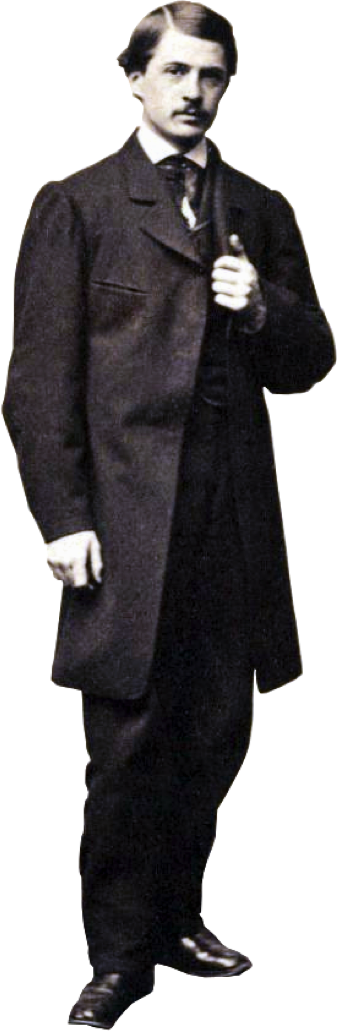
\includegraphics[width=1.7cm]{../figures/photo_pierce.png}
      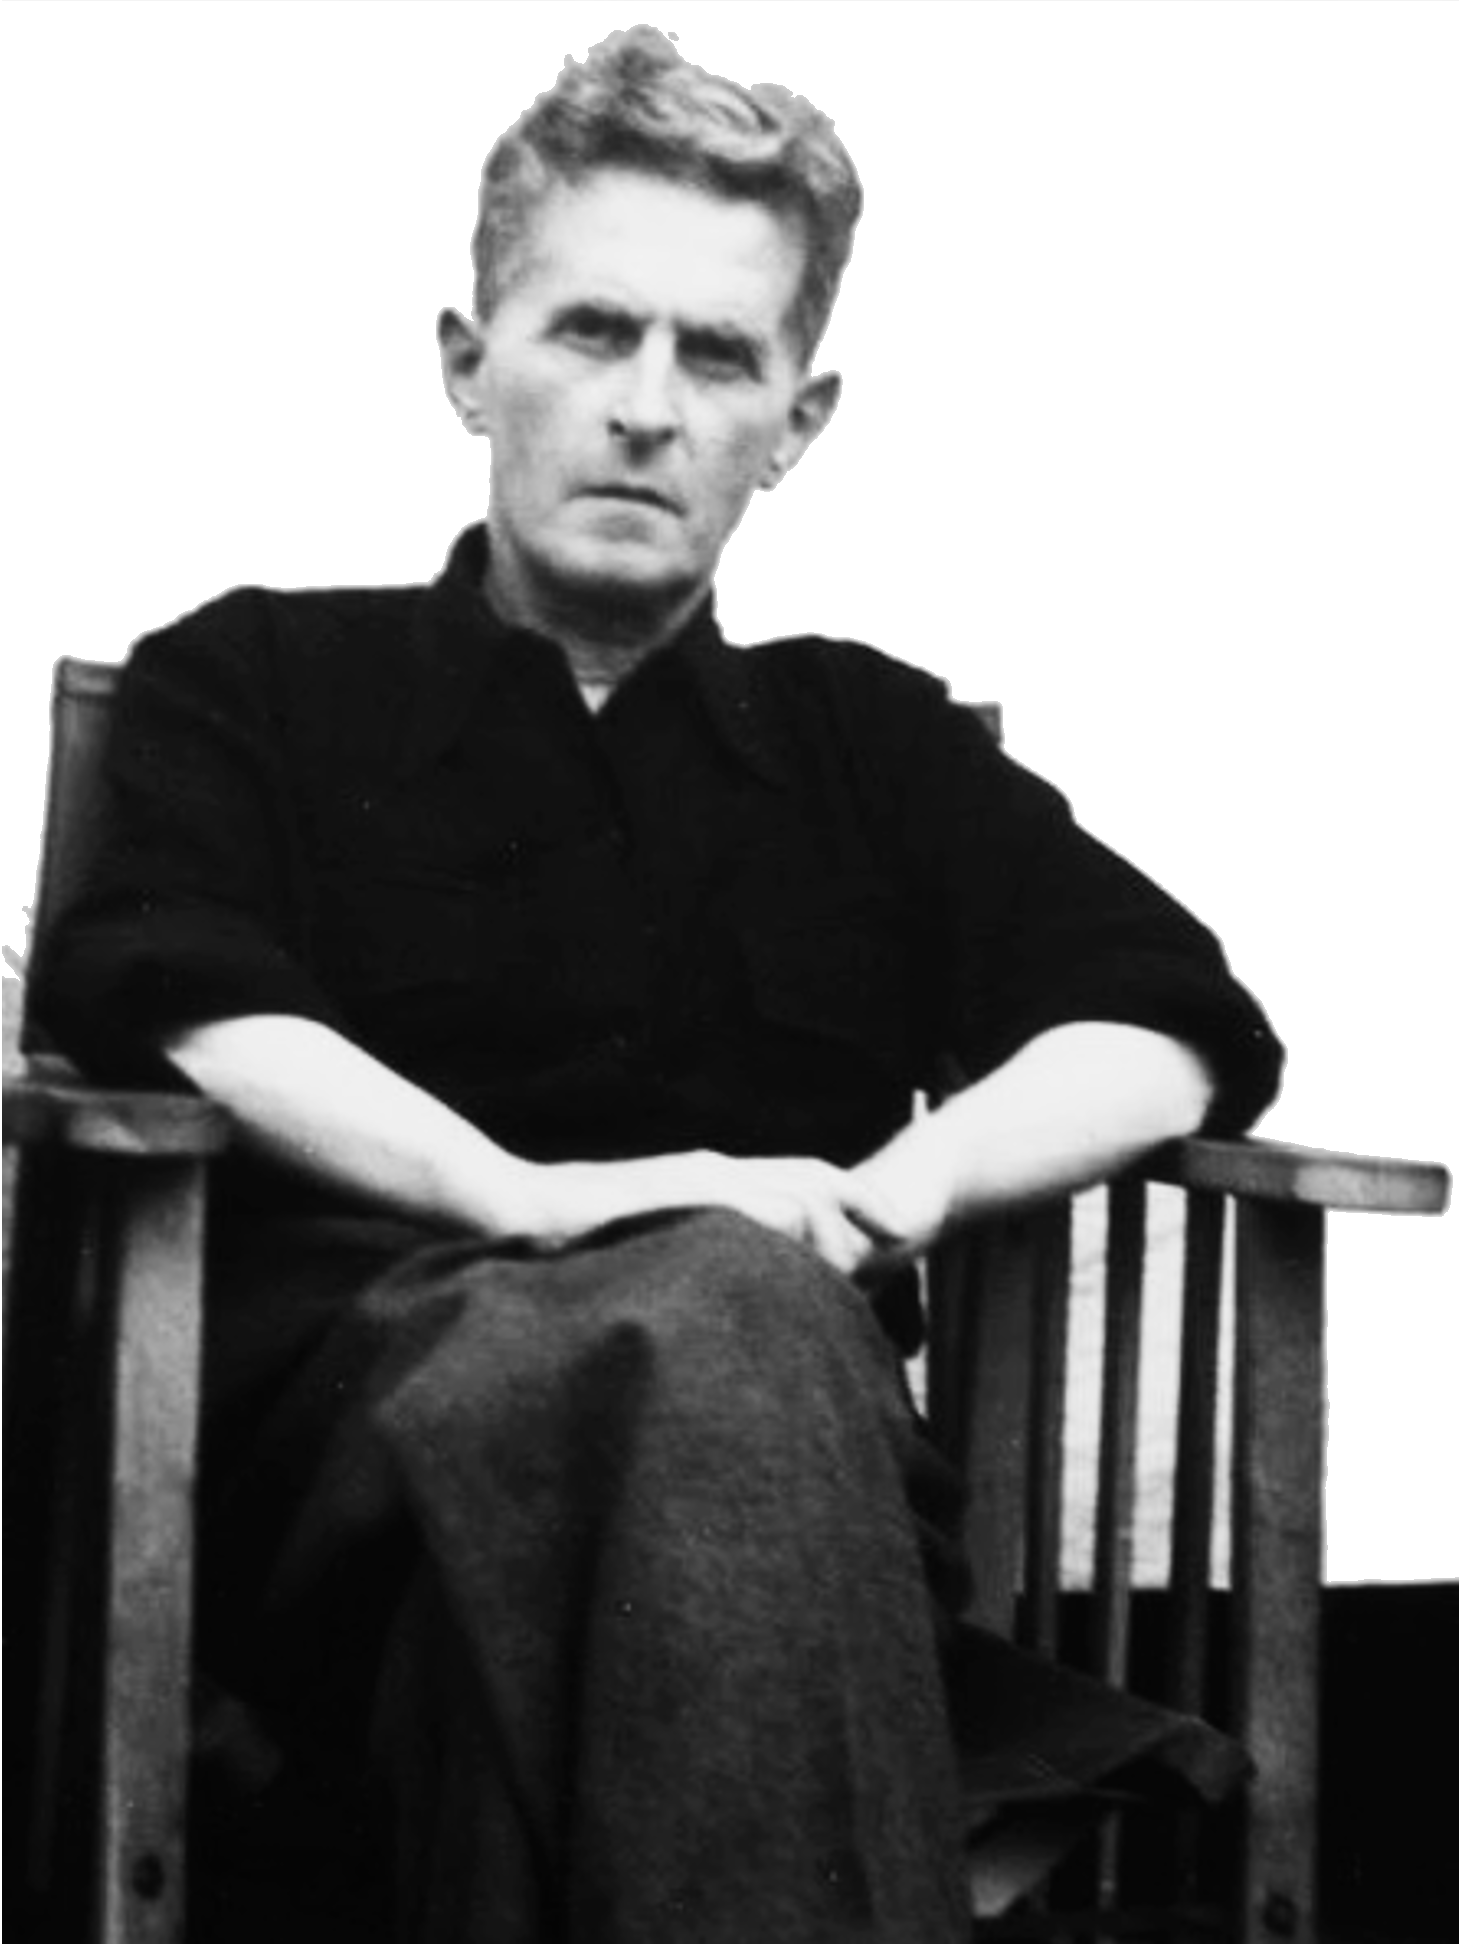
\includegraphics[width=2.6cm]{../figures/photo_wittgenstein.png}
    \end{column}
  \end{columns}
\end{frame}

%\begin{frame}[fragile]{Common sources of syntax errors}
%  \begin{itemize}
%    \item Reading impairments (e.g., dyslexia, dysgraphia)
%    \item Motor impairments (e.g., tremors, Parkinson's)
%    \item Speech impediments (e.g., stuttering, apraxia, Tourette's)
%    \item Visual impairments (e.g., poor eyesight, blindness)
%    \item Language barriers (e.g., foreign and non-native speakers)
%    \item Inexperience (e.g., novice programmers)
%    \item Distraction (e.g., multitasking, fatigue, stress)
%    \item Time pressure (e.g., deadlines, interview coding)
%    \item Inattention (e.g., typographic mistakes, boredom, apathy)
%    \item Lack of feedback (e.g., no syntax highlighting or IDE)
%  \end{itemize}
%\end{frame}

\begin{frame}{From Error-Correcting Codes to Correcting Coding Errors}
  \begin{itemize}
    \item Error-correcting codes are a well-studied topic in information theory used to detect and correct errors in data transmission.
    \item Introduces parity bits to detect and correct transmission errors assuming a certain noise model (e.g., Hamming distance).
    \item Like ECCs, we also assume a certain noise model (Levenshtein distance) and error tolerance (n-lexical tokens).
    \item Instead of injecting parity bits, we use the grammar and mutual information between tokens to detect and correct errors.
    \item Unlike ECCs, we do not assume a unique solution, but a set of admissible solutions ranked by statistical likliehood.
    \end{itemize}
  \setlength{\epigraphwidth}{0.97\textwidth}
  \epigraph{``\textit{Damn it, if the machine can detect an error, why can't it\\\phantom{``}locate the position of the error and correct it?'}''}{Richard Hamming, 1915-1998}
\end{frame}

\begin{frame}[fragile]{Syntax repair as a language game}
  \begin{itemize}
    \item Imagine a game between two players, \textit{Editor} and \textit{Author}.
    \item They both see the same grammar, $\mathcal{G}$ and invalid string $\err\sigma \notin \mathcal{L}(\mathcal{G})$.
    % Both players move simultaneously after a short period of deliberation. As soon as Player A repairs $\err\sigma$, Player B must move immediately.
    \item Author moves by modifying $\err\sigma$ to produce a valid string, $\sigma \in \mathcal{L}(\mathcal{G})$.
    \item Editor moves continuously, sampling a set $\tilde{\bm\sigma} \subseteq \mathcal{L}(\mathcal{G})$.
    \item As soon as Author repairs $\err\sigma$, the turn immediately ends.
    \item Neither player sees the other's move(s) before making their own.
    \item If Editor anticipates Author's move, i.e., $\sigma \in \tilde{\bm\sigma}$, they both win.
    \item If Author surprises Editor with a valid move, i.e., $\sigma \notin \tilde{\bm\sigma}$, Author wins.
    \item We may consider a refinement where Editor wins in proportion to the time taken to anticipate Author's move.
  \end{itemize}
\end{frame}

\begin{frame}[fragile]{Problem Statement: Validity and naturalness}
  Syntax repair can be treated as a language intersection problem between a context-free language (CFL) and a regular language.

  \begin{definition}[Reachable edits]
    Given a CFL, $\ell$, and an invalid string, $\err{\sigma}: \ell^\complement$, find every valid string reachable within $d$ edits of $\err{\sigma}$, i.e., letting $\Delta$ be the Levenshtein metric and $L(\err\sigma, d) = \{\sigma' \mid \Delta(\err{\sigma}, \sigma') \leq d\}$ be the edit ball, we seek $A = L(\err\sigma, d) \cap \ell$.
  \end{definition}

  \begin{definition}[Ranked repair]
  Given a finite language $A = L(\err\sigma, d) \cap \ell$ and a probabilistic language model $\text{P}_\theta: \Sigma^* \rightarrow [0, 1] \subset \mathbb{R}$, the ranked repair problem is to find the top-$k$ maximum likelihood repairs under the language model. That is,
  \begin{equation}
    R(A, P_\theta) = \argmax_{\bm{\sigma} \subseteq A, |\bm{\sigma}| \leq k} \sum_{\sigma \in \bm{\sigma}}\text{P}_\theta(\sigma)
  \end{equation}
    \end{definition}
%  To solve this problem, we will first pose a simpler problem that only considers localized edits, then turn our attention back to BCFLR.
%
%  \begin{definition}[Porous completion]
%    Let $\underline\Sigma \coloneqq \Sigma \cup \{\hole\}$, where \hole denotes a hole. We denote $\sqsubseteq: \Sigma^n \times \underline\Sigma^n$ as the relation $\{\langle\sigma', \sigma\rangle \mid \sigma_i \in \Sigma \implies \sigma_i' = \sigma_i\}$ and the set of all inhabitants $\{\sigma' \mid \sigma' \sqsubseteq \sigma\}$ as $\text{H}(\sigma)$. Given a \textit{porous string}, $\sigma: \underline\Sigma^*$ we seek all syntactically admissible inhabitants, i.e., $A(\sigma)\coloneqq\text{H}(\sigma)\cap\ell$.
%  \end{definition}
\end{frame}

\begin{frame}[fragile]{Problem Statement: Temporal constraints}
  Find every syntactically admissible edit $\{\sigma' \in \ell \mid \Delta(\err{\sigma}, \sigma') \leq d\}$, ranked by a probability metric $P_\theta$, and return them in a reasonable amount of time.

  \begin{definition}[Linear convergence]\label{def:linear-convergence}
  Given a finite CFL, $\ell$, we want a generating function, $\bm{\varphi}: \mathbb{N}_{<|\ell|} \rightarrow 2^\ell$, that converges linearly in expectation, i.e., $\mathbb{E}_{i \in [1, n]}|\bm{\varphi}(i)| \propto n$.
  \end{definition}

  \begin{center}
    \resizebox{0.42\textwidth}{!}{
      \def\secondcirclepath{(1.15,0) coordinate (e) circle (2cm)}
      \begin{tikzpicture}[
        dot/.style = {circle, inner sep=0pt, minimum size=1mm, fill,
        node contents={}}
      ]
        \def\firstcircle{(-2.1,0) coordinate (a) circle (2.4cm)}
        \def\firstcirclea{(-2.1,0) coordinate (b) circle (0.6cm)}
        \def\firstcircleb{(-2.1,0) coordinate (c) circle (1.2cm)}
        \def\firstcirclec{(-2.1,0) coordinate (d) circle (1.8cm)}
        \def\secondcircle{(1.2,0) coordinate (e) circle (1.5cm)}

        \begin{scope}
          \clip[decorate, decoration={snake, amplitude=0.6mm, segment length=5.01mm}] \secondcirclepath;
          \fill[black!15] \firstcircle;
        \end{scope}

        \draw \firstcircle node[dot,label=$\err{\sigma}$](z0);
        \draw [dashed] \firstcirclea;
        \draw [dashed] \firstcircleb;
        \draw [dashed] \firstcirclec;
        \draw[-stealth] (-2.1,0) -- (-1.5, 0) node[midway,below]{$d_1$};
        \draw[-stealth] (-1.5,0) -- (-0.9, 0) node[midway,below]{$d_2$};
        \draw[-stealth] (-0.9,0) -- (-0.3, 0) node[midway,below]{$d^*$};
        \draw[-stealth] (-0.3,0) -- (0.3, 0) node[midway,above]{$\tilde{\sigma}$};
        \draw[-stealth] (-0.3,0) -- (0.3, 0) node[midway,below]{$d^+$};

        \draw[decorate, decoration={snake, amplitude=0.6mm, segment length=5.01mm}] \secondcirclepath;
        \node [above] at (current bounding box.north -| a) {$\mathcal{L}\bigl(L(\err\sigma, d^*)\bigr)$};
        \node [above,yshift=2.1cm] at (e) {$\mathcal{L}(\mathcal{G}')$};
      \end{tikzpicture}
    }
    \scalebox{7}{\large$^+$\raisebox{0.2ex}{\huge\fontspec{Arial Unicode MS}^^^^231b}}
  \end{center}

  \textbf{Natural language:}
  \textit{Retrieve as many syntactically valid repairs as possible within a small neighborhood and time frame, ranked by naturalness.}
\end{frame}

%\begin{frame}[fragile]{Ranked repair under realtime constraints}
%  $A(\sigma)$ is often a very large-cardinality set, so we want a procedure which prioritizes likely repairs first, without exhaustive enumeration. Specifically,
%  \begin{definition}[Ranked repair]
%    Given a finite language $\ell_\cap = L(\err\sigma, d) \cap \ell$ and a probabilistic language model $P_\theta: \Sigma^* \rightarrow [0, 1] \subset \mathbb{R}$, the ranked repair problem is to find the top-$k$ repairs by likelihood under the language model. That is,
%    \begin{equation}
%      R(\ell_\cap, P_\theta) \coloneqq \argmax_{\{\bm{\sigma} \mid \bm{\sigma} \subseteq \ell_\cap, |\bm{\sigma}| \leq k\}} \sum_{\sigma \in \bm{\sigma}}\text{P}(\sigma\mid\err\sigma, \theta)
%    \end{equation}
%    % On average, across all $G, \sigma$ $\hat{R}$ should approximate $R$.
%    We want a procedure $\hat{R}$, minimizing $\mathbb{E}_{G, \sigma}\big[D_{\text{KL}}(\hat{R} \parallel R)\big]$ and total latency.
%  \end{definition}
%
%  Since $R$ is intractable in general, we want a procedure that approximates it for a representative sampling of natural context-free grammars and strings, i.e., real-world programming languages and source code snippets.
%\end{frame}

%\begin{frame}[fragile]{From CFL Reachability to Real World Program Repair}
%  To fix real code, we needed to overcome a variety of interesting challenges:\vspace{10pt}
%
%  \begin{itemize}
%    \item \textbf{Syntax mismatch}: The syntax of real-world programming languages does not exactly correspond to the theory of formal languages.
%    \item \textbf{Source code $\approx$ PL}: Most of the time, source code in the wild is incomplete or only loosely approximates a programming language.
%    \item \textbf{Responsiveness}: The usefulness of synthetic repairs is inversely proportional to the amount of time required to generate them.
%    \item \textbf{Edit generation}: How do we generate edits that are (1) syntactically admissible (2) statistically plausible and (3) semantically meaningful?
%    \item \textbf{Evaluation}: Big code and version control is too coarse-grained, contains irrelevant edits, not representative of small errors/fixes.
%  \end{itemize}
%\end{frame}


\begin{frame}[fragile]{High-level architecture overview}
  \vspace{0.4cm}
  \begin{figure}[h!]
    \vspace{-1cm}
      \begin{center}
      \resizebox{0.7\textwidth}{!}{
      \begin{tikzpicture}[node distance=5cm]
      \node (start) [io] {Broken code};
      \node (node1) [plain, right of=start] {\phantom{...}\textbf{Language intersection}\phantom{...}};
      \node (gram1) [io2, above of=node1, yshift=-3.2cm] {Grammar};
      %        \node (node2) [plain, right of=node1] {\textbf{Repair extraction}};
      %        \node (ptree) [io, above of=node2, yshift=-3cm] {$\mathbb{T}_2$};
      \node (node3) [plain, right of=node1, xshift=0.5cm] {\textbf{Repair decoding}};
      \node (ngram) [io2, above of=node3, yshift=-3.2cm] {Markov chain};
      \node (node4) [io, right of=node3] {Repairs};
      \draw [arrow] (start) -- (node1);
      \draw [arrow] (gram1) -- (node1);
      \draw [arrow] (node1) -- (node3);
      \draw [arrow] (node3) -- (node4);
      \draw [arrow] (ngram) -- (node3);
      %        \draw [arrow] (ptree) -- (node2);
      \end{tikzpicture}
      }
      \end{center}
  \end{figure}

  \vspace{0.4cm}

\begin{wrapfigure}{r}{0.4\textwidth}
%\begin{figure}[h!]
\vspace{-0.7cm}
\resizebox{0.4\textwidth}{!}{
\begin{tikzpicture}[node distance=2cm]
\node (start) [startstop, draw=none];
\node (pro1) [process, below of=start, yshift=-0.3cm] {$G_\cap \gets G\cap L(\err\sigma, d)$};
\node (pcfg) [io2, left of=pro1, xshift=-3cm] {CFG};
\node (lnfa) [io, right of=pro1, xshift=3cm] {L-NFA};

\node (code) [io, right of=start,xshift=3cm] {Code};
\node (synt) [io2, left of=start,xshift=-3cm] {Syntax};

\node (dec1) [decision, below of=pro1, yshift=-0.5cm] {$[G_{\cap} = \varnothing]$};

\node (t2) [process, left of=dec1, xshift=-3cm] {Construct $\mathbb{T}_2$ from $G_\cap'$};

\node (pro2b) [process, right of=dec1, xshift=3cm] {Increase radius, $d$};

\node [below=0.7cm of pro2b, xshift=-0.3cm] {\Large\textbf{Language intersection}};
\draw[thick,dotted, rounded corners] ($(pcfg.north west)+(-1.9,0.8)$) rectangle ($(pro2b.south east)+(0.3,-1.5)$);

\node (const) [process, below of=dec1, yshift=-1.8cm, xshift=-1.5cm] {Enumerate trees from $\mathbb{T}_2$};

%          \node (dec2) [decision, below of=const, yshift=-0.5cm] {$|\mathcal{L}(G_\cap)|$};
%
%          \node (samp1) [process, left of=dec2, xshift=-3cm] {Enumerate $\sigma' \in \mathcal{L}(G_\cap)$};
%          \node [above=0.07cm of samp1] {(\S~\ref{sec:ptree})};
%          \node (samp2) [process, right of=dec2, xshift=3cm] {Sample $\sigma' \sim P(G_\cap)$};
%          \node [above=0.07cm of samp2] {(\S~\ref{sec:ptree})};

%          \draw[thick,dotted, rounded corners] ($(const.north west)+(-5.3,0.7)$) rectangle ($(samp2.south east)+(0.3,-0.6)$);

\node (rrpc) [process, below of=const, yshift=-0.5cm] {Rerank by PCFG score};
\node [above=0.07cm of rrpc, xshift=1.7cm] {(Algorithm 1)};
\node (rank) [process, below of=rrpc, yshift=-0.5cm] {Convert to DFA and walk};
\node [above=0.1cm of rank, xshift=1.7cm] {(Algorithm 3)};
%          \node (vlmc) [io2, right of=rank, xshift=3cm] {Markov chain};
\node [below=0.3cm of rank, xshift=-3.8cm] {\Large\textbf{Repair decoding}};
\draw [thick,dotted, rounded corners] ($(rank.north west)+(-3.8,5.8)$) rectangle ($(rank.south east)+(6.8,-1.1)$);

\node (rrng) [process, right of=const, xshift=4.5cm] {Rerank by n-gram score};
\node [above=0.1cm of rrng, xshift=0.7cm] {(Algorithm 2)};
\node (results) [io, right of=rank, xshift=4.5cm] {Repairs};
%  \node (out1) [io, below of=pro2a] {Output};
\node (stop) [startstop, right of=rank, xshift=3cm];
\node (stop1) [startstop, right of=rrpc, xshift=3cm];
\node (stop2) [startstop, right of=const, xshift=3cm];

%  \draw [arrow] (dec0) -- node[anchor=east] {no} (pro1);

%          \draw [->,thick] (-5, 1.3) -- (synt);
%          \draw [->,thick] (5, 1.3) -- (code);

%          \draw [arrow] (start) -- (code);
%          \draw [arrow] (start) -- (synt);
\draw [arrow] (code) -- (lnfa);
\draw [arrow] (const) -- (rrng);
\draw [arrow] (rrng) -- (results);
\draw [arrow] (synt) -- (pcfg);
\draw [arrow] (lnfa) -- (pro1);
\draw [arrow] (pcfg) -- (pro1);

%          \draw [arrow] (grwa) -- (results);
%          \draw [line width=0.8pt] (stop.west) -- (stop1.west);
%          \draw [line width=0.8pt] (stop2.west) -- (stop1.west);

%  \draw [arrow] (in1) -- (pro1);
\draw [arrow] (pro1) -- (dec1);
\draw [arrow] (dec1) -- node[anchor=south] {yes} (pro2b);
\draw [arrow] (dec1) -- node[anchor=south] {no} (t2);
\draw [arrow] (const) -- (rrpc);
\draw [arrow] (pro2b) -- (lnfa);
%          \draw [arrow] (dec2) -- node[anchor=south] {small} (samp1);
%          \draw [arrow] (dec2) -- node[anchor=south] {large} (samp2);

\draw [arrow] (t2) |- ([shift={(-1.3cm,0)}]const.west)--(const.west);
%          \draw [arrow] (t2) |- ([shift={(-1.3cm,0)}]grwa.west)--(grwa.west);
\draw [arrow] (t2) |- ([shift={(-1.3cm,0)}]rank.west)--(rank.west);
%          \draw [arrow] (vlmc) -- (rank);
\draw [arrow] (rrpc) |- ([shift={(4.37cm,0)}]rrpc.east)--(results.north);
%          \draw [arrow] (samp2) |- ([shift={(0,1.3cm)}]rank.north)--(rank.north);
%  \draw [arrow] (pro2a) -- (out1);
\draw [arrow] (rank) -- (results);
%          \draw [line width=0.8pt] (grwa) -- (stop1);
%          \draw [line width=0.8pt] (const) -- (stop2);
%          \draw [arrow] (dec2) -- node[anchor=east] {1} (stop);

\end{tikzpicture}
}
\end{wrapfigure}

  Our syntax repair procedure can be described in three high-level steps. First, we generate a synthetic grammar $(G_\cap)$ representing the intersection between the syntax $(G)$ and Levenshtein ball around the source code $\big(\Delta(\err\sigma, d)\big)$. During repair extraction, we retrieve as many repairs as possible from the intersection grammar via sampling or enumeration. Finally, we rank all repairs discovered by likelihood.

\end{frame}


\begin{frame}[fragile]{High-level architecture overview}
This process can be depicted as series of staged transformations lowering the CFL intersection problem onto a finite automaton. Below, we consider a simplified version based on the language of balanced parentheses.

\vspace{0.3cm}
\begin{figure}[H]
\centering
\includegraphics[width=\textwidth]{flow_short.pdf}
\vspace{0.1cm}
\caption{Simplified dataflow of the language intersection pipeline. Given a grammar and broken code fragment, we (1) create a automaton generating the language of small edits, then (2) construct a grammar representing the intersection of the two languages. This grammar can be (3) converted into a finite automaton, (4) determinized, then (5) decoded to produce a list of repairs.}
\label{fig:exampleDFA}
\end{figure}
\end{frame}

\section{Formal Language Theory}\label{sec:fltheory}

%------------------------------------------------------------------------------------------------

\begin{frame}[fragile]{Background: Regular grammars}
  A regular grammar (RG) is a quadruple $\mathcal{G} = \langle V, \Sigma, P, S\rangle$ where $V$ are nonterminals, $\Sigma$ are terminals, $P: V\times (V \cup \Sigma)^{\leq 2}$ are the productions, and $S\in V$ is the start symbol, i.e., all productions are of the form $A \rightarrow a$, $A \rightarrow a B$ (right-regular), or $A \rightarrow B a$ (left-regular). E.g., the following RG and NFA correspond to the language defined by the \textit{regex} \tinline{(a(ab)*)*(ba)*}:

  % https://www3.nd.edu/~kogge/courses/cse30151-fa17/Public/other/tikz_tutorial.pdf
  % Glushkov's algorithm: https://www.irif.fr/~jep/PDF/MPRI/MPRI.pdf#subsection.3.5.2
  \begin{figure}
    \hspace{-1cm}
    \begin{minipage}[t]{0.25\linewidth}
      \vspace{-2.4cm}\scalebox{0.6}{
        \begin{aligned}[t]
          S &\rightarrow Q_0 \mid Q_2 \mid Q_3 \mid Q_5\\
          Q_0 &\rightarrow \varepsilon \\
          Q_1 &\rightarrow Q_0 b \mid Q_2 b\\
          Q_2 &\rightarrow Q_1 a \\
          Q_3 &\rightarrow Q_0 a \mid Q_3 a \mid Q_5 a \\
          Q_4 &\rightarrow Q_3 a \mid Q_5 a \\
          Q_5 &\rightarrow Q_4 b \\
        \end{aligned}}
    \end{minipage}
    \hspace{0.5cm}
    \begin{minipage}[t]{0.48\linewidth}
      \scalebox{0.5}{
        \begin{tikzpicture}
          [->, >=stealth,]
          \node[state, initial above, accepting] (Q0) {$Q_0$};
          \node[state, left of=Q0] (Q1) {$Q_1$};
          \node[state, accepting, left of=Q1] (Q2) {$Q_2$};
          \node[state, accepting, right of=Q0] (Q3) {$Q_3$};
          \node[state, above right of=Q3] (Q4) {$Q_4$};
          \node[state, accepting, below right of=Q3] (Q5) {$Q_5$};
          \draw
          %        (Q0) edge[loop above] (Q0)
          (Q0) edge node{\ttinline b} (Q1)
          (Q0) edge node{\ttinline a} (Q3)
          (Q1) edge[bend right] node{\ttinline a} (Q2)
          (Q2) edge[bend right] node{\ttinline b} (Q1)
          (Q3) edge[loop above] node{\ttinline a} (Q3)
          (Q3) edge node{\ttinline a} (Q4)
          (Q5) edge node{\ttinline a} (Q3)
          (Q4) edge[bend left] node{\ttinline b} (Q5)
          (Q5) edge[bend left] node{\ttinline a} (Q4)
        \end{tikzpicture}
      }
    \end{minipage}
  \end{figure}

  \begin{center}
    \scalebox{0.8}{
      \begin{tikzpicture}[font=\sffamily,breathe dist/.initial=4ex]
        \foreach \X [count=\Y,remember=\Y as \LastY] in
          {finite,regular}
          {\ifnum\Y=1
        \node[ellipse,draw,outer sep=0pt] (F-\Y) {\X};
        \else
        \path[decoration={text along path,
        text={|\sffamily|\X},text align=center,raise=0.9ex},decorate]
        let \p1=($(F-\LastY.north)-(F-\LastY.west)$)
        in (F-\LastY.west) arc(180:0:\x1 and \y1);
        \path let \p1=($([yshift=\pgfkeysvalueof{/tikz/breathe dist}]F-\LastY.north)
        -(F-\LastY.south)$),
        \p2=($(F-1.east)-(F-1.west)$),\p3=($(F-1.north)-(F-1.south)$)
        in ($([yshift=\pgfkeysvalueof{/tikz/breathe dist}]F-\LastY.north)!0.5!(F-\LastY.south)$)
        node[minimum height=\y1,minimum width={\y1*\x2/\y3},
        draw,ellipse,inner sep=0pt, fill=black!30!white] (F-\Y){};
        \fi
        }
        \foreach \X [count=\Y,remember=\Y as \LastY] in
          {finite,regular,context-free}
          {\ifnum\Y=1
        \node[ellipse,draw,outer sep=0pt] (F-\Y) {\X};
        \else
        \path[decoration={text along path,
        text={|\sffamily|\X},text align=center,raise=0.9ex},decorate]
        let \p1=($(F-\LastY.north)-(F-\LastY.west)$)
        in (F-\LastY.west) arc(180:0:\x1 and \y1);
        \path let \p1=($([yshift=\pgfkeysvalueof{/tikz/breathe dist}]F-\LastY.north)
        -(F-\LastY.south)$),
        \p2=($(F-1.east)-(F-1.west)$),\p3=($(F-1.north)-(F-1.south)$)
        in ($([yshift=\pgfkeysvalueof{/tikz/breathe dist}]F-\LastY.north)!0.5!(F-\LastY.south)$)
        node[minimum height=\y1,minimum width={\y1*\x2/\y3},
        draw,ellipse,inner sep=0pt] (F-\Y){};
        \fi}
      \end{tikzpicture}
    }
  \end{center}
\end{frame}

    \begin{frame}[fragile]{Levenshtein automaton customization}

Consider the string $\err\sigma=$ \texttt{\scriptsize ( ) )} and the alphabet $\Sigma = \{\texttt{\scriptsize)}, \texttt{\scriptsize(}\}$. Every string within one edit of $\err\sigma$ is recognizing by an NFA with the following structure:

\begin{figure}[h!]
\resizebox{0.45\textwidth}{!}{
\begin{tikzpicture}[
%->, % makes the edges directed
>=stealth',
node distance=2.5cm, % specifies the minimum distance between two nodes. Change if necessary.
%  every state/.style={thick, fill=gray!10}, % sets the properties for each ’state’ node
initial text=$ $, % sets the text that appears on the start arrow
]
\node[state, initial]                (00) {$q_{0,0}$};
\node[state, right of=00]            (10) {$q_{1,0}$};
\node[accepting, state, right of=10] (20) {$q_{2,0}$};
\node[accepting, state, right of=20] (30) {$q_{3,0}$};

\node[state, above of=00, shift={(-2cm,0cm)}] (01) {$q_{0,1}$};
\node[state, right of=01]                     (11) {$q_{1,1}$};
\node[state, right of=11]                     (21) {$q_{2,1}$};
\node[accepting, state, right of=21]          (31) {$q_{3,1}$};

\draw [->] (00) edge[below] node{$\texttt{(}$} (10);
\draw [->] (10) edge[below] node{$\texttt{)}$} (20);
\draw [->] (20) edge[below] node{$\texttt{)}$} (30);

\draw [->] (01) edge[below] node{$\texttt{(}$}                       (11);
\draw [->] (11) edge[below] node[shift={(-0.2cm,0cm)}]{$\texttt{)}$} (21);
\draw [->] (21) edge[below] node[shift={(-0.2cm,0cm)}]{$\texttt{)}$} (31);

\draw [->] (00) edge[bend left=10] node[shift={(-0.15cm,0cm)}]{\tiny{$\texttt{(}$}} (11);
\draw [->] (10) edge[bend left=10] node[shift={(-0.15cm,0cm)}]{\tiny{$\texttt{(}$}} (21);
\draw [->] (20) edge[bend left=10] node[shift={(-0.15cm,0cm)}]{\tiny{$\texttt{(}$}} (31);

\draw [->] (00) edge[bend left=10, left] node[shift={(-0.1cm,0cm)}]{\tiny{$\texttt{(}$}} (01);
\draw [->] (10) edge[bend left=10, left] node[shift={(-0.1cm,0cm)}]{\tiny{$\texttt{(}$}} (11);
\draw [->] (20) edge[bend left=10, left] node[shift={(-0.1cm,0cm)}]{\tiny{$\texttt{(}$}} (21);

\draw [->] (00) edge[bend right=10, right] node{\tiny{$\texttt{)}$}} (11);
\draw [->] (10) edge[bend right=10, right] node{\tiny{$\texttt{)}$}} (21);
\draw [->] (20) edge[bend right=10, right] node{\tiny{$\texttt{)}$}} (31);

\draw [->] (00) edge[bend right=10, right] node{\tiny{$\texttt{)}$}} (01);
\draw [->] (10) edge[bend right=10, right] node{\tiny{$\texttt{)}$}} (11);
\draw [->] (20) edge[bend right=10, right] node{\tiny{$\texttt{)}$}} (21);

\draw [->] (30) edge[bend left=10, left] node[shift={(-0.1cm,0cm)}]{\tiny{$\texttt{(}$}} (31);
\draw [->] (30) edge[bend right=10, right] node{\tiny{$\texttt{)}$}} (31);

\draw [->, blue] (00) edge[bend right=11,below] node[shift={(0.4cm,0.9cm)}]{$\texttt{)}$}    (21);
\draw [->, blue] (10) edge[bend right=11,below] node[shift={(0.4cm,0.9cm)}]{$\texttt{)}$}    (31);
\node[align=center, yshift=2em, xshift=-1cm] (title) at (current bounding box.north) {Original Levenshtein automaton};
\end{tikzpicture}
}
\resizebox{0.515\textwidth}{!}{
\begin{tikzpicture}[
%->, % makes the edges directed
>=stealth',
node distance=2.5cm, % specifies the minimum distance between two nodes. Change if necessary.
%  every state/.style={thick, fill=gray!10}, % sets the properties for each ’state’ node
initial text=$ $, % sets the text that appears on the start arrow
]
\draw[orange,->] (-4cm,1.2cm) -- (-3cm,1.2cm);

\node[state, initial]                (00) {$q_{0,0}$};
\node[state, right of=00]            (10) {$q_{1,0}$};
\node[accepting, state, right of=10] (20) {$q_{2,0}$};
\node[accepting, state, right of=20] (30) {$q_{3,0}$};

\node[state, above of=00, shift={(-2cm,0cm)}] (01) {$q_{0,1}$};
\node[state, right of=01]                     (11) {$q_{1,1}$};
\node[state, right of=11]                     (21) {$q_{2,1}$};
\node[accepting, state, right of=21]          (31) {$q_{3,1}$};

\draw [->] (00) edge[below] node{\tiny{$[= \texttt{(}]$}} (10);
\draw [->] (10) edge[below] node{\tiny{$[= \texttt{)}]$}} (20);
\draw [->] (20) edge[below] node{\tiny{$[= \texttt{)}]$}} (30);

\draw [->] (01) edge[below] node{\tiny{$[= \texttt{(}]$}}                       (11);
\draw [->] (11) edge[below] node[shift={(-0.2cm,0cm)}]{\tiny{$[= \texttt{)}]$}} (21);
\draw [->] (21) edge[below] node[shift={(-0.2cm,0cm)}]{\tiny{$[= \texttt{)}]$}} (31);

\draw [->] (00) edge[left] node{\tiny{$[\neq \texttt{(}]$}} (11);
\draw [->] (10) edge[left] node{\tiny{$[\neq \texttt{)}]$}} (21);
\draw [->] (20) edge[left] node{\tiny{$[\neq \texttt{)}]$}} (31);

\draw [->] (00) edge[bend left=10, left] node{\tiny{$[\neq \texttt{(}]$}} (01);
\draw [->] (10) edge[bend left=10, left] node{\tiny{$[\neq \texttt{)}]$}} (11);
\draw [->] (20) edge[bend left=10, left] node{\tiny{$[\neq \texttt{)}]$}} (21);
\draw [->] (30) edge[bend left=10, left] node{\tiny{$[=.]$}} (31);


\draw [->, blue] (00) edge[bend right=11,below] node[shift={(0.2cm,0.8cm)}]{\tiny{$[= \texttt{)}]$}}    (21);
\draw [->, blue] (10) edge[bend right=11,below] node[shift={(0.2cm,0.8cm)}]{\tiny{$[= \texttt{)}]$}}    (31);
\node[align=center, yshift=2em, xshift=-0.4cm] (title) at (current bounding box.north) {Nominal Levenshtein automaton (ours)};
\end{tikzpicture}
}
\caption{Automaton recognizing every single patch of the broken string \texttt{( ) )} within Levenshtein distance 1. We nominalize the original Levenshtein automaton, ensuring upward arcs denote a mutation, and replace terminals with a symbolic predicate, which deduplicates parallel arcs in large alphabets.}\label{fig:lev_automaton}\vspace{-5pt}
\end{figure}
\\
\tiny{\url{https://fulmicoton.com/posts/levenshtein/#observations-lets-count-states}}
\end{frame}

\begin{frame}[fragile]{Levenshtein reachability}
  \begin{figure}[H]
    \resizebox{\textwidth}{!}{
      \begin{tikzpicture}[
%->, % makes the edges directed
        >=stealth',
        node distance=2.5cm, % specifies the minimum distance between two nodes. Change if necessary.
%  every state/.style={thick, fill=gray!10}, % sets the properties for each ’state’ node
        initial text=$ $, % sets the text that appears on the start arrow
      ]
        \node[state, initial]                (00) {$q_{0,0}$};
        \node[state, right of=00]            (10) {$q_{1,0}$};
        \node[accepting, state, right of=10] (20) {$q_{2,0}$};
        \node[accepting, state, right of=20] (30) {$q_{3,0}$};
        \node[accepting, state, right of=30] (40) {$q_{4,0}$};
        \node[accepting, state, right of=40] (50) {$q_{5,0}$};

        \node[state, above of=00, shift={(-2cm,0cm)}] (01) {$q_{0,1}$};
        \node[state, right of=01]                          (11) {$q_{1,1}$};
        \node[state, right of=11]                          (21) {$q_{2,1}$};
        \node[accepting, state, right of=21]               (31) {$q_{3,1}$};
        \node[accepting, state, right of=31]               (41) {$q_{4,1}$};
        \node[accepting, state, right of=41]               (51) {$q_{5,1}$};

        \node[state, above of=01, shift={(-2cm,0cm)}] (0j) {$q_{0,2}$};
        \node[state, right of=0j]                          (1j) {$q_{1,2}$};
        \node[state, right of=1j]                          (2j) {$q_{2,2}$};
        \node[state, right of=2j]                          (3j) {$q_{3,2}$};
        \node[accepting, state, right of=3j]               (4j) {$q_{4,2}$};
        \node[accepting, state, right of=4j]               (5j) {$q_{5,2}$};

        \node[state, above of=0j, shift={(-2cm,0cm)}] (0k) {$q_{0,3}$};
        \node[state, right of=0k]                         (1k) {$q_{1,3}$};
        \node[state, right of=1k]                         (2k) {$q_{2,3}$};
        \node[state, right of=2k]                         (3k) {$q_{3,3}$};
        \node[state, right of=3k]                         (4k) {$q_{4,3}$};
        \node[accepting, state, right of=4k]              (5k) {$q_{5,3}$};

        \draw [->] (00) edge[below] node{$\sigma_1$} (10);
        \draw [->] (10) edge[below] node{$\sigma_2$} (20);
        \draw [->] (20) edge[below] node{$\sigma_3$} (30);
        \draw [->] (30) edge[below] node{$\sigma_4$} (40);
        \draw [->] (40) edge[below] node{$\sigma_5$} (50);

        \draw [->] (01) edge[below] node{$\sigma_1$} (11);
        \draw [->] (11) edge[below] node[shift={(-0.2cm,0cm)}]{$\sigma_2$} (21);
        \draw [->] (21) edge[below] node[shift={(-0.2cm,0cm)}]{$\sigma_3$} (31);
        \draw [->] (31) edge[below] node[shift={(-0.2cm,0cm)}]{$\sigma_4$} (41);
        \draw [->] (41) edge[below] node{$\sigma_5$} (51);

        \draw [->] (0j) edge[below] node{$\sigma_1$} (1j);
        \draw [->] (1j) edge[below] node{$\sigma_2$} (2j);
        \draw [->] (2j) edge[below] node{$\sigma_3$} (3j);
        \draw [->] (3j) edge[below] node{$\sigma_4$} (4j);
        \draw [->] (4j) edge[below] node{$\sigma_5$} (5j);

        \draw [->] (0k) edge[below] node{$\sigma_1$} (1k);
        \draw [->] (1k) edge[below] node{$\sigma_2$} (2k);
        \draw [->] (2k) edge[below] node{$\sigma_3$} (3k);
        \draw [->] (3k) edge[below] node{$\sigma_4$} (4k);
        \draw [->] (4k) edge[below] node{$\sigma_5$} (5k);

        \draw [->] (00) edge[left] node{$\phantom{\cdot}$} (11);
        \draw [->] (10) edge[left] node{$\phantom{\cdot}$} (21);
        \draw [->] (20) edge[left] node{$\phantom{\cdot}$} (31);
        \draw [->] (30) edge[left] node{$\phantom{\cdot}$} (41);
        \draw [->] (40) edge[left] node{$\phantom{\cdot}$} (51);

% Super-knight arcs
        \draw [->, red] (00) edge[bend right=8] node[east, shift={(-0.2cm,-0.7cm)}]{$\color{red}\sigma_3$}         (3j);
        \draw [->, red] (10) edge[bend right=8] node[east, shift={(-0.2cm,-0.7cm)}]{$\color{red}\sigma_4$}         (4j);
        \draw [->, red] (20) edge[bend right=8] node[east, shift={(-0.2cm,-0.7cm)}]{$\color{red}\sigma_5$}         (5j);

        \draw [->, red] (01) edge[bend left=8] node[east, shift={(-0.2cm,-0.7cm)}]{$\color{red}\sigma_3$}         (3k);
        \draw [->, red] (11) edge[bend left=8] node[east, shift={(-0.2cm,-0.7cm)}]{$\color{red}\sigma_4$}         (4k);
        \draw [->, red] (21) edge[bend left=8] node[east, shift={(-0.2cm,-0.7cm)}]{$\color{red}\sigma_5$}         (5k);

        \draw [->, violet] (00) edge node[east, shift={(-0.1cm,-0.8cm)}]{$\color{violet}\sigma_4$}  (4k);
        \draw [->, violet] (10) edge node[east, shift={(-0.1cm,-0.8cm)}]{$\color{violet}\sigma_5$}  (5k);

        \draw [->] (01) edge[left] node{$\phantom{\cdot}$} (1j);
        \draw [->] (11) edge[left] node{$\phantom{\cdot}$} (2j);
        \draw [->] (21) edge[left] node{$\phantom{\cdot}$} (3j);
        \draw [->] (31) edge[left] node{$\phantom{\cdot}$} (4j);
        \draw [->] (41) edge[left] node{$\phantom{\cdot}$} (5j);

        \draw [->] (0j) edge[left] node{$\phantom{\cdot}$} (1k);
        \draw [->] (1j) edge[left] node{$\phantom{\cdot}$} (2k);
        \draw [->] (2j) edge[left] node{$\phantom{\cdot}$} (3k);
        \draw [->] (3j) edge[left] node{$\phantom{\cdot}$} (4k);
        \draw [->] (4j) edge[left] node{$\phantom{\cdot}$} (5k);

        \draw [->] (00) edge[bend left=10, left] node{$\phantom{\cdot}$} (01);
        \draw [->] (10) edge[bend left=10, left] node{$\phantom{\cdot}$} (11);
        \draw [->] (20) edge[bend left=10, left] node{$\phantom{\cdot}$} (21);
        \draw [->] (30) edge[bend left=10, left] node{$\phantom{\cdot}$} (31);
        \draw [->] (40) edge[bend left=10, left] node{$\phantom{\cdot}$} (41);
        \draw [->] (50) edge[bend left=10, left] node{$\phantom{\cdot}$} (51);

        \draw [->] (01) edge[bend left=10, left] node{$\phantom{\cdot}$} (0j);
        \draw [->] (11) edge[bend left=10, left] node{$\phantom{\cdot}$} (1j);
        \draw [->] (21) edge[bend left=10, left] node{$\phantom{\cdot}$} (2j);
        \draw [->] (31) edge[bend left=10, left] node{$\phantom{\cdot}$} (3j);
        \draw [->] (41) edge[bend left=10, left] node{$\phantom{\cdot}$} (4j);
        \draw [->] (51) edge[bend left=10, left] node{$\phantom{\cdot}$} (5j);

        \draw [->] (0j) edge[bend left=10, left] node{$\phantom{\cdot}$} (0k);
        \draw [->] (1j) edge[bend left=10, left] node{$\phantom{\cdot}$} (1k);
        \draw [->] (2j) edge[bend left=10, left] node{$\phantom{\cdot}$} (2k);
        \draw [->] (3j) edge[bend left=10, left] node{$\phantom{\cdot}$} (3k);
        \draw [->] (4j) edge[bend left=10, left] node{$\phantom{\cdot}$} (4k);
        \draw [->] (5j) edge[bend left=10, left] node{$\phantom{\cdot}$} (5k);

        \draw [->, blue] (00) edge[bend right=11,below] node[shift={(0.5cm,0.3cm)}]{$\color{blue}\sigma_2$}    (21);
        \draw [->, blue] (10) edge[bend right=11,below] node[shift={(0.5cm,0.3cm)}]{$\color{blue}\sigma_3$}    (31);
        \draw [->, blue] (20) edge[bend right=11,below] node[shift={(0.5cm,0.3cm)}]{$\color{blue}\sigma_4$}    (41);
        \draw [->, blue] (30) edge[bend right=11,below] node[shift={(0.5cm,0.3cm)}]{$\color{blue}\sigma_5$}    (51);

        \draw [->, blue] (01) edge[bend right=3,below] node[shift={(0.3cm,0.2cm)}]{$\color{blue}\sigma_2$}    (2j);
        \draw [->, blue] (11) edge[bend right=3,below] node[shift={(0.3cm,0.2cm)}]{$\color{blue}\sigma_3$}    (3j);
        \draw [->, blue] (21) edge[bend right=3,below] node[shift={(0.3cm,0.2cm)}]{$\color{blue}\sigma_4$}    (4j);
        \draw [->, blue] (31) edge[bend right=3,below] node[shift={(0.3cm,0.2cm)}]{$\color{blue}\sigma_4$}    (5j);

        \draw [->, blue] (0j) edge[bend left=8,below] node[shift={(-0.45cm,-0.55cm)}]{$\color{blue}\sigma_2$}    (2k);
        \draw [->, blue] (1j) edge[bend left=8,below] node[shift={(-0.45cm,-0.55cm)}]{$\color{blue}\sigma_3$}    (3k);
        \draw [->, blue] (2j) edge[bend left=8,below] node[shift={(-0.45cm,-0.55cm)}]{$\color{blue}\sigma_4$}    (4k);
        \draw [->, blue] (3j) edge[bend left=8,below] node[shift={(-0.45cm,-0.55cm)}]{$\color{blue}\sigma_5$}    (5k);

%https://tex.stackexchange.com/a/20986/139648
        \draw [decorate,decoration={brace,amplitude=10pt,raise=10pt,mirror}] (00.south west) -- (50.south east) node[midway,yshift=-3em]{\textbf{String length}};
        \draw [decorate,decoration={brace,amplitude=10pt,raise=20pt}] (00.south west) -- (0k.north west) node[midway,xshift=-1cm,yshift=-1cm,rotate=-54]{\textbf{Edit distance}};
      \end{tikzpicture}
    }
    \caption{Bounded Levenshtein reachability from $\sigma: \Sigma^n$ is expressible as an NFA populated by accept states within radius $k$ of $S=q_{n,0}$, which accepts all strings $\sigma'$ within Levenshtein radius $k$ of $\sigma$.}
  \end{figure}
\end{frame}

\begin{frame}[fragile]{Geometrically interpreting the edit calculus}

Each arc plays a specific role. $\duparrow$ handles insertions, $\ddiagarrow$ handles substitutions and $\knightarrow$ handles deletions of $\geq 1$ tokens. Consider some illustrative cases:

\vspace{0.5cm}

\newcommand{\substitutionExample}{
\tikz{
\foreach \x in {0,8,16,24,32,40}{
\fill (\x pt,0pt) circle [radius = 1pt];
\fill (\x pt,8pt) circle [radius = 1pt];
}
\phantom{\fill (0pt,-8pt) circle [radius = 1pt];}
\draw [-to] (0pt,0pt) -- (8pt,0pt);
\draw [-to] (8pt,0pt) -- (16pt,0pt);
\draw [-to] (16pt,0pt) -- (24pt,8pt);
\draw [-to] (24pt,8pt) -- (32pt,8pt);
\draw [-to] (32pt,8pt) -- (40pt,8pt);
}
}

\newcommand{\insertionExample}{
\tikz{
\foreach \x in {0,8,16,24,32,40}{
\fill (\x pt,0pt) circle [radius = 1pt];
\fill (\x pt,8pt) circle [radius = 1pt];
}
\phantom{\fill (0pt,-8pt) circle [radius = 1pt];}
\fill[white] (16pt,0pt) circle [radius = 1.2pt];
\fill[white] (24pt,8pt) circle [radius = 1.2pt];
\draw [-to] (0pt,0pt) -- (8pt,0pt);
\draw [-to] (8pt,0pt) -- (24pt,0pt);
\draw [-to] (24pt,0pt) -- (16pt,8pt);
\draw [-to] (16pt,8pt) -- (32pt,8pt);
\draw [-to] (32pt,8pt) -- (40pt,8pt);
}
}

\newcommand{\deletionExample}{
\tikz{
\foreach \x in {0,8,16,24,32,40}{
\fill (\x pt,0pt) circle [radius = 1pt];
\fill (\x pt,8pt) circle [radius = 1pt];
}
\phantom{\fill (0pt,-8pt) circle [radius = 1pt];}
\draw [-to] (0pt,0pt) -- (8pt,0pt);
\draw [-to] (8pt,0pt) -- (16pt,0pt);
\draw [-to] (16pt,0pt) -- (24pt,0pt);
\draw [-to] (24pt,0pt) -- (40pt,8pt);
}
}

\newcommand{\doubleDeletionExample}{
\tikz{
\foreach \x in {0,8,16,24,32,40}{
\fill (\x pt,0pt) circle [radius = 1pt];
\fill (\x pt,8pt) circle [radius = 1pt];
\fill (\x pt,16pt) circle [radius = 1pt];
}
\draw [-to] (0pt,0pt) -- (24pt,16pt);
\draw [-to] (24pt,16pt) -- (32pt,16pt);
\draw [-to] (32pt,16pt) -- (40pt,16pt);
}
}

\newcommand{\subDelExample}{
\tikz{
\foreach \x in {0,8,16,24,32,40}{
\fill (\x pt,0pt) circle [radius = 1pt];
\fill (\x pt,8pt) circle [radius = 1pt];
\fill (\x pt,16pt) circle [radius = 1pt];
}
\draw [-to] (0pt,0pt) -- (8pt,0pt);
\draw [-to] (8pt,0pt) -- (16pt,8pt);
\draw [-to] (16pt,8pt) -- (32pt,16pt);
\draw [-to] (32pt,16pt) -- (40pt,16pt);
}
}

\newcommand{\subSubExample}{
\tikz{
\foreach \x in {0,8,16,24,32,40}{
\fill (\x pt,0pt) circle [radius = 1pt];
\fill (\x pt,8pt) circle [radius = 1pt];
\fill (\x pt,16pt) circle [radius = 1pt];
}
\draw [-to] (0pt,0pt) -- (8pt,0pt);
\draw [-to] (8pt,0pt) -- (16pt,8pt);
\draw [-to] (16pt,8pt) -- (24pt,16pt);
\draw [-to] (24pt,16pt) -- (32pt,16pt);
\draw [-to] (32pt,16pt) -- (40pt,16pt);
}
}

\newcommand{\insertDeleteExample}{
\tikz{
\foreach \x in {0,8,16,24,32,40,48}{
\fill (\x pt,0pt) circle [radius = 1pt];
\fill (\x pt,8pt) circle [radius = 1pt];
\fill (\x pt,16pt) circle [radius = 1pt];
}
\fill[white] (16pt,16pt) circle [radius = 1.2pt];
\fill[white] (8pt,0pt) circle [radius = 1.2pt];
\fill[white] (16pt,8pt) circle [radius = 1.2pt];
\draw [-to] (0pt,0pt) -- (16pt,0pt);
\draw [-to] (16pt,0pt) -- (8pt,8pt);
\draw [-to] (8pt,8pt) -- (24pt,8pt);
\draw [-to] (24pt,8pt) -- (40pt,16pt);
\draw [-to] (40pt,16pt) -- (48pt,16pt);
}
}

\footnotesize{
\begin{table}[h!]
\begin{tabular}{ccccc}

\texttt{f\hspace{3pt}.\hspace{3pt}\hlorange{[}\hspace{3pt}x\hspace{3pt})} &
\texttt{f\hspace{3pt}.\hspace{3pt}\phantom{(}\hspace{3pt}x\hspace{3pt})} &
\texttt{f\hspace{3pt}.\hspace{3pt}(\hspace{3pt}\hlred{x}\hspace{3pt})} &
\texttt{\hlred{.}\hspace{3pt}\hlred{+}\hspace{3pt}(\hspace{3pt}x\hspace{3pt})} &
\texttt{f\hspace{3pt}\hlorange{.}\hspace{3pt}\hlred{(}\hspace{3pt}x\hspace{3pt};} \\

\texttt{f\hspace{3pt}.\hspace{3pt}\hlorange{(}\hspace{3pt}x\hspace{3pt})} &
\texttt{f\hspace{3pt}.\hspace{3pt}\hlgreen{(}\hspace{3pt}x\hspace{3pt})} &
\texttt{f\hspace{3pt}.\hspace{3pt}(\hspace{3pt}\phantom{x}\hspace{3pt})} &
\texttt{\phantom{f}\hspace{3pt}\phantom{.}\hspace{3pt}(\hspace{3pt}x\hspace{3pt})} &
\texttt{f\hspace{3pt}\hlorange{*}\hspace{3pt}\phantom{(}\hspace{3pt}x\hspace{3pt};} \\

\substitutionExample & \insertionExample & \deletionExample & \doubleDeletionExample & \subDelExample
\end{tabular}
\end{table}
}

\normalsize{Note that the same $\langle\err\sigma, \sigma'\rangle$ pair can have multiple Levenshtein alignments:}
\vspace{0.5cm}

\footnotesize{
\begin{table}[h!]
\begin{tabular}{cc}

\texttt{[\hspace{3pt}\hlorange{,}\hspace{3pt}\hlorange{x}\hspace{3pt}y\hspace{3pt}]} &
\texttt{[\hspace{3pt}\phantom{,}\hspace{3pt},\hspace{3pt}\hlred{x}\hspace{3pt}y\hspace{3pt}]} \\

\texttt{[\hspace{3pt}\hlorange{x}\hspace{3pt}\hlorange{,}\hspace{3pt}y\hspace{3pt}]} &
\texttt{[\hspace{3pt}\hlgreen{x}\hspace{3pt},\hspace{3pt}\phantom{x}\hspace{3pt}y\hspace{3pt}]} \\

\subSubExample & \insertDeleteExample
\end{tabular}
\end{table}
}

\normalsize{Non-uniqueness of geodesics has implications for CFG $\cap$ L-NFA ambiguity.}
\end{frame}

\begin{frame}[fragile]{The nominal Levenshtein automaton}
  The original Levenshtein automaton (Schulz \& Stoyan, 2002):

  \begin{prooftree}
    \AxiomC{$s\in\Sigma \phantom{\land} i \in [0, n] \phantom{\land} j \in [1, k]$}
    \RightLabel{$\duparrow$}
    \UnaryInfC{$(q_{i, j-1} \overset{s}{\rightarrow} q_{i,j}) \in \delta$}
    \DisplayProof
    \hskip 1.5em
    \AxiomC{$s\in\Sigma \phantom{\land} i \in [1, n] \phantom{\land} j \in [1, k]$}
    \RightLabel{$\ddiagarrow$}
    \UnaryInfC{$(q_{i-1, j-1} \overset{s}{\rightarrow} q_{i,j}) \in \delta$}
  \end{prooftree}
  \begin{prooftree}
    \AxiomC{$s=\sigma_i \phantom{\land} i \in [1, n] \phantom{\land} j \in [0, k]$}
    \RightLabel{$\drightarrow$}
    \UnaryInfC{$(q_{i-1, j} \overset{s}{\rightarrow} q_{i,j}) \in \delta$}
    \DisplayProof
    \hskip 1.5em
    \AxiomC{$s=\sigma_i \phantom{\land} i \in [2, n] \phantom{\land} j \in [1, k]$}
    \RightLabel{$\knightarrow$}
    \UnaryInfC{$(q_{i-2, j-1} \overset{s}{\rightarrow} q_{i,j}) \in \delta$}
  \end{prooftree}
  \begin{prooftree}
    \AxiomC{$\vphantom{|}$}
    \RightLabel{$\textsc{Init}$}
    \UnaryInfC{$q_{0,0} \in I$}
    \DisplayProof
    \hskip 1.5em
    \AxiomC{$q_{i, j}$}
    \AxiomC{$|n-i+j| \leq k$}
    \RightLabel{$\textsc{Done}$}
    \BinaryInfC{$q_{i, j}\in F$}
  \end{prooftree}

  We modify the original automaton with a nominal predicate:

  \begin{prooftree}
    \AxiomC{$i \in [0, n] \phantom{\land} j \in [1, k]$}
    \RightLabel{$\duparrow$}
    \UnaryInfC{$(q_{i, j-1} \overset{{\color{orange}[\neq \sigma_{i+1}]}}{\rightarrow} q_{i,j}) \in \delta$}
    \DisplayProof
    \hskip 1.5em
    \AxiomC{$i \in [1, n] \phantom{\land} j \in [1, k]$}
    \RightLabel{$\ddiagarrow$}
    \UnaryInfC{$(q_{i-1, j-1} \overset{{\color{orange}[\neq \sigma_i]}}{\rightarrow} q_{i,j}) \in \delta$}
  \end{prooftree}
  \begin{prooftree}
    \AxiomC{$i \in [1, n] \phantom{\land} j \in [0, k]$}
    \RightLabel{$\drightarrow$}
    \UnaryInfC{$(q_{i-1, j} \overset{{\color{orange}[=\sigma_i]}}{\rightarrow} q_{i,j}) \in \delta$}
    \DisplayProof
    \hskip 1.5em
    \AxiomC{$d \in [1, d_{\max}] \phantom{\land} i \in [d + 1, n] \phantom{\land} j \in [d, k]$}
    \RightLabel{$\knightarrow$}
    \UnaryInfC{$(q_{i-d-1, j-d} \overset{{\color{orange}[=\sigma_i]}}{\rightarrow} q_{i,j}) \in \delta$}
  \end{prooftree}
\end{frame}

\begin{frame}{Background: Context-free grammars}
  In a context-free grammar $\mathcal{G} = \langle V, \Sigma, P, S\rangle$ all productions are of the form $P: V\times (V \cup \Sigma)^+$, i.e., RHS may contain any number of nonterminals, $V$. Recognition decidable in $\mathcal{O}(n^\omega)$, n.b. CFLs are \textbf{not} closed under $\cap$!\newline\\
  %
  For example, consider the grammar $\underline{S \rightarrow S S \mid ( S ) \mid ()}$. This represents the language of balanced parentheses, e.g. $(), ()(), (()), ()(()), (()()), (())()\ldots$\newline\\
  %
  Every CFG has a normal form $P^*: V \times (V^2 \mid \Sigma)$, i.e., every production can be refactored into either $v_0 \rightarrow v_1 v_2$ or $v_0 \rightarrow \sigma$, where $v_{0\ldots2}: V$ and $\sigma: \Sigma$, e.g., $\{S \rightarrow S S \mid ( S ) \mid ()\}\Leftrightarrow^*\{S\rightarrow XR \mid SS \mid LR, L \rightarrow (, R \rightarrow ), X\rightarrow LS\}$

  \begin{center}
    \scalebox{0.8}{
      \begin{tikzpicture}[font=\sffamily,breathe dist/.initial=4ex]
        \foreach \X [count=\Y,remember=\Y as \LastY] in
          {finite,regular,context-free}
          {\ifnum\Y=1
        \node[ellipse,draw,outer sep=0pt] (F-\Y) {\X};
        \else
        \path[decoration={text along path,
        text={|\sffamily|\X},text align=center,raise=0.9ex},decorate]
        let \p1=($(F-\LastY.north)-(F-\LastY.west)$)
        in (F-\LastY.west) arc(180:0:\x1 and \y1);
        \path let \p1=($([yshift=\pgfkeysvalueof{/tikz/breathe dist}]F-\LastY.north)
        -(F-\LastY.south)$),
        \p2=($(F-1.east)-(F-1.west)$),\p3=($(F-1.north)-(F-1.south)$)
        in ($([yshift=\pgfkeysvalueof{/tikz/breathe dist}]F-\LastY.north)!0.5!(F-\LastY.south)$)
        node[minimum height=\y1,minimum width={\y1*\x2/\y3},
        draw,ellipse,inner sep=0pt, fill=black!30!white] (F-\Y){};
        \fi
        }
        \foreach \X [count=\Y,remember=\Y as \LastY] in
          {finite,regular,context-free,conjunctive}
          {\ifnum\Y=1
        \node[ellipse,draw,outer sep=0pt] (F-\Y) {\X};
        \else
        \path[decoration={text along path,
        text={|\sffamily|\X},text align=center,raise=0.9ex},decorate]
        let \p1=($(F-\LastY.north)-(F-\LastY.west)$)
        in (F-\LastY.west) arc(180:0:\x1 and \y1);
        \path let \p1=($([yshift=\pgfkeysvalueof{/tikz/breathe dist}]F-\LastY.north)
        -(F-\LastY.south)$),
        \p2=($(F-1.east)-(F-1.west)$),\p3=($(F-1.north)-(F-1.south)$)
        in ($([yshift=\pgfkeysvalueof{/tikz/breathe dist}]F-\LastY.north)!0.5!(F-\LastY.south)$)
        node[minimum height=\y1,minimum width={\y1*\x2/\y3},
        draw,ellipse,inner sep=0pt] (F-\Y){};
        \fi}
      \end{tikzpicture}
    }
  \end{center}
\end{frame}

%\begin{frame}{Background: Conjunctive grammars}
%  Conjunctive grammars naturally extend CFGs with CFL union and intersection, respecting closure under those operations. Equivalent to trellis automata, which are like contractive elementary cellular automata. Language inclusion is decidable in P.\\
%
%  \begin{prooftree}
%    \AxiomC{$\Gamma \vdash \mathcal{G}_1, \mathcal{G}_2 : \texttt{CG}$}
%    \RightLabel{$\cap$}
%    \UnaryInfC{$\Gamma \vdash \exists \:\mathcal{G}_3: \texttt{CG}\:.\:\mathcal{L}_{\mathcal{G}_1} \cap \mathcal{L}_{\mathcal{G}_1} \leftrightarrow \mathcal{G}_3$}
%  \end{prooftree}
%
%  \begin{center}
%    \scalebox{0.8}{
%      \begin{tikzpicture}[font=\sffamily,breathe dist/.initial=4ex]
%        \foreach \X [count=\Y,remember=\Y as \LastY] in
%          {finite,regular,context-free,conjunctive}
%          {\ifnum\Y=1
%        \node[ellipse,draw,outer sep=0pt] (F-\Y) {\X};
%        \else
%        \path[decoration={text along path,
%        text={|\sffamily|\X},text align=center,raise=0.9ex},decorate]
%        let \p1=($(F-\LastY.north)-(F-\LastY.west)$)
%        in (F-\LastY.west) arc(180:0:\x1 and \y1);
%        \path let \p1=($([yshift=\pgfkeysvalueof{/tikz/breathe dist}]F-\LastY.north)
%        -(F-\LastY.south)$),
%        \p2=($(F-1.east)-(F-1.west)$),\p3=($(F-1.north)-(F-1.south)$)
%        in ($([yshift=\pgfkeysvalueof{/tikz/breathe dist}]F-\LastY.north)!0.5!(F-\LastY.south)$)
%        node[minimum height=\y1,minimum width={\y1*\x2/\y3},
%        draw,ellipse,inner sep=0pt, fill=black!30!white] (F-\Y){};
%        \fi
%        }
%        \foreach \X [count=\Y,remember=\Y as \LastY] in
%          {finite,regular,context-free,conjunctive,context sensitive}
%          {\ifnum\Y=1
%        \node[ellipse,draw,outer sep=0pt] (F-\Y) {\X};
%        \else
%        \path[decoration={text along path,
%        text={|\sffamily|\X},text align=center,raise=0.9ex},decorate]
%        let \p1=($(F-\LastY.north)-(F-\LastY.west)$)
%        in (F-\LastY.west) arc(180:0:\x1 and \y1);
%        \path let \p1=($([yshift=\pgfkeysvalueof{/tikz/breathe dist}]F-\LastY.north)
%        -(F-\LastY.south)$),
%        \p2=($(F-1.east)-(F-1.west)$),\p3=($(F-1.north)-(F-1.south)$)
%        in ($([yshift=\pgfkeysvalueof{/tikz/breathe dist}]F-\LastY.north)!0.5!(F-\LastY.south)$)
%        node[minimum height=\y1,minimum width={\y1*\x2/\y3},
%        draw,ellipse,inner sep=0pt] (F-\Y){};
%        \fi}
%      \end{tikzpicture}
%    }
%  \end{center}
%\end{frame}


\begin{frame}[fragile]{Background: Closure properties of formal languages}
  Formal languages are not always closed under set-theoretic operations, e.g., CFL $\cap$ CFL is not CFL in general. Let $\cdot$ denote concatenation, $*$ be Kleene star, and $\complement$ be complementation:\\
  \begin{table}
    \begin{tabular}{c|ccccc}
      & $\cup$ & $\cap$ & $\cdot$ & $*$ & $\complement$ \\\hline
      Finite$^1$                                  & \cmark & \cmark     & \cmark  & \cmark  & \cmark \\
      Regular$^1$                                 & \cmark & \cmark     & \cmark  & \cmark  & \cmark \\
      \rowcolor{slightgray} Context-free$^{1, 2}$ & \cmark & \xmark$^\dagger$ & \cmark  & \cmark  & \xmark \\
      Conjunctive$^{1,2}$                         & \cmark & \cmark     & \cmark  & \cmark  & ?      \\
      Context-sensitive$^2$                       & \cmark & \cmark     & \cmark  & +       & \cmark \\
      Recursively Enumerable$^2$                  & \cmark & \cmark     & \cmark  & \cmark  & \xmark \\
    \end{tabular}
  \end{table}
  We would like a language family that is (1) tractable, i.e., has polynomial recognition and search complexity and (2) reasonably expressive, i.e., can represent syntactic properties of real-world programming languages.\vspace{0.2cm}

  $^\dagger$ However, CFLs are closed under intersection with regular languages.
\end{frame}

\begin{frame}[fragile]{The Bar-Hillel construction and its specialization}
  The original Bar-Hillel construction provides a way to construct a grammar for the intersection of a regular and context-free language.
  \noindent\begin{prooftree}
             \AxiomC{$q \in I \phantom{\land} r \in F\vphantom{\overset{a}{\rightarrow}}$}
             \RightLabel{$\downarrow$}
             \UnaryInfC{$\big(S\rightarrow q S r\big) \in P_\cap$}
             \DisplayProof
             \hskip 2em
             \AxiomC{$(A \rightarrow a) \in P$}
             \AxiomC{$(q\overset{a}{\rightarrow}r) \in \delta$}
             \RightLabel{$\uparrow$}
             \BinaryInfC{$\big(qAr\rightarrow a\big)\in P_\cap$}
             \DisplayProof
             \AxiomC{$(w \rightarrow xz) \in P\vphantom{\overset{a}{\rightarrow}}$}
             \AxiomC{$p,q,r \in Q$}
             \RightLabel{$\Join$}
             \BinaryInfC{$\big(pwr\rightarrow (pxq)(qzr)\big) \in P_\cap$}
  \end{prooftree}

  We specialize the Bar-Hillel construction to nominal Levenshtein automata:

  \begin{prooftree}
    \AxiomC{$(A \rightarrow a) \in P$}
    \AxiomC{$(q\overset{{\color{orange}[\cdot]}}{\rightarrow}r) \in \delta$}
    \AxiomC{$\color{orange}a[\cdot]$}
    \RightLabel{$\hat\uparrow$}
    \TrinaryInfC{$\big(qAr\rightarrow a\big)\in P_\cap$}
    \DisplayProof
    \AxiomC{$\vphantom{\overset{[\cdot]}{\rightarrow}}\color{orange} w \triangleleft pr \phantom{\land} x \triangleleft pq \phantom{\land} z \triangleleft qr$}
    \AxiomC{$(w \rightarrow xz) \in P\vphantom{\overset{a}{\rightarrow}}$}
    \AxiomC{$p,q,r \in Q$}
    \RightLabel{$\hat\Join$}
    \TrinaryInfC{$\big(pwr\rightarrow (pxq)(qzr)\big) \in P_\cap$}
  \end{prooftree}

  Where $\triangleleft$ denotes compatibility between the Parikh map of a nonterminal and Levenshtein margin between two NFA states, see our paper for details.
\end{frame}

\section{Algebraic Parsing}\label{sec:algebraic-parsing}

\begin{frame}[fragile]{Parsing for linear algebraists}
  Given a CFG $\mathcal{G} \coloneqq \langle V, \Sigma, P, S\rangle$ in Chomsky Normal Form, we can construct a recognizer $R_\mathcal{G}: \Sigma^n \rightarrow \mathbb{B}$ for strings $\sigma: \Sigma^n$ as follows. Let $2^V$ be our domain, $0$ be $\varnothing$, $\oplus$ be $\cup$, and $\otimes$ be defined as follows:

  \vspace{-7pt}
  \[
    s_1 \otimes s_2 \coloneqq \{C \mid \langle A, B\rangle \in s_1 \times s_2, (C\rightarrow AB) \in P\}\\
    \text{e.g.},
    \{A \rightarrow BC, C \rightarrow AD, D \rightarrow BA\} \subseteq P \vdash \{A, B, C\} \otimes \{B, C, D\} = \{A, C\}
  \]
  \vspace{-1.5cm}

  \noindent If we define $\sigma_r^{\shur} \coloneqq \{w \mid (w \rightarrow \sigma_r) \in P\}$, then initialize $M^0_{r+1=c}(\mathcal{G}', e) := \;\sigma_r^{\shur}$ and solve for the fixpoint $M^* = M + M^2$,\vspace{-10pt}

  \begin{align*}
    M^0:=
    \begin{pNiceMatrix}[nullify-dots,xdots/line-style=loosely dotted]
      \varnothing & \sigma_1^\shri & \varnothing & \Cdots & \varnothing \\
      \Vdots      & \Ddots         & \Ddots      & \Ddots & \Vdots\\
                  &                &             &        & \varnothing\\
                  &                &             &        & \sigma_n^\shup \\
      \varnothing & \Cdots         &             &        & \varnothing
    \end{pNiceMatrix} &\Rightarrow \ldots \Rightarrow M^* =
    \begin{pNiceMatrix}[nullify-dots,xdots/line-style=loosely dotted]
      \varnothing & \sigma_1^\shri & \Lambda & \Cdots & \Lambda^*_\sigma\\
      \Vdots      & \Ddots         & \Ddots  & \Ddots & \Vdots\\
                  &                &         &        & \Lambda\\
                  &                &         &        & \sigma_n^\shup \\
      \varnothing & \Cdots         &         &        & \varnothing
    \end{pNiceMatrix}
  \end{align*}

  \noindent $S \Rightarrow^* \sigma \iff \sigma \in \mathcal{L}(\mathcal{G})$ iff $S \in \Lambda^*_\sigma$, i.e., $\mathds{1}_{\Lambda^*_\sigma}(S) \iff \mathds{1}_{\mathcal{L}(\mathcal{G})}(\sigma)$.
\end{frame}

\begin{frame}[fragile]{Lattices, Matrices and Trellises}
  The art of treillage has been practiced from ancient through modern times.
  \begin{center}
    \begin{tabular}{ c c c c c }
      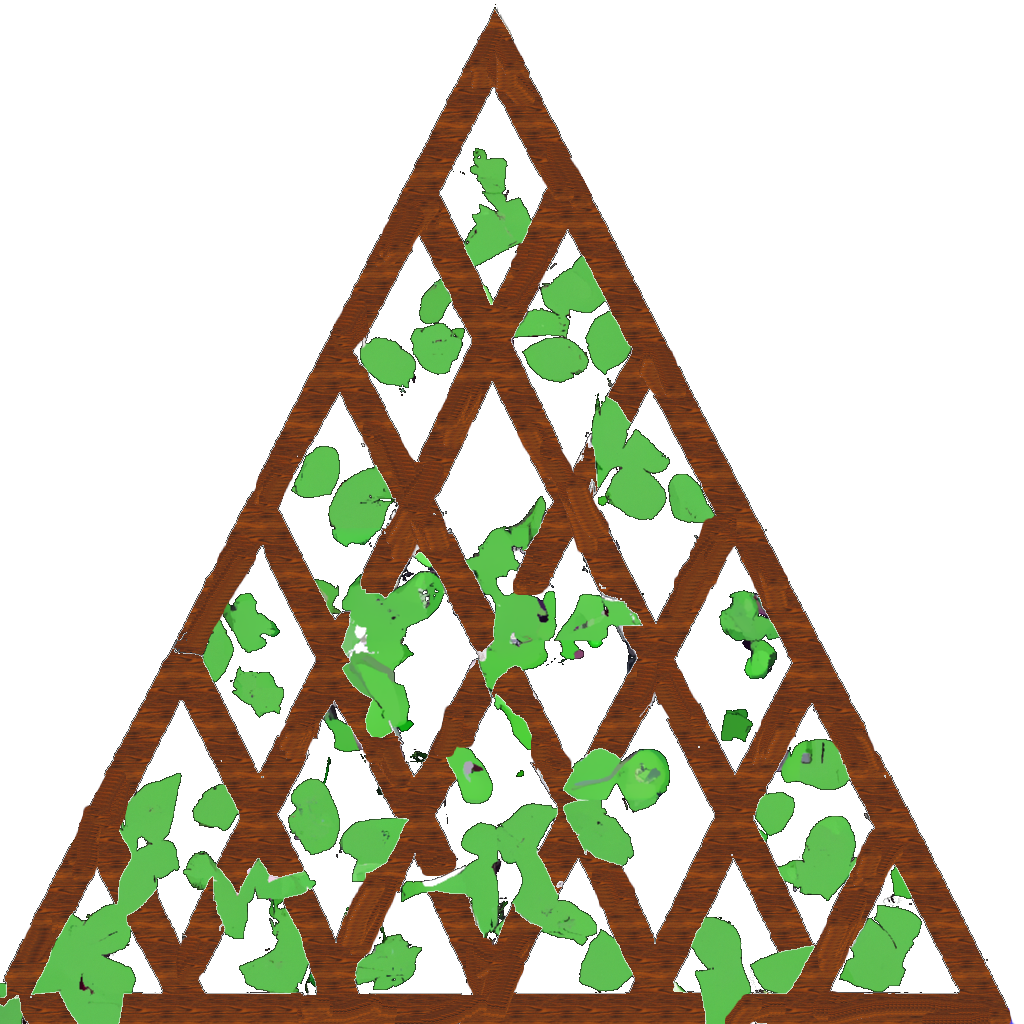
\includegraphics[width=0.17\textwidth]{../figures/trellis.png} & & 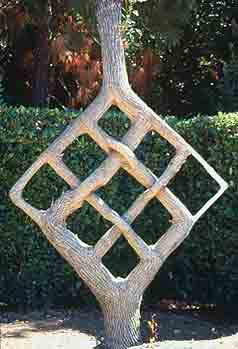
\includegraphics[width=0.12\textwidth]{../figures/grid_topiary.jpeg} & & 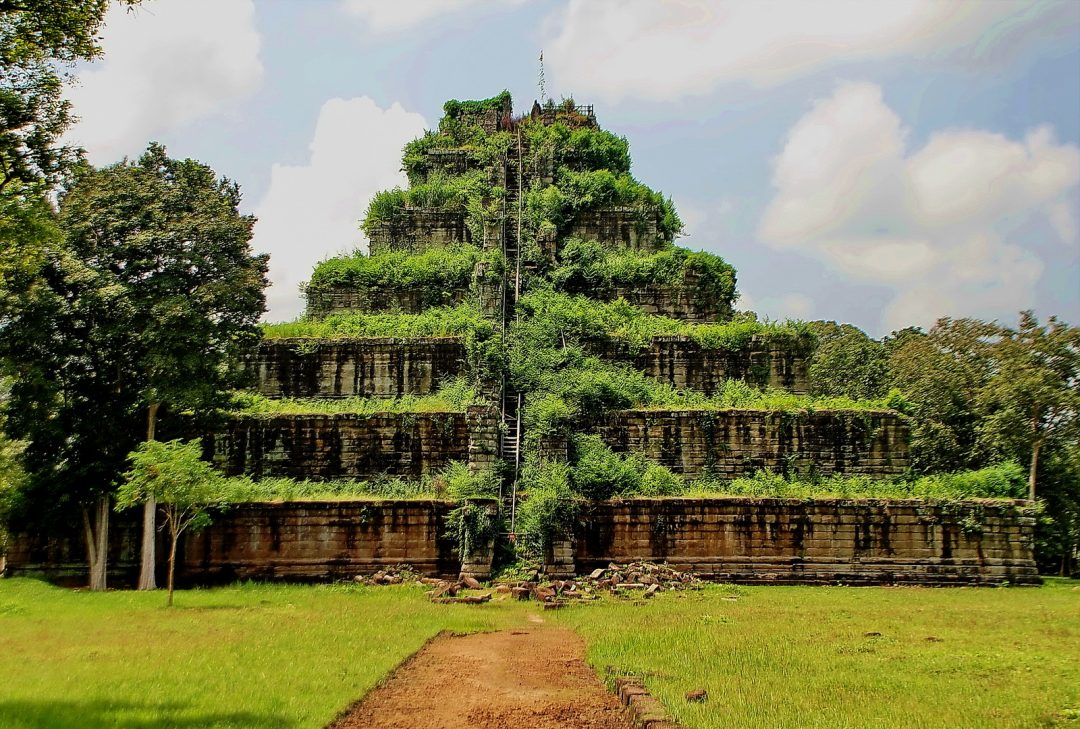
\includegraphics[width=0.23\textwidth]{../figures/tree_pyramid.jpeg} \\\\
      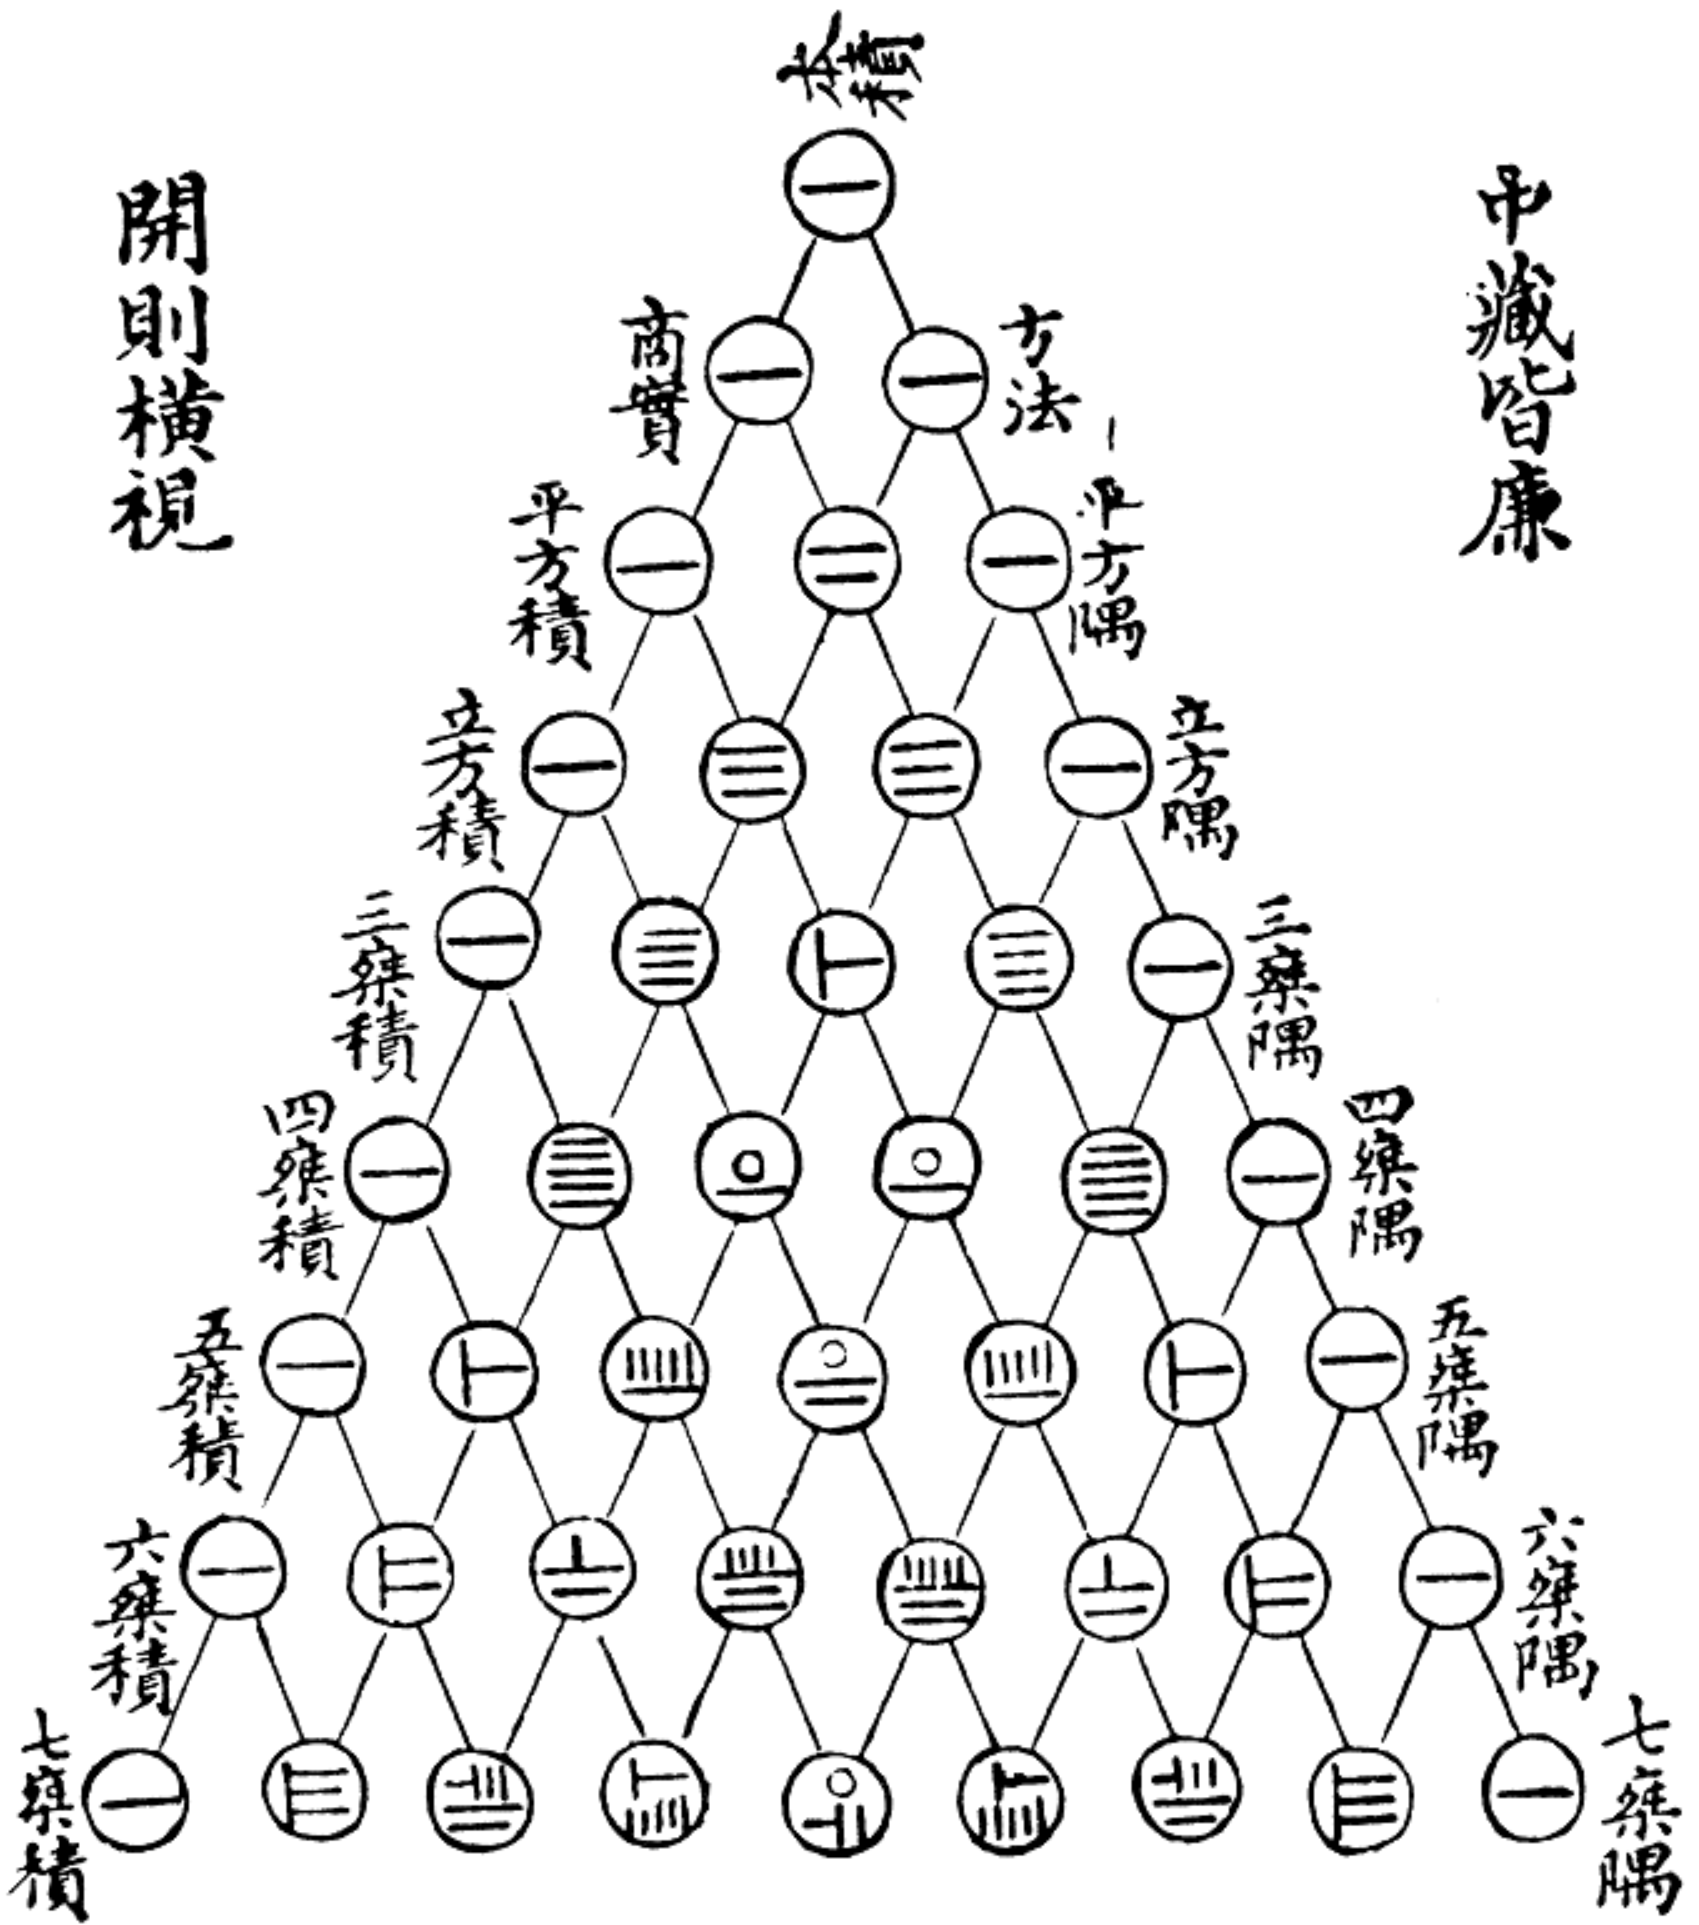
\includegraphics[width=0.17\textwidth]{../figures/jiaxian_triangle.png} & &
      \rotatebox{37}{\scalebox{0.9}{$
      \begin{pNiceMatrix}[nullify-dots,xdots/line-style=loosely dotted,delimiters-color=gray]
        \sigma_1^\shri & \Lambda & \Cdots & \Lambda^*_\sigma\\
                       & \Ddots  & \Ddots & \Vdots\\
                       &         &        & \Lambda\\
                       &         &        & \sigma_n^\shup \\
      \end{pNiceMatrix}$}} & & \scalebox{0.23}{\mkTrellis{9}}\\
      Jia Xian Triangle & & CYK Parsing & & Trellis Automaton\\
      Jia, $\sim$1030 A.D. & & Sakai, 1961 A.D. & & Dyer, 1980 A.D.\\
    \end{tabular}
  \end{center}
\end{frame}

\begin{frame}{A few observations on algebraic parsing}
  \begin{itemize}
    \item The matrix $\mathbf M^*$ is strictly upper triangular, i.e., nilpotent of degree $n$
    \item Recognizer can be translated into a parser by storing backpointers\\\\
  \end{itemize}\vspace{0.2cm}
  \begin{tabular}{ c c c }
    \small{$\mathbf{M}_1 = \mathbf{M}_0 + \mathbf{M}_0^2$} & \small{$\mathbf{M}_2 = \mathbf{M}_1 + \mathbf{M}_1^2$} & \small{$\mathbf{M}_3 = \mathbf{M}_2 + \mathbf{M}_2^2 = \mathbf{M}_4$} \\
    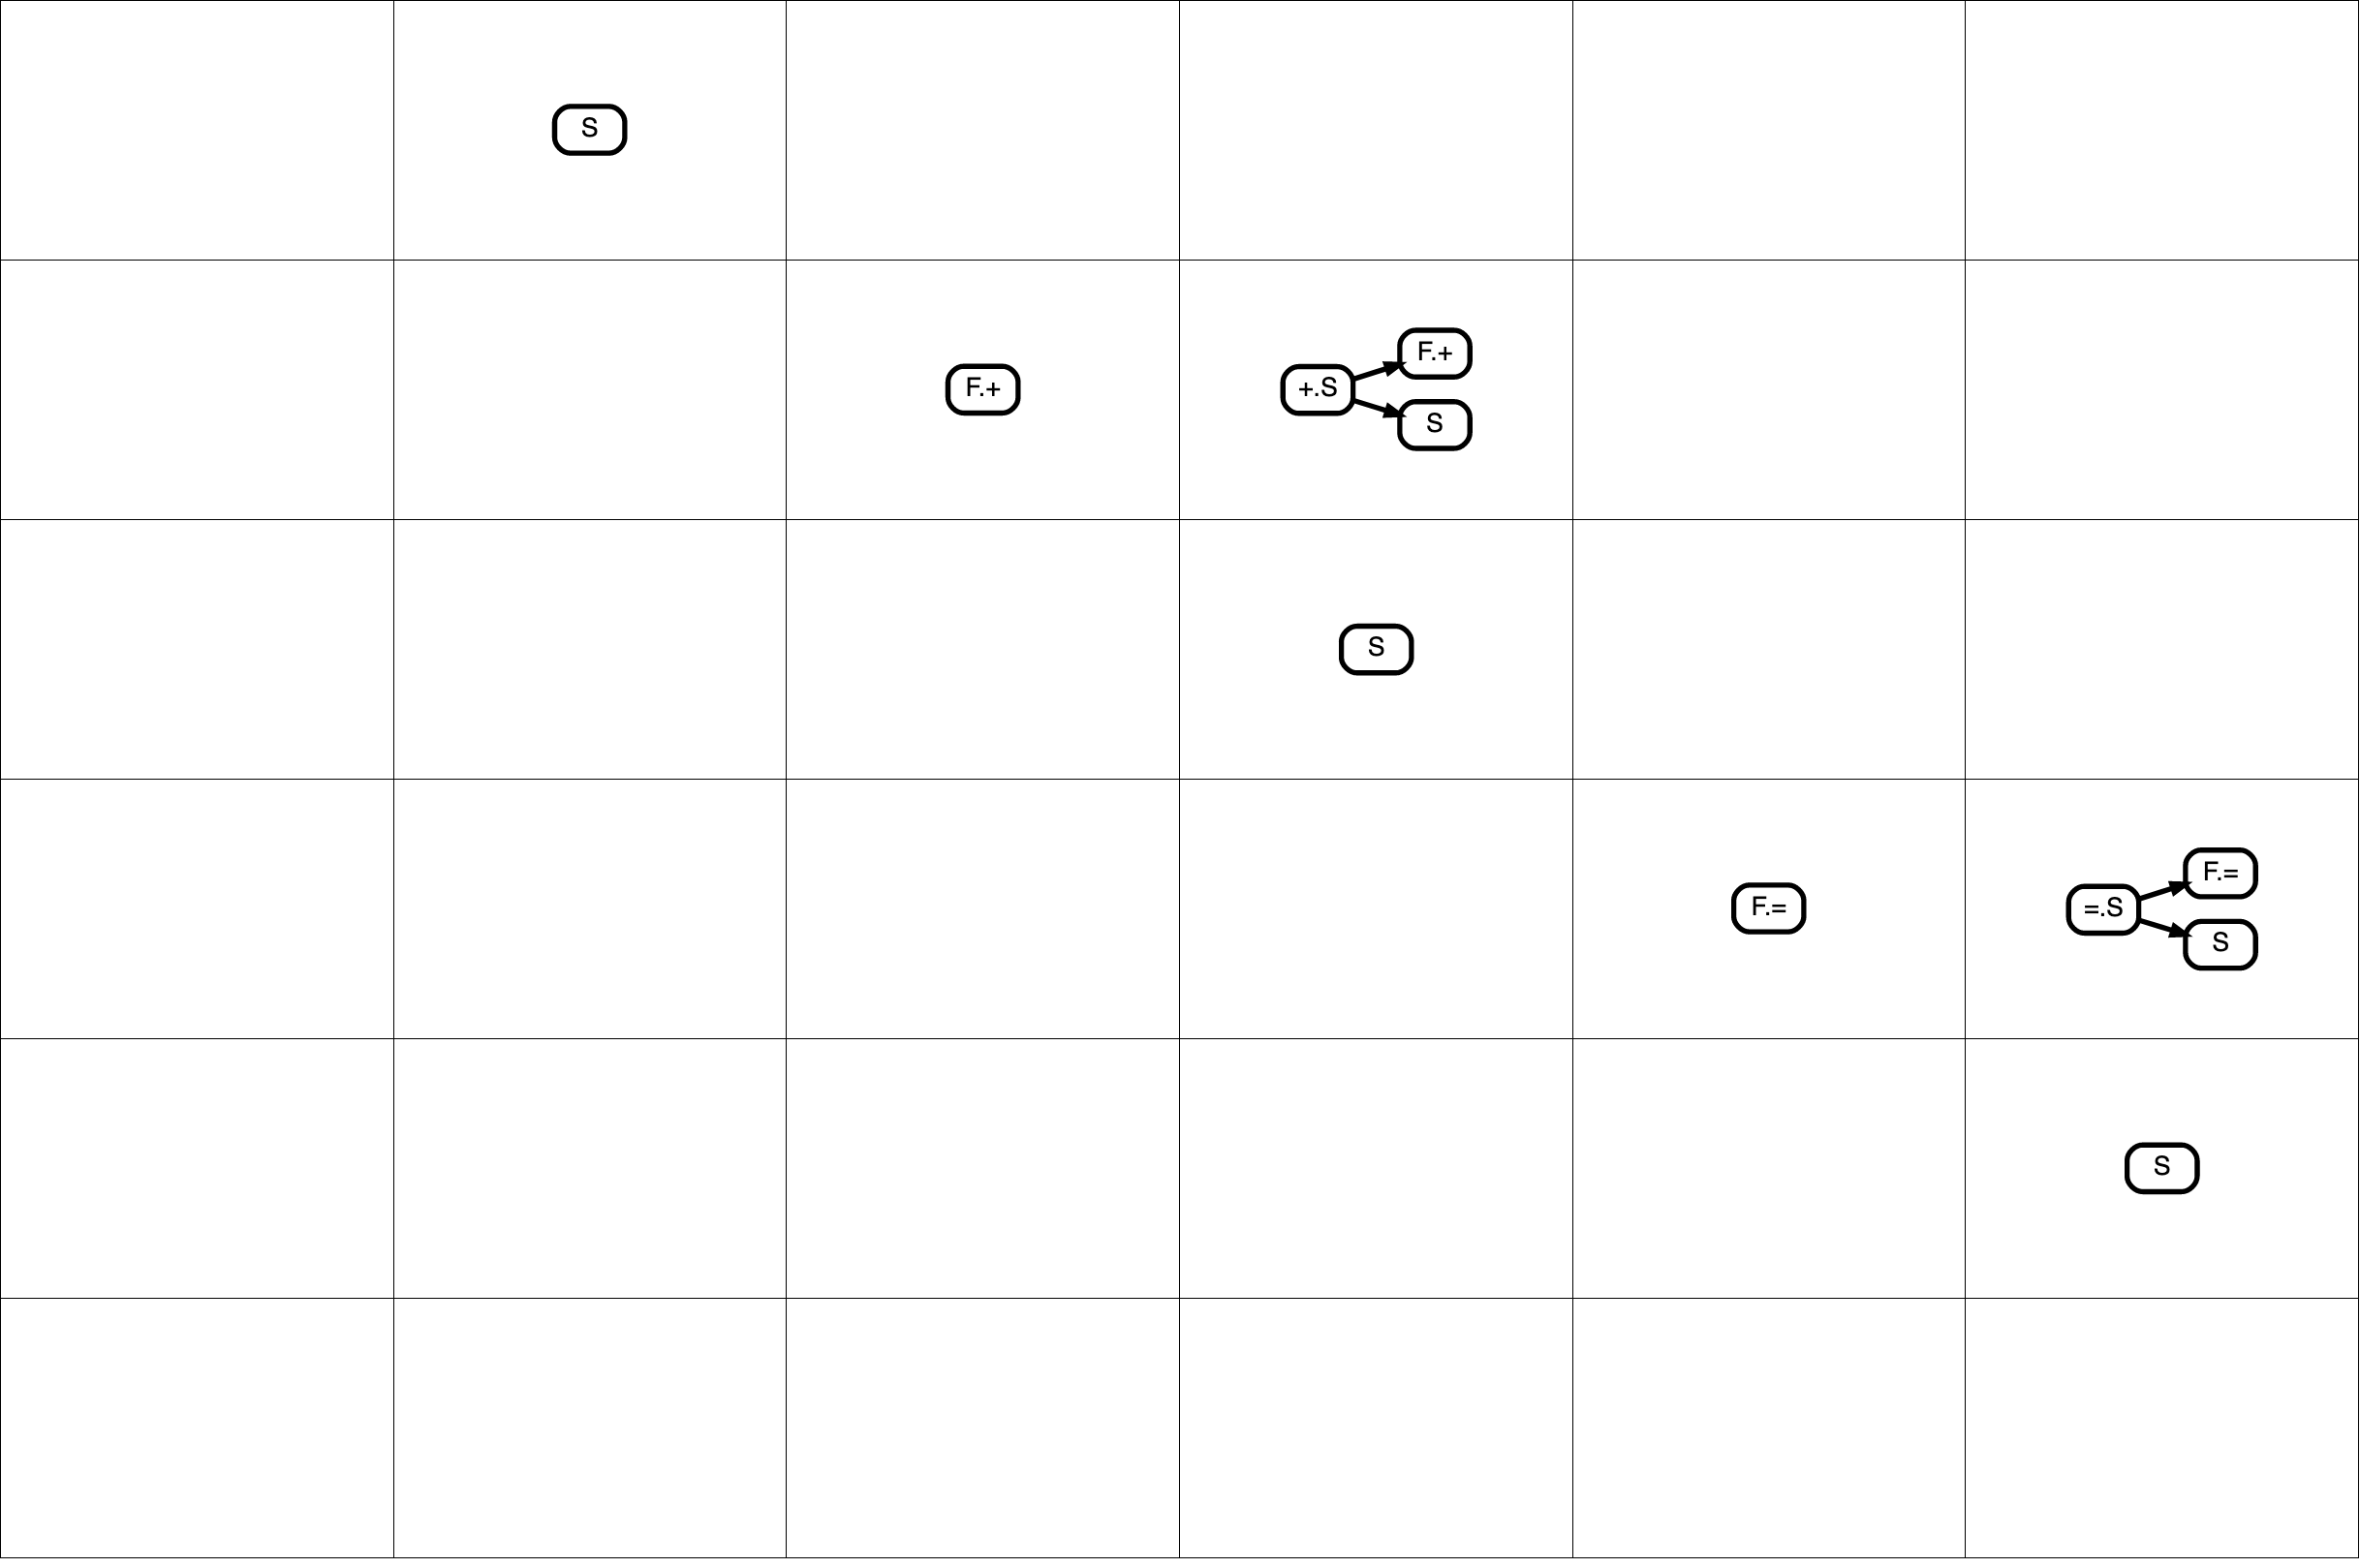
\includegraphics[trim=420 288 0 0,clip, width=3.6cm]{../figures/parse2.png} &
    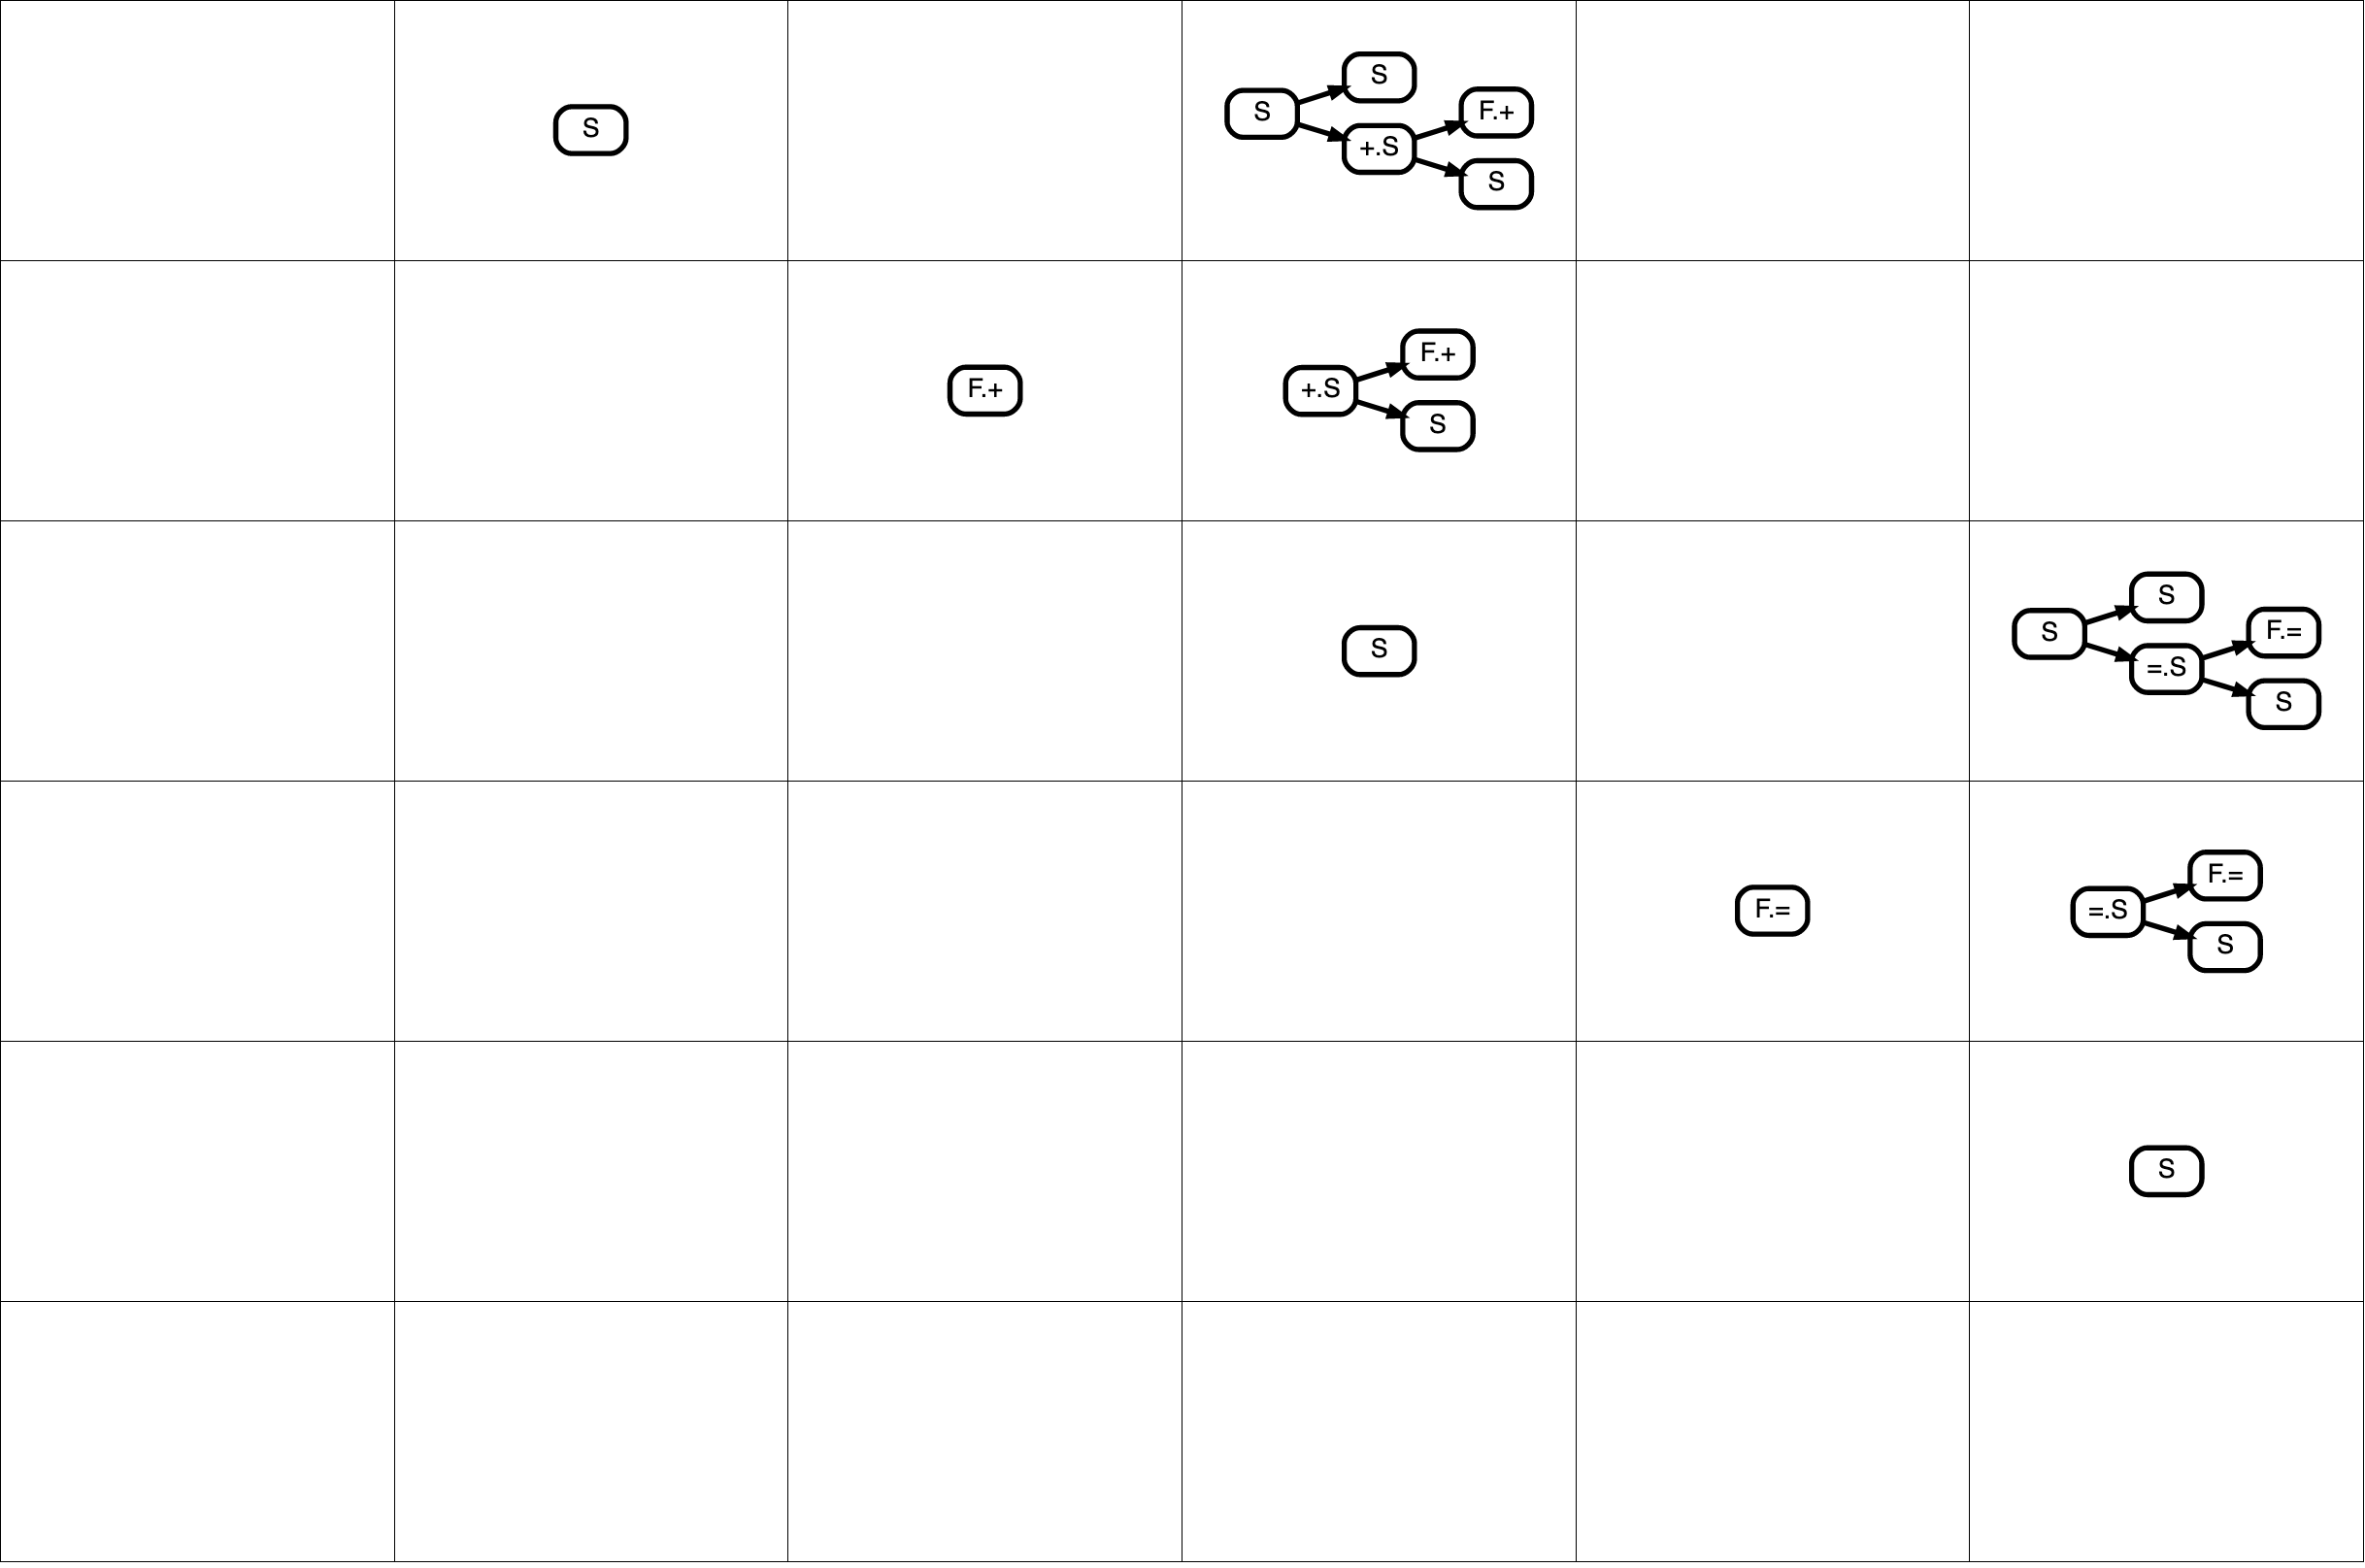
\includegraphics[trim=420 285 0 0,clip, width=3.6cm]{../figures/parse3.png} &
    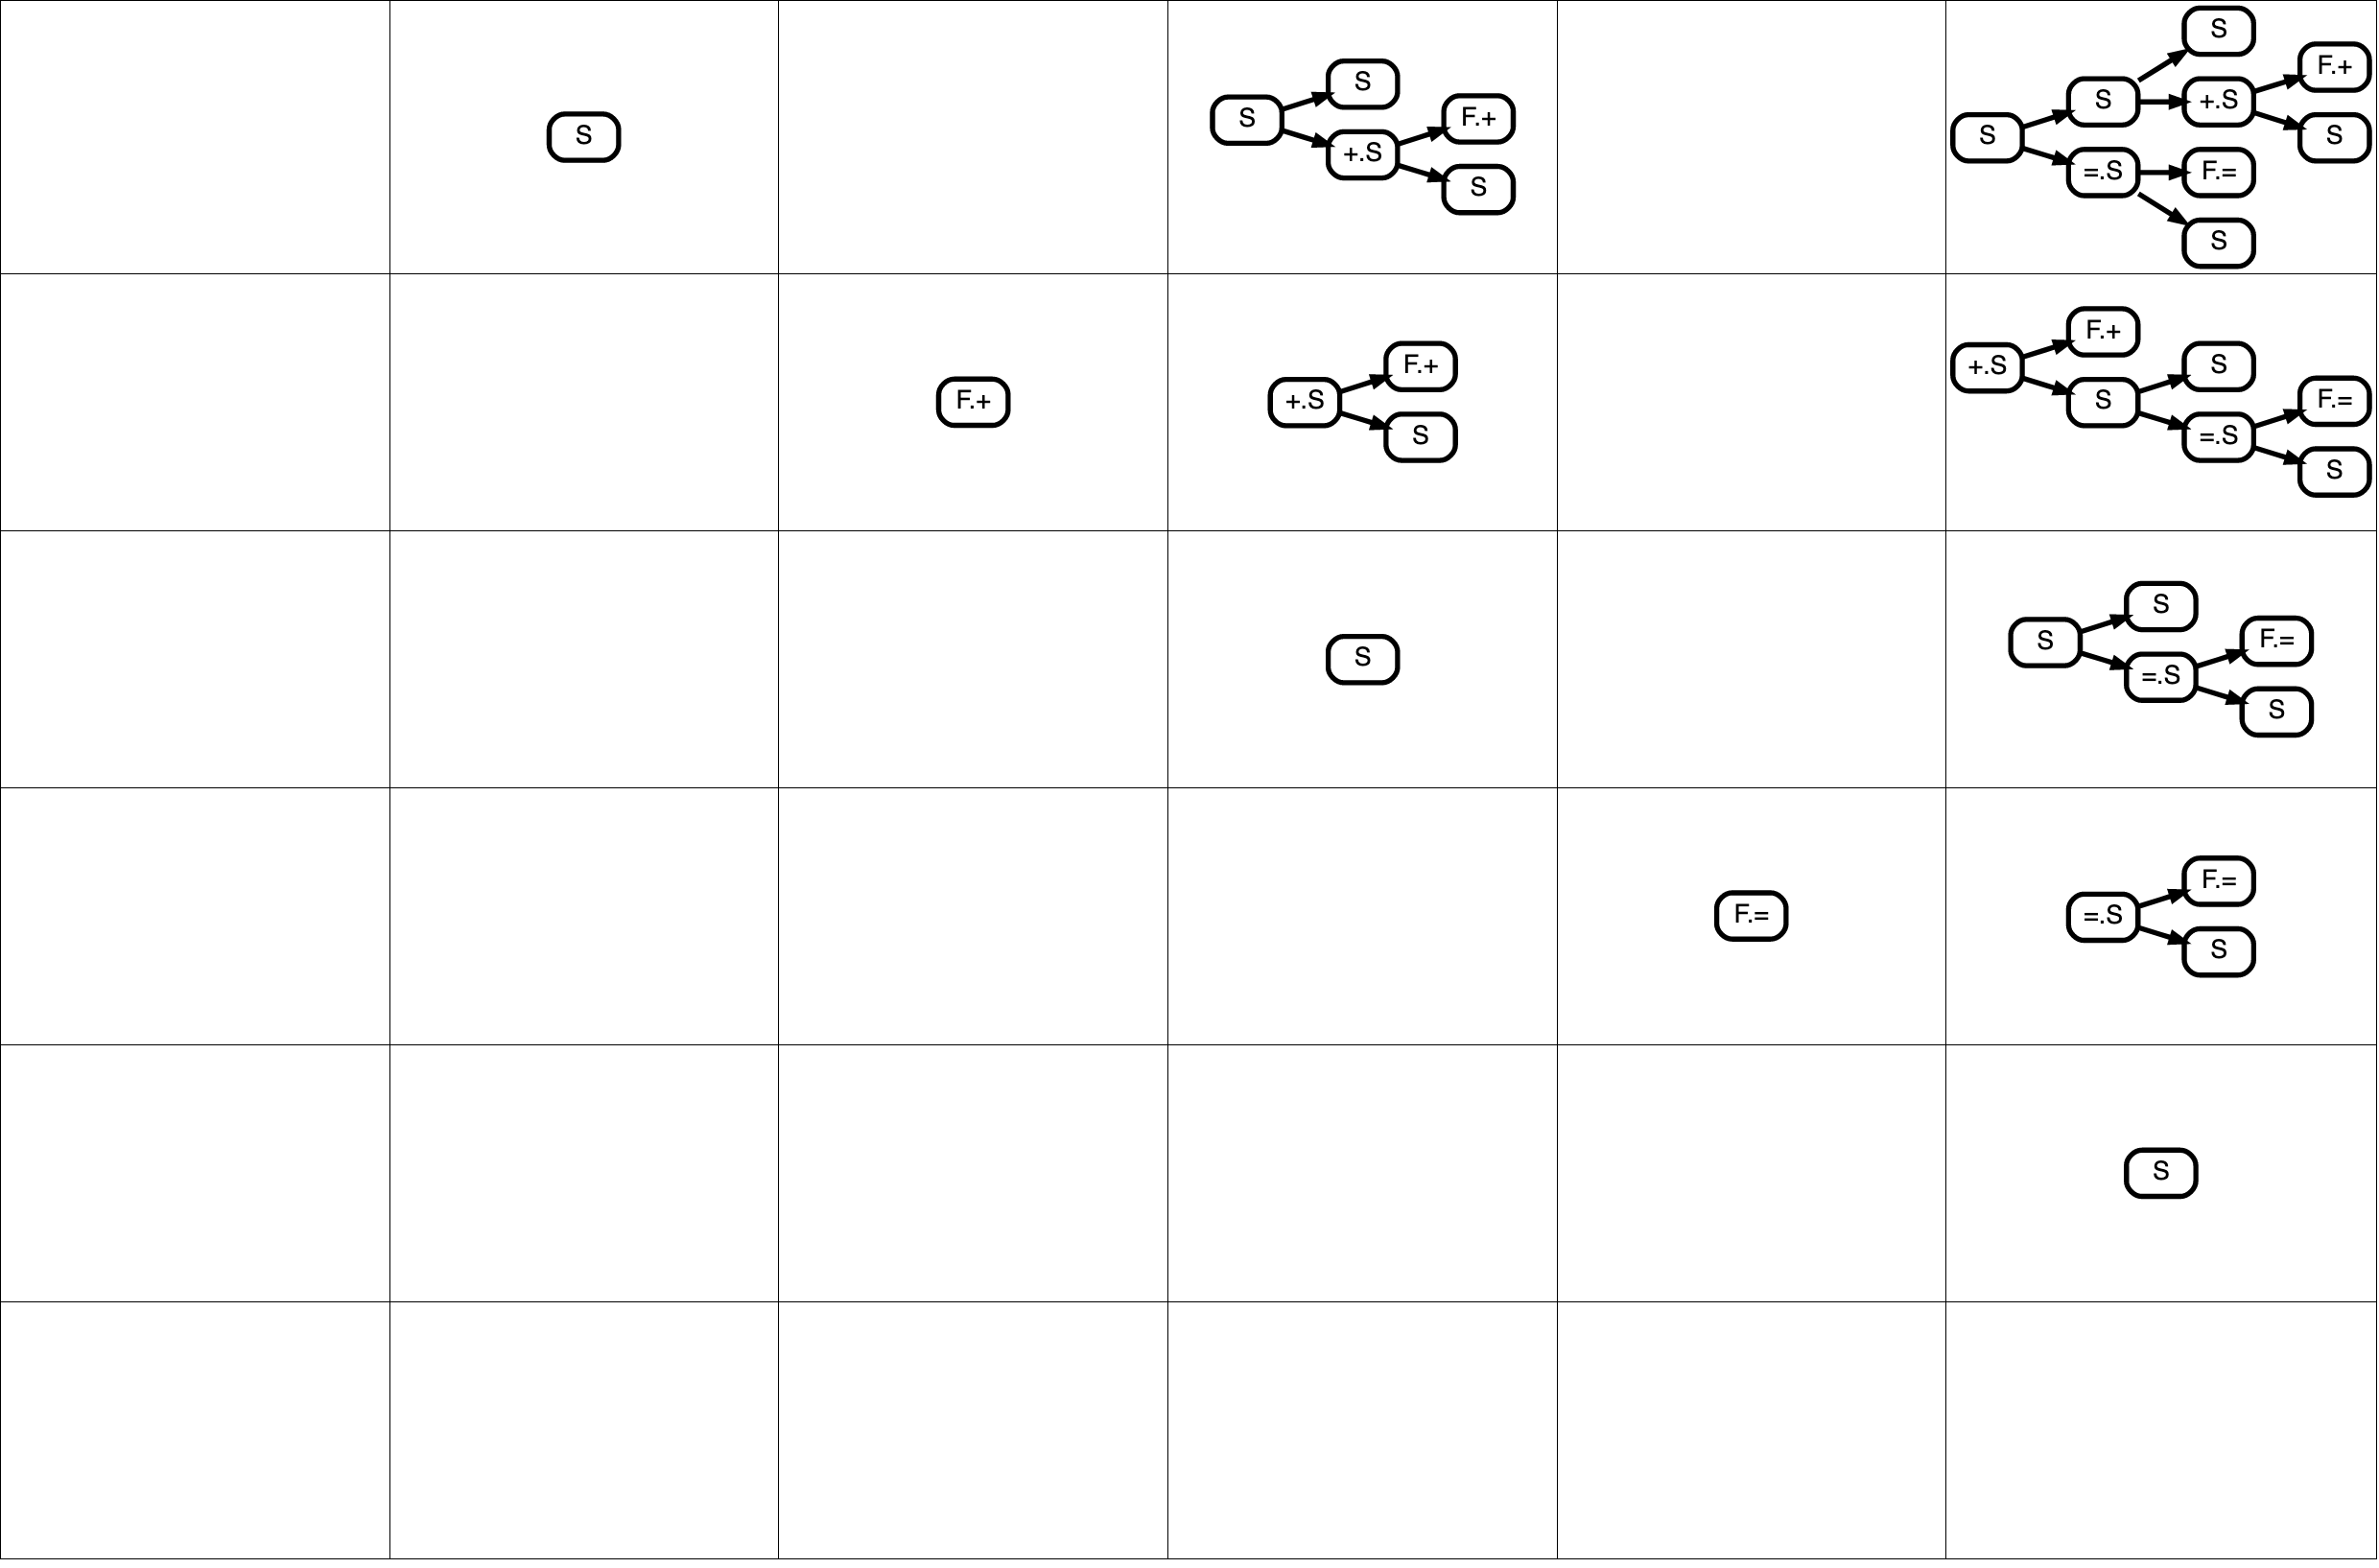
\includegraphics[trim=420 287 0 0,clip, width=3.63cm]{../figures/parse4.png}
  \end{tabular}
  \begin{itemize}
    \item The $\otimes$ operator is \textit{not} associative: $S \otimes (S \otimes S) \neq (S \otimes S) \otimes S$
    \item Built-in error recovery: nonempty submatrices = parsable fragments
    \item \texttt{seekFixpoint \{ it + it * it \}} is sufficient but unnecessary
    \item If we had a way to solve for $\mathbf{M = M + M}^2$ directly, power iteration would be unnecessary, could solve for $\mathbf{M = M}^2$ above superdiagonal
  \end{itemize}
\end{frame}

\begin{frame}[fragile]{Satisfiability + holes}
  \begin{itemize}
    \item Can be lowered onto a Boolean tensor $\mathbb{B}_2^{n\times n \times |V|}$ (Valiant, 1975)
    \item Binarized CYK parser can be efficiently compiled to a SAT solver
    \item Enables sketch-based synthesis in either $\sigma$ or $\mathcal G$: just use variables!
    \item We simply encode the characteristic function, i.e. $\mathds{1}_{\subseteq V}: V\rightarrow \mathbb{Z}_2^{|V|}$
    \item $\oplus, \otimes$ are defined as $\boxplus, \boxtimes$, so that the following diagram commutes:
    \[\begin{tikzcd}
        2^V \times 2^V \arrow[r, "\oplus/\otimes"] \arrow[d, "\mathds{1}^2"]
        & 2^V \arrow[d, "\mathds{1}\phantom{^{-1}}"] \\
        \mathbb{Z}_2^{|V|} \times \mathbb{Z}_2^{|V|} \arrow[r, "\boxplus/\boxtimes", labels=below] \arrow[u, "\mathds{1}^{-2}"]
        & \mathbb{Z}_2^{|V|} \arrow[u, "\mathds{1}^{-1}"]
    \end{tikzcd}\]
    \item These operators can be lifted into matrices/tensors in the usual way
    \item In most cases, only a few nonterminals are active at any given time
%    \item More sophisticated representations are known for $\binom{n}{0 \leq k}$ subsets
%    \item If density is desired, possible to use the Maculay representation
%            \item Set joins are an active topic of research in SQL query optimization
  \end{itemize}
\end{frame}

\begin{frame}[fragile]{Satisfiability + holes}
  Let us consider an example with two holes, $\sigma = 1$ \hole\phantom{.}\hole, and the grammar being $G\coloneqq\{S\rightarrow N O N, O \rightarrow + \mid \times, N \rightarrow 0 \mid 1\}$. This can be rewritten into CNF as $G'\coloneqq \{S \rightarrow N L, N \rightarrow 0 \mid 1, O \rightarrow × \mid +, L \rightarrow O N\}$. Using the algebra where $\oplus=\cup$, $X \otimes Z = \big\{\;w \mid \langle x, z\rangle \in X \times Z, (w\rightarrow xz) \in P\;\big\}$, the fixpoint $M' = M + M^2$ can be computed as follows:\\\vspace{10pt}

  \resizebox{\textwidth}{!}{
{\renewcommand{\arraystretch}{1.2}
\noindent\phantom{...}\begin{tabular}{|c|c|c|c|}
  \hline
  & $2^V$ & $\mathbb{Z}_2^{|V|}$ & $\mathbb{Z}_2^{|V|}\rightarrow\mathbb{Z}_2^{|V|}$\\\hline
  $M_0$ & \begin{pmatrix}
  \phantom{V} & \tiny{\{N\}} &         &             \\
              &              & \{N,O\} &             \\
              &              &         & \{N,O\} \\
              &              &         &
  \end{pmatrix} & \begin{pmatrix}
  \phantom{V} & \ws\bs\ws\ws &              &              \\
              &              & \ws\bs\bs\ws &              \\
              &              &              & \ws\bs\bs\ws \\
              &              &              &
  \end{pmatrix} & \begin{pmatrix}
     \phantom{V} & V_{0, 1} &          &          \\
                 &          & V_{1, 2} &          \\
                 &          &          & V_{2, 3} \\
                 &          &          &
  \end{pmatrix} \\\hline
  $M_1$ & \begin{pmatrix}
  \phantom{V} & \tiny{\{N\}} & \varnothing &         \\
              &              & \{N,O\}     & \{L\}   \\
              &              &             & \{N,O\} \\
              &              &             &
  \end{pmatrix} & \begin{pmatrix}
  \phantom{V} & \ws\bs\ws\ws & \ws\ws\ws\ws &              \\
              &              & \ws\bs\bs\ws & \bs\ws\ws\ws \\
              &              &              & \ws\bs\bs\ws \\
              &              &              &
  \end{pmatrix} & \begin{pmatrix}
                   \phantom{V} & V_{0, 1} & V_{0, 2} &          \\
                   &          & V_{1, 2} & V_{1, 3} \\
                   &          &          & V_{2, 3} \\
                   &          &          &
  \end{pmatrix} \\\hline
  $M_\infty$ & \begin{pmatrix}
  \phantom{V} & \tiny{\{N\}} & \varnothing & \{S\}   \\
              &              & \{N,O\}     & \{L\}   \\
              &              &             & \{N,O\} \\
              &              &             &
  \end{pmatrix} & \begin{pmatrix}
  \phantom{V} & \ws\bs\ws\ws & \ws\ws\ws\ws & \ws\ws\ws\bs \\
              &              & \ws\bs\bs\ws & \bs\ws\ws\ws \\
              &              &              & \ws\bs\bs\ws \\
              &              &              &
  \end{pmatrix} & \begin{pmatrix}
                   \phantom{V} & V_{0, 1} & V_{0, 2} & V_{0, 3} \\
                   &          & V_{1, 2} & V_{1, 3} \\
                   &          &          & V_{2, 3} \\
                   &          &          &
  \end{pmatrix}\\\hline
\end{tabular}
}
  }
\end{frame}

\begin{frame}[fragile]{Semiring algebras: Part I}
  The prior solution tell us whether $A(\sigma)$ is nonempty, but forgets the solution(s). To solve for $A(\sigma)$, a na\"ive approach accumulates a mapping of nonterminals to sets of strings. Letting $D = V \rightarrow \mathcal{P}(\Sigma^*)$, we define $\oplus, \otimes: D \times D \rightarrow D$. Initially, we construct $M_0[r+1=c] = p(\sigma_r)$ using:

  \begin{equation*}
    p(s: \Sigma) \mapsto \{w \mid (w \rightarrow s)\in P\} \text{ and } p(\hole) \mapsto \bigcup_{s\in \Sigma} p(s)
  \end{equation*}

  $p(\cdot)$ constructs the superdiagonal, then we solve for $\Lambda_\sigma^*$ using the algebra:

  \begin{equation*}
    X \oplus Z \mapsto \big\{w \stackrel{+}{\Rightarrow} (X \circ w) \cup (Z \circ w) \mid w \in \pi_1(X \cup Z)\big\}
  \end{equation*}

  \begin{equation*}
    X \otimes Z \mapsto \bigoplus_{w, x, z}\big\{w \stackrel{+}{\Rightarrow} (X\circ x)(Z\circ z) \mid (w\rightarrow xz) \in P, x\in X, z\in Z\big\}
  \end{equation*}

  \noindent After $M_\infty$ is attained, the solutions can be read off via $\Lambda_\sigma^* \circ S$. The issue here is exponential growth when eagerly computing the transitive closure.
\end{frame}

\begin{frame}[fragile]{Semiring algebras: Part II}
  The prior encoding can be improved using an ADT $\mathbb{T}_3 = (V \cup \Sigma) \rightharpoonup \mathbb{T}_2$ where $\mathbb{T}_2 = (V \cup \Sigma) \times (\mathbb{N} \rightharpoonup \mathbb{T}_2\times\mathbb{T}_2)$. We construct $\hat\sigma_r = \dot{p}(\sigma_r)$ using:

  \begin{equation*}
    \dot{p}(s: \Sigma) \mapsto \Big\{\mathbb{T}_2\big(w, \big[\langle\mathbb{T}_2(s), \mathbb{T}_2(\varepsilon)\rangle\big]\big) \mid (w \rightarrow s)\in P\Big\} \text{ and } \dot{p}(\hole) \mapsto \bigoplus_{s\in \Sigma} p(s)
  \end{equation*}

  \noindent We then compute the fixpoint $M_\infty$ by redefining $\oplus, \otimes: \mathbb{T}_3 \times \mathbb{T}_3 \rightarrow \mathbb{T}_3$ as:

  \begin{equation*}
    X \oplus Z \mapsto \bigcup_{\mathclap{k\in \pi_1(X \cup Z)}}\Big\{k \Rightarrow \mathbb{T}_2(k, x \cup z) \mid x \in \pi_2(X\circ k), z \in \pi_2(Z\circ k)\Big\}
  \end{equation*}

  \begin{equation*}
    X \otimes Z \mapsto \bigoplus_{\mathclap{(w\rightarrow xz) \in P}}\Big\{\mathbb{T}_2\big(w, \big[\langle X\circ x, Z\circ z\rangle\big]\big) \mid x \in \pi_1(X), z \in \pi_1(Z)\Big\}
  \end{equation*}
\end{frame}

\begin{frame}[fragile]{Semiring algebras: Part III}
  \begin{equation*}
    \hspace{-3cm}L(p) = 1 + p L(p) \phantom{space} P(a) = \Sigma + V + V L\big(V^2P(a)^2\big)
  \end{equation*}
  \vspace{-1cm}\begin{figure}[H]
                 \resizebox{0.9\columnwidth}{!}{
                   \begin{tikzpicture}
                   [
                     grow                    = right,
                     sibling distance        = 3em,
                     level distance          = 5em,
                     edge from parent/.style = {draw, -latex},
                     every node/.style       = {font=\footnotesize},
                     sloped
                   ]
                     \node [root] {S}
                     child { node [env] {BC}
                     child { node [root] {B}
                     child { node [env] {RD}
                     child { node [root] {R} edge from parent node [above] }
                     child { node [root] {D} edge from parent node [above] }
                     edge from parent node [above] }
                     edge from parent node [below] }
                     child { node [root] {C}
                     child { node [env] {\ldots\vphantom{BB}} edge from parent node [below] }
%  child { edge from parent node [above] {\ldots} }
                     edge from parent node [below] }
                     edge from parent node [above] }
                     child { node [env] {\ldots\vphantom{BB}} edge from parent node [below] }
                     child { node [env] {AB}
                     child { node [root] {A}
                     child {
                       node [env] {QC}
                       child { node [root] {Q} edge from parent node [above] }
                       child { node [root] {C} edge from parent node [above] }
                       edge from parent node [above]
                     }
%    child { node [env] {ZQ} edge from parent node [above] }
                     child { node [env] {\ldots\vphantom{BB}} edge from parent node [below] }
                     edge from parent node [below] }
                     child { node [root] {B}
                     child { node [env] {RD}
                     child { node [root] {R} edge from parent node [above] }
                     child { node [root] {D} edge from parent node [above] }
                     edge from parent node [above] }
                     edge from parent node [below] }
                     edge from parent node [above] };
                   \end{tikzpicture}
                 }
                 \vspace{-0.5cm}\caption{A partial $\mathbb{T}_2$ for the grammar with productions $P=\{S \rightarrow BC \mid \ldots \mid AB, B\rightarrow RD \mid \ldots, A\rightarrow QC \mid \ldots\}$.}
  \end{figure}
\end{frame}

\begin{frame}[fragile]{Sampling trees with replacement}
  Given a probabilistic CFG whose productions indexed by each nonterminal are decorated with a probability vector $\mathbf{p}$ (this may be uniform in the non-probabilistic case), we define a tree sampler $\Gamma: \mathbb{T}_2 \rightsquigarrow \mathbb{T}$ which recursively samples children according to a Multinoulli distribution:

  \begin{equation*}
    \Gamma(T) \mapsto \begin{cases}
      \text{Multi} \big(\texttt{children}(T), \mathbf{p}\big) & \text{ if $T$ is a \texttt{root}} \\
      \big\langle \Gamma\big(\pi_1(T)\big), \Gamma\big(\pi_2(T)\big) \big\rangle & \text{ if $T$ is a \texttt{child} }
    \end{cases}
  \end{equation*}

  This is closely related to the generating function for the ordinary Boltzmann sampler from analytic combinatorics,

  \begin{equation*}
    \Gamma C(x) \mapsto \begin{cases}
                          \text{Bern} \left(\frac{A(x)}{A(x) + B(x)}\right) \rightarrow \Gamma A(x) \mid \Gamma B(x) & \text{ if } \mathcal{C}=\mathcal{A}+\mathcal{B} \\
                          \big\langle \Gamma A(x), \Gamma B(x)\big\rangle & \text{ if } \mathcal{C}=\mathcal{A} \times \mathcal{B}
    \end{cases}
  \end{equation*}

  \noindent however unlike Duchon et al. (2004), rejection is unnecessary to ensure exact-size sampling, as all trees in $\mathbb{T}_2$ will necessarily be the same size.
\end{frame}

\begin{frame}[fragile]{A pairing function for replacement-free tree sampling}
  The total number of trees induced by a given sketch template is given by:

  \begin{equation*}
    |T: \mathbb{T}_2| \mapsto \begin{cases}
%    \big|\{s \mid \big(\texttt{root}(T) \rightarrow s\big) \in P_\cap\}\big| & \text{if $T$ is a leaf,} \\
                                1  & \text{if $T$ is a leaf,} \\
                                \sum_{\langle T_1, T_2\rangle \in \texttt{children}(T)} |T_1| \cdot |T_2| & \text{otherwise.}
    \end{cases}
  \end{equation*}\\

  To sample from $\mathbb{T}_2$ without replacement, we define a pairing function:

% Small text
\begin{footnotesize}
  \begin{equation*}
  \varphi(T: \mathbb{T}_2, i: \mathbb{Z}_{|T|}) \mapsto \begin{cases}
  \texttt{BTree}\big(\texttt{root}(T)\big) & \text{if $T$ is a leaf,} \vspace{5pt}\\
  \textbf{let } r = |\texttt{children}(T)|,\\
  \phantom{\textbf{Let }} F(n) = \sum_{\langle l, r\rangle \in \texttt{children}[0 \ldots n]}}|l|\cdot|r|,\\
  \phantom{\textbf{Let }} F^{-1}(u)=\inf \big\{x \mid u \leq F(x)\big\},\\
  \phantom{\textbf{Let }} q=i - F\big(F^{-1}(i)\big),\\
  \phantom{\textbf{Let }} l, r = \texttt{children}[t],\\
  \phantom{\textbf{Let }} q_1, q_2 =\big\langle\lfloor\frac{q}{|r|}\rfloor, q \pmod{|r|}\big\rangle,\\
  \phantom{\textbf{Let }} T_1, T_2 = \big\langle\varphi(l, q_1), \varphi(r, q_2)\big\rangle \textbf{ in } \\
  \texttt{BTree}\big(\texttt{root}(T), T_1, T_2\big) & \text{otherwise.} \\
  \end{cases}
  \end{equation*}
\end{footnotesize}
\end{frame}

\begin{frame}[fragile]{Enumerative search with reranking}
Given $\sigma: \Sigma^*$, let $P_\theta(\sigma) = \prod_{i=1}^{|\sigma|}P_\theta(\sigma_i \mid \sigma_{i-1}\ldots\sigma_{i-n})$. This defines an ordering over $\Sigma^*$. Then, for each retrieved set $\sigma \in \hat{a} \subseteq A$ drawn before timeout, we score the repair and return $\hat{A}$ in ascending order:

\begin{algorithm}[H]
\caption{Enumerative tree sampling with n-gram reranking}
\label{alg:enum_ngram}
\begin{algorithmic}[1]
\Require $T: \mathbb{T}_2$ intersection grammar, $P_\theta: \Sigma^d \rightarrow \mathbb{R}$ Markov chain
\State $\hat{A} \gets \varnothing, \texttt{seed} \gets 0$ \Comment{Initialize set of repairs.}
%\State $[\mathcal{T, P}]\texttt{.comparator} = \lambda\langle\sigma, q, \gamma\rangle.(\frac{\gamma}{|\sigma|})$
\For{$\texttt{seed} < |T|$ and uninterrupted}
\State $t \gets \varphi'(T, \texttt{seed++})}$ \Comment{Decode fresh tree and add.}
\State $\hat{A} \gets \hat{A} \cup \{\text{\textleaf}(t)\}$
%\Until{interrupted or $\texttt{seed} = |T|$.}
\EndFor
\State \Return $[\sigma \in \hat{A} \textbf{ ranked by } \text{NLL}(\sigma)]$ \Comment{Rerank by n-gram likelihood.}
\end{algorithmic}
\end{algorithm}

The issue is, the bijection is defined over labeled binary trees and does not guarantee unique strings, as the CFG may be ambiguous. In practice, this matters if we care about $\mathcal{O}(n)$ convergence!
\end{frame}

\begin{frame}[fragile]{Potential ambiguity of Levenshtein-Bar-Hillel grammars}
The previous technique enumerates parse trees in a given $\mathbb{T}_2$, but does not guarantee string uniqueness since the CFG may be ambiguous.

\begin{lemma}\label{lemma:ambiguity}
If the FSA, $\alpha$, is ambiguous, the intersection CFG, $G_\cap$, can be ambiguous.
\end{lemma}

\begin{proof}
Let $\ell$ be the language defined by $G=\{S\rightarrow LR, L \rightarrow\texttt{(}, R \rightarrow\texttt{)}\}$, where $\alpha=L(\err\sigma, 2)$, the broken string $\err\sigma$ is $\texttt{)(}$, and $\mathcal{L}(G_\cap) = \ell \cap \mathcal{L}(\alpha)$. Then, $\mathcal{L}(G_\cap)$ contains the following two identical repairs: \texttt{\hlred{)}(\hlgreen{)}} with the parse $S \rightarrow q_{00}Lq_{21}\phantom{.}q_{21}Rq_{22}$, and \texttt{\hlorange{(}\hlorange{)}} with the parse $S \rightarrow q_{00}Lq_{11}\phantom{.}q_{11}Rq_{22}$.
\end{proof}

We can eliminate ambiguity and thereby improve the rate of convergence for natural syntax repair by first translating $\mathbb{T}_2$ into an FSA.
\end{frame}

\begin{frame}[fragile]{Existence of an FSA that generates $\mathcal{L}(G_\cap)$}
There is an FSA generating $\mathcal{L}(G_\cap)$. We first show this non-constructively:

\begin{lemma}\label{lemma:upper-bound}
The intersection grammar, $G_\cap$, is acyclic.
\end{lemma}

\begin{proof}
Assume $G_\cap$ is cyclic. Then $\mathcal{L}(G_\cap)$ must be infinite. But since $G_\cap$ generates $\ell \cap \mathcal{L}(\alpha)$ by construction and $\alpha$ is acyclic, $\mathcal{L}(G_\cap)$ is necessarily finite. Therefore, $G_\cap$ must not be cyclic.
\end{proof}

Since $G_\cap$ is acyclic and thus finite, it must be representable as an FSA. Using an FSA for decoding has many advantages, notably, it can be efficiently minimized and decoded in order of n-gram likelihood using a Markov chain or standard pretrained autoregressive language model.
\end{frame}

\begin{frame}[fragile]{Translating from $T_2$ to a DFA}
Let $+, *: \mathcal{A}\times \mathcal{A} \rightarrow \mathcal{A}$ be automata operators satisfying the property $\mathcal{L}(A_1 + A_2) = \mathcal{L}(A_1)\cup\mathcal{L}(A_2)$, and $\mathcal{L}(A_1 * A_2) = \mathcal{L}(A_1)\times\mathcal{L}(A_2)$. We can translate $\mathbb{T}_2$ to $\mathcal{A}$, as follows, recalling FSAs are closed over $+, *$:

\begin{equation*}
\mathcal{Y}(T:\mathbb{T}_2) \mapsto \begin{cases}
\alpha \mid \mathcal{L}(\alpha) = \{T\} & T: \Sigma, \\
\sum_{\langle T_1, T_2\rangle \in \texttt{children}(T)} \mathcal{Y}(T_1)*\mathcal{Y}(T_2) & T: VL\big(V^2P(a)^2\big)
\end{cases}
\end{equation*}
%
In the case of LBH intersections, $\mathcal{Y}(G_\cap')$ yields $\alpha: \mathcal{A} \mid \mathcal{L}(\alpha) = \ell\cap L(\err\sigma, d)$, which can be minimized via Brzozowski's algorithm then decoded:

\begin{figure}[H]
\centering
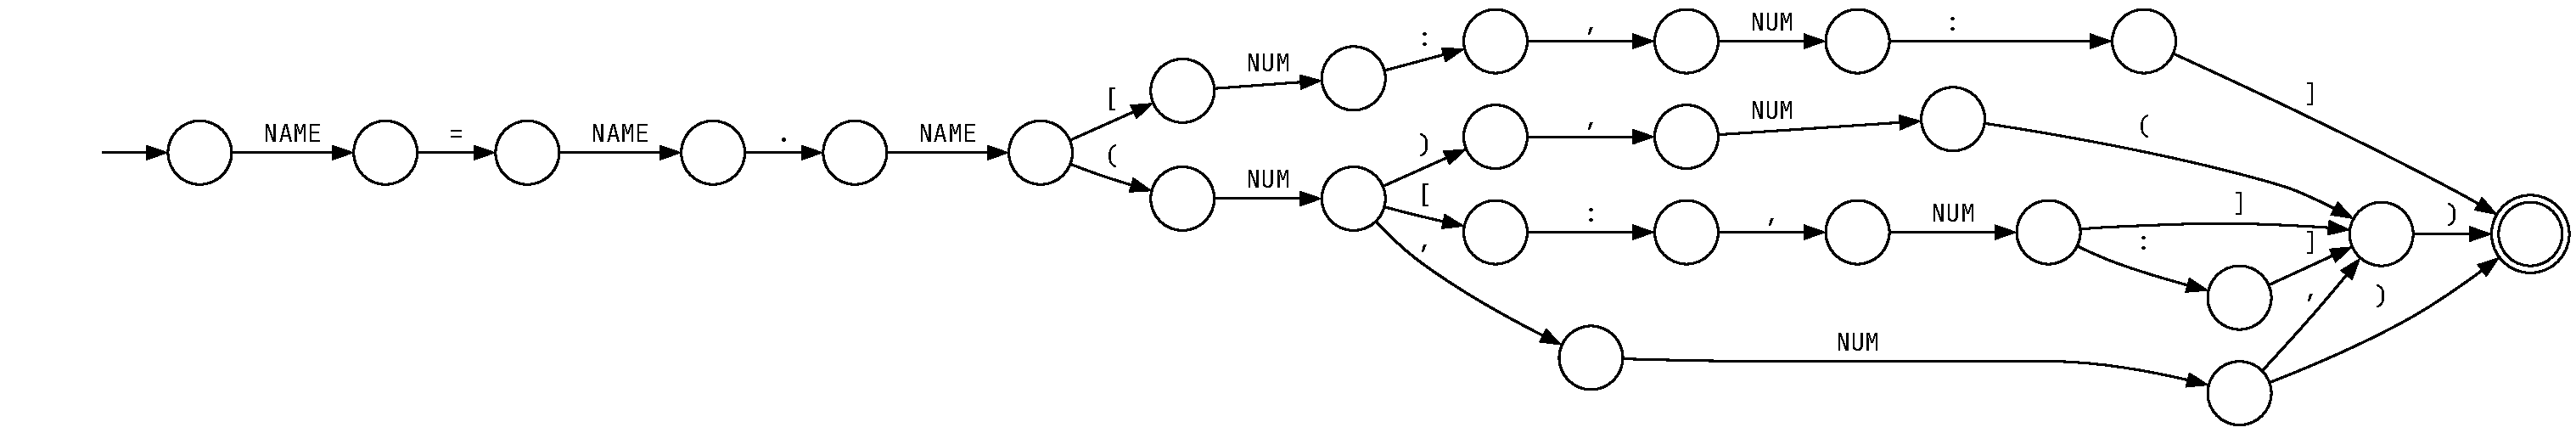
\includegraphics[width=0.9\textwidth]{../popl2025/exampleDFA.pdf}
\caption{$L(\scriptsize{\texttt{NAME = NAME . NAME ( NUM : , NUM : )}}, 2) \cap \ell_\textsc{Python}$}
\label{fig:exampleDFA}
\end{figure}
\end{frame}

\begin{frame}[fragile]{Decoding the DFA in order of normalized log likelihood}
\vspace{-0.3cm}
\begin{algorithm}[H]
\caption{Steerable DFA walk}
\label{alg:adaptive}
\begin{algorithmic}[1]
\Require $\mathcal{A} = \langle Q, \Sigma, \delta, I, F\rangle$ DFA, $P_\theta: \Sigma^d \rightarrow \mathbb{R}$ Markov chain

\State $\mathcal{T} \gets \varnothing \text{ total trajectories}, \mathcal{P} \gets \big[\langle \varepsilon, i, 0\rangle \mid i \in I\big] \text{ partial trajectories}$
%\State $[\mathcal{T, P}]\texttt{.comparator} = \lambda\langle\sigma, q, \gamma\rangle.(\frac{\gamma}{|\sigma|})$
\Repeat
\State \textbf{let }$\langle \sigma, q, \gamma \rangle = \texttt{head}(\mathcal{P})$ \textbf{in}
%\State $\mathcal{P} \gets \texttt{tail}(\mathcal{P})$
% For loop:
\State \phantom{\textbf{let }}$\mathbf{T} = \big\{\langle s\sigma, q', \gamma - \log P_\theta(s \mid \sigma_{1..d-1}) \rangle\mid (q\overset{s}{\rightarrow}q') \in \delta\big\}$
\For{$\langle \sigma, q, \gamma \rangle = T \in \mathbf{T}$}
\If {$\exists s: \Sigma, q': Q \mid (q\overset{s}{\rightarrow} q')\in\delta$}
\State $\mathcal{P} \gets \texttt{tail}(\mathcal{P}) \oplus T$ \Comment{Add partial trajectory to PQ.}
\EndIf
\If {$q \in F$}
\State $\mathcal{T} \gets \mathcal{T} \oplus T$ \Comment{Accepting state reached, add to queue.}
\EndIf
\EndFor
\Until{interrupted or $\mathcal{P}=\varnothing$.}
\State \Return $\big[\sigma_{|\sigma|..1} \mid \langle \sigma, q, \gamma \rangle = T \in \mathcal{T}\big]$ \Comment{Return in sorted order}
\end{algorithmic}
\end{algorithm}
\end{frame}

%\begin{frame}[fragile]{A birds eye view of the algorithm}
%  \begin{figure}[H]
%    \adjustbox{scale=0.75,center}{%
%      \[\begin{tikzcd}[row sep=large, col sep=huge]
%          \text{String} && \text{Grammar} && \err{\text{String}} \\
%          [-20pt] \highlight{\Sigma}^{n-1} \arrow[dr] & \text{\underline{Parsing}} & \mathcal{G}_\varepsilon \arrow[u, dashed, no head, color=gray] \arrow[dl]\arrow[ddl, bend left] \arrow[ddd, dashed, no head, color=gray] \arrow[dr]\arrow[ddr, bend right] & \text{\underline{Repair}} & \err{\Sigma^{n-1}} \arrow[dl] \\
%          & V^{n-1} \arrow[d] & & (V_\varepsilon \cup \{\texttt{\_}\})^{n+q} \arrow[d, shift left]\arrow[d, shift right] & \\
%          & \mathbb{Z}_2^{n\times n \times |V|} \arrow[d, shift left] \arrow[d, shift right] & & \mathbb{Z}^{(n+q)^2 \times |V_\varepsilon|}_2 \rightarrow \mathbb{Z}_2^{|V_{\varepsilon}|} \arrow[d, shift left]\arrow[d, shift right] & \\
%          & CST & \phantom{.} & \left\langle (\highlight{\Sigma} \setminus \{\varepsilon\})^*, CST \right\rangle &
%      \end{tikzcd}\]
%    }
%  \end{figure}
%  Our algorithm produces set of concrete syntax trees (CSTs) for a given valid string. Otherwise, if the string contains an error, the algorithm generates a set of admissible corrections, alongside their CSTs.
%\end{frame}

\section{Error Correction}\label{sec:error-correction}

%\begin{frame}[fragile]{Sampling without replacement}
%Let $A$ be a complicated space we do not know how to sample from.
%\begin{figure}
%\centering
%\begin{tikzpicture}[ele/.style={fill=black,circle,minimum width=.8pt,inner sep=1pt},every fit/.style={ellipse,draw,minimum width=5pt,inner sep=10pt}]
%\node[ele,label=left:$a$] (a1) at (0,3) {};
%\node[ele,label=left:$b$] (a2) at (0,2) {};
%\node[ele,label=left:$c$] (a3) at (0,1) {};
%%\node[ele,label=left:$d$] (a4) at (0,1) {};
%
%\node[ele,,label=right:$1$] (b1) at (4,4) {};
%\node[ele,,label=right:$2$] (b2) at (4,3) {};
%\node[ele,,label=right:$3$] (b3) at (4,2) {};
%\node[ele,,label=right:$4$] (b4) at (4,1) {};
%
%\node[draw,fit= (a1) (a2) (a3),minimum width=2.5cm,label=below:$A$] {} ;
%\node[draw,fit= (b1) (b2) (b3) (b4),minimum width=2.5cm,label=below:$\mathbb{N}$] {} ;
%\draw[->,shorten <=2pt,shorten >=2pt] (a1) -- (b4);
%\draw[->,shorten <=2pt,shorten >=2] (a2) -- (b2);
%\draw[->,shorten <=2pt,shorten >=2] (a3) -- (b1);
%%\draw[->,shorten <=2pt,shorten >=2] (a4) -- (b3);
%\end{tikzpicture}
%\end{figure}
%We want a permutation mapping $f: A \rightarrow \mathbb{N} \mid \forall a \in A \exists i \in \mathbb{N}.f^{-1}(i) = a$. Then we can just sample $i \sim \mathbb{N}$ without replacement and apply $f^{-1}(i)$.
%\end{frame}

%\begin{frame}[fragile]{Error Correction: Levenshtein q-Balls}
%  Now that we have a reliable method to fix \textit{localized} errors, $S: \mathcal{G} \times (\Sigma\cup\{\varepsilon, \texttt{\texttt{\_}}\})^n \rightarrow \{\Sigma^n\}\subseteq \mathcal{L}_\mathcal{G}$, given some unparseable string, i.e., $\err{\sigma_1\ldots\:\sigma_n}: \highlight{\Sigma}^n \cap\mathcal{L}_\mathcal{G}^\complement$, where should we put holes to obtain a parseable $\sigma' \in \mathcal{L}_\mathcal{G}$? One way to do so is by sampling repairs, $\bm{\sigma}\sim\Sigma^{n\pm q}\cap\Delta_{q}(\err{\sigma})$ from the Levenshtein q-ball centered on $\err{\sigma}$, i.e., the space of all admissible edits with Levenshtein distance $\leq q$ (this is loosely analogous to a finite difference approximation). To admit variable-length edits, we first add an $\varepsilon^+$-production to each unit production:\vspace{5pt}
%
%  \begin{prooftree}
%    \AxiomC{$\mathcal{G} \vdash \varepsilon \in \Sigma$}
%    \RightLabel{$\varepsilon\textsc{-dup}$}
%    \UnaryInfC{$\mathcal{G} \vdash (\varepsilon^+ \rightarrow \varepsilon \mid \varepsilon^+\:\varepsilon^+) \in P$}
%  \end{prooftree}
%
%  \begin{prooftree}
%    \AxiomC{$\mathcal{G} \vdash (A \rightarrow B) \in P$}
%    \RightLabel{$\varepsilon^+\textsc{-int}$}
%    \UnaryInfC{$\mathcal{G} \vdash (A \rightarrow B\:\varepsilon^+ \mid \varepsilon^+\:B \mid B) \in P$}
%  \end{prooftree}
%\end{frame}
%
%\begin{frame}[fragile]{Error Correction: d-Subset Sampling}
%  \noindent Next, suppose $U: \mathbb{Z}_2^{m\times m}$ is a matrix whose structure is shown in Eq.~\ref{eq:lfsr}, wherein $C$ is a primitive polynomial over $\mathbb{Z}_2^m$ with coefficients $C_{1\ldots m}$ and semiring operators $\oplus := \veebar, \otimes := \land$:\vspace{-5pt}
%
%  \begin{align}
%    U^tV = \begin{pNiceMatrix}[nullify-dots,xdots/line-style=loosely dotted]
%             C_1    & \cdd  &       &       & C_m \\
%             \top   & \circ & \cdd  &       & \circ \\
%             \circ  & \ddd  & \ddd  &       & \vdd \\
%             \vdd   & \ddd  &       &       & \\
%             \circ  & \cdd  & \circ & \top  & \circ
%    \end{pNiceMatrix}^t
%    \begin{pNiceMatrix}[nullify-dots,xdots/line-style=loosely dotted]
%      V_1 \\
%      \vdd\\
%      \\
%      \\
%      V_m
%    \end{pNiceMatrix}\label{eq:lfsr}
%  \end{align}
%
%  \noindent Since $C$ is primitive, the sequence $\mathbf{S} = (U^{0 \ldots 2^m-1}V)$ must have \textit{full periodicity}, i.e., for all $i, j \in[0, 2^m)$, ${\mathbf{S}_i = \mathbf{S}_j \Rightarrow i = j}$. To uniformly sample $\bm\sigma$ without replacement, we first form an injection $\mathbb{Z}_2^m\rightharpoonup\stirlingii{n}{d}\times\Sigma_\varepsilon^{2d}$ using a combinatorial number system, cycle over $\mathbf{S}$, then discard samples which have no witness in $\stirlingii{n}{d}\times\Sigma_\varepsilon^{2d}$. This method requires $\widetilde{\mathcal O}(1)$ per sample and $\widetilde{\mathcal O}\left({n \choose d}|\Sigma + 1|^{2d}\right)$ to exhaustively search $\stirlingii{n}{d}\times\Sigma_\varepsilon^{2d}$.
%\end{frame}
%
%\begin{frame}[fragile]{Error Correction: Sketch Templates}
%  Finally, to sample $\bm{\sigma}\sim\Delta_{q}(\err{\sigma})$, we enumerate a series of sketch templates $H(\sigma, i) = \sigma_{1\ldots i-1}\:\text{\texttt{\_} \texttt{\_}}\:\sigma_{i+1\ldots n}$ for each $i \in \cdot \in \stirlingii{n}{d}$ and $d \in 1\ldots q$, then solve for $\mathcal{M}_{\bm\sigma}^*$. If $S \in \Lambda^*_{\bm\sigma}?$ has a solution, each edit in each $\sigma' \in \bm\sigma$ will match exactly one of the following seven edit patterns:\vspace{-10pt}
%
%  \begin{align*}
%    \text{Deletion}&=\begin{cases}
%                       \,\ldots\sigma_{i-1}\:\text{\hlred{$\gamma_1$}\:\hlred{$\gamma_2$}}\:\sigma_{i+1}\ldots\hspace{0.2cm}\gamma_{1, 2} = \varepsilon\label{eq:del}
%    \end{cases}\\
%    \text{Substitution}&=\begin{cases}
%         \ldots\sigma_{i-1}\:\text{\hlorange{$\gamma_1$}\:\hlred{$\gamma_2$}}\:\sigma_{i+1}\ldots\hspace{0.2cm}\gamma_1 \neq \varepsilon \land \gamma_2 = \varepsilon\\
%         \ldots\sigma_{i-1}\:\text{\hlred{$\gamma_1$}\:\hlorange{$\gamma_2$}}\:\sigma_{i+1}\ldots\hspace{0.2cm}\gamma_1 = \varepsilon \land \gamma_2 \neq \varepsilon\\
%         \ldots\sigma_{i-1}\:\text{\hlorange{$\gamma_1$}\:\hlorange{$\gamma_2$}}\:\sigma_{i+1}\ldots\hspace{0.2cm}\{\gamma_1, \gamma_2\}\cap\{\varepsilon, \sigma_i\} = \varnothing
%    \end{cases}\\
%    \text{Insertion}&=\begin{cases}
%        \ldots\sigma_{i-1}\:\text{\hlgreen{$\gamma_1$}\:\hlorange{$\gamma_2$}}\:\sigma_{i+1}\ldots\hspace{0.2cm}\gamma_1 = \sigma_i \land \gamma_2 \notin \{\varepsilon,  \sigma_i\}\label{eq:ins2}\\
%        \ldots\sigma_{i-1}\:\text{\hlorange{$\gamma_1$}\:\hlgreen{$\gamma_2$}}\:\sigma_{i+1}\ldots\hspace{0.2cm}\gamma_1 \notin \{\varepsilon, \sigma_i\} \land \gamma_2 = \sigma_i\label{eq:ins1}\\
%        \ldots\sigma_{i-1}\:\text{\hlgreen{$\gamma_1$}\:\hlgreen{$\gamma_2$}}\:\sigma_{i+1}\ldots\hspace{0.2cm}\gamma_{1,2} = \sigma_i\label{eq:copy}
%    \end{cases}
%  \end{align*}
%\end{frame}



%\begin{frame}[fragile]{Level I: Known Error Locations}
%  \begin{figure}[H]
%    \hspace{-0.25cm}
%    \begin{tikzpicture}
%      \begin{axis}[
%        width=8.3cm,
%        height=6cm,
%        title={\hspace{-1cm}\textbf{Latency with known locations}},
%        ybar,
%        bar width=6pt,
%        xlabel={Number of holes},
%        ylabel={ms to synthesize 10 repairs},
%        xtick=data,
%        axis x line*=bottom,
%        axis y line*=left,
%        ytick pos=left,
%        xticklabels from table={\loctimings}{holes},
%        ymajorgrids,
%        legend pos=north west,
%        legend columns=2,
%        error bars/y dir=both,
%        error bars/y explicit
%      ]
%        \addplot table [x expr=\coordindex, y=d1, y error=d1err]{\loctimings};
%        \addplot table [x expr=\coordindex, y=d2, y error=d2err]{\loctimings};
%        \addplot table [x expr=\coordindex, y=d3, y error=d3err]{\loctimings};
%        \addplot table [x expr=\coordindex, y=d4, y error=d4err]{\loctimings};
%        \legend{Dyck-1, Dyck-2, Dyck-3, Dyck-4}
%      \end{axis}
%    \end{tikzpicture}
%  \end{figure}
%\end{frame}
%
%\begin{frame}[fragile]{Level II: Unknown Locations, Fixed Error Count}
%  \begin{figure}[H]
%    \hspace{-0.25cm}
%    \begin{tikzpicture}
%      \begin{axis}[
%        width=8.3cm,
%        height=6cm,
%        title={\hspace{-1cm}\textbf{Latency with unknown locations}},
%        ybar,
%        bar width=20pt,
%        xlabel={Number of errors},
%        ylabel={ms to synthesize 1 repair},
%        xtick=data,
%        axis x line*=bottom,
%        axis y line*=left,
%        enlarge x limits={abs=0.5},
%        ymode=log,
%        ytick pos=left,
%        xticklabels from table={\unloctimings}{errors},
%        ymajorgrids,
%        legend pos=north west,
%        error bars/y dir=both,
%        error bars/y explicit
%      ]
%        \addplot table [x expr=\coordindex, y=d1]{\unloctimings};
%        \addplot table [x expr=\coordindex, y=d2]{\unloctimings};
%        \addplot table [x expr=\coordindex, y=d3]{\unloctimings};
%        \legend{Dyck-1, Dyck-2, Dyck-3}
%      \end{axis}
%    \end{tikzpicture}
%  \end{figure}
%\end{frame}
%
%\begin{frame}[fragile]{Level III: MiniGithub, Unknown Count, Synthetic Errors}
%  \begin{figure}[H]
%    \centering{\textbf{Synthetic error correction accuracy}}\\
%    \vspace{0.25cm}
%%\adjustbox{scale=0.48,center}{%
%    \begin{tikzpicture}
%      \begin{axis}
%        [
%        width=8.3cm,
%        height=6.6cm,
%%    title={\hspace{-1cm}\textbf{Java Brackets}},
%        ybar,
%        bar width=10pt,
%        xlabel={$|\Sigma^*|$},
%        ylabel={Parser acceptance},
%        xtick=data,
%        axis x line*=bottom,
%        axis y line*=left,
%        enlarge x limits={abs=0.5},
%        ytick pos=left,
%        xticklabels from table={\syntheticerrors}{len},
%        ymajorgrids,
%        legend pos=north east,
%        legend columns=3,
%        error bars/y dir=both,
%        error bars/y explicit
%        ]
%        \addplot table [x expr=\coordindex, y=10s]{\syntheticerrors};
%        \addplot table [x expr=\coordindex, y=30s]{\syntheticerrors};
%        \addplot table [x expr=\coordindex, y=60s]{\syntheticerrors};
%        \legend{10s, 30s, 60s}
%      \end{axis}
%    \end{tikzpicture}
%  \end{figure}
%\end{frame}
%
%\begin{frame}[fragile]{Level IV: BIFI Dataset, Unknown Count, Real Errors}
%  \begin{figure}[H]
%    \hspace{-0.25cm}
%    \begin{tikzpicture}
%      \begin{axis}
%        [
%        width=8.3cm,
%        height=6.6cm,
%        title={\hspace{-1cm}\textbf{Organic error correction accuracy}},
%        ybar,
%        bar width=10pt,
%        xlabel={$|\Sigma^*|$},
%        ylabel={Parser acceptance},
%        xtick=data,
%        axis x line*=bottom,
%        axis y line*=left,
%        enlarge x limits={abs=0.5},
%        ytick pos=left,
%        xticklabels from table={\naturalerrors}{len},
%        ymajorgrids,
%        y tick label style={/pgf/number format/.cd,%
%        scaled y ticks = false,
%        set thousands separator={},
%        fixed},
%        legend pos=north east,
%        legend columns=3,
%        error bars/y dir=both,
%        error bars/y explicit
%        ]
%        \addplot table [x expr=\coordindex, y=10s]{\naturalerrors};
%        \addplot table [x expr=\coordindex, y=30s]{\naturalerrors};
%        \addplot table [x expr=\coordindex, y=60s]{\naturalerrors};
%        \legend{10s, 30s, 60s}
%      \end{axis}
%    \end{tikzpicture}
%  \end{figure}
%\end{frame}

\begin{frame}[fragile]{Characteristics of the repair dataset}
\begin{figure}[h!]
\begin{tikzpicture}[scale=0.52]
\begin{axis}[
ybar,
bar width=5pt,
xlabel={Length $(|\err\sigma|)$},
ylabel={Frequency},
title={Cumulative length distribution},
axis x line*=bottom,
axis y line*=left,
ymin=0,
ymax=65,
xtick=data,
xticklabels={,,<30,,,<60,,,<90,},
ymajorgrids=true,
grid style=dashed,
width=0.45\textwidth,
height=0.3\textwidth
]

\addplot[fill=black!30] table {
X Y
1 7.60
2 14.52
3 22.01
4 30.54
5 37.82
6 44.30
7 49.68
8 55.21
9 59.75
10 63.59
};
\draw[red, dashed] (axis cs:8.5,0) -- (axis cs:8.5,65);
\end{axis}
\end{tikzpicture}
\begin{tikzpicture}[scale=0.52]
\begin{axis}[
ybar,
bar width=5pt,
title={Human repair distance},
xlabel={Edits, $\Delta(\err\sigma, \sigma')$},
ylabel={Frequency},
axis x line*=bottom,
axis y line*=left,
xtick=data,
ymajorgrids=true,
grid style=dashed,
xticklabels={,\leq 2,,\leq 4,,\leq 6,,\leq 8,,\leq 10},
ytick={0, 20, 40, 60, 80, 100},
ymin=0,
width=0.45\textwidth,
height=0.3\textwidth
]
\addplot[fill=black!30] table {
X Y
1  31.48
2  47.52
3  54.89
4  60.44
5  63.88
6  66.38
7  68.02
8  70.04
9  71.49
10 72.22
};
\draw[red, dashed] (axis cs:4.5,0) -- (axis cs:4.5,80);
\end{axis}
\end{tikzpicture}
\begin{tikzpicture}[scale=0.52]
\begin{axis}[
ybar,
bar width=5pt,
xlabel={Beginning $\longleftrightarrow$ End},
ylabel={Frequency},
title={Normalized edit locations},
axis x line*=bottom,
axis y line*=left,
ymin=0,
ymax=35,
xtick=data,
xticklabels={0\%,,,,,,,,,100\%},
ymajorgrids=true,
grid style=dashed,
width=0.45\textwidth,
height=0.3\textwidth
]

\addplot[fill=black!30] table {
X Y
10 11.6539
20 5.7252
30 6.2087
40 5.9542
50 5.5980
60 7.9389
70 7.0738
80 6.9466
90 12.4173
100 30.4835
};
\end{axis}
\end{tikzpicture}
%    \begin{tikzpicture}
%      \begin{axis}[
%        ybar,
%        bar width=5pt,
%        title={Intra-patch edit distance},
%        xlabel={Caret distance},
%        ylabel={Frequency},
%        axis x line*=bottom,
%        axis y line*=left,
%        xtick=data,
%        ymajorgrids=true,
%        grid style=dashed,
%        xticklabels={1,2,3,4,5,6,7,8,9,10+},
%        width=0.45\textwidth,
%        height=0.3\textwidth
%      ]
%
%        \addplot table {
%          X Y
%          1 40.66
%          2 15.00
%          3 5.80
%          4 4.86
%          5 4.26
%          6 2.98
%          7 2.05
%          8 2.73
%          9 1.62
%          10 13.64
%        };
%      \end{axis}
%    \end{tikzpicture}
\begin{tikzpicture}[scale=0.52]
\begin{axis}[
legend cell align={left},
legend style={fill opacity=1, draw opacity=1, text opacity=1, draw=lightgray204, legend columns=-1, legend pos=north east, legend style={at={(0.5,1.8)},anchor=north}},
xlabel={$|\err\sigma|$},
ylabel={Stable region},
title={Stability profile},
ybar,
axis lines*=left,
xtick={0, 10, 20, 30, 40, 50, 60, 70},
ytick={0, 0.2, 0.4, 0.6, 0.8, 1.0},
xticklabels={, {[}10{,}20{)}, , {[}30{,}40{)}, , {[}50{,}60{)}, , {[}70{,}80{)}},
yticklabels={0, 0.2, 0.4, 0.6, 0.8, 1.0},
x tick label style={font=\scriptsize},
ymax=1.0,
ymin=0.0,
bar width=3pt,
grid style=dashed,
ymajorgrids=true,
width=0.45\textwidth,
height=0.3\textwidth
]
\addlegendimage{empty legend}
\addlegendentry{$\Delta(\err\sigma, \sigma')=$}
\addlegendimage{ybar,ybar legend,draw=none,green,fill=green!50}
\addlegendentry{1,}
\addlegendimage{ybar,ybar legend,draw=none,blue,fill=blue!50}
\addlegendentry{2,}
\addlegendimage{ybar,ybar legend,draw=none,orange,fill=orange!50}
\addlegendentry{3}
\addplot[green, fill=green!50] coordinates {(0, 0.80) (10, 0.91) (20, 0.96) (30, 0.97) (40, 0.99) (50, 0.99) (60, 0.99) (70, 0.99)};
\addplot[blue, fill=blue!50] coordinates {(0, 0.35) (10, 0.59) (20, 0.69) (30, 0.73) (40, 0.79) (50, 0.82) (60, 0.84) (70, 0.86)};
\addplot[orange, fill=orange!50] coordinates {(0, 0.23) (10, 0.45) (20, 0.58) (30, 0.66) (40, 0.70) (50, 0.77) (60, 0.78) (70, 0.86)};
\end{axis}
\end{tikzpicture}
\caption{Repair statistics across the StackOverflow dataset, of which Tidyparse can handle about half in under $\sim$30s and $\sim$150 GB. Larger repairs and edit distances are possible, albeit requiring additional time and memory. The stability profile measures the average fraction of all edit locations that were never altered by any repair in the $L\big(\err\sigma, \Delta(\err\sigma, \sigma')\big)$-ball across repairs of varying length and distance.}\label{fig:patch_stats}
\end{figure}
\end{frame}

\begin{frame}[fragile]{Ranked repair}
We train on lexical n-grams using the standard MLE for Markov chains. To score the repairs, we use the conventional length-normalized NLL:

\begin{equation}
\text{NLL}(\sigma) = -\frac{1}{|\sigma|}\sum_{i=1}^{|\sigma|}\log P_\theta(\sigma_i \mid \sigma_{i-1}\ldots\sigma_{i-n})
\end{equation}

For each retrieved set $\hat{A} \subseteq A$ drawn before a predetermined timeout and each $\sigma \in \hat{A}$, we score the repair and return $\hat{A}$ in ascending order.

To evaluate the quality of our ranking, we use the Precision@k statistic. Specifically, given a repair model, $R: \Sigma^* \rightarrow 2^{\Sigma^*}$ and a parallel corpus, $\mathcal{D}_{\text{test}}$, of errors ($\sigma^\dagger$) and repairs ($\sigma'$), we define Precision@k as:

\begin{equation}
\text{Precision@k}(R) = \frac{1}{|\mathcal{D}_{\text{test}}|}\sum_{\langle\sigma^\dagger, \sigma'\rangle \in \mathcal{D}_{\text{test}}} \mathds{1}\big[\sigma' \in \argmax_{\bm{\sigma} \subset R(\sigma^\dagger), |\bm{\sigma}| \leq k}\sum_{\sigma \in \bm{\sigma}}\text{NLL}(\sigma)\big]
\end{equation}
\end{frame}

\begin{frame}[fragile]{Precision and latency comparison}
\begin{figure}[h!]
\resizebox{.24\textwidth}{!}{\begin{tikzpicture}
  \begin{axis}[
    xlabel={$|\sigma|$},
    ylabel={Precision@1},
    title={Tidyparse Repair Precision@1},
    ybar,
    axis lines*=left,
    xtick={0, 10, 20, 30, 40, 50, 60, 70},
    ytick={0, 0.1, 0.2, 0.3, 0.4, 0.5, 0.6, 0.7, 0.8, 0.9, 1.0},
    xticklabels={{(}0{,}10{)}, {[}10{,}20{)}, {[}20{,}30{)}, {[}30{,}40{)}, {[}40{,}50{)}, {[}50{,}60{)}, {[}60{,}70{)}, {[}70{,}80{)}},
    x tick label style={font=\scriptsize},
    ymax=1.0,
    ymin=0.0,
    bar width=4pt,
  ]

  \addplot[green, fill=green] coordinates { (0, 1.0) (10, 1.0) (20, 0.975) (30, 0.98) (40, 1.0) (50, 1.0) (60, 0.95) (70, 0.9) };
  \addplot[blue, fill=blue] coordinates { (0, 0.51) (10, 0.36) (20, 0.24) (30, 0.26) (40, 0.24) (50, 0.23) (60, 0.12) (70, 0.1) };
  \addplot[orange, fill=orange] coordinates { (0, 0.38) (10, 0.26) (20, 0.37) (30, 0.25) (40, 0.22) (50, 0.16) (60, 0.14) (70, 0.08) };

%  \legend{Δ=1,Δ=2,Δ=3}
  \end{axis}
\end{tikzpicture}}
\resizebox{.24\textwidth}{!}{\begin{tikzpicture}
  \begin{axis}[
  xlabel={$|\sigma|$},
  ylabel={Precision@20k},
  title={\textbf{BIFI Repair Precision@20k}},
  ybar,
  axis lines*=left,
  xtick={0, 10, 20, 30, 40, 50, 60, 70},
  ytick={0, 0.1, 0.2, 0.3, 0.4, 0.5, 0.6, 0.7, 0.8, 0.9, 1.0},
  xticklabels={{(}0{,}10{)}, {[}10{,}20{)}, {[}20{,}30{)}, {[}30{,}40{)}, {[}40{,}50{)}, {[}50{,}60{)}, {[}60{,}70{)}, {[}70{,}80{)}},
  x tick label style={font=\scriptsize},
  ymax=1.0,
  ymin=0.0,
  bar width=4pt,
  ]

  \addplot[green, fill=green!50] coordinates {(0, 0.65) (10, 0.67) (20, 0.71) (30, 0.63) (40, 0.6) (50, 0.62) (60, 0.59) (70, 0.64)};
  \addplot[blue, fill=blue!50] coordinates {(0, 0.52) (10, 0.41) (20, 0.35) (30, 0.31) (40, 0.27) (50, 0.27) (60, 0.21) (70, 0.22)};
  \addplot[orange, fill=orange!50] coordinates {(0, 0.25) (10, 0.08) (20, 0.08) (30, 0.17) (40, 0.11) (50, 0.17) (60, 0.08) (70, 0.08)};

  \end{axis}
\end{tikzpicture}
}
\resizebox{.24\textwidth}{!}{\begin{tikzpicture}
  \begin{axis}[
    xlabel={$|\sigma|$},
    ylabel={Precision@1},
    title={Seq2Parse Repair Precision},
    ybar,
    axis lines*=left,
    xtick={0, 10, 20, 30, 40, 50, 60, 70},
    ytick={0, 0.1, 0.2, 0.3, 0.4},
    ymax=0.4,
    bar width=4pt,
  ]

    \addplot[green, fill=green] coordinates {(0, 0.368078) (10, 0.416931) (20, 0.393548) (30, 0.387001) (40, 0.3125) (50, 0.289926) (60, 0.258278) (70, 0.198157)};
    \addplot[blue, fill=blue] coordinates {(0, 0.127450) (10, 0.131627) (20, 0.133111) (30, 0.107287) (40, 0.099537) (50, 0.104729) (60, 0.100418) (70, 0.123762)};
    \addplot[orange, fill=orange] coordinates {(0, 0.037735) (10, 0.072) (20, 0.086093) (30, 0.08125) (40, 0.088235) (50, 0.022727) (60, 0.054945) (70, 0.061538)};

    \legend{Δ=1,Δ=2,Δ=3}
  \end{axis}
\end{tikzpicture}}
\resizebox{.24\textwidth}{!}{\begin{tikzpicture}
  \begin{axis}[
    xlabel={$|\sigma|$},
    ylabel={Precision@1},
    title={BIFI Repair Precision@1},
    ybar,
    axis lines*=left,
    xtick={0, 10, 20, 30, 40, 50, 60, 70},
    ytick={0, 0.1, 0.2, 0.3, 0.4, 0.5, 0.6, 0.7, 0.8, 0.9, 1.0},
    xticklabels={{(}0{,}10{)}, {[}10{,}20{)}, {[}20{,}30{)}, {[}30{,}40{)}, {[}40{,}50{)}, {[}50{,}60{)}, {[}60{,}70{)}, {[}70{,}80{)}},
    x tick label style={font=\scriptsize},
    ymax=1.0,
    ymin=0.0,
    bar width=4pt,
  ]

    \addplot[green, fill=green] coordinates {(0, 0.196013) (10, 0.326401) (20, 0.318538) (30, 0.272843) (40, 0.213894) (50, 0.206651) (60, 0.247525) (70, 0.179245)};
    \addplot[blue, fill=blue] coordinates {(0, 0.174603) (10, 0.176651) (20, 0.209573) (30, 0.19195) (40, 0.18851) (50, 0.176166) (60, 0.110787) (70, 0.106383)};
    \addplot[orange, fill=orange] coordinates {(0, 0.015873) (10, 0.021858) (20, 0.030435) (30, 0.02439) (40, 0.032922) (50, 0.045) (60, 0.027397) (70, 0.017094)};

    \legend{Δ=1,Δ=2,Δ=3}
  \end{axis}
\end{tikzpicture}}
\caption{Tidyparse, Seq2Parse and BIFI repair precision across length and edits.}
\end{figure}
\begin{figure}[h!]
%    \resizebox{.19\textwidth}{!}{% This file was created with tikzplotlib v0.10.1.
\begin{tikzpicture}

\definecolor{darkgray176}{RGB}{176,176,176}
\definecolor{darkviolet1270255}{RGB}{127,0,255}
\definecolor{deepskyblue3176236}{RGB}{3,176,236}
\definecolor{dodgerblue45123246}{RGB}{45,123,246}
\definecolor{royalblue8762253}{RGB}{87,62,253}

\begin{axis}[
tick align=outside,
tick pos=left,
title={\(\displaystyle \Delta\in[1,3]\) Repair Precision},
legend style={fill opacity=0.8, draw opacity=1, text opacity=1, legend columns=1, legend pos=north west},
x grid style={darkgray176},
xlabel={Seconds},
xmin=-0.5925, xmax=8.5925,
xtick style={color=black},
xtick={0,1,2,3,4,5,6,7,8},
xticklabels={1,2,3,4,5,6,7,8,9},
y grid style={darkgray176},
ylabel={Precision@k},
ymin=0, ymax=0.6993,
ytick style={color=black}
]
\draw[draw=none,fill=darkviolet1270255] (axis cs:-0.175,0) rectangle (axis cs:0.175,0.149);
\addlegendimage{ybar,ybar legend,draw=none,fill=darkviolet1270255}
\addlegendentry{P@All}

\draw[draw=none,fill=darkviolet1270255] (axis cs:0.825,0) rectangle (axis cs:1.175,0.303);
\draw[draw=none,fill=darkviolet1270255] (axis cs:1.825,0) rectangle (axis cs:2.175,0.412);
\draw[draw=none,fill=darkviolet1270255] (axis cs:2.825,0) rectangle (axis cs:3.175,0.501);
\draw[draw=none,fill=darkviolet1270255] (axis cs:3.825,0) rectangle (axis cs:4.175,0.569);
\draw[draw=none,fill=darkviolet1270255] (axis cs:4.825,0) rectangle (axis cs:5.175,0.605);
\draw[draw=none,fill=darkviolet1270255] (axis cs:5.825,0) rectangle (axis cs:6.175,0.63);
\draw[draw=none,fill=darkviolet1270255] (axis cs:6.825,0) rectangle (axis cs:7.175,0.645);
\draw[draw=none,fill=darkviolet1270255] (axis cs:7.825,0) rectangle (axis cs:8.175,0.666);
\draw[draw=none,fill=royalblue8762253] (axis cs:-0.175,0) rectangle (axis cs:0.175,0.128);
\addlegendimage{ybar,ybar legend,draw=none,fill=royalblue8762253}
\addlegendentry{P@10}

\draw[draw=none,fill=royalblue8762253] (axis cs:0.825,0) rectangle (axis cs:1.175,0.239);
\draw[draw=none,fill=royalblue8762253] (axis cs:1.825,0) rectangle (axis cs:2.175,0.323);
\draw[draw=none,fill=royalblue8762253] (axis cs:2.825,0) rectangle (axis cs:3.175,0.374);
\draw[draw=none,fill=royalblue8762253] (axis cs:3.825,0) rectangle (axis cs:4.175,0.421);
\draw[draw=none,fill=royalblue8762253] (axis cs:4.825,0) rectangle (axis cs:5.175,0.446);
\draw[draw=none,fill=royalblue8762253] (axis cs:5.825,0) rectangle (axis cs:6.175,0.459);
\draw[draw=none,fill=royalblue8762253] (axis cs:6.825,0) rectangle (axis cs:7.175,0.469);
\draw[draw=none,fill=royalblue8762253] (axis cs:7.825,0) rectangle (axis cs:8.175,0.477);
\draw[draw=none,fill=dodgerblue45123246] (axis cs:-0.175,0) rectangle (axis cs:0.175,0.11);
\addlegendimage{ybar,ybar legend,draw=none,fill=dodgerblue45123246}
\addlegendentry{P@5}

\draw[draw=none,fill=dodgerblue45123246] (axis cs:0.825,0) rectangle (axis cs:1.175,0.206);
\draw[draw=none,fill=dodgerblue45123246] (axis cs:1.825,0) rectangle (axis cs:2.175,0.282);
\draw[draw=none,fill=dodgerblue45123246] (axis cs:2.825,0) rectangle (axis cs:3.175,0.325);
\draw[draw=none,fill=dodgerblue45123246] (axis cs:3.825,0) rectangle (axis cs:4.175,0.369);
\draw[draw=none,fill=dodgerblue45123246] (axis cs:4.825,0) rectangle (axis cs:5.175,0.392);
\draw[draw=none,fill=dodgerblue45123246] (axis cs:5.825,0) rectangle (axis cs:6.175,0.405);
\draw[draw=none,fill=dodgerblue45123246] (axis cs:6.825,0) rectangle (axis cs:7.175,0.414);
\draw[draw=none,fill=dodgerblue45123246] (axis cs:7.825,0) rectangle (axis cs:8.175,0.422);
\draw[draw=none,fill=deepskyblue3176236] (axis cs:-0.175,0) rectangle (axis cs:0.175,0.092);
\addlegendimage{ybar,ybar legend,draw=none,fill=deepskyblue3176236}
\addlegendentry{P@1}

\draw[draw=none,fill=deepskyblue3176236] (axis cs:0.825,0) rectangle (axis cs:1.175,0.18);
\draw[draw=none,fill=deepskyblue3176236] (axis cs:1.825,0) rectangle (axis cs:2.175,0.244);
\draw[draw=none,fill=deepskyblue3176236] (axis cs:2.825,0) rectangle (axis cs:3.175,0.285);
\draw[draw=none,fill=deepskyblue3176236] (axis cs:3.825,0) rectangle (axis cs:4.175,0.324);
\draw[draw=none,fill=deepskyblue3176236] (axis cs:4.825,0) rectangle (axis cs:5.175,0.343);
\draw[draw=none,fill=deepskyblue3176236] (axis cs:5.825,0) rectangle (axis cs:6.175,0.356);
\draw[draw=none,fill=deepskyblue3176236] (axis cs:6.825,0) rectangle (axis cs:7.175,0.365);
\draw[draw=none,fill=deepskyblue3176236] (axis cs:7.825,0) rectangle (axis cs:8.175,0.37);
\addplot [red, thick] coordinates {(-0.8925,0.29) (14.8925,0.29)};
\end{axis}

\end{tikzpicture}
}
\resizebox{.24\textwidth}{!}{% This file was created with tikzplotlib v0.10.1.
\begin{tikzpicture}
\begin{axis}[
legend cell align={left},
legend style={fill opacity=0.8, draw opacity=1, text opacity=1, draw=lightgray204, legend columns=-1, legend pos=north west},
tick align=outside,
tick pos=left,
axis lines*=left,
title={\(\displaystyle \Delta=1\) Repair Precision},
x grid style={darkgray176},
xlabel={Seconds},
xmin=-0.5925, xmax=8.5925,
xtick style={color=black},
xtick={0,1,2,3,4,5,6,7,8},
xticklabels={1,2,3,4,5,6,7,8,9},
y grid style={darkgray176},
ylabel={Precision@k},
ymin=0, ymax=1.0311,
ytick style={color=black}
]
\draw[draw=none,fill=darkviolet1270255] (axis cs:-0.175,0) rectangle (axis cs:0.175,0.546);
\addlegendimage{empty legend}
\addlegendentry{P@}
\addlegendimage{ybar,ybar legend,draw=none,fill=darkviolet1270255}
\addlegendentry{All}
\addlegendimage{ybar,ybar legend,draw=none,fill=royalblue8762253}
\addlegendentry{10}
\addlegendimage{ybar,ybar legend,draw=none,fill=dodgerblue45123246}
\addlegendentry{5}
\addlegendimage{ybar,ybar legend,draw=none,fill=deepskyblue3176236}
\addlegendentry{1}

\draw[draw=none,fill=darkviolet1270255] (axis cs:0.825,0) rectangle (axis cs:1.175,0.752);
\draw[draw=none,fill=darkviolet1270255] (axis cs:1.825,0) rectangle (axis cs:2.175,0.88);
\draw[draw=none,fill=darkviolet1270255] (axis cs:2.825,0) rectangle (axis cs:3.175,0.908);
\draw[draw=none,fill=darkviolet1270255] (axis cs:3.825,0) rectangle (axis cs:4.175,0.933);
\draw[draw=none,fill=darkviolet1270255] (axis cs:4.825,0) rectangle (axis cs:5.175,0.954);
\draw[draw=none,fill=darkviolet1270255] (axis cs:5.825,0) rectangle (axis cs:6.175,0.966);
\draw[draw=none,fill=darkviolet1270255] (axis cs:6.825,0) rectangle (axis cs:7.175,0.975);
\draw[draw=none,fill=darkviolet1270255] (axis cs:7.825,0) rectangle (axis cs:8.175,0.982);
\draw[draw=none,fill=royalblue8762253] (axis cs:-0.175,0) rectangle (axis cs:0.175,0.546);

\draw[draw=none,fill=royalblue8762253] (axis cs:0.825,0) rectangle (axis cs:1.175,0.752);
\draw[draw=none,fill=royalblue8762253] (axis cs:1.825,0) rectangle (axis cs:2.175,0.88);
\draw[draw=none,fill=royalblue8762253] (axis cs:2.825,0) rectangle (axis cs:3.175,0.908);
\draw[draw=none,fill=royalblue8762253] (axis cs:3.825,0) rectangle (axis cs:4.175,0.933);
\draw[draw=none,fill=royalblue8762253] (axis cs:4.825,0) rectangle (axis cs:5.175,0.954);
\draw[draw=none,fill=royalblue8762253] (axis cs:5.825,0) rectangle (axis cs:6.175,0.966);
\draw[draw=none,fill=royalblue8762253] (axis cs:6.825,0) rectangle (axis cs:7.175,0.975);
\draw[draw=none,fill=royalblue8762253] (axis cs:7.825,0) rectangle (axis cs:8.175,0.982);
\draw[draw=none,fill=dodgerblue45123246] (axis cs:-0.175,0) rectangle (axis cs:0.175,0.546);

\draw[draw=none,fill=dodgerblue45123246] (axis cs:0.825,0) rectangle (axis cs:1.175,0.752);
\draw[draw=none,fill=dodgerblue45123246] (axis cs:1.825,0) rectangle (axis cs:2.175,0.88);
\draw[draw=none,fill=dodgerblue45123246] (axis cs:2.825,0) rectangle (axis cs:3.175,0.908);
\draw[draw=none,fill=dodgerblue45123246] (axis cs:3.825,0) rectangle (axis cs:4.175,0.933);
\draw[draw=none,fill=dodgerblue45123246] (axis cs:4.825,0) rectangle (axis cs:5.175,0.954);
\draw[draw=none,fill=dodgerblue45123246] (axis cs:5.825,0) rectangle (axis cs:6.175,0.966);
\draw[draw=none,fill=dodgerblue45123246] (axis cs:6.825,0) rectangle (axis cs:7.175,0.975);
\draw[draw=none,fill=dodgerblue45123246] (axis cs:7.825,0) rectangle (axis cs:8.175,0.982);
\draw[draw=none,fill=deepskyblue3176236] (axis cs:-0.175,0) rectangle (axis cs:0.175,0.546);

\draw[draw=none,fill=deepskyblue3176236] (axis cs:0.825,0) rectangle (axis cs:1.175,0.752);
\draw[draw=none,fill=deepskyblue3176236] (axis cs:1.825,0) rectangle (axis cs:2.175,0.88);
\draw[draw=none,fill=deepskyblue3176236] (axis cs:2.825,0) rectangle (axis cs:3.175,0.908);
\draw[draw=none,fill=deepskyblue3176236] (axis cs:3.825,0) rectangle (axis cs:4.175,0.933);
\draw[draw=none,fill=deepskyblue3176236] (axis cs:4.825,0) rectangle (axis cs:5.175,0.954);
\draw[draw=none,fill=deepskyblue3176236] (axis cs:5.825,0) rectangle (axis cs:6.175,0.966);
\draw[draw=none,fill=deepskyblue3176236] (axis cs:6.825,0) rectangle (axis cs:7.175,0.975);
\draw[draw=none,fill=deepskyblue3176236] (axis cs:7.825,0) rectangle (axis cs:8.175,0.982);
\addplot [red, thick] coordinates {(-0.8925,0.39) (14.8925,0.39)};
\addplot [orange, thick] coordinates {(-0.8925,0.24) (14.8925,0.24)};
\end{axis}

\end{tikzpicture}
}
\resizebox{.24\textwidth}{!}{% This file was created with tikzplotlib v0.10.1.
\begin{tikzpicture}
\begin{axis}[
tick align=outside,
tick pos=left,
axis lines=left,
title={\(\displaystyle \Delta=2\) Repair Precision},
x grid style={darkgray176},
xlabel={Seconds},
xmin=-0.5925, xmax=8.5925,
xtick style={color=black},
xtick={0,1,2,3,4,5,6,7,8},
xticklabels={10,20,30,40,50,60,70,80,90},
y grid style={darkgray176},
ylabel={Precision@k},
ymin=0, ymax=0.75285,
ytick style={color=black}
]

\draw[draw=none,fill=darkviolet1270255] (axis cs:-0.175,0) rectangle (axis cs:0.175,0.182);

\draw[draw=none,fill=darkviolet1270255] (axis cs:0.825,0) rectangle (axis cs:1.175,0.326);
\draw[draw=none,fill=darkviolet1270255] (axis cs:1.825,0) rectangle (axis cs:2.175,0.455);
\draw[draw=none,fill=darkviolet1270255] (axis cs:2.825,0) rectangle (axis cs:3.175,0.554);
\draw[draw=none,fill=darkviolet1270255] (axis cs:3.825,0) rectangle (axis cs:4.175,0.603);
\draw[draw=none,fill=darkviolet1270255] (axis cs:4.825,0) rectangle (axis cs:5.175,0.649);
\draw[draw=none,fill=darkviolet1270255] (axis cs:5.825,0) rectangle (axis cs:6.175,0.677);
\draw[draw=none,fill=darkviolet1270255] (axis cs:6.825,0) rectangle (axis cs:7.175,0.702);
\draw[draw=none,fill=darkviolet1270255] (axis cs:7.825,0) rectangle (axis cs:8.175,0.717);
\draw[draw=none,fill=royalblue8762253] (axis cs:-0.175,0) rectangle (axis cs:0.175,0.102);

\draw[draw=none,fill=royalblue8762253] (axis cs:0.825,0) rectangle (axis cs:1.175,0.178);
\draw[draw=none,fill=royalblue8762253] (axis cs:1.825,0) rectangle (axis cs:2.175,0.243);
\draw[draw=none,fill=royalblue8762253] (axis cs:2.825,0) rectangle (axis cs:3.175,0.289);
\draw[draw=none,fill=royalblue8762253] (axis cs:3.825,0) rectangle (axis cs:4.175,0.317);
\draw[draw=none,fill=royalblue8762253] (axis cs:4.825,0) rectangle (axis cs:5.175,0.335);
\draw[draw=none,fill=royalblue8762253] (axis cs:5.825,0) rectangle (axis cs:6.175,0.348);
\draw[draw=none,fill=royalblue8762253] (axis cs:6.825,0) rectangle (axis cs:7.175,0.357);
\draw[draw=none,fill=royalblue8762253] (axis cs:7.825,0) rectangle (axis cs:8.175,0.366);
\draw[draw=none,fill=dodgerblue45123246] (axis cs:-0.175,0) rectangle (axis cs:0.175,0.102);

\draw[draw=none,fill=dodgerblue45123246] (axis cs:0.825,0) rectangle (axis cs:1.175,0.178);
\draw[draw=none,fill=dodgerblue45123246] (axis cs:1.825,0) rectangle (axis cs:2.175,0.237);
\draw[draw=none,fill=dodgerblue45123246] (axis cs:2.825,0) rectangle (axis cs:3.175,0.283);
\draw[draw=none,fill=dodgerblue45123246] (axis cs:3.825,0) rectangle (axis cs:4.175,0.311);
\draw[draw=none,fill=dodgerblue45123246] (axis cs:4.825,0) rectangle (axis cs:5.175,0.329);
\draw[draw=none,fill=dodgerblue45123246] (axis cs:5.825,0) rectangle (axis cs:6.175,0.342);
\draw[draw=none,fill=dodgerblue45123246] (axis cs:6.825,0) rectangle (axis cs:7.175,0.351);
\draw[draw=none,fill=dodgerblue45123246] (axis cs:7.825,0) rectangle (axis cs:8.175,0.36);
\draw[draw=none,fill=deepskyblue3176236] (axis cs:-0.175,0) rectangle (axis cs:0.175,0.092);

\draw[draw=none,fill=deepskyblue3176236] (axis cs:0.825,0) rectangle (axis cs:1.175,0.16);
\draw[draw=none,fill=deepskyblue3176236] (axis cs:1.825,0) rectangle (axis cs:2.175,0.218);
\draw[draw=none,fill=deepskyblue3176236] (axis cs:2.825,0) rectangle (axis cs:3.175,0.258);
\draw[draw=none,fill=deepskyblue3176236] (axis cs:3.825,0) rectangle (axis cs:4.175,0.283);
\draw[draw=none,fill=deepskyblue3176236] (axis cs:4.825,0) rectangle (axis cs:5.175,0.302);
\draw[draw=none,fill=deepskyblue3176236] (axis cs:5.825,0) rectangle (axis cs:6.175,0.311);
\draw[draw=none,fill=deepskyblue3176236] (axis cs:6.825,0) rectangle (axis cs:7.175,0.32);
\draw[draw=none,fill=deepskyblue3176236] (axis cs:7.825,0) rectangle (axis cs:8.175,0.329);
\addplot [red, thick] coordinates {(-0.8925,0.15) (14.8925,0.15)};
\addplot [orange, thick] coordinates {(-0.8925,0.10) (14.8925,0.10)};
\end{axis}

\end{tikzpicture}
}
\resizebox{.24\textwidth}{!}{% This file was created with tikzplotlib v0.10.1.
\begin{tikzpicture}

\definecolor{darkgray176}{RGB}{176,176,176}
\definecolor{darkviolet1270255}{RGB}{127,0,255}
\definecolor{deepskyblue3176236}{RGB}{3,176,236}
\definecolor{dodgerblue45123246}{RGB}{45,123,246}
\definecolor{royalblue8762253}{RGB}{87,62,253}

\begin{axis}[
tick align=outside,
tick pos=left,
axis lines=left,
title={\(\displaystyle \Delta=3\) Repair Precision},
legend style={fill opacity=0.8, draw opacity=1, text opacity=1, legend columns=1, legend pos=north west},
x grid style={darkgray176},
xlabel={Seconds},
xmin=-0.6425, xmax=9.6425,
xtick style={color=black},
xtick={0,1,2,3,4,5,6,7,8,9},
xticklabels={6,12,18,24,30,36,42,48,54,60},
y grid style={darkgray176},
ylabel={Precision@k},
ymin=0, ymax=0.5754,
ytick style={color=black}
]
\draw[draw=none,fill=darkviolet1270255] (axis cs:-0.175,0) rectangle (axis cs:0.175,0.014);
\addlegendimage{ybar,ybar legend,draw=none,fill=darkviolet1270255}
\addlegendentry{P@All}

\draw[draw=none,fill=darkviolet1270255] (axis cs:0.825,0) rectangle (axis cs:1.175,0.068);
\draw[draw=none,fill=darkviolet1270255] (axis cs:1.825,0) rectangle (axis cs:2.175,0.164);
\draw[draw=none,fill=darkviolet1270255] (axis cs:2.825,0) rectangle (axis cs:3.175,0.233);
\draw[draw=none,fill=darkviolet1270255] (axis cs:3.825,0) rectangle (axis cs:4.175,0.342);
\draw[draw=none,fill=darkviolet1270255] (axis cs:4.825,0) rectangle (axis cs:5.175,0.411);
\draw[draw=none,fill=darkviolet1270255] (axis cs:5.825,0) rectangle (axis cs:6.175,0.438);
\draw[draw=none,fill=darkviolet1270255] (axis cs:6.825,0) rectangle (axis cs:7.175,0.493);
\draw[draw=none,fill=darkviolet1270255] (axis cs:7.825,0) rectangle (axis cs:8.175,0.507);
\draw[draw=none,fill=darkviolet1270255] (axis cs:8.825,0) rectangle (axis cs:9.175,0.548);
\draw[draw=none,fill=royalblue8762253] (axis cs:-0.175,0) rectangle (axis cs:0.175,0);
\addlegendimage{ybar,ybar legend,draw=none,fill=royalblue8762253}
\addlegendentry{P@10}

\draw[draw=none,fill=royalblue8762253] (axis cs:0.825,0) rectangle (axis cs:1.175,0.014);
\draw[draw=none,fill=royalblue8762253] (axis cs:1.825,0) rectangle (axis cs:2.175,0.055);
\draw[draw=none,fill=royalblue8762253] (axis cs:2.825,0) rectangle (axis cs:3.175,0.068);
\draw[draw=none,fill=royalblue8762253] (axis cs:3.825,0) rectangle (axis cs:4.175,0.11);
\draw[draw=none,fill=royalblue8762253] (axis cs:4.825,0) rectangle (axis cs:5.175,0.137);
\draw[draw=none,fill=royalblue8762253] (axis cs:5.825,0) rectangle (axis cs:6.175,0.151);
\draw[draw=none,fill=royalblue8762253] (axis cs:6.825,0) rectangle (axis cs:7.175,0.164);
\draw[draw=none,fill=royalblue8762253] (axis cs:7.825,0) rectangle (axis cs:8.175,0.178);
\draw[draw=none,fill=royalblue8762253] (axis cs:8.825,0) rectangle (axis cs:9.175,0.178);
\draw[draw=none,fill=dodgerblue45123246] (axis cs:-0.175,0) rectangle (axis cs:0.175,0);
\addlegendimage{ybar,ybar legend,draw=none,fill=dodgerblue45123246}
\addlegendentry{P@5}

\draw[draw=none,fill=dodgerblue45123246] (axis cs:0.825,0) rectangle (axis cs:1.175,0.014);
\draw[draw=none,fill=dodgerblue45123246] (axis cs:1.825,0) rectangle (axis cs:2.175,0.055);
\draw[draw=none,fill=dodgerblue45123246] (axis cs:2.825,0) rectangle (axis cs:3.175,0.068);
\draw[draw=none,fill=dodgerblue45123246] (axis cs:3.825,0) rectangle (axis cs:4.175,0.11);
\draw[draw=none,fill=dodgerblue45123246] (axis cs:4.825,0) rectangle (axis cs:5.175,0.123);
\draw[draw=none,fill=dodgerblue45123246] (axis cs:5.825,0) rectangle (axis cs:6.175,0.137);
\draw[draw=none,fill=dodgerblue45123246] (axis cs:6.825,0) rectangle (axis cs:7.175,0.151);
\draw[draw=none,fill=dodgerblue45123246] (axis cs:7.825,0) rectangle (axis cs:8.175,0.164);
\draw[draw=none,fill=dodgerblue45123246] (axis cs:8.825,0) rectangle (axis cs:9.175,0.164);
\draw[draw=none,fill=deepskyblue3176236] (axis cs:-0.175,0) rectangle (axis cs:0.175,0);
\addlegendimage{ybar,ybar legend,draw=none,fill=deepskyblue3176236}
\addlegendentry{P@1}

\draw[draw=none,fill=deepskyblue3176236] (axis cs:0.825,0) rectangle (axis cs:1.175,0.014);
\draw[draw=none,fill=deepskyblue3176236] (axis cs:1.825,0) rectangle (axis cs:2.175,0.055);
\draw[draw=none,fill=deepskyblue3176236] (axis cs:2.825,0) rectangle (axis cs:3.175,0.068);
\draw[draw=none,fill=deepskyblue3176236] (axis cs:3.825,0) rectangle (axis cs:4.175,0.096);
\draw[draw=none,fill=deepskyblue3176236] (axis cs:4.825,0) rectangle (axis cs:5.175,0.11);
\draw[draw=none,fill=deepskyblue3176236] (axis cs:5.825,0) rectangle (axis cs:6.175,0.123);
\draw[draw=none,fill=deepskyblue3176236] (axis cs:6.825,0) rectangle (axis cs:7.175,0.137);
\draw[draw=none,fill=deepskyblue3176236] (axis cs:7.825,0) rectangle (axis cs:8.175,0.151);
\draw[draw=none,fill=deepskyblue3176236] (axis cs:8.825,0) rectangle (axis cs:9.175,0.151);
\addplot [red, thick] coordinates {(-0.8925,0.07) (14.8925,0.07)};
\end{axis}

\end{tikzpicture}
}
\resizebox{.24\textwidth}{!}{% This file was created with tikzplotlib v0.10.1.
\begin{tikzpicture}

\definecolor{darkgray176}{RGB}{176,176,176}
\definecolor{darkviolet1270255}{RGB}{127,0,255}
\definecolor{deepskyblue3176236}{RGB}{3,176,236}
\definecolor{dodgerblue45123246}{RGB}{45,123,246}
\definecolor{royalblue8762253}{RGB}{87,62,253}

\begin{axis}[
tick align=outside,
tick pos=left,
axis lines=left,
title={\(\displaystyle \Delta=4\) Repair Precision},
legend style={fill opacity=0.8, draw opacity=1, text opacity=1, legend columns=1, legend pos=north west},
x grid style={darkgray176},
xlabel={Seconds},
xmin=-0.5925, xmax=8.5925,
xtick style={color=black},
xtick={0,1,2,3,4,5,6,7,8},
xticklabels={10,20,30,40,50,60,70,80,90},
y grid style={darkgray176},
ylabel={Precision@k},
ymin=0, ymax=0.54915,
ytick style={color=black}
]
\draw[draw=none,fill=darkviolet1270255] (axis cs:-0.175,0) rectangle (axis cs:0.175,0.123);
\addlegendimage{ybar,ybar legend,draw=none,fill=darkviolet1270255}
\addlegendentry{P@All}

\draw[draw=none,fill=darkviolet1270255] (axis cs:0.825,0) rectangle (axis cs:1.175,0.323);
\draw[draw=none,fill=darkviolet1270255] (axis cs:1.825,0) rectangle (axis cs:2.175,0.415);
\draw[draw=none,fill=darkviolet1270255] (axis cs:2.825,0) rectangle (axis cs:3.175,0.431);
\draw[draw=none,fill=darkviolet1270255] (axis cs:3.825,0) rectangle (axis cs:4.175,0.477);
\draw[draw=none,fill=darkviolet1270255] (axis cs:4.825,0) rectangle (axis cs:5.175,0.508);
\draw[draw=none,fill=darkviolet1270255] (axis cs:5.825,0) rectangle (axis cs:6.175,0.523);
\draw[draw=none,fill=darkviolet1270255] (axis cs:6.825,0) rectangle (axis cs:7.175,0.523);
\draw[draw=none,fill=darkviolet1270255] (axis cs:7.825,0) rectangle (axis cs:8.175,0.523);
\draw[draw=none,fill=royalblue8762253] (axis cs:-0.175,0) rectangle (axis cs:0.175,0.092);
\addlegendimage{ybar,ybar legend,draw=none,fill=royalblue8762253}
\addlegendentry{P@10}

\draw[draw=none,fill=royalblue8762253] (axis cs:0.825,0) rectangle (axis cs:1.175,0.169);
\draw[draw=none,fill=royalblue8762253] (axis cs:1.825,0) rectangle (axis cs:2.175,0.215);
\draw[draw=none,fill=royalblue8762253] (axis cs:2.825,0) rectangle (axis cs:3.175,0.231);
\draw[draw=none,fill=royalblue8762253] (axis cs:3.825,0) rectangle (axis cs:4.175,0.277);
\draw[draw=none,fill=royalblue8762253] (axis cs:4.825,0) rectangle (axis cs:5.175,0.308);
\draw[draw=none,fill=royalblue8762253] (axis cs:5.825,0) rectangle (axis cs:6.175,0.323);
\draw[draw=none,fill=royalblue8762253] (axis cs:6.825,0) rectangle (axis cs:7.175,0.323);
\draw[draw=none,fill=royalblue8762253] (axis cs:7.825,0) rectangle (axis cs:8.175,0.323);
\draw[draw=none,fill=dodgerblue45123246] (axis cs:-0.175,0) rectangle (axis cs:0.175,0.092);
\addlegendimage{ybar,ybar legend,draw=none,fill=dodgerblue45123246}
\addlegendentry{P@5}

\draw[draw=none,fill=dodgerblue45123246] (axis cs:0.825,0) rectangle (axis cs:1.175,0.169);
\draw[draw=none,fill=dodgerblue45123246] (axis cs:1.825,0) rectangle (axis cs:2.175,0.215);
\draw[draw=none,fill=dodgerblue45123246] (axis cs:2.825,0) rectangle (axis cs:3.175,0.231);
\draw[draw=none,fill=dodgerblue45123246] (axis cs:3.825,0) rectangle (axis cs:4.175,0.277);
\draw[draw=none,fill=dodgerblue45123246] (axis cs:4.825,0) rectangle (axis cs:5.175,0.308);
\draw[draw=none,fill=dodgerblue45123246] (axis cs:5.825,0) rectangle (axis cs:6.175,0.323);
\draw[draw=none,fill=dodgerblue45123246] (axis cs:6.825,0) rectangle (axis cs:7.175,0.323);
\draw[draw=none,fill=dodgerblue45123246] (axis cs:7.825,0) rectangle (axis cs:8.175,0.323);
\draw[draw=none,fill=deepskyblue3176236] (axis cs:-0.175,0) rectangle (axis cs:0.175,0.077);
\addlegendimage{ybar,ybar legend,draw=none,fill=deepskyblue3176236}
\addlegendentry{P@1}

\draw[draw=none,fill=deepskyblue3176236] (axis cs:0.825,0) rectangle (axis cs:1.175,0.138);
\draw[draw=none,fill=deepskyblue3176236] (axis cs:1.825,0) rectangle (axis cs:2.175,0.185);
\draw[draw=none,fill=deepskyblue3176236] (axis cs:2.825,0) rectangle (axis cs:3.175,0.2);
\draw[draw=none,fill=deepskyblue3176236] (axis cs:3.825,0) rectangle (axis cs:4.175,0.246);
\draw[draw=none,fill=deepskyblue3176236] (axis cs:4.825,0) rectangle (axis cs:5.175,0.277);
\draw[draw=none,fill=deepskyblue3176236] (axis cs:5.825,0) rectangle (axis cs:6.175,0.292);
\draw[draw=none,fill=deepskyblue3176236] (axis cs:6.825,0) rectangle (axis cs:7.175,0.292);
\draw[draw=none,fill=deepskyblue3176236] (axis cs:7.825,0) rectangle (axis cs:8.175,0.292);
\addplot [red, thick] coordinates {(-0.8925,0.10) (14.8925,0.10)};
\end{axis}

\end{tikzpicture}
}
%    \resizebox{.24\textwidth}{!}{% This file was created with tikzplotlib v0.10.1.
\begin{tikzpicture}

\definecolor{darkgray176}{RGB}{176,176,176}
\definecolor{darkviolet1270255}{RGB}{127,0,255}
\definecolor{deepskyblue3176236}{RGB}{3,176,236}
\definecolor{dodgerblue45123246}{RGB}{45,123,246}
\definecolor{royalblue8762253}{RGB}{87,62,253}

\begin{axis}[
tick align=outside,
tick pos=left,
axis lines=left,
title={\(\displaystyle \Delta=4\) Repair Precision},
legend style={fill opacity=0.8, draw opacity=1, text opacity=1, legend columns=1, legend pos=north west},
x grid style={darkgray176},
xlabel={Seconds},
xmin=-0.5925, xmax=8.5925,
xtick={0,1,2,3,4,5,6,7,8},
xticklabels={10,20,30,40,50,60,70,80,90},
y grid style={darkgray176},
ylabel={Precision@k},
ymin=0, ymax=0.54915,
]
\draw[draw=none,fill=darkviolet1270255] (axis cs:-0.175,0) rectangle (axis cs:0.175,0.123);
\addlegendimage{ybar,ybar legend,draw=none,fill=darkviolet1270255}
\addlegendentry{P@All}

\draw[draw=none,fill=darkviolet1270255] (axis cs:0.825,0) rectangle (axis cs:1.175,0.323);
\draw[draw=none,fill=darkviolet1270255] (axis cs:1.825,0) rectangle (axis cs:2.175,0.415);
\draw[draw=none,fill=darkviolet1270255] (axis cs:2.825,0) rectangle (axis cs:3.175,0.431);
\draw[draw=none,fill=darkviolet1270255] (axis cs:3.825,0) rectangle (axis cs:4.175,0.477);
\draw[draw=none,fill=darkviolet1270255] (axis cs:4.825,0) rectangle (axis cs:5.175,0.508);
\draw[draw=none,fill=darkviolet1270255] (axis cs:5.825,0) rectangle (axis cs:6.175,0.523);
\draw[draw=none,fill=darkviolet1270255] (axis cs:6.825,0) rectangle (axis cs:7.175,0.523);
\draw[draw=none,fill=darkviolet1270255] (axis cs:7.825,0) rectangle (axis cs:8.175,0.523);
\draw[draw=none,fill=royalblue8762253] (axis cs:-0.175,0) rectangle (axis cs:0.175,0.092);
\addlegendimage{ybar,ybar legend,draw=none,fill=royalblue8762253}
\addlegendentry{P@10}

\draw[draw=none,fill=royalblue8762253] (axis cs:0.825,0) rectangle (axis cs:1.175,0.169);
\draw[draw=none,fill=royalblue8762253] (axis cs:1.825,0) rectangle (axis cs:2.175,0.215);
\draw[draw=none,fill=royalblue8762253] (axis cs:2.825,0) rectangle (axis cs:3.175,0.231);
\draw[draw=none,fill=royalblue8762253] (axis cs:3.825,0) rectangle (axis cs:4.175,0.277);
\draw[draw=none,fill=royalblue8762253] (axis cs:4.825,0) rectangle (axis cs:5.175,0.308);
\draw[draw=none,fill=royalblue8762253] (axis cs:5.825,0) rectangle (axis cs:6.175,0.323);
\draw[draw=none,fill=royalblue8762253] (axis cs:6.825,0) rectangle (axis cs:7.175,0.323);
\draw[draw=none,fill=royalblue8762253] (axis cs:7.825,0) rectangle (axis cs:8.175,0.323);
\draw[draw=none,fill=dodgerblue45123246] (axis cs:-0.175,0) rectangle (axis cs:0.175,0.092);
\addlegendimage{ybar,ybar legend,draw=none,fill=dodgerblue45123246}
\addlegendentry{P@5}

\draw[draw=none,fill=dodgerblue45123246] (axis cs:0.825,0) rectangle (axis cs:1.175,0.169);
\draw[draw=none,fill=dodgerblue45123246] (axis cs:1.825,0) rectangle (axis cs:2.175,0.215);
\draw[draw=none,fill=dodgerblue45123246] (axis cs:2.825,0) rectangle (axis cs:3.175,0.231);
\draw[draw=none,fill=dodgerblue45123246] (axis cs:3.825,0) rectangle (axis cs:4.175,0.277);
\draw[draw=none,fill=dodgerblue45123246] (axis cs:4.825,0) rectangle (axis cs:5.175,0.308);
\draw[draw=none,fill=dodgerblue45123246] (axis cs:5.825,0) rectangle (axis cs:6.175,0.323);
\draw[draw=none,fill=dodgerblue45123246] (axis cs:6.825,0) rectangle (axis cs:7.175,0.323);
\draw[draw=none,fill=dodgerblue45123246] (axis cs:7.825,0) rectangle (axis cs:8.175,0.323);
\draw[draw=none,fill=deepskyblue3176236] (axis cs:-0.175,0) rectangle (axis cs:0.175,0.077);
\addlegendimage{ybar,ybar legend,draw=none,fill=deepskyblue3176236}
\addlegendentry{P@1}

\draw[draw=none,fill=deepskyblue3176236] (axis cs:0.825,0) rectangle (axis cs:1.175,0.138);
\draw[draw=none,fill=deepskyblue3176236] (axis cs:1.825,0) rectangle (axis cs:2.175,0.185);
\draw[draw=none,fill=deepskyblue3176236] (axis cs:2.825,0) rectangle (axis cs:3.175,0.2);
\draw[draw=none,fill=deepskyblue3176236] (axis cs:3.825,0) rectangle (axis cs:4.175,0.246);
\draw[draw=none,fill=deepskyblue3176236] (axis cs:4.825,0) rectangle (axis cs:5.175,0.277);
\draw[draw=none,fill=deepskyblue3176236] (axis cs:5.825,0) rectangle (axis cs:6.175,0.292);
\draw[draw=none,fill=deepskyblue3176236] (axis cs:6.825,0) rectangle (axis cs:7.175,0.292);
\draw[draw=none,fill=deepskyblue3176236] (axis cs:7.825,0) rectangle (axis cs:8.175,0.292);
\addplot [red, thick] coordinates {(-0.8925,0.10) (14.8925,0.10)};
\end{axis}

\end{tikzpicture}
}
%\resizebox{.3\textwidth}{!}{% This file was created with tikzplotlib v0.10.1.
\begin{tikzpicture}

\definecolor{darkgray176}{RGB}{176,176,176}
\definecolor{darkviolet1270255}{RGB}{127,0,255}
\definecolor{deepskyblue3176236}{RGB}{3,176,236}
\definecolor{dodgerblue45123246}{RGB}{45,123,246}
\definecolor{lightgray204}{RGB}{204,204,204}
\definecolor{royalblue8762253}{RGB}{87,62,253}

\begin{axis}[
legend cell align={left},
legend style={fill opacity=0.8, draw opacity=1, text opacity=1, draw=lightgray204, legend columns=-1, legend pos=north west},
tick align=outside,
tick pos=left,
title={$\Delta=1$ Repair Precision},
x grid style={darkgray176},
xlabel={Seconds},
xmin=-0.4925, xmax=6.4925,
xtick style={color=black},
xtick={0,1,2,3,4,5,6},
xticklabels={20,60,100,140,180,220,260},
y grid style={darkgray176},
ylabel={\phantom{Precision@k}},
ymin=0, ymax=0.77595,
ytick style={color=black}
]
\addlegendimage{empty legend}
\addlegendentry{P@}
\draw[draw=none,fill=darkviolet1270255] (axis cs:-0.175,0) rectangle (axis cs:0.175,0.145);
\addlegendimage{ybar,ybar legend,draw=none,fill=darkviolet1270255}
\addlegendentry{All}

\draw[draw=none,fill=darkviolet1270255] (axis cs:0.825,0) rectangle (axis cs:1.175,0.304);
\draw[draw=none,fill=darkviolet1270255] (axis cs:1.825,0) rectangle (axis cs:2.175,0.42);
\draw[draw=none,fill=darkviolet1270255] (axis cs:2.825,0) rectangle (axis cs:3.175,0.507);
\draw[draw=none,fill=darkviolet1270255] (axis cs:3.825,0) rectangle (axis cs:4.175,0.594);
\draw[draw=none,fill=darkviolet1270255] (axis cs:4.825,0) rectangle (axis cs:5.175,0.71);
\draw[draw=none,fill=darkviolet1270255] (axis cs:5.825,0) rectangle (axis cs:6.175,0.739);
\draw[draw=none,fill=royalblue8762253] (axis cs:-0.175,0) rectangle (axis cs:0.175,0.145);
\addlegendimage{ybar,ybar legend,draw=none,fill=royalblue8762253}
\addlegendentry{10}

\draw[draw=none,fill=royalblue8762253] (axis cs:0.825,0) rectangle (axis cs:1.175,0.304);
\draw[draw=none,fill=royalblue8762253] (axis cs:1.825,0) rectangle (axis cs:2.175,0.42);
\draw[draw=none,fill=royalblue8762253] (axis cs:2.825,0) rectangle (axis cs:3.175,0.507);
\draw[draw=none,fill=royalblue8762253] (axis cs:3.825,0) rectangle (axis cs:4.175,0.594);
\draw[draw=none,fill=royalblue8762253] (axis cs:4.825,0) rectangle (axis cs:5.175,0.703);
\draw[draw=none,fill=royalblue8762253] (axis cs:5.825,0) rectangle (axis cs:6.175,0.732);
\draw[draw=none,fill=dodgerblue45123246] (axis cs:-0.175,0) rectangle (axis cs:0.175,0.145);
\addlegendimage{ybar,ybar legend,draw=none,fill=dodgerblue45123246}
\addlegendentry{5}

\draw[draw=none,fill=dodgerblue45123246] (axis cs:0.825,0) rectangle (axis cs:1.175,0.304);
\draw[draw=none,fill=dodgerblue45123246] (axis cs:1.825,0) rectangle (axis cs:2.175,0.42);
\draw[draw=none,fill=dodgerblue45123246] (axis cs:2.825,0) rectangle (axis cs:3.175,0.493);
\draw[draw=none,fill=dodgerblue45123246] (axis cs:3.825,0) rectangle (axis cs:4.175,0.565);
\draw[draw=none,fill=dodgerblue45123246] (axis cs:4.825,0) rectangle (axis cs:5.175,0.638);
\draw[draw=none,fill=dodgerblue45123246] (axis cs:5.825,0) rectangle (axis cs:6.175,0.667);
\draw[draw=none,fill=deepskyblue3176236] (axis cs:-0.175,0) rectangle (axis cs:0.175,0.116);
\addlegendimage{ybar,ybar legend,draw=none,fill=deepskyblue3176236}
\addlegendentry{1}

\draw[draw=none,fill=deepskyblue3176236] (axis cs:0.825,0) rectangle (axis cs:1.175,0.203);
\draw[draw=none,fill=deepskyblue3176236] (axis cs:1.825,0) rectangle (axis cs:2.175,0.268);
\draw[draw=none,fill=deepskyblue3176236] (axis cs:2.825,0) rectangle (axis cs:3.175,0.312);
\draw[draw=none,fill=deepskyblue3176236] (axis cs:3.825,0) rectangle (axis cs:4.175,0.355);
\draw[draw=none,fill=deepskyblue3176236] (axis cs:4.825,0) rectangle (axis cs:5.175,0.428);
\draw[draw=none,fill=deepskyblue3176236] (axis cs:5.825,0) rectangle (axis cs:6.175,0.442);
\end{axis}

\end{tikzpicture}
}
%\resizebox{.307\textwidth}{!}{% This file was created with tikzplotlib v0.10.1.
\begin{tikzpicture}

\definecolor{darkgray176}{RGB}{176,176,176}
\definecolor{darkviolet1270255}{RGB}{127,0,255}
\definecolor{deepskyblue3176236}{RGB}{3,176,236}
\definecolor{dodgerblue45123246}{RGB}{45,123,246}
\definecolor{lightgray204}{RGB}{204,204,204}
\definecolor{royalblue8762253}{RGB}{87,62,253}

\begin{axis}[
legend cell align={left},
legend style={fill opacity=0.8, draw opacity=1, text opacity=1, draw=lightgray204, legend columns=-1, legend pos=north west},
tick align=outside,
tick pos=left,
title={$\Delta=2$ Repair Precision},
x grid style={darkgray176},
xlabel={Seconds},
xmin=-0.4925, xmax=6.4925,
xtick style={color=black},
xtick={0,1,2,3,4,5,6},
xticklabels={20,60,100,140,180,220,260},
y grid style={darkgray176},
ylabel={\phantom{Precision@k}},
ymin=0, ymax=0.40635,
ytick style={color=black}
]
\addlegendimage{empty legend}
\addlegendentry{P@}
\draw[draw=none,fill=darkviolet1270255] (axis cs:-0.175,0) rectangle (axis cs:0.175,0.048);
\addlegendimage{ybar,ybar legend,draw=none,fill=darkviolet1270255}
\addlegendentry{All}

\draw[draw=none,fill=darkviolet1270255] (axis cs:0.825,0) rectangle (axis cs:1.175,0.081);
\draw[draw=none,fill=darkviolet1270255] (axis cs:1.825,0) rectangle (axis cs:2.175,0.177);
\draw[draw=none,fill=darkviolet1270255] (axis cs:2.825,0) rectangle (axis cs:3.175,0.274);
\draw[draw=none,fill=darkviolet1270255] (axis cs:3.825,0) rectangle (axis cs:4.175,0.306);
\draw[draw=none,fill=darkviolet1270255] (axis cs:4.825,0) rectangle (axis cs:5.175,0.355);
\draw[draw=none,fill=darkviolet1270255] (axis cs:5.825,0) rectangle (axis cs:6.175,0.387);
\draw[draw=none,fill=royalblue8762253] (axis cs:-0.175,0) rectangle (axis cs:0.175,0.048);
\addlegendimage{ybar,ybar legend,draw=none,fill=royalblue8762253}
\addlegendentry{10}

\draw[draw=none,fill=royalblue8762253] (axis cs:0.825,0) rectangle (axis cs:1.175,0.081);
\draw[draw=none,fill=royalblue8762253] (axis cs:1.825,0) rectangle (axis cs:2.175,0.113);
\draw[draw=none,fill=royalblue8762253] (axis cs:2.825,0) rectangle (axis cs:3.175,0.21);
\draw[draw=none,fill=royalblue8762253] (axis cs:3.825,0) rectangle (axis cs:4.175,0.226);
\draw[draw=none,fill=royalblue8762253] (axis cs:4.825,0) rectangle (axis cs:5.175,0.258);
\draw[draw=none,fill=royalblue8762253] (axis cs:5.825,0) rectangle (axis cs:6.175,0.242);
\draw[draw=none,fill=dodgerblue45123246] (axis cs:-0.175,0) rectangle (axis cs:0.175,0.048);
\addlegendimage{ybar,ybar legend,draw=none,fill=dodgerblue45123246}
\addlegendentry{5}

\draw[draw=none,fill=dodgerblue45123246] (axis cs:0.825,0) rectangle (axis cs:1.175,0.032);
\draw[draw=none,fill=dodgerblue45123246] (axis cs:1.825,0) rectangle (axis cs:2.175,0.065);
\draw[draw=none,fill=dodgerblue45123246] (axis cs:2.825,0) rectangle (axis cs:3.175,0.129);
\draw[draw=none,fill=dodgerblue45123246] (axis cs:3.825,0) rectangle (axis cs:4.175,0.113);
\draw[draw=none,fill=dodgerblue45123246] (axis cs:4.825,0) rectangle (axis cs:5.175,0.129);
\draw[draw=none,fill=dodgerblue45123246] (axis cs:5.825,0) rectangle (axis cs:6.175,0.113);
\draw[draw=none,fill=deepskyblue3176236] (axis cs:-0.175,0) rectangle (axis cs:0.175,0.016);
\addlegendimage{ybar,ybar legend,draw=none,fill=deepskyblue3176236}
\addlegendentry{1}

\draw[draw=none,fill=deepskyblue3176236] (axis cs:0.825,0) rectangle (axis cs:1.175,0);
\draw[draw=none,fill=deepskyblue3176236] (axis cs:1.825,0) rectangle (axis cs:2.175,0.016);
\draw[draw=none,fill=deepskyblue3176236] (axis cs:2.825,0) rectangle (axis cs:3.175,0.065);
\draw[draw=none,fill=deepskyblue3176236] (axis cs:3.825,0) rectangle (axis cs:4.175,0.048);
\draw[draw=none,fill=deepskyblue3176236] (axis cs:4.825,0) rectangle (axis cs:5.175,0.032);
\draw[draw=none,fill=deepskyblue3176236] (axis cs:5.825,0) rectangle (axis cs:6.175,0.032);
\end{axis}

\end{tikzpicture}
}
\caption{Latency benchmarks. Note the varying y-axis ranges. The red line marks Seq2Parse and the orange line marks BIFI's Precision@1 on the same repairs.}\label{fig:human}
\end{figure}
\end{frame}

\begin{frame}[fragile]{Results from sample efficiency experiments}
\begin{figure}[h!]
% This file was created with tikzplotlib v0.10.1.
\begin{tikzpicture}

\definecolor{darkgray176}{RGB}{176,176,176}
\definecolor{darkorange25512714}{RGB}{255,127,14}
\definecolor{forestgreen4416044}{RGB}{44,160,44}
\definecolor{steelblue31119180}{RGB}{31,119,180}

\begin{axis}[
width=\textwidth,
height=.4\textwidth,
log basis x={10},
tick align=outside,
tick pos=left,
axis lines*=left,
title={Sample Efficiency},
legend style={fill opacity=0.8, draw opacity=1, text opacity=1, legend columns=1, legend pos=north west, at={(0.055, 0.96)}},
x grid style={darkgray176},
xlabel={Samples drawn (log scale)},
xmin=0.34892211545542, xmax=1001,
xmode=log,
%xtick style={color=black},
xtick={0.01,0.1,1,10,100,1000,10000},
xticklabels={
  \(\displaystyle 10^-2\),
  \(\displaystyle 10^-1\),
  \(\displaystyle 10^2\),
  \(\displaystyle 10^3\),
  \(\displaystyle 10^4\),
  \(\displaystyle 10^5\),
  \(\displaystyle 10^6\)
},
y grid style={darkgray176},
ylabel={Precision@All},
ymin=0, ymax=101,
%ytick style={color=black}
ytick={0,20,40,60,80,100}
]
\draw[draw=none,fill=steelblue31119180] (axis cs:-0.5,0) rectangle (axis cs:0.5,100);
\addlegendimage{ybar,ybar legend,draw=none,fill=steelblue31119180}
\addlegendentry{$\Delta_L=1$}

\draw[draw=none,fill=steelblue31119180] (axis cs:0.5,0) rectangle (axis cs:1.5,100);
\draw[draw=none,fill=steelblue31119180] (axis cs:1.5,0) rectangle (axis cs:2.5,100);
\draw[draw=none,fill=steelblue31119180] (axis cs:2.5,0) rectangle (axis cs:3.5,100);
\draw[draw=none,fill=steelblue31119180] (axis cs:3.5,0) rectangle (axis cs:4.5,100);
\draw[draw=none,fill=steelblue31119180] (axis cs:4.5,0) rectangle (axis cs:5.5,100);
\draw[draw=none,fill=steelblue31119180] (axis cs:5.5,0) rectangle (axis cs:6.5,100);
\draw[draw=none,fill=steelblue31119180] (axis cs:6.5,0) rectangle (axis cs:7.5,100);
\draw[draw=none,fill=steelblue31119180] (axis cs:7.5,0) rectangle (axis cs:8.5,100);
\draw[draw=none,fill=steelblue31119180] (axis cs:8.5,0) rectangle (axis cs:9.5,100);
\draw[draw=none,fill=steelblue31119180] (axis cs:9.5,0) rectangle (axis cs:10.5,100);
\draw[draw=none,fill=steelblue31119180] (axis cs:10.5,0) rectangle (axis cs:11.5,100);
\draw[draw=none,fill=steelblue31119180] (axis cs:11.5,0) rectangle (axis cs:12.5,100);
\draw[draw=none,fill=steelblue31119180] (axis cs:12.5,0) rectangle (axis cs:13.5,100);
\draw[draw=none,fill=steelblue31119180] (axis cs:13.5,0) rectangle (axis cs:14.5,100);
\draw[draw=none,fill=steelblue31119180] (axis cs:14.5,0) rectangle (axis cs:15.5,100);
\draw[draw=none,fill=steelblue31119180] (axis cs:15.5,0) rectangle (axis cs:16.5,100);
\draw[draw=none,fill=steelblue31119180] (axis cs:16.5,0) rectangle (axis cs:17.5,100);
\draw[draw=none,fill=steelblue31119180] (axis cs:17.5,0) rectangle (axis cs:18.5,100);
\draw[draw=none,fill=steelblue31119180] (axis cs:18.5,0) rectangle (axis cs:19.5,100);
\draw[draw=none,fill=steelblue31119180] (axis cs:19.5,0) rectangle (axis cs:20.5,100);
\draw[draw=none,fill=steelblue31119180] (axis cs:20.5,0) rectangle (axis cs:21.5,100);
\draw[draw=none,fill=steelblue31119180] (axis cs:21.5,0) rectangle (axis cs:22.5,100);
\draw[draw=none,fill=steelblue31119180] (axis cs:22.5,0) rectangle (axis cs:23.5,100);
\draw[draw=none,fill=steelblue31119180] (axis cs:23.5,0) rectangle (axis cs:24.5,100);
\draw[draw=none,fill=steelblue31119180] (axis cs:24.5,0) rectangle (axis cs:25.5,100);
\draw[draw=none,fill=steelblue31119180] (axis cs:25.5,0) rectangle (axis cs:26.5,100);
\draw[draw=none,fill=steelblue31119180] (axis cs:26.5,0) rectangle (axis cs:27.5,100);
\draw[draw=none,fill=steelblue31119180] (axis cs:27.5,0) rectangle (axis cs:28.5,100);
\draw[draw=none,fill=steelblue31119180] (axis cs:28.5,0) rectangle (axis cs:29.5,100);
\draw[draw=none,fill=steelblue31119180] (axis cs:29.5,0) rectangle (axis cs:30.5,100);
\draw[draw=none,fill=steelblue31119180] (axis cs:30.5,0) rectangle (axis cs:31.5,100);
\draw[draw=none,fill=steelblue31119180] (axis cs:31.5,0) rectangle (axis cs:32.5,100);
\draw[draw=none,fill=steelblue31119180] (axis cs:32.5,0) rectangle (axis cs:33.5,100);
\draw[draw=none,fill=steelblue31119180] (axis cs:33.5,0) rectangle (axis cs:34.5,100);
\draw[draw=none,fill=steelblue31119180] (axis cs:34.5,0) rectangle (axis cs:35.5,100);
\draw[draw=none,fill=steelblue31119180] (axis cs:35.5,0) rectangle (axis cs:36.5,100);
\draw[draw=none,fill=steelblue31119180] (axis cs:36.5,0) rectangle (axis cs:37.5,100);
\draw[draw=none,fill=steelblue31119180] (axis cs:37.5,0) rectangle (axis cs:38.5,100);
\draw[draw=none,fill=steelblue31119180] (axis cs:38.5,0) rectangle (axis cs:39.5,100);
\draw[draw=none,fill=steelblue31119180] (axis cs:39.5,0) rectangle (axis cs:40.5,100);
\draw[draw=none,fill=steelblue31119180] (axis cs:40.5,0) rectangle (axis cs:41.5,100);
\draw[draw=none,fill=steelblue31119180] (axis cs:41.5,0) rectangle (axis cs:42.5,100);
\draw[draw=none,fill=steelblue31119180] (axis cs:42.5,0) rectangle (axis cs:43.5,100);
\draw[draw=none,fill=steelblue31119180] (axis cs:43.5,0) rectangle (axis cs:44.5,100);
\draw[draw=none,fill=steelblue31119180] (axis cs:44.5,0) rectangle (axis cs:45.5,100);
\draw[draw=none,fill=steelblue31119180] (axis cs:45.5,0) rectangle (axis cs:46.5,100);
\draw[draw=none,fill=steelblue31119180] (axis cs:46.5,0) rectangle (axis cs:47.5,100);
\draw[draw=none,fill=steelblue31119180] (axis cs:47.5,0) rectangle (axis cs:48.5,100);
\draw[draw=none,fill=steelblue31119180] (axis cs:48.5,0) rectangle (axis cs:49.5,100);
\draw[draw=none,fill=steelblue31119180] (axis cs:49.5,0) rectangle (axis cs:50.5,100);
\draw[draw=none,fill=steelblue31119180] (axis cs:50.5,0) rectangle (axis cs:51.5,100);
\draw[draw=none,fill=steelblue31119180] (axis cs:51.5,0) rectangle (axis cs:52.5,100);
\draw[draw=none,fill=steelblue31119180] (axis cs:52.5,0) rectangle (axis cs:53.5,100);
\draw[draw=none,fill=steelblue31119180] (axis cs:53.5,0) rectangle (axis cs:54.5,100);
\draw[draw=none,fill=steelblue31119180] (axis cs:54.5,0) rectangle (axis cs:55.5,100);
\draw[draw=none,fill=steelblue31119180] (axis cs:55.5,0) rectangle (axis cs:56.5,100);
\draw[draw=none,fill=steelblue31119180] (axis cs:56.5,0) rectangle (axis cs:57.5,100);
\draw[draw=none,fill=steelblue31119180] (axis cs:57.5,0) rectangle (axis cs:58.5,100);
\draw[draw=none,fill=steelblue31119180] (axis cs:58.5,0) rectangle (axis cs:59.5,100);
\draw[draw=none,fill=steelblue31119180] (axis cs:59.5,0) rectangle (axis cs:60.5,100);
\draw[draw=none,fill=steelblue31119180] (axis cs:60.5,0) rectangle (axis cs:61.5,100);
\draw[draw=none,fill=steelblue31119180] (axis cs:61.5,0) rectangle (axis cs:62.5,100);
\draw[draw=none,fill=steelblue31119180] (axis cs:62.5,0) rectangle (axis cs:63.5,100);
\draw[draw=none,fill=steelblue31119180] (axis cs:63.5,0) rectangle (axis cs:64.5,100);
\draw[draw=none,fill=steelblue31119180] (axis cs:64.5,0) rectangle (axis cs:65.5,100);
\draw[draw=none,fill=steelblue31119180] (axis cs:65.5,0) rectangle (axis cs:66.5,100);
\draw[draw=none,fill=steelblue31119180] (axis cs:66.5,0) rectangle (axis cs:67.5,100);
\draw[draw=none,fill=steelblue31119180] (axis cs:67.5,0) rectangle (axis cs:68.5,100);
\draw[draw=none,fill=steelblue31119180] (axis cs:68.5,0) rectangle (axis cs:69.5,100);
\draw[draw=none,fill=steelblue31119180] (axis cs:69.5,0) rectangle (axis cs:70.5,100);
\draw[draw=none,fill=steelblue31119180] (axis cs:70.5,0) rectangle (axis cs:71.5,100);
\draw[draw=none,fill=steelblue31119180] (axis cs:71.5,0) rectangle (axis cs:72.5,100);
\draw[draw=none,fill=steelblue31119180] (axis cs:72.5,0) rectangle (axis cs:73.5,100);
\draw[draw=none,fill=steelblue31119180] (axis cs:73.5,0) rectangle (axis cs:74.5,100);
\draw[draw=none,fill=steelblue31119180] (axis cs:74.5,0) rectangle (axis cs:75.5,100);
\draw[draw=none,fill=steelblue31119180] (axis cs:75.5,0) rectangle (axis cs:76.5,100);
\draw[draw=none,fill=steelblue31119180] (axis cs:76.5,0) rectangle (axis cs:77.5,100);
\draw[draw=none,fill=steelblue31119180] (axis cs:77.5,0) rectangle (axis cs:78.5,100);
\draw[draw=none,fill=steelblue31119180] (axis cs:78.5,0) rectangle (axis cs:79.5,100);
\draw[draw=none,fill=steelblue31119180] (axis cs:79.5,0) rectangle (axis cs:80.5,100);
\draw[draw=none,fill=steelblue31119180] (axis cs:80.5,0) rectangle (axis cs:81.5,100);
\draw[draw=none,fill=steelblue31119180] (axis cs:81.5,0) rectangle (axis cs:82.5,100);
\draw[draw=none,fill=steelblue31119180] (axis cs:82.5,0) rectangle (axis cs:83.5,100);
\draw[draw=none,fill=steelblue31119180] (axis cs:83.5,0) rectangle (axis cs:84.5,100);
\draw[draw=none,fill=steelblue31119180] (axis cs:84.5,0) rectangle (axis cs:85.5,100);
\draw[draw=none,fill=steelblue31119180] (axis cs:85.5,0) rectangle (axis cs:86.5,100);
\draw[draw=none,fill=steelblue31119180] (axis cs:86.5,0) rectangle (axis cs:87.5,100);
\draw[draw=none,fill=steelblue31119180] (axis cs:87.5,0) rectangle (axis cs:88.5,100);
\draw[draw=none,fill=steelblue31119180] (axis cs:88.5,0) rectangle (axis cs:89.5,100);
\draw[draw=none,fill=steelblue31119180] (axis cs:89.5,0) rectangle (axis cs:90.5,100);
\draw[draw=none,fill=steelblue31119180] (axis cs:90.5,0) rectangle (axis cs:91.5,100);
\draw[draw=none,fill=steelblue31119180] (axis cs:91.5,0) rectangle (axis cs:92.5,100);
\draw[draw=none,fill=steelblue31119180] (axis cs:92.5,0) rectangle (axis cs:93.5,100);
\draw[draw=none,fill=steelblue31119180] (axis cs:93.5,0) rectangle (axis cs:94.5,100);
\draw[draw=none,fill=steelblue31119180] (axis cs:94.5,0) rectangle (axis cs:95.5,100);
\draw[draw=none,fill=steelblue31119180] (axis cs:95.5,0) rectangle (axis cs:96.5,100);
\draw[draw=none,fill=steelblue31119180] (axis cs:96.5,0) rectangle (axis cs:97.5,100);
\draw[draw=none,fill=steelblue31119180] (axis cs:97.5,0) rectangle (axis cs:98.5,100);
\draw[draw=none,fill=steelblue31119180] (axis cs:98.5,0) rectangle (axis cs:99.5,100);
\draw[draw=none,fill=steelblue31119180] (axis cs:99.5,0) rectangle (axis cs:100.5,100);
\draw[draw=none,fill=steelblue31119180] (axis cs:100.5,0) rectangle (axis cs:101.5,100);
\draw[draw=none,fill=steelblue31119180] (axis cs:101.5,0) rectangle (axis cs:102.5,100);
\draw[draw=none,fill=steelblue31119180] (axis cs:102.5,0) rectangle (axis cs:103.5,100);
\draw[draw=none,fill=steelblue31119180] (axis cs:103.5,0) rectangle (axis cs:104.5,100);
\draw[draw=none,fill=steelblue31119180] (axis cs:104.5,0) rectangle (axis cs:105.5,100);
\draw[draw=none,fill=steelblue31119180] (axis cs:105.5,0) rectangle (axis cs:106.5,100);
\draw[draw=none,fill=steelblue31119180] (axis cs:106.5,0) rectangle (axis cs:107.5,100);
\draw[draw=none,fill=steelblue31119180] (axis cs:107.5,0) rectangle (axis cs:108.5,100);
\draw[draw=none,fill=steelblue31119180] (axis cs:108.5,0) rectangle (axis cs:109.5,100);
\draw[draw=none,fill=steelblue31119180] (axis cs:109.5,0) rectangle (axis cs:110.5,100);
\draw[draw=none,fill=steelblue31119180] (axis cs:110.5,0) rectangle (axis cs:111.5,100);
\draw[draw=none,fill=steelblue31119180] (axis cs:111.5,0) rectangle (axis cs:112.5,100);
\draw[draw=none,fill=steelblue31119180] (axis cs:112.5,0) rectangle (axis cs:113.5,100);
\draw[draw=none,fill=steelblue31119180] (axis cs:113.5,0) rectangle (axis cs:114.5,100);
\draw[draw=none,fill=steelblue31119180] (axis cs:114.5,0) rectangle (axis cs:115.5,100);
\draw[draw=none,fill=steelblue31119180] (axis cs:115.5,0) rectangle (axis cs:116.5,100);
\draw[draw=none,fill=steelblue31119180] (axis cs:116.5,0) rectangle (axis cs:117.5,100);
\draw[draw=none,fill=steelblue31119180] (axis cs:117.5,0) rectangle (axis cs:118.5,100);
\draw[draw=none,fill=steelblue31119180] (axis cs:118.5,0) rectangle (axis cs:119.5,100);
\draw[draw=none,fill=steelblue31119180] (axis cs:119.5,0) rectangle (axis cs:120.5,100);
\draw[draw=none,fill=steelblue31119180] (axis cs:120.5,0) rectangle (axis cs:121.5,100);
\draw[draw=none,fill=steelblue31119180] (axis cs:121.5,0) rectangle (axis cs:122.5,100);
\draw[draw=none,fill=steelblue31119180] (axis cs:122.5,0) rectangle (axis cs:123.5,100);
\draw[draw=none,fill=steelblue31119180] (axis cs:123.5,0) rectangle (axis cs:124.5,100);
\draw[draw=none,fill=steelblue31119180] (axis cs:124.5,0) rectangle (axis cs:125.5,100);
\draw[draw=none,fill=steelblue31119180] (axis cs:125.5,0) rectangle (axis cs:126.5,100);
\draw[draw=none,fill=steelblue31119180] (axis cs:126.5,0) rectangle (axis cs:127.5,100);
\draw[draw=none,fill=steelblue31119180] (axis cs:127.5,0) rectangle (axis cs:128.5,100);
\draw[draw=none,fill=steelblue31119180] (axis cs:128.5,0) rectangle (axis cs:129.5,100);
\draw[draw=none,fill=steelblue31119180] (axis cs:129.5,0) rectangle (axis cs:130.5,100);
\draw[draw=none,fill=steelblue31119180] (axis cs:130.5,0) rectangle (axis cs:131.5,100);
\draw[draw=none,fill=steelblue31119180] (axis cs:131.5,0) rectangle (axis cs:132.5,100);
\draw[draw=none,fill=steelblue31119180] (axis cs:132.5,0) rectangle (axis cs:133.5,100);
\draw[draw=none,fill=steelblue31119180] (axis cs:133.5,0) rectangle (axis cs:134.5,100);
\draw[draw=none,fill=steelblue31119180] (axis cs:134.5,0) rectangle (axis cs:135.5,100);
\draw[draw=none,fill=steelblue31119180] (axis cs:135.5,0) rectangle (axis cs:136.5,100);
\draw[draw=none,fill=steelblue31119180] (axis cs:136.5,0) rectangle (axis cs:137.5,100);
\draw[draw=none,fill=steelblue31119180] (axis cs:137.5,0) rectangle (axis cs:138.5,100);
\draw[draw=none,fill=steelblue31119180] (axis cs:138.5,0) rectangle (axis cs:139.5,100);
\draw[draw=none,fill=steelblue31119180] (axis cs:139.5,0) rectangle (axis cs:140.5,100);
\draw[draw=none,fill=steelblue31119180] (axis cs:140.5,0) rectangle (axis cs:141.5,100);
\draw[draw=none,fill=steelblue31119180] (axis cs:141.5,0) rectangle (axis cs:142.5,100);
\draw[draw=none,fill=steelblue31119180] (axis cs:142.5,0) rectangle (axis cs:143.5,100);
\draw[draw=none,fill=steelblue31119180] (axis cs:143.5,0) rectangle (axis cs:144.5,100);
\draw[draw=none,fill=steelblue31119180] (axis cs:144.5,0) rectangle (axis cs:145.5,100);
\draw[draw=none,fill=steelblue31119180] (axis cs:145.5,0) rectangle (axis cs:146.5,100);
\draw[draw=none,fill=steelblue31119180] (axis cs:146.5,0) rectangle (axis cs:147.5,100);
\draw[draw=none,fill=steelblue31119180] (axis cs:147.5,0) rectangle (axis cs:148.5,100);
\draw[draw=none,fill=steelblue31119180] (axis cs:148.5,0) rectangle (axis cs:149.5,100);
\draw[draw=none,fill=steelblue31119180] (axis cs:149.5,0) rectangle (axis cs:150.5,100);
\draw[draw=none,fill=steelblue31119180] (axis cs:150.5,0) rectangle (axis cs:151.5,100);
\draw[draw=none,fill=steelblue31119180] (axis cs:151.5,0) rectangle (axis cs:152.5,100);
\draw[draw=none,fill=steelblue31119180] (axis cs:152.5,0) rectangle (axis cs:153.5,100);
\draw[draw=none,fill=steelblue31119180] (axis cs:153.5,0) rectangle (axis cs:154.5,100);
\draw[draw=none,fill=steelblue31119180] (axis cs:154.5,0) rectangle (axis cs:155.5,100);
\draw[draw=none,fill=steelblue31119180] (axis cs:155.5,0) rectangle (axis cs:156.5,100);
\draw[draw=none,fill=steelblue31119180] (axis cs:156.5,0) rectangle (axis cs:157.5,100);
\draw[draw=none,fill=steelblue31119180] (axis cs:157.5,0) rectangle (axis cs:158.5,100);
\draw[draw=none,fill=steelblue31119180] (axis cs:158.5,0) rectangle (axis cs:159.5,100);
\draw[draw=none,fill=steelblue31119180] (axis cs:159.5,0) rectangle (axis cs:160.5,100);
\draw[draw=none,fill=steelblue31119180] (axis cs:160.5,0) rectangle (axis cs:161.5,100);
\draw[draw=none,fill=steelblue31119180] (axis cs:161.5,0) rectangle (axis cs:162.5,100);
\draw[draw=none,fill=steelblue31119180] (axis cs:162.5,0) rectangle (axis cs:163.5,100);
\draw[draw=none,fill=steelblue31119180] (axis cs:163.5,0) rectangle (axis cs:164.5,100);
\draw[draw=none,fill=steelblue31119180] (axis cs:164.5,0) rectangle (axis cs:165.5,100);
\draw[draw=none,fill=steelblue31119180] (axis cs:165.5,0) rectangle (axis cs:166.5,100);
\draw[draw=none,fill=steelblue31119180] (axis cs:166.5,0) rectangle (axis cs:167.5,100);
\draw[draw=none,fill=steelblue31119180] (axis cs:167.5,0) rectangle (axis cs:168.5,100);
\draw[draw=none,fill=steelblue31119180] (axis cs:168.5,0) rectangle (axis cs:169.5,100);
\draw[draw=none,fill=steelblue31119180] (axis cs:169.5,0) rectangle (axis cs:170.5,100);
\draw[draw=none,fill=steelblue31119180] (axis cs:170.5,0) rectangle (axis cs:171.5,100);
\draw[draw=none,fill=steelblue31119180] (axis cs:171.5,0) rectangle (axis cs:172.5,100);
\draw[draw=none,fill=steelblue31119180] (axis cs:172.5,0) rectangle (axis cs:173.5,100);
\draw[draw=none,fill=steelblue31119180] (axis cs:173.5,0) rectangle (axis cs:174.5,100);
\draw[draw=none,fill=steelblue31119180] (axis cs:174.5,0) rectangle (axis cs:175.5,100);
\draw[draw=none,fill=steelblue31119180] (axis cs:175.5,0) rectangle (axis cs:176.5,100);
\draw[draw=none,fill=steelblue31119180] (axis cs:176.5,0) rectangle (axis cs:177.5,100);
\draw[draw=none,fill=steelblue31119180] (axis cs:177.5,0) rectangle (axis cs:178.5,100);
\draw[draw=none,fill=steelblue31119180] (axis cs:178.5,0) rectangle (axis cs:179.5,100);
\draw[draw=none,fill=steelblue31119180] (axis cs:179.5,0) rectangle (axis cs:180.5,100);
\draw[draw=none,fill=steelblue31119180] (axis cs:180.5,0) rectangle (axis cs:181.5,100);
\draw[draw=none,fill=steelblue31119180] (axis cs:181.5,0) rectangle (axis cs:182.5,100);
\draw[draw=none,fill=steelblue31119180] (axis cs:182.5,0) rectangle (axis cs:183.5,100);
\draw[draw=none,fill=steelblue31119180] (axis cs:183.5,0) rectangle (axis cs:184.5,100);
\draw[draw=none,fill=steelblue31119180] (axis cs:184.5,0) rectangle (axis cs:185.5,100);
\draw[draw=none,fill=steelblue31119180] (axis cs:185.5,0) rectangle (axis cs:186.5,100);
\draw[draw=none,fill=steelblue31119180] (axis cs:186.5,0) rectangle (axis cs:187.5,100);
\draw[draw=none,fill=steelblue31119180] (axis cs:187.5,0) rectangle (axis cs:188.5,100);
\draw[draw=none,fill=steelblue31119180] (axis cs:188.5,0) rectangle (axis cs:189.5,100);
\draw[draw=none,fill=steelblue31119180] (axis cs:189.5,0) rectangle (axis cs:190.5,100);
\draw[draw=none,fill=steelblue31119180] (axis cs:190.5,0) rectangle (axis cs:191.5,100);
\draw[draw=none,fill=steelblue31119180] (axis cs:191.5,0) rectangle (axis cs:192.5,100);
\draw[draw=none,fill=steelblue31119180] (axis cs:192.5,0) rectangle (axis cs:193.5,100);
\draw[draw=none,fill=steelblue31119180] (axis cs:193.5,0) rectangle (axis cs:194.5,100);
\draw[draw=none,fill=steelblue31119180] (axis cs:194.5,0) rectangle (axis cs:195.5,100);
\draw[draw=none,fill=steelblue31119180] (axis cs:195.5,0) rectangle (axis cs:196.5,100);
\draw[draw=none,fill=steelblue31119180] (axis cs:196.5,0) rectangle (axis cs:197.5,100);
\draw[draw=none,fill=steelblue31119180] (axis cs:197.5,0) rectangle (axis cs:198.5,100);
\draw[draw=none,fill=steelblue31119180] (axis cs:198.5,0) rectangle (axis cs:199.5,100);
\draw[draw=none,fill=steelblue31119180] (axis cs:199.5,0) rectangle (axis cs:200.5,100);
\draw[draw=none,fill=steelblue31119180] (axis cs:200.5,0) rectangle (axis cs:201.5,100);
\draw[draw=none,fill=steelblue31119180] (axis cs:201.5,0) rectangle (axis cs:202.5,100);
\draw[draw=none,fill=steelblue31119180] (axis cs:202.5,0) rectangle (axis cs:203.5,100);
\draw[draw=none,fill=steelblue31119180] (axis cs:203.5,0) rectangle (axis cs:204.5,100);
\draw[draw=none,fill=steelblue31119180] (axis cs:204.5,0) rectangle (axis cs:205.5,100);
\draw[draw=none,fill=steelblue31119180] (axis cs:205.5,0) rectangle (axis cs:206.5,100);
\draw[draw=none,fill=steelblue31119180] (axis cs:206.5,0) rectangle (axis cs:207.5,100);
\draw[draw=none,fill=steelblue31119180] (axis cs:207.5,0) rectangle (axis cs:208.5,100);
\draw[draw=none,fill=steelblue31119180] (axis cs:208.5,0) rectangle (axis cs:209.5,100);
\draw[draw=none,fill=steelblue31119180] (axis cs:209.5,0) rectangle (axis cs:210.5,100);
\draw[draw=none,fill=steelblue31119180] (axis cs:210.5,0) rectangle (axis cs:211.5,100);
\draw[draw=none,fill=steelblue31119180] (axis cs:211.5,0) rectangle (axis cs:212.5,100);
\draw[draw=none,fill=steelblue31119180] (axis cs:212.5,0) rectangle (axis cs:213.5,100);
\draw[draw=none,fill=steelblue31119180] (axis cs:213.5,0) rectangle (axis cs:214.5,100);
\draw[draw=none,fill=steelblue31119180] (axis cs:214.5,0) rectangle (axis cs:215.5,100);
\draw[draw=none,fill=steelblue31119180] (axis cs:215.5,0) rectangle (axis cs:216.5,100);
\draw[draw=none,fill=steelblue31119180] (axis cs:216.5,0) rectangle (axis cs:217.5,100);
\draw[draw=none,fill=steelblue31119180] (axis cs:217.5,0) rectangle (axis cs:218.5,100);
\draw[draw=none,fill=steelblue31119180] (axis cs:218.5,0) rectangle (axis cs:219.5,100);
\draw[draw=none,fill=steelblue31119180] (axis cs:219.5,0) rectangle (axis cs:220.5,100);
\draw[draw=none,fill=steelblue31119180] (axis cs:220.5,0) rectangle (axis cs:221.5,100);
\draw[draw=none,fill=steelblue31119180] (axis cs:221.5,0) rectangle (axis cs:222.5,100);
\draw[draw=none,fill=steelblue31119180] (axis cs:222.5,0) rectangle (axis cs:223.5,100);
\draw[draw=none,fill=steelblue31119180] (axis cs:223.5,0) rectangle (axis cs:224.5,100);
\draw[draw=none,fill=steelblue31119180] (axis cs:224.5,0) rectangle (axis cs:225.5,100);
\draw[draw=none,fill=steelblue31119180] (axis cs:225.5,0) rectangle (axis cs:226.5,100);
\draw[draw=none,fill=steelblue31119180] (axis cs:226.5,0) rectangle (axis cs:227.5,100);
\draw[draw=none,fill=steelblue31119180] (axis cs:227.5,0) rectangle (axis cs:228.5,100);
\draw[draw=none,fill=steelblue31119180] (axis cs:228.5,0) rectangle (axis cs:229.5,100);
\draw[draw=none,fill=steelblue31119180] (axis cs:229.5,0) rectangle (axis cs:230.5,100);
\draw[draw=none,fill=steelblue31119180] (axis cs:230.5,0) rectangle (axis cs:231.5,100);
\draw[draw=none,fill=steelblue31119180] (axis cs:231.5,0) rectangle (axis cs:232.5,100);
\draw[draw=none,fill=steelblue31119180] (axis cs:232.5,0) rectangle (axis cs:233.5,100);
\draw[draw=none,fill=steelblue31119180] (axis cs:233.5,0) rectangle (axis cs:234.5,100);
\draw[draw=none,fill=steelblue31119180] (axis cs:234.5,0) rectangle (axis cs:235.5,100);
\draw[draw=none,fill=steelblue31119180] (axis cs:235.5,0) rectangle (axis cs:236.5,100);
\draw[draw=none,fill=steelblue31119180] (axis cs:236.5,0) rectangle (axis cs:237.5,100);
\draw[draw=none,fill=steelblue31119180] (axis cs:237.5,0) rectangle (axis cs:238.5,100);
\draw[draw=none,fill=steelblue31119180] (axis cs:238.5,0) rectangle (axis cs:239.5,100);
\draw[draw=none,fill=steelblue31119180] (axis cs:239.5,0) rectangle (axis cs:240.5,100);
\draw[draw=none,fill=steelblue31119180] (axis cs:240.5,0) rectangle (axis cs:241.5,100);
\draw[draw=none,fill=steelblue31119180] (axis cs:241.5,0) rectangle (axis cs:242.5,100);
\draw[draw=none,fill=steelblue31119180] (axis cs:242.5,0) rectangle (axis cs:243.5,100);
\draw[draw=none,fill=steelblue31119180] (axis cs:243.5,0) rectangle (axis cs:244.5,100);
\draw[draw=none,fill=steelblue31119180] (axis cs:244.5,0) rectangle (axis cs:245.5,100);
\draw[draw=none,fill=steelblue31119180] (axis cs:245.5,0) rectangle (axis cs:246.5,100);
\draw[draw=none,fill=steelblue31119180] (axis cs:246.5,0) rectangle (axis cs:247.5,100);
\draw[draw=none,fill=steelblue31119180] (axis cs:247.5,0) rectangle (axis cs:248.5,100);
\draw[draw=none,fill=steelblue31119180] (axis cs:248.5,0) rectangle (axis cs:249.5,100);
\draw[draw=none,fill=steelblue31119180] (axis cs:249.5,0) rectangle (axis cs:250.5,100);
\draw[draw=none,fill=steelblue31119180] (axis cs:250.5,0) rectangle (axis cs:251.5,100);
\draw[draw=none,fill=steelblue31119180] (axis cs:251.5,0) rectangle (axis cs:252.5,100);
\draw[draw=none,fill=steelblue31119180] (axis cs:252.5,0) rectangle (axis cs:253.5,100);
\draw[draw=none,fill=steelblue31119180] (axis cs:253.5,0) rectangle (axis cs:254.5,100);
\draw[draw=none,fill=steelblue31119180] (axis cs:254.5,0) rectangle (axis cs:255.5,100);
\draw[draw=none,fill=steelblue31119180] (axis cs:255.5,0) rectangle (axis cs:256.5,100);
\draw[draw=none,fill=steelblue31119180] (axis cs:256.5,0) rectangle (axis cs:257.5,100);
\draw[draw=none,fill=steelblue31119180] (axis cs:257.5,0) rectangle (axis cs:258.5,100);
\draw[draw=none,fill=steelblue31119180] (axis cs:258.5,0) rectangle (axis cs:259.5,100);
\draw[draw=none,fill=steelblue31119180] (axis cs:259.5,0) rectangle (axis cs:260.5,100);
\draw[draw=none,fill=steelblue31119180] (axis cs:260.5,0) rectangle (axis cs:261.5,100);
\draw[draw=none,fill=steelblue31119180] (axis cs:261.5,0) rectangle (axis cs:262.5,100);
\draw[draw=none,fill=steelblue31119180] (axis cs:262.5,0) rectangle (axis cs:263.5,100);
\draw[draw=none,fill=steelblue31119180] (axis cs:263.5,0) rectangle (axis cs:264.5,100);
\draw[draw=none,fill=steelblue31119180] (axis cs:264.5,0) rectangle (axis cs:265.5,100);
\draw[draw=none,fill=steelblue31119180] (axis cs:265.5,0) rectangle (axis cs:266.5,100);
\draw[draw=none,fill=steelblue31119180] (axis cs:266.5,0) rectangle (axis cs:267.5,100);
\draw[draw=none,fill=steelblue31119180] (axis cs:267.5,0) rectangle (axis cs:268.5,100);
\draw[draw=none,fill=steelblue31119180] (axis cs:268.5,0) rectangle (axis cs:269.5,100);
\draw[draw=none,fill=steelblue31119180] (axis cs:269.5,0) rectangle (axis cs:270.5,100);
\draw[draw=none,fill=steelblue31119180] (axis cs:270.5,0) rectangle (axis cs:271.5,100);
\draw[draw=none,fill=steelblue31119180] (axis cs:271.5,0) rectangle (axis cs:272.5,100);
\draw[draw=none,fill=steelblue31119180] (axis cs:272.5,0) rectangle (axis cs:273.5,100);
\draw[draw=none,fill=steelblue31119180] (axis cs:273.5,0) rectangle (axis cs:274.5,100);
\draw[draw=none,fill=steelblue31119180] (axis cs:274.5,0) rectangle (axis cs:275.5,100);
\draw[draw=none,fill=steelblue31119180] (axis cs:275.5,0) rectangle (axis cs:276.5,100);
\draw[draw=none,fill=steelblue31119180] (axis cs:276.5,0) rectangle (axis cs:277.5,100);
\draw[draw=none,fill=steelblue31119180] (axis cs:277.5,0) rectangle (axis cs:278.5,100);
\draw[draw=none,fill=steelblue31119180] (axis cs:278.5,0) rectangle (axis cs:279.5,100);
\draw[draw=none,fill=steelblue31119180] (axis cs:279.5,0) rectangle (axis cs:280.5,100);
\draw[draw=none,fill=steelblue31119180] (axis cs:280.5,0) rectangle (axis cs:281.5,100);
\draw[draw=none,fill=steelblue31119180] (axis cs:281.5,0) rectangle (axis cs:282.5,100);
\draw[draw=none,fill=steelblue31119180] (axis cs:282.5,0) rectangle (axis cs:283.5,100);
\draw[draw=none,fill=steelblue31119180] (axis cs:283.5,0) rectangle (axis cs:284.5,100);
\draw[draw=none,fill=steelblue31119180] (axis cs:284.5,0) rectangle (axis cs:285.5,100);
\draw[draw=none,fill=steelblue31119180] (axis cs:285.5,0) rectangle (axis cs:286.5,100);
\draw[draw=none,fill=steelblue31119180] (axis cs:286.5,0) rectangle (axis cs:287.5,100);
\draw[draw=none,fill=steelblue31119180] (axis cs:287.5,0) rectangle (axis cs:288.5,100);
\draw[draw=none,fill=steelblue31119180] (axis cs:288.5,0) rectangle (axis cs:289.5,100);
\draw[draw=none,fill=steelblue31119180] (axis cs:289.5,0) rectangle (axis cs:290.5,100);
\draw[draw=none,fill=steelblue31119180] (axis cs:290.5,0) rectangle (axis cs:291.5,100);
\draw[draw=none,fill=steelblue31119180] (axis cs:291.5,0) rectangle (axis cs:292.5,100);
\draw[draw=none,fill=steelblue31119180] (axis cs:292.5,0) rectangle (axis cs:293.5,100);
\draw[draw=none,fill=steelblue31119180] (axis cs:293.5,0) rectangle (axis cs:294.5,100);
\draw[draw=none,fill=steelblue31119180] (axis cs:294.5,0) rectangle (axis cs:295.5,100);
\draw[draw=none,fill=steelblue31119180] (axis cs:295.5,0) rectangle (axis cs:296.5,100);
\draw[draw=none,fill=steelblue31119180] (axis cs:296.5,0) rectangle (axis cs:297.5,100);
\draw[draw=none,fill=steelblue31119180] (axis cs:297.5,0) rectangle (axis cs:298.5,100);
\draw[draw=none,fill=steelblue31119180] (axis cs:298.5,0) rectangle (axis cs:299.5,100);
\draw[draw=none,fill=steelblue31119180] (axis cs:299.5,0) rectangle (axis cs:300.5,100);
\draw[draw=none,fill=steelblue31119180] (axis cs:300.5,0) rectangle (axis cs:301.5,100);
\draw[draw=none,fill=steelblue31119180] (axis cs:301.5,0) rectangle (axis cs:302.5,100);
\draw[draw=none,fill=steelblue31119180] (axis cs:302.5,0) rectangle (axis cs:303.5,100);
\draw[draw=none,fill=steelblue31119180] (axis cs:303.5,0) rectangle (axis cs:304.5,100);
\draw[draw=none,fill=steelblue31119180] (axis cs:304.5,0) rectangle (axis cs:305.5,100);
\draw[draw=none,fill=steelblue31119180] (axis cs:305.5,0) rectangle (axis cs:306.5,100);
\draw[draw=none,fill=steelblue31119180] (axis cs:306.5,0) rectangle (axis cs:307.5,100);
\draw[draw=none,fill=steelblue31119180] (axis cs:307.5,0) rectangle (axis cs:308.5,100);
\draw[draw=none,fill=steelblue31119180] (axis cs:308.5,0) rectangle (axis cs:309.5,100);
\draw[draw=none,fill=steelblue31119180] (axis cs:309.5,0) rectangle (axis cs:310.5,100);
\draw[draw=none,fill=steelblue31119180] (axis cs:310.5,0) rectangle (axis cs:311.5,100);
\draw[draw=none,fill=steelblue31119180] (axis cs:311.5,0) rectangle (axis cs:312.5,100);
\draw[draw=none,fill=steelblue31119180] (axis cs:312.5,0) rectangle (axis cs:313.5,100);
\draw[draw=none,fill=steelblue31119180] (axis cs:313.5,0) rectangle (axis cs:314.5,100);
\draw[draw=none,fill=steelblue31119180] (axis cs:314.5,0) rectangle (axis cs:315.5,100);
\draw[draw=none,fill=steelblue31119180] (axis cs:315.5,0) rectangle (axis cs:316.5,100);
\draw[draw=none,fill=steelblue31119180] (axis cs:316.5,0) rectangle (axis cs:317.5,100);
\draw[draw=none,fill=steelblue31119180] (axis cs:317.5,0) rectangle (axis cs:318.5,100);
\draw[draw=none,fill=steelblue31119180] (axis cs:318.5,0) rectangle (axis cs:319.5,100);
\draw[draw=none,fill=steelblue31119180] (axis cs:319.5,0) rectangle (axis cs:320.5,100);
\draw[draw=none,fill=steelblue31119180] (axis cs:320.5,0) rectangle (axis cs:321.5,100);
\draw[draw=none,fill=steelblue31119180] (axis cs:321.5,0) rectangle (axis cs:322.5,100);
\draw[draw=none,fill=steelblue31119180] (axis cs:322.5,0) rectangle (axis cs:323.5,100);
\draw[draw=none,fill=steelblue31119180] (axis cs:323.5,0) rectangle (axis cs:324.5,100);
\draw[draw=none,fill=steelblue31119180] (axis cs:324.5,0) rectangle (axis cs:325.5,100);
\draw[draw=none,fill=steelblue31119180] (axis cs:325.5,0) rectangle (axis cs:326.5,100);
\draw[draw=none,fill=steelblue31119180] (axis cs:326.5,0) rectangle (axis cs:327.5,100);
\draw[draw=none,fill=steelblue31119180] (axis cs:327.5,0) rectangle (axis cs:328.5,100);
\draw[draw=none,fill=steelblue31119180] (axis cs:328.5,0) rectangle (axis cs:329.5,100);
\draw[draw=none,fill=steelblue31119180] (axis cs:329.5,0) rectangle (axis cs:330.5,100);
\draw[draw=none,fill=steelblue31119180] (axis cs:330.5,0) rectangle (axis cs:331.5,100);
\draw[draw=none,fill=steelblue31119180] (axis cs:331.5,0) rectangle (axis cs:332.5,100);
\draw[draw=none,fill=steelblue31119180] (axis cs:332.5,0) rectangle (axis cs:333.5,100);
\draw[draw=none,fill=steelblue31119180] (axis cs:333.5,0) rectangle (axis cs:334.5,100);
\draw[draw=none,fill=steelblue31119180] (axis cs:334.5,0) rectangle (axis cs:335.5,100);
\draw[draw=none,fill=steelblue31119180] (axis cs:335.5,0) rectangle (axis cs:336.5,100);
\draw[draw=none,fill=steelblue31119180] (axis cs:336.5,0) rectangle (axis cs:337.5,100);
\draw[draw=none,fill=steelblue31119180] (axis cs:337.5,0) rectangle (axis cs:338.5,100);
\draw[draw=none,fill=steelblue31119180] (axis cs:338.5,0) rectangle (axis cs:339.5,100);
\draw[draw=none,fill=steelblue31119180] (axis cs:339.5,0) rectangle (axis cs:340.5,100);
\draw[draw=none,fill=steelblue31119180] (axis cs:340.5,0) rectangle (axis cs:341.5,100);
\draw[draw=none,fill=steelblue31119180] (axis cs:341.5,0) rectangle (axis cs:342.5,100);
\draw[draw=none,fill=steelblue31119180] (axis cs:342.5,0) rectangle (axis cs:343.5,100);
\draw[draw=none,fill=steelblue31119180] (axis cs:343.5,0) rectangle (axis cs:344.5,100);
\draw[draw=none,fill=steelblue31119180] (axis cs:344.5,0) rectangle (axis cs:345.5,100);
\draw[draw=none,fill=steelblue31119180] (axis cs:345.5,0) rectangle (axis cs:346.5,100);
\draw[draw=none,fill=steelblue31119180] (axis cs:346.5,0) rectangle (axis cs:347.5,100);
\draw[draw=none,fill=steelblue31119180] (axis cs:347.5,0) rectangle (axis cs:348.5,100);
\draw[draw=none,fill=steelblue31119180] (axis cs:348.5,0) rectangle (axis cs:349.5,100);
\draw[draw=none,fill=steelblue31119180] (axis cs:349.5,0) rectangle (axis cs:350.5,100);
\draw[draw=none,fill=steelblue31119180] (axis cs:350.5,0) rectangle (axis cs:351.5,100);
\draw[draw=none,fill=steelblue31119180] (axis cs:351.5,0) rectangle (axis cs:352.5,100);
\draw[draw=none,fill=steelblue31119180] (axis cs:352.5,0) rectangle (axis cs:353.5,100);
\draw[draw=none,fill=steelblue31119180] (axis cs:353.5,0) rectangle (axis cs:354.5,100);
\draw[draw=none,fill=steelblue31119180] (axis cs:354.5,0) rectangle (axis cs:355.5,100);
\draw[draw=none,fill=steelblue31119180] (axis cs:355.5,0) rectangle (axis cs:356.5,100);
\draw[draw=none,fill=steelblue31119180] (axis cs:356.5,0) rectangle (axis cs:357.5,100);
\draw[draw=none,fill=steelblue31119180] (axis cs:357.5,0) rectangle (axis cs:358.5,100);
\draw[draw=none,fill=steelblue31119180] (axis cs:358.5,0) rectangle (axis cs:359.5,100);
\draw[draw=none,fill=steelblue31119180] (axis cs:359.5,0) rectangle (axis cs:360.5,100);
\draw[draw=none,fill=steelblue31119180] (axis cs:360.5,0) rectangle (axis cs:361.5,100);
\draw[draw=none,fill=steelblue31119180] (axis cs:361.5,0) rectangle (axis cs:362.5,100);
\draw[draw=none,fill=steelblue31119180] (axis cs:362.5,0) rectangle (axis cs:363.5,100);
\draw[draw=none,fill=steelblue31119180] (axis cs:363.5,0) rectangle (axis cs:364.5,100);
\draw[draw=none,fill=steelblue31119180] (axis cs:364.5,0) rectangle (axis cs:365.5,100);
\draw[draw=none,fill=steelblue31119180] (axis cs:365.5,0) rectangle (axis cs:366.5,100);
\draw[draw=none,fill=steelblue31119180] (axis cs:366.5,0) rectangle (axis cs:367.5,100);
\draw[draw=none,fill=steelblue31119180] (axis cs:367.5,0) rectangle (axis cs:368.5,100);
\draw[draw=none,fill=steelblue31119180] (axis cs:368.5,0) rectangle (axis cs:369.5,100);
\draw[draw=none,fill=steelblue31119180] (axis cs:369.5,0) rectangle (axis cs:370.5,100);
\draw[draw=none,fill=steelblue31119180] (axis cs:370.5,0) rectangle (axis cs:371.5,100);
\draw[draw=none,fill=steelblue31119180] (axis cs:371.5,0) rectangle (axis cs:372.5,100);
\draw[draw=none,fill=steelblue31119180] (axis cs:372.5,0) rectangle (axis cs:373.5,100);
\draw[draw=none,fill=steelblue31119180] (axis cs:373.5,0) rectangle (axis cs:374.5,100);
\draw[draw=none,fill=steelblue31119180] (axis cs:374.5,0) rectangle (axis cs:375.5,100);
\draw[draw=none,fill=steelblue31119180] (axis cs:375.5,0) rectangle (axis cs:376.5,100);
\draw[draw=none,fill=steelblue31119180] (axis cs:376.5,0) rectangle (axis cs:377.5,100);
\draw[draw=none,fill=steelblue31119180] (axis cs:377.5,0) rectangle (axis cs:378.5,100);
\draw[draw=none,fill=steelblue31119180] (axis cs:378.5,0) rectangle (axis cs:379.5,100);
\draw[draw=none,fill=steelblue31119180] (axis cs:379.5,0) rectangle (axis cs:380.5,100);
\draw[draw=none,fill=steelblue31119180] (axis cs:380.5,0) rectangle (axis cs:381.5,100);
\draw[draw=none,fill=steelblue31119180] (axis cs:381.5,0) rectangle (axis cs:382.5,100);
\draw[draw=none,fill=steelblue31119180] (axis cs:382.5,0) rectangle (axis cs:383.5,100);
\draw[draw=none,fill=steelblue31119180] (axis cs:383.5,0) rectangle (axis cs:384.5,100);
\draw[draw=none,fill=steelblue31119180] (axis cs:384.5,0) rectangle (axis cs:385.5,100);
\draw[draw=none,fill=steelblue31119180] (axis cs:385.5,0) rectangle (axis cs:386.5,100);
\draw[draw=none,fill=steelblue31119180] (axis cs:386.5,0) rectangle (axis cs:387.5,100);
\draw[draw=none,fill=steelblue31119180] (axis cs:387.5,0) rectangle (axis cs:388.5,100);
\draw[draw=none,fill=steelblue31119180] (axis cs:388.5,0) rectangle (axis cs:389.5,100);
\draw[draw=none,fill=steelblue31119180] (axis cs:389.5,0) rectangle (axis cs:390.5,100);
\draw[draw=none,fill=steelblue31119180] (axis cs:390.5,0) rectangle (axis cs:391.5,100);
\draw[draw=none,fill=steelblue31119180] (axis cs:391.5,0) rectangle (axis cs:392.5,100);
\draw[draw=none,fill=steelblue31119180] (axis cs:392.5,0) rectangle (axis cs:393.5,100);
\draw[draw=none,fill=steelblue31119180] (axis cs:393.5,0) rectangle (axis cs:394.5,100);
\draw[draw=none,fill=steelblue31119180] (axis cs:394.5,0) rectangle (axis cs:395.5,100);
\draw[draw=none,fill=steelblue31119180] (axis cs:395.5,0) rectangle (axis cs:396.5,100);
\draw[draw=none,fill=steelblue31119180] (axis cs:396.5,0) rectangle (axis cs:397.5,100);
\draw[draw=none,fill=steelblue31119180] (axis cs:397.5,0) rectangle (axis cs:398.5,100);
\draw[draw=none,fill=steelblue31119180] (axis cs:398.5,0) rectangle (axis cs:399.5,100);
\draw[draw=none,fill=steelblue31119180] (axis cs:399.5,0) rectangle (axis cs:400.5,100);
\draw[draw=none,fill=steelblue31119180] (axis cs:400.5,0) rectangle (axis cs:401.5,100);
\draw[draw=none,fill=steelblue31119180] (axis cs:401.5,0) rectangle (axis cs:402.5,100);
\draw[draw=none,fill=steelblue31119180] (axis cs:402.5,0) rectangle (axis cs:403.5,100);
\draw[draw=none,fill=steelblue31119180] (axis cs:403.5,0) rectangle (axis cs:404.5,100);
\draw[draw=none,fill=steelblue31119180] (axis cs:404.5,0) rectangle (axis cs:405.5,100);
\draw[draw=none,fill=steelblue31119180] (axis cs:405.5,0) rectangle (axis cs:406.5,100);
\draw[draw=none,fill=steelblue31119180] (axis cs:406.5,0) rectangle (axis cs:407.5,100);
\draw[draw=none,fill=steelblue31119180] (axis cs:407.5,0) rectangle (axis cs:408.5,100);
\draw[draw=none,fill=steelblue31119180] (axis cs:408.5,0) rectangle (axis cs:409.5,100);
\draw[draw=none,fill=steelblue31119180] (axis cs:409.5,0) rectangle (axis cs:410.5,100);
\draw[draw=none,fill=steelblue31119180] (axis cs:410.5,0) rectangle (axis cs:411.5,100);
\draw[draw=none,fill=steelblue31119180] (axis cs:411.5,0) rectangle (axis cs:412.5,100);
\draw[draw=none,fill=steelblue31119180] (axis cs:412.5,0) rectangle (axis cs:413.5,100);
\draw[draw=none,fill=steelblue31119180] (axis cs:413.5,0) rectangle (axis cs:414.5,100);
\draw[draw=none,fill=steelblue31119180] (axis cs:414.5,0) rectangle (axis cs:415.5,100);
\draw[draw=none,fill=steelblue31119180] (axis cs:415.5,0) rectangle (axis cs:416.5,100);
\draw[draw=none,fill=steelblue31119180] (axis cs:416.5,0) rectangle (axis cs:417.5,100);
\draw[draw=none,fill=steelblue31119180] (axis cs:417.5,0) rectangle (axis cs:418.5,100);
\draw[draw=none,fill=steelblue31119180] (axis cs:418.5,0) rectangle (axis cs:419.5,100);
\draw[draw=none,fill=steelblue31119180] (axis cs:419.5,0) rectangle (axis cs:420.5,100);
\draw[draw=none,fill=steelblue31119180] (axis cs:420.5,0) rectangle (axis cs:421.5,100);
\draw[draw=none,fill=steelblue31119180] (axis cs:421.5,0) rectangle (axis cs:422.5,100);
\draw[draw=none,fill=steelblue31119180] (axis cs:422.5,0) rectangle (axis cs:423.5,100);
\draw[draw=none,fill=steelblue31119180] (axis cs:423.5,0) rectangle (axis cs:424.5,100);
\draw[draw=none,fill=steelblue31119180] (axis cs:424.5,0) rectangle (axis cs:425.5,100);
\draw[draw=none,fill=steelblue31119180] (axis cs:425.5,0) rectangle (axis cs:426.5,100);
\draw[draw=none,fill=steelblue31119180] (axis cs:426.5,0) rectangle (axis cs:427.5,100);
\draw[draw=none,fill=steelblue31119180] (axis cs:427.5,0) rectangle (axis cs:428.5,100);
\draw[draw=none,fill=steelblue31119180] (axis cs:428.5,0) rectangle (axis cs:429.5,100);
\draw[draw=none,fill=steelblue31119180] (axis cs:429.5,0) rectangle (axis cs:430.5,100);
\draw[draw=none,fill=steelblue31119180] (axis cs:430.5,0) rectangle (axis cs:431.5,100);
\draw[draw=none,fill=steelblue31119180] (axis cs:431.5,0) rectangle (axis cs:432.5,100);
\draw[draw=none,fill=steelblue31119180] (axis cs:432.5,0) rectangle (axis cs:433.5,100);
\draw[draw=none,fill=steelblue31119180] (axis cs:433.5,0) rectangle (axis cs:434.5,100);
\draw[draw=none,fill=steelblue31119180] (axis cs:434.5,0) rectangle (axis cs:435.5,100);
\draw[draw=none,fill=steelblue31119180] (axis cs:435.5,0) rectangle (axis cs:436.5,100);
\draw[draw=none,fill=steelblue31119180] (axis cs:436.5,0) rectangle (axis cs:437.5,100);
\draw[draw=none,fill=steelblue31119180] (axis cs:437.5,0) rectangle (axis cs:438.5,100);
\draw[draw=none,fill=steelblue31119180] (axis cs:438.5,0) rectangle (axis cs:439.5,100);
\draw[draw=none,fill=steelblue31119180] (axis cs:439.5,0) rectangle (axis cs:440.5,100);
\draw[draw=none,fill=steelblue31119180] (axis cs:440.5,0) rectangle (axis cs:441.5,100);
\draw[draw=none,fill=steelblue31119180] (axis cs:441.5,0) rectangle (axis cs:442.5,100);
\draw[draw=none,fill=steelblue31119180] (axis cs:442.5,0) rectangle (axis cs:443.5,100);
\draw[draw=none,fill=steelblue31119180] (axis cs:443.5,0) rectangle (axis cs:444.5,100);
\draw[draw=none,fill=steelblue31119180] (axis cs:444.5,0) rectangle (axis cs:445.5,100);
\draw[draw=none,fill=steelblue31119180] (axis cs:445.5,0) rectangle (axis cs:446.5,100);
\draw[draw=none,fill=steelblue31119180] (axis cs:446.5,0) rectangle (axis cs:447.5,100);
\draw[draw=none,fill=steelblue31119180] (axis cs:447.5,0) rectangle (axis cs:448.5,100);
\draw[draw=none,fill=steelblue31119180] (axis cs:448.5,0) rectangle (axis cs:449.5,100);
\draw[draw=none,fill=steelblue31119180] (axis cs:449.5,0) rectangle (axis cs:450.5,100);
\draw[draw=none,fill=steelblue31119180] (axis cs:450.5,0) rectangle (axis cs:451.5,100);
\draw[draw=none,fill=steelblue31119180] (axis cs:451.5,0) rectangle (axis cs:452.5,100);
\draw[draw=none,fill=steelblue31119180] (axis cs:452.5,0) rectangle (axis cs:453.5,100);
\draw[draw=none,fill=steelblue31119180] (axis cs:453.5,0) rectangle (axis cs:454.5,100);
\draw[draw=none,fill=steelblue31119180] (axis cs:454.5,0) rectangle (axis cs:455.5,100);
\draw[draw=none,fill=steelblue31119180] (axis cs:455.5,0) rectangle (axis cs:456.5,100);
\draw[draw=none,fill=steelblue31119180] (axis cs:456.5,0) rectangle (axis cs:457.5,100);
\draw[draw=none,fill=steelblue31119180] (axis cs:457.5,0) rectangle (axis cs:458.5,100);
\draw[draw=none,fill=steelblue31119180] (axis cs:458.5,0) rectangle (axis cs:459.5,100);
\draw[draw=none,fill=steelblue31119180] (axis cs:459.5,0) rectangle (axis cs:460.5,100);
\draw[draw=none,fill=steelblue31119180] (axis cs:460.5,0) rectangle (axis cs:461.5,100);
\draw[draw=none,fill=steelblue31119180] (axis cs:461.5,0) rectangle (axis cs:462.5,100);
\draw[draw=none,fill=steelblue31119180] (axis cs:462.5,0) rectangle (axis cs:463.5,100);
\draw[draw=none,fill=steelblue31119180] (axis cs:463.5,0) rectangle (axis cs:464.5,100);
\draw[draw=none,fill=steelblue31119180] (axis cs:464.5,0) rectangle (axis cs:465.5,100);
\draw[draw=none,fill=steelblue31119180] (axis cs:465.5,0) rectangle (axis cs:466.5,100);
\draw[draw=none,fill=steelblue31119180] (axis cs:466.5,0) rectangle (axis cs:467.5,100);
\draw[draw=none,fill=steelblue31119180] (axis cs:467.5,0) rectangle (axis cs:468.5,100);
\draw[draw=none,fill=steelblue31119180] (axis cs:468.5,0) rectangle (axis cs:469.5,100);
\draw[draw=none,fill=steelblue31119180] (axis cs:469.5,0) rectangle (axis cs:470.5,100);
\draw[draw=none,fill=steelblue31119180] (axis cs:470.5,0) rectangle (axis cs:471.5,100);
\draw[draw=none,fill=steelblue31119180] (axis cs:471.5,0) rectangle (axis cs:472.5,100);
\draw[draw=none,fill=steelblue31119180] (axis cs:472.5,0) rectangle (axis cs:473.5,100);
\draw[draw=none,fill=steelblue31119180] (axis cs:473.5,0) rectangle (axis cs:474.5,100);
\draw[draw=none,fill=steelblue31119180] (axis cs:474.5,0) rectangle (axis cs:475.5,100);
\draw[draw=none,fill=steelblue31119180] (axis cs:475.5,0) rectangle (axis cs:476.5,100);
\draw[draw=none,fill=steelblue31119180] (axis cs:476.5,0) rectangle (axis cs:477.5,100);
\draw[draw=none,fill=steelblue31119180] (axis cs:477.5,0) rectangle (axis cs:478.5,100);
\draw[draw=none,fill=steelblue31119180] (axis cs:478.5,0) rectangle (axis cs:479.5,100);
\draw[draw=none,fill=steelblue31119180] (axis cs:479.5,0) rectangle (axis cs:480.5,100);
\draw[draw=none,fill=steelblue31119180] (axis cs:480.5,0) rectangle (axis cs:481.5,100);
\draw[draw=none,fill=steelblue31119180] (axis cs:481.5,0) rectangle (axis cs:482.5,100);
\draw[draw=none,fill=steelblue31119180] (axis cs:482.5,0) rectangle (axis cs:483.5,100);
\draw[draw=none,fill=steelblue31119180] (axis cs:483.5,0) rectangle (axis cs:484.5,100);
\draw[draw=none,fill=steelblue31119180] (axis cs:484.5,0) rectangle (axis cs:485.5,100);
\draw[draw=none,fill=steelblue31119180] (axis cs:485.5,0) rectangle (axis cs:486.5,100);
\draw[draw=none,fill=steelblue31119180] (axis cs:486.5,0) rectangle (axis cs:487.5,100);
\draw[draw=none,fill=steelblue31119180] (axis cs:487.5,0) rectangle (axis cs:488.5,100);
\draw[draw=none,fill=steelblue31119180] (axis cs:488.5,0) rectangle (axis cs:489.5,100);
\draw[draw=none,fill=steelblue31119180] (axis cs:489.5,0) rectangle (axis cs:490.5,100);
\draw[draw=none,fill=steelblue31119180] (axis cs:490.5,0) rectangle (axis cs:491.5,100);
\draw[draw=none,fill=steelblue31119180] (axis cs:491.5,0) rectangle (axis cs:492.5,100);
\draw[draw=none,fill=steelblue31119180] (axis cs:492.5,0) rectangle (axis cs:493.5,100);
\draw[draw=none,fill=steelblue31119180] (axis cs:493.5,0) rectangle (axis cs:494.5,100);
\draw[draw=none,fill=steelblue31119180] (axis cs:494.5,0) rectangle (axis cs:495.5,100);
\draw[draw=none,fill=steelblue31119180] (axis cs:495.5,0) rectangle (axis cs:496.5,100);
\draw[draw=none,fill=steelblue31119180] (axis cs:496.5,0) rectangle (axis cs:497.5,100);
\draw[draw=none,fill=steelblue31119180] (axis cs:497.5,0) rectangle (axis cs:498.5,100);
\draw[draw=none,fill=steelblue31119180] (axis cs:498.5,0) rectangle (axis cs:499.5,100);
\draw[draw=none,fill=steelblue31119180] (axis cs:499.5,0) rectangle (axis cs:500.5,100);
\draw[draw=none,fill=steelblue31119180] (axis cs:500.5,0) rectangle (axis cs:501.5,100);
\draw[draw=none,fill=steelblue31119180] (axis cs:501.5,0) rectangle (axis cs:502.5,100);
\draw[draw=none,fill=steelblue31119180] (axis cs:502.5,0) rectangle (axis cs:503.5,100);
\draw[draw=none,fill=steelblue31119180] (axis cs:503.5,0) rectangle (axis cs:504.5,100);
\draw[draw=none,fill=steelblue31119180] (axis cs:504.5,0) rectangle (axis cs:505.5,100);
\draw[draw=none,fill=steelblue31119180] (axis cs:505.5,0) rectangle (axis cs:506.5,100);
\draw[draw=none,fill=steelblue31119180] (axis cs:506.5,0) rectangle (axis cs:507.5,100);
\draw[draw=none,fill=steelblue31119180] (axis cs:507.5,0) rectangle (axis cs:508.5,100);
\draw[draw=none,fill=steelblue31119180] (axis cs:508.5,0) rectangle (axis cs:509.5,100);
\draw[draw=none,fill=steelblue31119180] (axis cs:509.5,0) rectangle (axis cs:510.5,100);
\draw[draw=none,fill=steelblue31119180] (axis cs:510.5,0) rectangle (axis cs:511.5,100);
\draw[draw=none,fill=steelblue31119180] (axis cs:511.5,0) rectangle (axis cs:512.5,100);
\draw[draw=none,fill=steelblue31119180] (axis cs:512.5,0) rectangle (axis cs:513.5,100);
\draw[draw=none,fill=steelblue31119180] (axis cs:513.5,0) rectangle (axis cs:514.5,100);
\draw[draw=none,fill=steelblue31119180] (axis cs:514.5,0) rectangle (axis cs:515.5,100);
\draw[draw=none,fill=steelblue31119180] (axis cs:515.5,0) rectangle (axis cs:516.5,100);
\draw[draw=none,fill=steelblue31119180] (axis cs:516.5,0) rectangle (axis cs:517.5,100);
\draw[draw=none,fill=steelblue31119180] (axis cs:517.5,0) rectangle (axis cs:518.5,100);
\draw[draw=none,fill=steelblue31119180] (axis cs:518.5,0) rectangle (axis cs:519.5,100);
\draw[draw=none,fill=steelblue31119180] (axis cs:519.5,0) rectangle (axis cs:520.5,100);
\draw[draw=none,fill=steelblue31119180] (axis cs:520.5,0) rectangle (axis cs:521.5,100);
\draw[draw=none,fill=steelblue31119180] (axis cs:521.5,0) rectangle (axis cs:522.5,100);
\draw[draw=none,fill=steelblue31119180] (axis cs:522.5,0) rectangle (axis cs:523.5,100);
\draw[draw=none,fill=steelblue31119180] (axis cs:523.5,0) rectangle (axis cs:524.5,100);
\draw[draw=none,fill=steelblue31119180] (axis cs:524.5,0) rectangle (axis cs:525.5,100);
\draw[draw=none,fill=steelblue31119180] (axis cs:525.5,0) rectangle (axis cs:526.5,100);
\draw[draw=none,fill=steelblue31119180] (axis cs:526.5,0) rectangle (axis cs:527.5,100);
\draw[draw=none,fill=steelblue31119180] (axis cs:527.5,0) rectangle (axis cs:528.5,100);
\draw[draw=none,fill=steelblue31119180] (axis cs:528.5,0) rectangle (axis cs:529.5,100);
\draw[draw=none,fill=steelblue31119180] (axis cs:529.5,0) rectangle (axis cs:530.5,100);
\draw[draw=none,fill=steelblue31119180] (axis cs:530.5,0) rectangle (axis cs:531.5,100);
\draw[draw=none,fill=steelblue31119180] (axis cs:531.5,0) rectangle (axis cs:532.5,100);
\draw[draw=none,fill=steelblue31119180] (axis cs:532.5,0) rectangle (axis cs:533.5,100);
\draw[draw=none,fill=steelblue31119180] (axis cs:533.5,0) rectangle (axis cs:534.5,100);
\draw[draw=none,fill=steelblue31119180] (axis cs:534.5,0) rectangle (axis cs:535.5,100);
\draw[draw=none,fill=steelblue31119180] (axis cs:535.5,0) rectangle (axis cs:536.5,100);
\draw[draw=none,fill=steelblue31119180] (axis cs:536.5,0) rectangle (axis cs:537.5,100);
\draw[draw=none,fill=steelblue31119180] (axis cs:537.5,0) rectangle (axis cs:538.5,100);
\draw[draw=none,fill=steelblue31119180] (axis cs:538.5,0) rectangle (axis cs:539.5,100);
\draw[draw=none,fill=steelblue31119180] (axis cs:539.5,0) rectangle (axis cs:540.5,100);
\draw[draw=none,fill=steelblue31119180] (axis cs:540.5,0) rectangle (axis cs:541.5,100);
\draw[draw=none,fill=steelblue31119180] (axis cs:541.5,0) rectangle (axis cs:542.5,100);
\draw[draw=none,fill=steelblue31119180] (axis cs:542.5,0) rectangle (axis cs:543.5,100);
\draw[draw=none,fill=steelblue31119180] (axis cs:543.5,0) rectangle (axis cs:544.5,100);
\draw[draw=none,fill=steelblue31119180] (axis cs:544.5,0) rectangle (axis cs:545.5,100);
\draw[draw=none,fill=steelblue31119180] (axis cs:545.5,0) rectangle (axis cs:546.5,100);
\draw[draw=none,fill=steelblue31119180] (axis cs:546.5,0) rectangle (axis cs:547.5,100);
\draw[draw=none,fill=steelblue31119180] (axis cs:547.5,0) rectangle (axis cs:548.5,100);
\draw[draw=none,fill=steelblue31119180] (axis cs:548.5,0) rectangle (axis cs:549.5,100);
\draw[draw=none,fill=steelblue31119180] (axis cs:549.5,0) rectangle (axis cs:550.5,100);
\draw[draw=none,fill=steelblue31119180] (axis cs:550.5,0) rectangle (axis cs:551.5,100);
\draw[draw=none,fill=steelblue31119180] (axis cs:551.5,0) rectangle (axis cs:552.5,100);
\draw[draw=none,fill=steelblue31119180] (axis cs:552.5,0) rectangle (axis cs:553.5,100);
\draw[draw=none,fill=steelblue31119180] (axis cs:553.5,0) rectangle (axis cs:554.5,100);
\draw[draw=none,fill=steelblue31119180] (axis cs:554.5,0) rectangle (axis cs:555.5,100);
\draw[draw=none,fill=steelblue31119180] (axis cs:555.5,0) rectangle (axis cs:556.5,100);
\draw[draw=none,fill=steelblue31119180] (axis cs:556.5,0) rectangle (axis cs:557.5,100);
\draw[draw=none,fill=steelblue31119180] (axis cs:557.5,0) rectangle (axis cs:558.5,100);
\draw[draw=none,fill=steelblue31119180] (axis cs:558.5,0) rectangle (axis cs:559.5,100);
\draw[draw=none,fill=steelblue31119180] (axis cs:559.5,0) rectangle (axis cs:560.5,100);
\draw[draw=none,fill=steelblue31119180] (axis cs:560.5,0) rectangle (axis cs:561.5,100);
\draw[draw=none,fill=steelblue31119180] (axis cs:561.5,0) rectangle (axis cs:562.5,100);
\draw[draw=none,fill=steelblue31119180] (axis cs:562.5,0) rectangle (axis cs:563.5,100);
\draw[draw=none,fill=steelblue31119180] (axis cs:563.5,0) rectangle (axis cs:564.5,100);
\draw[draw=none,fill=steelblue31119180] (axis cs:564.5,0) rectangle (axis cs:565.5,100);
\draw[draw=none,fill=steelblue31119180] (axis cs:565.5,0) rectangle (axis cs:566.5,100);
\draw[draw=none,fill=steelblue31119180] (axis cs:566.5,0) rectangle (axis cs:567.5,100);
\draw[draw=none,fill=steelblue31119180] (axis cs:567.5,0) rectangle (axis cs:568.5,100);
\draw[draw=none,fill=steelblue31119180] (axis cs:568.5,0) rectangle (axis cs:569.5,100);
\draw[draw=none,fill=steelblue31119180] (axis cs:569.5,0) rectangle (axis cs:570.5,100);
\draw[draw=none,fill=steelblue31119180] (axis cs:570.5,0) rectangle (axis cs:571.5,100);
\draw[draw=none,fill=steelblue31119180] (axis cs:571.5,0) rectangle (axis cs:572.5,100);
\draw[draw=none,fill=steelblue31119180] (axis cs:572.5,0) rectangle (axis cs:573.5,100);
\draw[draw=none,fill=steelblue31119180] (axis cs:573.5,0) rectangle (axis cs:574.5,100);
\draw[draw=none,fill=steelblue31119180] (axis cs:574.5,0) rectangle (axis cs:575.5,100);
\draw[draw=none,fill=steelblue31119180] (axis cs:575.5,0) rectangle (axis cs:576.5,100);
\draw[draw=none,fill=steelblue31119180] (axis cs:576.5,0) rectangle (axis cs:577.5,100);
\draw[draw=none,fill=steelblue31119180] (axis cs:577.5,0) rectangle (axis cs:578.5,100);
\draw[draw=none,fill=steelblue31119180] (axis cs:578.5,0) rectangle (axis cs:579.5,100);
\draw[draw=none,fill=steelblue31119180] (axis cs:579.5,0) rectangle (axis cs:580.5,100);
\draw[draw=none,fill=steelblue31119180] (axis cs:580.5,0) rectangle (axis cs:581.5,100);
\draw[draw=none,fill=steelblue31119180] (axis cs:581.5,0) rectangle (axis cs:582.5,100);
\draw[draw=none,fill=steelblue31119180] (axis cs:582.5,0) rectangle (axis cs:583.5,100);
\draw[draw=none,fill=steelblue31119180] (axis cs:583.5,0) rectangle (axis cs:584.5,100);
\draw[draw=none,fill=steelblue31119180] (axis cs:584.5,0) rectangle (axis cs:585.5,100);
\draw[draw=none,fill=steelblue31119180] (axis cs:585.5,0) rectangle (axis cs:586.5,100);
\draw[draw=none,fill=steelblue31119180] (axis cs:586.5,0) rectangle (axis cs:587.5,100);
\draw[draw=none,fill=steelblue31119180] (axis cs:587.5,0) rectangle (axis cs:588.5,100);
\draw[draw=none,fill=steelblue31119180] (axis cs:588.5,0) rectangle (axis cs:589.5,100);
\draw[draw=none,fill=steelblue31119180] (axis cs:589.5,0) rectangle (axis cs:590.5,100);
\draw[draw=none,fill=steelblue31119180] (axis cs:590.5,0) rectangle (axis cs:591.5,100);
\draw[draw=none,fill=steelblue31119180] (axis cs:591.5,0) rectangle (axis cs:592.5,100);
\draw[draw=none,fill=steelblue31119180] (axis cs:592.5,0) rectangle (axis cs:593.5,100);
\draw[draw=none,fill=steelblue31119180] (axis cs:593.5,0) rectangle (axis cs:594.5,100);
\draw[draw=none,fill=steelblue31119180] (axis cs:594.5,0) rectangle (axis cs:595.5,100);
\draw[draw=none,fill=steelblue31119180] (axis cs:595.5,0) rectangle (axis cs:596.5,100);
\draw[draw=none,fill=steelblue31119180] (axis cs:596.5,0) rectangle (axis cs:597.5,100);
\draw[draw=none,fill=steelblue31119180] (axis cs:597.5,0) rectangle (axis cs:598.5,100);
\draw[draw=none,fill=steelblue31119180] (axis cs:598.5,0) rectangle (axis cs:599.5,100);
\draw[draw=none,fill=steelblue31119180] (axis cs:599.5,0) rectangle (axis cs:600.5,100);
\draw[draw=none,fill=steelblue31119180] (axis cs:600.5,0) rectangle (axis cs:601.5,100);
\draw[draw=none,fill=steelblue31119180] (axis cs:601.5,0) rectangle (axis cs:602.5,100);
\draw[draw=none,fill=steelblue31119180] (axis cs:602.5,0) rectangle (axis cs:603.5,100);
\draw[draw=none,fill=steelblue31119180] (axis cs:603.5,0) rectangle (axis cs:604.5,100);
\draw[draw=none,fill=steelblue31119180] (axis cs:604.5,0) rectangle (axis cs:605.5,100);
\draw[draw=none,fill=steelblue31119180] (axis cs:605.5,0) rectangle (axis cs:606.5,100);
\draw[draw=none,fill=steelblue31119180] (axis cs:606.5,0) rectangle (axis cs:607.5,100);
\draw[draw=none,fill=steelblue31119180] (axis cs:607.5,0) rectangle (axis cs:608.5,100);
\draw[draw=none,fill=steelblue31119180] (axis cs:608.5,0) rectangle (axis cs:609.5,100);
\draw[draw=none,fill=steelblue31119180] (axis cs:609.5,0) rectangle (axis cs:610.5,100);
\draw[draw=none,fill=steelblue31119180] (axis cs:610.5,0) rectangle (axis cs:611.5,100);
\draw[draw=none,fill=steelblue31119180] (axis cs:611.5,0) rectangle (axis cs:612.5,100);
\draw[draw=none,fill=steelblue31119180] (axis cs:612.5,0) rectangle (axis cs:613.5,100);
\draw[draw=none,fill=steelblue31119180] (axis cs:613.5,0) rectangle (axis cs:614.5,100);
\draw[draw=none,fill=steelblue31119180] (axis cs:614.5,0) rectangle (axis cs:615.5,100);
\draw[draw=none,fill=steelblue31119180] (axis cs:615.5,0) rectangle (axis cs:616.5,100);
\draw[draw=none,fill=steelblue31119180] (axis cs:616.5,0) rectangle (axis cs:617.5,100);
\draw[draw=none,fill=steelblue31119180] (axis cs:617.5,0) rectangle (axis cs:618.5,100);
\draw[draw=none,fill=steelblue31119180] (axis cs:618.5,0) rectangle (axis cs:619.5,100);
\draw[draw=none,fill=steelblue31119180] (axis cs:619.5,0) rectangle (axis cs:620.5,100);
\draw[draw=none,fill=steelblue31119180] (axis cs:620.5,0) rectangle (axis cs:621.5,100);
\draw[draw=none,fill=steelblue31119180] (axis cs:621.5,0) rectangle (axis cs:622.5,100);
\draw[draw=none,fill=steelblue31119180] (axis cs:622.5,0) rectangle (axis cs:623.5,100);
\draw[draw=none,fill=steelblue31119180] (axis cs:623.5,0) rectangle (axis cs:624.5,100);
\draw[draw=none,fill=steelblue31119180] (axis cs:624.5,0) rectangle (axis cs:625.5,100);
\draw[draw=none,fill=steelblue31119180] (axis cs:625.5,0) rectangle (axis cs:626.5,100);
\draw[draw=none,fill=steelblue31119180] (axis cs:626.5,0) rectangle (axis cs:627.5,100);
\draw[draw=none,fill=steelblue31119180] (axis cs:627.5,0) rectangle (axis cs:628.5,100);
\draw[draw=none,fill=steelblue31119180] (axis cs:628.5,0) rectangle (axis cs:629.5,100);
\draw[draw=none,fill=steelblue31119180] (axis cs:629.5,0) rectangle (axis cs:630.5,100);
\draw[draw=none,fill=steelblue31119180] (axis cs:630.5,0) rectangle (axis cs:631.5,100);
\draw[draw=none,fill=steelblue31119180] (axis cs:631.5,0) rectangle (axis cs:632.5,100);
\draw[draw=none,fill=steelblue31119180] (axis cs:632.5,0) rectangle (axis cs:633.5,100);
\draw[draw=none,fill=steelblue31119180] (axis cs:633.5,0) rectangle (axis cs:634.5,100);
\draw[draw=none,fill=steelblue31119180] (axis cs:634.5,0) rectangle (axis cs:635.5,100);
\draw[draw=none,fill=steelblue31119180] (axis cs:635.5,0) rectangle (axis cs:636.5,100);
\draw[draw=none,fill=steelblue31119180] (axis cs:636.5,0) rectangle (axis cs:637.5,100);
\draw[draw=none,fill=steelblue31119180] (axis cs:637.5,0) rectangle (axis cs:638.5,100);
\draw[draw=none,fill=steelblue31119180] (axis cs:638.5,0) rectangle (axis cs:639.5,100);
\draw[draw=none,fill=steelblue31119180] (axis cs:639.5,0) rectangle (axis cs:640.5,100);
\draw[draw=none,fill=steelblue31119180] (axis cs:640.5,0) rectangle (axis cs:641.5,100);
\draw[draw=none,fill=steelblue31119180] (axis cs:641.5,0) rectangle (axis cs:642.5,100);
\draw[draw=none,fill=steelblue31119180] (axis cs:642.5,0) rectangle (axis cs:643.5,100);
\draw[draw=none,fill=steelblue31119180] (axis cs:643.5,0) rectangle (axis cs:644.5,100);
\draw[draw=none,fill=steelblue31119180] (axis cs:644.5,0) rectangle (axis cs:645.5,100);
\draw[draw=none,fill=steelblue31119180] (axis cs:645.5,0) rectangle (axis cs:646.5,100);
\draw[draw=none,fill=steelblue31119180] (axis cs:646.5,0) rectangle (axis cs:647.5,100);
\draw[draw=none,fill=steelblue31119180] (axis cs:647.5,0) rectangle (axis cs:648.5,100);
\draw[draw=none,fill=steelblue31119180] (axis cs:648.5,0) rectangle (axis cs:649.5,100);
\draw[draw=none,fill=steelblue31119180] (axis cs:649.5,0) rectangle (axis cs:650.5,100);
\draw[draw=none,fill=steelblue31119180] (axis cs:650.5,0) rectangle (axis cs:651.5,100);
\draw[draw=none,fill=steelblue31119180] (axis cs:651.5,0) rectangle (axis cs:652.5,100);
\draw[draw=none,fill=steelblue31119180] (axis cs:652.5,0) rectangle (axis cs:653.5,100);
\draw[draw=none,fill=steelblue31119180] (axis cs:653.5,0) rectangle (axis cs:654.5,100);
\draw[draw=none,fill=steelblue31119180] (axis cs:654.5,0) rectangle (axis cs:655.5,100);
\draw[draw=none,fill=steelblue31119180] (axis cs:655.5,0) rectangle (axis cs:656.5,100);
\draw[draw=none,fill=steelblue31119180] (axis cs:656.5,0) rectangle (axis cs:657.5,100);
\draw[draw=none,fill=steelblue31119180] (axis cs:657.5,0) rectangle (axis cs:658.5,100);
\draw[draw=none,fill=steelblue31119180] (axis cs:658.5,0) rectangle (axis cs:659.5,100);
\draw[draw=none,fill=steelblue31119180] (axis cs:659.5,0) rectangle (axis cs:660.5,100);
\draw[draw=none,fill=steelblue31119180] (axis cs:660.5,0) rectangle (axis cs:661.5,100);
\draw[draw=none,fill=steelblue31119180] (axis cs:661.5,0) rectangle (axis cs:662.5,100);
\draw[draw=none,fill=steelblue31119180] (axis cs:662.5,0) rectangle (axis cs:663.5,100);
\draw[draw=none,fill=steelblue31119180] (axis cs:663.5,0) rectangle (axis cs:664.5,100);
\draw[draw=none,fill=steelblue31119180] (axis cs:664.5,0) rectangle (axis cs:665.5,100);
\draw[draw=none,fill=steelblue31119180] (axis cs:665.5,0) rectangle (axis cs:666.5,100);
\draw[draw=none,fill=steelblue31119180] (axis cs:666.5,0) rectangle (axis cs:667.5,100);
\draw[draw=none,fill=steelblue31119180] (axis cs:667.5,0) rectangle (axis cs:668.5,100);
\draw[draw=none,fill=steelblue31119180] (axis cs:668.5,0) rectangle (axis cs:669.5,100);
\draw[draw=none,fill=steelblue31119180] (axis cs:669.5,0) rectangle (axis cs:670.5,100);
\draw[draw=none,fill=steelblue31119180] (axis cs:670.5,0) rectangle (axis cs:671.5,100);
\draw[draw=none,fill=steelblue31119180] (axis cs:671.5,0) rectangle (axis cs:672.5,100);
\draw[draw=none,fill=steelblue31119180] (axis cs:672.5,0) rectangle (axis cs:673.5,100);
\draw[draw=none,fill=steelblue31119180] (axis cs:673.5,0) rectangle (axis cs:674.5,100);
\draw[draw=none,fill=steelblue31119180] (axis cs:674.5,0) rectangle (axis cs:675.5,100);
\draw[draw=none,fill=steelblue31119180] (axis cs:675.5,0) rectangle (axis cs:676.5,100);
\draw[draw=none,fill=steelblue31119180] (axis cs:676.5,0) rectangle (axis cs:677.5,100);
\draw[draw=none,fill=steelblue31119180] (axis cs:677.5,0) rectangle (axis cs:678.5,100);
\draw[draw=none,fill=steelblue31119180] (axis cs:678.5,0) rectangle (axis cs:679.5,100);
\draw[draw=none,fill=steelblue31119180] (axis cs:679.5,0) rectangle (axis cs:680.5,100);
\draw[draw=none,fill=steelblue31119180] (axis cs:680.5,0) rectangle (axis cs:681.5,100);
\draw[draw=none,fill=steelblue31119180] (axis cs:681.5,0) rectangle (axis cs:682.5,100);
\draw[draw=none,fill=steelblue31119180] (axis cs:682.5,0) rectangle (axis cs:683.5,100);
\draw[draw=none,fill=steelblue31119180] (axis cs:683.5,0) rectangle (axis cs:684.5,100);
\draw[draw=none,fill=steelblue31119180] (axis cs:684.5,0) rectangle (axis cs:685.5,100);
\draw[draw=none,fill=steelblue31119180] (axis cs:685.5,0) rectangle (axis cs:686.5,100);
\draw[draw=none,fill=steelblue31119180] (axis cs:686.5,0) rectangle (axis cs:687.5,100);
\draw[draw=none,fill=steelblue31119180] (axis cs:687.5,0) rectangle (axis cs:688.5,100);
\draw[draw=none,fill=steelblue31119180] (axis cs:688.5,0) rectangle (axis cs:689.5,100);
\draw[draw=none,fill=steelblue31119180] (axis cs:689.5,0) rectangle (axis cs:690.5,100);
\draw[draw=none,fill=steelblue31119180] (axis cs:690.5,0) rectangle (axis cs:691.5,100);
\draw[draw=none,fill=steelblue31119180] (axis cs:691.5,0) rectangle (axis cs:692.5,100);
\draw[draw=none,fill=steelblue31119180] (axis cs:692.5,0) rectangle (axis cs:693.5,100);
\draw[draw=none,fill=steelblue31119180] (axis cs:693.5,0) rectangle (axis cs:694.5,100);
\draw[draw=none,fill=steelblue31119180] (axis cs:694.5,0) rectangle (axis cs:695.5,100);
\draw[draw=none,fill=steelblue31119180] (axis cs:695.5,0) rectangle (axis cs:696.5,100);
\draw[draw=none,fill=steelblue31119180] (axis cs:696.5,0) rectangle (axis cs:697.5,100);
\draw[draw=none,fill=steelblue31119180] (axis cs:697.5,0) rectangle (axis cs:698.5,100);
\draw[draw=none,fill=steelblue31119180] (axis cs:698.5,0) rectangle (axis cs:699.5,100);
\draw[draw=none,fill=steelblue31119180] (axis cs:699.5,0) rectangle (axis cs:700.5,100);
\draw[draw=none,fill=steelblue31119180] (axis cs:700.5,0) rectangle (axis cs:701.5,100);
\draw[draw=none,fill=steelblue31119180] (axis cs:701.5,0) rectangle (axis cs:702.5,100);
\draw[draw=none,fill=steelblue31119180] (axis cs:702.5,0) rectangle (axis cs:703.5,100);
\draw[draw=none,fill=steelblue31119180] (axis cs:703.5,0) rectangle (axis cs:704.5,100);
\draw[draw=none,fill=steelblue31119180] (axis cs:704.5,0) rectangle (axis cs:705.5,100);
\draw[draw=none,fill=steelblue31119180] (axis cs:705.5,0) rectangle (axis cs:706.5,100);
\draw[draw=none,fill=steelblue31119180] (axis cs:706.5,0) rectangle (axis cs:707.5,100);
\draw[draw=none,fill=steelblue31119180] (axis cs:707.5,0) rectangle (axis cs:708.5,100);
\draw[draw=none,fill=steelblue31119180] (axis cs:708.5,0) rectangle (axis cs:709.5,100);
\draw[draw=none,fill=steelblue31119180] (axis cs:709.5,0) rectangle (axis cs:710.5,100);
\draw[draw=none,fill=steelblue31119180] (axis cs:710.5,0) rectangle (axis cs:711.5,100);
\draw[draw=none,fill=steelblue31119180] (axis cs:711.5,0) rectangle (axis cs:712.5,100);
\draw[draw=none,fill=steelblue31119180] (axis cs:712.5,0) rectangle (axis cs:713.5,100);
\draw[draw=none,fill=steelblue31119180] (axis cs:713.5,0) rectangle (axis cs:714.5,100);
\draw[draw=none,fill=steelblue31119180] (axis cs:714.5,0) rectangle (axis cs:715.5,100);
\draw[draw=none,fill=steelblue31119180] (axis cs:715.5,0) rectangle (axis cs:716.5,100);
\draw[draw=none,fill=steelblue31119180] (axis cs:716.5,0) rectangle (axis cs:717.5,100);
\draw[draw=none,fill=steelblue31119180] (axis cs:717.5,0) rectangle (axis cs:718.5,100);
\draw[draw=none,fill=steelblue31119180] (axis cs:718.5,0) rectangle (axis cs:719.5,100);
\draw[draw=none,fill=steelblue31119180] (axis cs:719.5,0) rectangle (axis cs:720.5,100);
\draw[draw=none,fill=steelblue31119180] (axis cs:720.5,0) rectangle (axis cs:721.5,100);
\draw[draw=none,fill=steelblue31119180] (axis cs:721.5,0) rectangle (axis cs:722.5,100);
\draw[draw=none,fill=steelblue31119180] (axis cs:722.5,0) rectangle (axis cs:723.5,100);
\draw[draw=none,fill=steelblue31119180] (axis cs:723.5,0) rectangle (axis cs:724.5,100);
\draw[draw=none,fill=steelblue31119180] (axis cs:724.5,0) rectangle (axis cs:725.5,100);
\draw[draw=none,fill=steelblue31119180] (axis cs:725.5,0) rectangle (axis cs:726.5,100);
\draw[draw=none,fill=steelblue31119180] (axis cs:726.5,0) rectangle (axis cs:727.5,100);
\draw[draw=none,fill=steelblue31119180] (axis cs:727.5,0) rectangle (axis cs:728.5,100);
\draw[draw=none,fill=steelblue31119180] (axis cs:728.5,0) rectangle (axis cs:729.5,100);
\draw[draw=none,fill=steelblue31119180] (axis cs:729.5,0) rectangle (axis cs:730.5,100);
\draw[draw=none,fill=steelblue31119180] (axis cs:730.5,0) rectangle (axis cs:731.5,100);
\draw[draw=none,fill=steelblue31119180] (axis cs:731.5,0) rectangle (axis cs:732.5,100);
\draw[draw=none,fill=steelblue31119180] (axis cs:732.5,0) rectangle (axis cs:733.5,100);
\draw[draw=none,fill=steelblue31119180] (axis cs:733.5,0) rectangle (axis cs:734.5,100);
\draw[draw=none,fill=steelblue31119180] (axis cs:734.5,0) rectangle (axis cs:735.5,100);
\draw[draw=none,fill=steelblue31119180] (axis cs:735.5,0) rectangle (axis cs:736.5,100);
\draw[draw=none,fill=steelblue31119180] (axis cs:736.5,0) rectangle (axis cs:737.5,100);
\draw[draw=none,fill=steelblue31119180] (axis cs:737.5,0) rectangle (axis cs:738.5,100);
\draw[draw=none,fill=steelblue31119180] (axis cs:738.5,0) rectangle (axis cs:739.5,100);
\draw[draw=none,fill=steelblue31119180] (axis cs:739.5,0) rectangle (axis cs:740.5,100);
\draw[draw=none,fill=steelblue31119180] (axis cs:740.5,0) rectangle (axis cs:741.5,100);
\draw[draw=none,fill=steelblue31119180] (axis cs:741.5,0) rectangle (axis cs:742.5,100);
\draw[draw=none,fill=steelblue31119180] (axis cs:742.5,0) rectangle (axis cs:743.5,100);
\draw[draw=none,fill=steelblue31119180] (axis cs:743.5,0) rectangle (axis cs:744.5,100);
\draw[draw=none,fill=steelblue31119180] (axis cs:744.5,0) rectangle (axis cs:745.5,100);
\draw[draw=none,fill=steelblue31119180] (axis cs:745.5,0) rectangle (axis cs:746.5,100);
\draw[draw=none,fill=steelblue31119180] (axis cs:746.5,0) rectangle (axis cs:747.5,100);
\draw[draw=none,fill=steelblue31119180] (axis cs:747.5,0) rectangle (axis cs:748.5,100);
\draw[draw=none,fill=steelblue31119180] (axis cs:748.5,0) rectangle (axis cs:749.5,100);
\draw[draw=none,fill=steelblue31119180] (axis cs:749.5,0) rectangle (axis cs:750.5,100);
\draw[draw=none,fill=steelblue31119180] (axis cs:750.5,0) rectangle (axis cs:751.5,100);
\draw[draw=none,fill=steelblue31119180] (axis cs:751.5,0) rectangle (axis cs:752.5,100);
\draw[draw=none,fill=steelblue31119180] (axis cs:752.5,0) rectangle (axis cs:753.5,100);
\draw[draw=none,fill=steelblue31119180] (axis cs:753.5,0) rectangle (axis cs:754.5,100);
\draw[draw=none,fill=steelblue31119180] (axis cs:754.5,0) rectangle (axis cs:755.5,100);
\draw[draw=none,fill=steelblue31119180] (axis cs:755.5,0) rectangle (axis cs:756.5,100);
\draw[draw=none,fill=steelblue31119180] (axis cs:756.5,0) rectangle (axis cs:757.5,100);
\draw[draw=none,fill=steelblue31119180] (axis cs:757.5,0) rectangle (axis cs:758.5,100);
\draw[draw=none,fill=steelblue31119180] (axis cs:758.5,0) rectangle (axis cs:759.5,100);
\draw[draw=none,fill=steelblue31119180] (axis cs:759.5,0) rectangle (axis cs:760.5,100);
\draw[draw=none,fill=steelblue31119180] (axis cs:760.5,0) rectangle (axis cs:761.5,100);
\draw[draw=none,fill=steelblue31119180] (axis cs:761.5,0) rectangle (axis cs:762.5,100);
\draw[draw=none,fill=steelblue31119180] (axis cs:762.5,0) rectangle (axis cs:763.5,100);
\draw[draw=none,fill=steelblue31119180] (axis cs:763.5,0) rectangle (axis cs:764.5,100);
\draw[draw=none,fill=steelblue31119180] (axis cs:764.5,0) rectangle (axis cs:765.5,100);
\draw[draw=none,fill=steelblue31119180] (axis cs:765.5,0) rectangle (axis cs:766.5,100);
\draw[draw=none,fill=steelblue31119180] (axis cs:766.5,0) rectangle (axis cs:767.5,100);
\draw[draw=none,fill=steelblue31119180] (axis cs:767.5,0) rectangle (axis cs:768.5,100);
\draw[draw=none,fill=steelblue31119180] (axis cs:768.5,0) rectangle (axis cs:769.5,100);
\draw[draw=none,fill=steelblue31119180] (axis cs:769.5,0) rectangle (axis cs:770.5,100);
\draw[draw=none,fill=steelblue31119180] (axis cs:770.5,0) rectangle (axis cs:771.5,100);
\draw[draw=none,fill=steelblue31119180] (axis cs:771.5,0) rectangle (axis cs:772.5,100);
\draw[draw=none,fill=steelblue31119180] (axis cs:772.5,0) rectangle (axis cs:773.5,100);
\draw[draw=none,fill=steelblue31119180] (axis cs:773.5,0) rectangle (axis cs:774.5,100);
\draw[draw=none,fill=steelblue31119180] (axis cs:774.5,0) rectangle (axis cs:775.5,100);
\draw[draw=none,fill=steelblue31119180] (axis cs:775.5,0) rectangle (axis cs:776.5,100);
\draw[draw=none,fill=steelblue31119180] (axis cs:776.5,0) rectangle (axis cs:777.5,100);
\draw[draw=none,fill=steelblue31119180] (axis cs:777.5,0) rectangle (axis cs:778.5,100);
\draw[draw=none,fill=steelblue31119180] (axis cs:778.5,0) rectangle (axis cs:779.5,100);
\draw[draw=none,fill=steelblue31119180] (axis cs:779.5,0) rectangle (axis cs:780.5,100);
\draw[draw=none,fill=steelblue31119180] (axis cs:780.5,0) rectangle (axis cs:781.5,100);
\draw[draw=none,fill=steelblue31119180] (axis cs:781.5,0) rectangle (axis cs:782.5,100);
\draw[draw=none,fill=steelblue31119180] (axis cs:782.5,0) rectangle (axis cs:783.5,100);
\draw[draw=none,fill=steelblue31119180] (axis cs:783.5,0) rectangle (axis cs:784.5,100);
\draw[draw=none,fill=steelblue31119180] (axis cs:784.5,0) rectangle (axis cs:785.5,100);
\draw[draw=none,fill=steelblue31119180] (axis cs:785.5,0) rectangle (axis cs:786.5,100);
\draw[draw=none,fill=darkorange25512714] (axis cs:-0.5,0) rectangle (axis cs:0.5,9.87261146496815);
\addlegendimage{ybar,ybar legend,draw=none,fill=darkorange25512714}
\addlegendentry{$\Delta_L=2$}

\draw[draw=none,fill=darkorange25512714] (axis cs:0.5,0) rectangle (axis cs:1.5,19.7452229299363);
\draw[draw=none,fill=darkorange25512714] (axis cs:1.5,0) rectangle (axis cs:2.5,26.7515923566879);
\draw[draw=none,fill=darkorange25512714] (axis cs:2.5,0) rectangle (axis cs:3.5,31.5286624203822);
\draw[draw=none,fill=darkorange25512714] (axis cs:3.5,0) rectangle (axis cs:4.5,35.3503184713376);
\draw[draw=none,fill=darkorange25512714] (axis cs:4.5,0) rectangle (axis cs:5.5,38.2165605095541);
\draw[draw=none,fill=darkorange25512714] (axis cs:5.5,0) rectangle (axis cs:6.5,40.4458598726115);
\draw[draw=none,fill=darkorange25512714] (axis cs:6.5,0) rectangle (axis cs:7.5,44.9044585987261);
\draw[draw=none,fill=darkorange25512714] (axis cs:7.5,0) rectangle (axis cs:8.5,48.0891719745223);
\draw[draw=none,fill=darkorange25512714] (axis cs:8.5,0) rectangle (axis cs:9.5,51.5923566878981);
\draw[draw=none,fill=darkorange25512714] (axis cs:9.5,0) rectangle (axis cs:10.5,54.7770700636943);
\draw[draw=none,fill=darkorange25512714] (axis cs:10.5,0) rectangle (axis cs:11.5,57.6433121019108);
\draw[draw=none,fill=darkorange25512714] (axis cs:11.5,0) rectangle (axis cs:12.5,58.5987261146497);
\draw[draw=none,fill=darkorange25512714] (axis cs:12.5,0) rectangle (axis cs:13.5,61.1464968152866);
\draw[draw=none,fill=darkorange25512714] (axis cs:13.5,0) rectangle (axis cs:14.5,63.3757961783439);
\draw[draw=none,fill=darkorange25512714] (axis cs:14.5,0) rectangle (axis cs:15.5,66.8789808917197);
\draw[draw=none,fill=darkorange25512714] (axis cs:15.5,0) rectangle (axis cs:16.5,69.7452229299363);
\draw[draw=none,fill=darkorange25512714] (axis cs:16.5,0) rectangle (axis cs:17.5,70.3821656050955);
\draw[draw=none,fill=darkorange25512714] (axis cs:17.5,0) rectangle (axis cs:18.5,72.9299363057325);
\draw[draw=none,fill=darkorange25512714] (axis cs:18.5,0) rectangle (axis cs:19.5,75.1592356687898);
\draw[draw=none,fill=darkorange25512714] (axis cs:19.5,0) rectangle (axis cs:20.5,76.1146496815287);
\draw[draw=none,fill=darkorange25512714] (axis cs:20.5,0) rectangle (axis cs:21.5,78.343949044586);
\draw[draw=none,fill=darkorange25512714] (axis cs:21.5,0) rectangle (axis cs:22.5,79.2993630573248);
\draw[draw=none,fill=darkorange25512714] (axis cs:22.5,0) rectangle (axis cs:23.5,80.2547770700637);
\draw[draw=none,fill=darkorange25512714] (axis cs:23.5,0) rectangle (axis cs:24.5,80.5732484076433);
\draw[draw=none,fill=darkorange25512714] (axis cs:24.5,0) rectangle (axis cs:25.5,82.1656050955414);
\draw[draw=none,fill=darkorange25512714] (axis cs:25.5,0) rectangle (axis cs:26.5,82.484076433121);
\draw[draw=none,fill=darkorange25512714] (axis cs:26.5,0) rectangle (axis cs:27.5,82.8025477707006);
\draw[draw=none,fill=darkorange25512714] (axis cs:27.5,0) rectangle (axis cs:28.5,84.0764331210191);
\draw[draw=none,fill=darkorange25512714] (axis cs:28.5,0) rectangle (axis cs:29.5,85.6687898089172);
\draw[draw=none,fill=darkorange25512714] (axis cs:29.5,0) rectangle (axis cs:30.5,86.3057324840764);
\draw[draw=none,fill=darkorange25512714] (axis cs:30.5,0) rectangle (axis cs:31.5,86.3057324840764);
\draw[draw=none,fill=darkorange25512714] (axis cs:31.5,0) rectangle (axis cs:32.5,87.5796178343949);
\draw[draw=none,fill=darkorange25512714] (axis cs:32.5,0) rectangle (axis cs:33.5,89.171974522293);
\draw[draw=none,fill=darkorange25512714] (axis cs:33.5,0) rectangle (axis cs:34.5,90.1273885350319);
\draw[draw=none,fill=darkorange25512714] (axis cs:34.5,0) rectangle (axis cs:35.5,90.4458598726115);
\draw[draw=none,fill=darkorange25512714] (axis cs:35.5,0) rectangle (axis cs:36.5,90.7643312101911);
\draw[draw=none,fill=darkorange25512714] (axis cs:36.5,0) rectangle (axis cs:37.5,91.7197452229299);
\draw[draw=none,fill=darkorange25512714] (axis cs:37.5,0) rectangle (axis cs:38.5,91.7197452229299);
\draw[draw=none,fill=darkorange25512714] (axis cs:38.5,0) rectangle (axis cs:39.5,92.0382165605096);
\draw[draw=none,fill=darkorange25512714] (axis cs:39.5,0) rectangle (axis cs:40.5,92.9936305732484);
\draw[draw=none,fill=darkorange25512714] (axis cs:40.5,0) rectangle (axis cs:41.5,93.312101910828);
\draw[draw=none,fill=darkorange25512714] (axis cs:41.5,0) rectangle (axis cs:42.5,93.312101910828);
\draw[draw=none,fill=darkorange25512714] (axis cs:42.5,0) rectangle (axis cs:43.5,93.312101910828);
\draw[draw=none,fill=darkorange25512714] (axis cs:43.5,0) rectangle (axis cs:44.5,93.6305732484076);
\draw[draw=none,fill=darkorange25512714] (axis cs:44.5,0) rectangle (axis cs:45.5,95.2229299363057);
\draw[draw=none,fill=darkorange25512714] (axis cs:45.5,0) rectangle (axis cs:46.5,95.2229299363057);
\draw[draw=none,fill=darkorange25512714] (axis cs:46.5,0) rectangle (axis cs:47.5,95.2229299363057);
\draw[draw=none,fill=darkorange25512714] (axis cs:47.5,0) rectangle (axis cs:48.5,95.2229299363057);
\draw[draw=none,fill=darkorange25512714] (axis cs:48.5,0) rectangle (axis cs:49.5,95.2229299363057);
\draw[draw=none,fill=darkorange25512714] (axis cs:49.5,0) rectangle (axis cs:50.5,95.5414012738854);
\draw[draw=none,fill=darkorange25512714] (axis cs:50.5,0) rectangle (axis cs:51.5,95.5414012738854);
\draw[draw=none,fill=darkorange25512714] (axis cs:51.5,0) rectangle (axis cs:52.5,96.1783439490446);
\draw[draw=none,fill=darkorange25512714] (axis cs:52.5,0) rectangle (axis cs:53.5,96.1783439490446);
\draw[draw=none,fill=darkorange25512714] (axis cs:53.5,0) rectangle (axis cs:54.5,96.1783439490446);
\draw[draw=none,fill=darkorange25512714] (axis cs:54.5,0) rectangle (axis cs:55.5,96.1783439490446);
\draw[draw=none,fill=darkorange25512714] (axis cs:55.5,0) rectangle (axis cs:56.5,96.1783439490446);
\draw[draw=none,fill=darkorange25512714] (axis cs:56.5,0) rectangle (axis cs:57.5,96.8152866242038);
\draw[draw=none,fill=darkorange25512714] (axis cs:57.5,0) rectangle (axis cs:58.5,97.1337579617834);
\draw[draw=none,fill=darkorange25512714] (axis cs:58.5,0) rectangle (axis cs:59.5,97.1337579617834);
\draw[draw=none,fill=darkorange25512714] (axis cs:59.5,0) rectangle (axis cs:60.5,97.1337579617834);
\draw[draw=none,fill=darkorange25512714] (axis cs:60.5,0) rectangle (axis cs:61.5,97.1337579617834);
\draw[draw=none,fill=darkorange25512714] (axis cs:61.5,0) rectangle (axis cs:62.5,97.4522292993631);
\draw[draw=none,fill=darkorange25512714] (axis cs:62.5,0) rectangle (axis cs:63.5,98.0891719745223);
\draw[draw=none,fill=darkorange25512714] (axis cs:63.5,0) rectangle (axis cs:64.5,98.0891719745223);
\draw[draw=none,fill=darkorange25512714] (axis cs:64.5,0) rectangle (axis cs:65.5,98.4076433121019);
\draw[draw=none,fill=darkorange25512714] (axis cs:65.5,0) rectangle (axis cs:66.5,98.7261146496815);
\draw[draw=none,fill=darkorange25512714] (axis cs:66.5,0) rectangle (axis cs:67.5,98.7261146496815);
\draw[draw=none,fill=darkorange25512714] (axis cs:67.5,0) rectangle (axis cs:68.5,98.7261146496815);
\draw[draw=none,fill=darkorange25512714] (axis cs:68.5,0) rectangle (axis cs:69.5,99.0445859872611);
\draw[draw=none,fill=darkorange25512714] (axis cs:69.5,0) rectangle (axis cs:70.5,99.0445859872611);
\draw[draw=none,fill=darkorange25512714] (axis cs:70.5,0) rectangle (axis cs:71.5,99.0445859872611);
\draw[draw=none,fill=darkorange25512714] (axis cs:71.5,0) rectangle (axis cs:72.5,99.0445859872611);
\draw[draw=none,fill=darkorange25512714] (axis cs:72.5,0) rectangle (axis cs:73.5,99.3630573248408);
\draw[draw=none,fill=darkorange25512714] (axis cs:73.5,0) rectangle (axis cs:74.5,99.3630573248408);
\draw[draw=none,fill=darkorange25512714] (axis cs:74.5,0) rectangle (axis cs:75.5,99.3630573248408);
\draw[draw=none,fill=darkorange25512714] (axis cs:75.5,0) rectangle (axis cs:76.5,99.3630573248408);
\draw[draw=none,fill=darkorange25512714] (axis cs:76.5,0) rectangle (axis cs:77.5,99.3630573248408);
\draw[draw=none,fill=darkorange25512714] (axis cs:77.5,0) rectangle (axis cs:78.5,99.6815286624204);
\draw[draw=none,fill=darkorange25512714] (axis cs:78.5,0) rectangle (axis cs:79.5,100);
\draw[draw=none,fill=darkorange25512714] (axis cs:79.5,0) rectangle (axis cs:80.5,100);
\draw[draw=none,fill=darkorange25512714] (axis cs:80.5,0) rectangle (axis cs:81.5,100);
\draw[draw=none,fill=darkorange25512714] (axis cs:81.5,0) rectangle (axis cs:82.5,100);
\draw[draw=none,fill=darkorange25512714] (axis cs:82.5,0) rectangle (axis cs:83.5,100);
\draw[draw=none,fill=darkorange25512714] (axis cs:83.5,0) rectangle (axis cs:84.5,100);
\draw[draw=none,fill=darkorange25512714] (axis cs:84.5,0) rectangle (axis cs:85.5,100);
\draw[draw=none,fill=darkorange25512714] (axis cs:85.5,0) rectangle (axis cs:86.5,100);
\draw[draw=none,fill=darkorange25512714] (axis cs:86.5,0) rectangle (axis cs:87.5,100);
\draw[draw=none,fill=darkorange25512714] (axis cs:87.5,0) rectangle (axis cs:88.5,100);
\draw[draw=none,fill=darkorange25512714] (axis cs:88.5,0) rectangle (axis cs:89.5,100);
\draw[draw=none,fill=darkorange25512714] (axis cs:89.5,0) rectangle (axis cs:90.5,100);
\draw[draw=none,fill=darkorange25512714] (axis cs:90.5,0) rectangle (axis cs:91.5,100);
\draw[draw=none,fill=darkorange25512714] (axis cs:91.5,0) rectangle (axis cs:92.5,100);
\draw[draw=none,fill=darkorange25512714] (axis cs:92.5,0) rectangle (axis cs:93.5,100);
\draw[draw=none,fill=darkorange25512714] (axis cs:93.5,0) rectangle (axis cs:94.5,100);
\draw[draw=none,fill=darkorange25512714] (axis cs:94.5,0) rectangle (axis cs:95.5,100);
\draw[draw=none,fill=darkorange25512714] (axis cs:95.5,0) rectangle (axis cs:96.5,100);
\draw[draw=none,fill=darkorange25512714] (axis cs:96.5,0) rectangle (axis cs:97.5,100);
\draw[draw=none,fill=darkorange25512714] (axis cs:97.5,0) rectangle (axis cs:98.5,100);
\draw[draw=none,fill=darkorange25512714] (axis cs:98.5,0) rectangle (axis cs:99.5,100);
\draw[draw=none,fill=darkorange25512714] (axis cs:99.5,0) rectangle (axis cs:100.5,100);
\draw[draw=none,fill=darkorange25512714] (axis cs:100.5,0) rectangle (axis cs:101.5,100);
\draw[draw=none,fill=darkorange25512714] (axis cs:101.5,0) rectangle (axis cs:102.5,100);
\draw[draw=none,fill=darkorange25512714] (axis cs:102.5,0) rectangle (axis cs:103.5,100);
\draw[draw=none,fill=darkorange25512714] (axis cs:103.5,0) rectangle (axis cs:104.5,100);
\draw[draw=none,fill=darkorange25512714] (axis cs:104.5,0) rectangle (axis cs:105.5,100);
\draw[draw=none,fill=darkorange25512714] (axis cs:105.5,0) rectangle (axis cs:106.5,100);
\draw[draw=none,fill=darkorange25512714] (axis cs:106.5,0) rectangle (axis cs:107.5,100);
\draw[draw=none,fill=darkorange25512714] (axis cs:107.5,0) rectangle (axis cs:108.5,100);
\draw[draw=none,fill=darkorange25512714] (axis cs:108.5,0) rectangle (axis cs:109.5,100);
\draw[draw=none,fill=darkorange25512714] (axis cs:109.5,0) rectangle (axis cs:110.5,100);
\draw[draw=none,fill=darkorange25512714] (axis cs:110.5,0) rectangle (axis cs:111.5,100);
\draw[draw=none,fill=darkorange25512714] (axis cs:111.5,0) rectangle (axis cs:112.5,100);
\draw[draw=none,fill=darkorange25512714] (axis cs:112.5,0) rectangle (axis cs:113.5,100);
\draw[draw=none,fill=darkorange25512714] (axis cs:113.5,0) rectangle (axis cs:114.5,100);
\draw[draw=none,fill=darkorange25512714] (axis cs:114.5,0) rectangle (axis cs:115.5,100);
\draw[draw=none,fill=darkorange25512714] (axis cs:115.5,0) rectangle (axis cs:116.5,100);
\draw[draw=none,fill=darkorange25512714] (axis cs:116.5,0) rectangle (axis cs:117.5,100);
\draw[draw=none,fill=darkorange25512714] (axis cs:117.5,0) rectangle (axis cs:118.5,100);
\draw[draw=none,fill=darkorange25512714] (axis cs:118.5,0) rectangle (axis cs:119.5,100);
\draw[draw=none,fill=darkorange25512714] (axis cs:119.5,0) rectangle (axis cs:120.5,100);
\draw[draw=none,fill=darkorange25512714] (axis cs:120.5,0) rectangle (axis cs:121.5,100);
\draw[draw=none,fill=darkorange25512714] (axis cs:121.5,0) rectangle (axis cs:122.5,100);
\draw[draw=none,fill=darkorange25512714] (axis cs:122.5,0) rectangle (axis cs:123.5,100);
\draw[draw=none,fill=darkorange25512714] (axis cs:123.5,0) rectangle (axis cs:124.5,100);
\draw[draw=none,fill=darkorange25512714] (axis cs:124.5,0) rectangle (axis cs:125.5,100);
\draw[draw=none,fill=darkorange25512714] (axis cs:125.5,0) rectangle (axis cs:126.5,100);
\draw[draw=none,fill=darkorange25512714] (axis cs:126.5,0) rectangle (axis cs:127.5,100);
\draw[draw=none,fill=darkorange25512714] (axis cs:127.5,0) rectangle (axis cs:128.5,100);
\draw[draw=none,fill=darkorange25512714] (axis cs:128.5,0) rectangle (axis cs:129.5,100);
\draw[draw=none,fill=darkorange25512714] (axis cs:129.5,0) rectangle (axis cs:130.5,100);
\draw[draw=none,fill=darkorange25512714] (axis cs:130.5,0) rectangle (axis cs:131.5,100);
\draw[draw=none,fill=darkorange25512714] (axis cs:131.5,0) rectangle (axis cs:132.5,100);
\draw[draw=none,fill=darkorange25512714] (axis cs:132.5,0) rectangle (axis cs:133.5,100);
\draw[draw=none,fill=darkorange25512714] (axis cs:133.5,0) rectangle (axis cs:134.5,100);
\draw[draw=none,fill=darkorange25512714] (axis cs:134.5,0) rectangle (axis cs:135.5,100);
\draw[draw=none,fill=darkorange25512714] (axis cs:135.5,0) rectangle (axis cs:136.5,100);
\draw[draw=none,fill=darkorange25512714] (axis cs:136.5,0) rectangle (axis cs:137.5,100);
\draw[draw=none,fill=darkorange25512714] (axis cs:137.5,0) rectangle (axis cs:138.5,100);
\draw[draw=none,fill=darkorange25512714] (axis cs:138.5,0) rectangle (axis cs:139.5,100);
\draw[draw=none,fill=darkorange25512714] (axis cs:139.5,0) rectangle (axis cs:140.5,100);
\draw[draw=none,fill=darkorange25512714] (axis cs:140.5,0) rectangle (axis cs:141.5,100);
\draw[draw=none,fill=darkorange25512714] (axis cs:141.5,0) rectangle (axis cs:142.5,100);
\draw[draw=none,fill=darkorange25512714] (axis cs:142.5,0) rectangle (axis cs:143.5,100);
\draw[draw=none,fill=darkorange25512714] (axis cs:143.5,0) rectangle (axis cs:144.5,100);
\draw[draw=none,fill=darkorange25512714] (axis cs:144.5,0) rectangle (axis cs:145.5,100);
\draw[draw=none,fill=darkorange25512714] (axis cs:145.5,0) rectangle (axis cs:146.5,100);
\draw[draw=none,fill=darkorange25512714] (axis cs:146.5,0) rectangle (axis cs:147.5,100);
\draw[draw=none,fill=darkorange25512714] (axis cs:147.5,0) rectangle (axis cs:148.5,100);
\draw[draw=none,fill=darkorange25512714] (axis cs:148.5,0) rectangle (axis cs:149.5,100);
\draw[draw=none,fill=darkorange25512714] (axis cs:149.5,0) rectangle (axis cs:150.5,100);
\draw[draw=none,fill=darkorange25512714] (axis cs:150.5,0) rectangle (axis cs:151.5,100);
\draw[draw=none,fill=darkorange25512714] (axis cs:151.5,0) rectangle (axis cs:152.5,100);
\draw[draw=none,fill=darkorange25512714] (axis cs:152.5,0) rectangle (axis cs:153.5,100);
\draw[draw=none,fill=darkorange25512714] (axis cs:153.5,0) rectangle (axis cs:154.5,100);
\draw[draw=none,fill=darkorange25512714] (axis cs:154.5,0) rectangle (axis cs:155.5,100);
\draw[draw=none,fill=darkorange25512714] (axis cs:155.5,0) rectangle (axis cs:156.5,100);
\draw[draw=none,fill=darkorange25512714] (axis cs:156.5,0) rectangle (axis cs:157.5,100);
\draw[draw=none,fill=darkorange25512714] (axis cs:157.5,0) rectangle (axis cs:158.5,100);
\draw[draw=none,fill=darkorange25512714] (axis cs:158.5,0) rectangle (axis cs:159.5,100);
\draw[draw=none,fill=darkorange25512714] (axis cs:159.5,0) rectangle (axis cs:160.5,100);
\draw[draw=none,fill=darkorange25512714] (axis cs:160.5,0) rectangle (axis cs:161.5,100);
\draw[draw=none,fill=darkorange25512714] (axis cs:161.5,0) rectangle (axis cs:162.5,100);
\draw[draw=none,fill=darkorange25512714] (axis cs:162.5,0) rectangle (axis cs:163.5,100);
\draw[draw=none,fill=darkorange25512714] (axis cs:163.5,0) rectangle (axis cs:164.5,100);
\draw[draw=none,fill=darkorange25512714] (axis cs:164.5,0) rectangle (axis cs:165.5,100);
\draw[draw=none,fill=darkorange25512714] (axis cs:165.5,0) rectangle (axis cs:166.5,100);
\draw[draw=none,fill=darkorange25512714] (axis cs:166.5,0) rectangle (axis cs:167.5,100);
\draw[draw=none,fill=darkorange25512714] (axis cs:167.5,0) rectangle (axis cs:168.5,100);
\draw[draw=none,fill=darkorange25512714] (axis cs:168.5,0) rectangle (axis cs:169.5,100);
\draw[draw=none,fill=darkorange25512714] (axis cs:169.5,0) rectangle (axis cs:170.5,100);
\draw[draw=none,fill=darkorange25512714] (axis cs:170.5,0) rectangle (axis cs:171.5,100);
\draw[draw=none,fill=darkorange25512714] (axis cs:171.5,0) rectangle (axis cs:172.5,100);
\draw[draw=none,fill=darkorange25512714] (axis cs:172.5,0) rectangle (axis cs:173.5,100);
\draw[draw=none,fill=darkorange25512714] (axis cs:173.5,0) rectangle (axis cs:174.5,100);
\draw[draw=none,fill=darkorange25512714] (axis cs:174.5,0) rectangle (axis cs:175.5,100);
\draw[draw=none,fill=darkorange25512714] (axis cs:175.5,0) rectangle (axis cs:176.5,100);
\draw[draw=none,fill=darkorange25512714] (axis cs:176.5,0) rectangle (axis cs:177.5,100);
\draw[draw=none,fill=darkorange25512714] (axis cs:177.5,0) rectangle (axis cs:178.5,100);
\draw[draw=none,fill=darkorange25512714] (axis cs:178.5,0) rectangle (axis cs:179.5,100);
\draw[draw=none,fill=darkorange25512714] (axis cs:179.5,0) rectangle (axis cs:180.5,100);
\draw[draw=none,fill=darkorange25512714] (axis cs:180.5,0) rectangle (axis cs:181.5,100);
\draw[draw=none,fill=darkorange25512714] (axis cs:181.5,0) rectangle (axis cs:182.5,100);
\draw[draw=none,fill=darkorange25512714] (axis cs:182.5,0) rectangle (axis cs:183.5,100);
\draw[draw=none,fill=darkorange25512714] (axis cs:183.5,0) rectangle (axis cs:184.5,100);
\draw[draw=none,fill=darkorange25512714] (axis cs:184.5,0) rectangle (axis cs:185.5,100);
\draw[draw=none,fill=darkorange25512714] (axis cs:185.5,0) rectangle (axis cs:186.5,100);
\draw[draw=none,fill=darkorange25512714] (axis cs:186.5,0) rectangle (axis cs:187.5,100);
\draw[draw=none,fill=darkorange25512714] (axis cs:187.5,0) rectangle (axis cs:188.5,100);
\draw[draw=none,fill=darkorange25512714] (axis cs:188.5,0) rectangle (axis cs:189.5,100);
\draw[draw=none,fill=darkorange25512714] (axis cs:189.5,0) rectangle (axis cs:190.5,100);
\draw[draw=none,fill=darkorange25512714] (axis cs:190.5,0) rectangle (axis cs:191.5,100);
\draw[draw=none,fill=darkorange25512714] (axis cs:191.5,0) rectangle (axis cs:192.5,100);
\draw[draw=none,fill=darkorange25512714] (axis cs:192.5,0) rectangle (axis cs:193.5,100);
\draw[draw=none,fill=darkorange25512714] (axis cs:193.5,0) rectangle (axis cs:194.5,100);
\draw[draw=none,fill=darkorange25512714] (axis cs:194.5,0) rectangle (axis cs:195.5,100);
\draw[draw=none,fill=darkorange25512714] (axis cs:195.5,0) rectangle (axis cs:196.5,100);
\draw[draw=none,fill=darkorange25512714] (axis cs:196.5,0) rectangle (axis cs:197.5,100);
\draw[draw=none,fill=darkorange25512714] (axis cs:197.5,0) rectangle (axis cs:198.5,100);
\draw[draw=none,fill=darkorange25512714] (axis cs:198.5,0) rectangle (axis cs:199.5,100);
\draw[draw=none,fill=darkorange25512714] (axis cs:199.5,0) rectangle (axis cs:200.5,100);
\draw[draw=none,fill=darkorange25512714] (axis cs:200.5,0) rectangle (axis cs:201.5,100);
\draw[draw=none,fill=darkorange25512714] (axis cs:201.5,0) rectangle (axis cs:202.5,100);
\draw[draw=none,fill=darkorange25512714] (axis cs:202.5,0) rectangle (axis cs:203.5,100);
\draw[draw=none,fill=darkorange25512714] (axis cs:203.5,0) rectangle (axis cs:204.5,100);
\draw[draw=none,fill=darkorange25512714] (axis cs:204.5,0) rectangle (axis cs:205.5,100);
\draw[draw=none,fill=darkorange25512714] (axis cs:205.5,0) rectangle (axis cs:206.5,100);
\draw[draw=none,fill=darkorange25512714] (axis cs:206.5,0) rectangle (axis cs:207.5,100);
\draw[draw=none,fill=darkorange25512714] (axis cs:207.5,0) rectangle (axis cs:208.5,100);
\draw[draw=none,fill=darkorange25512714] (axis cs:208.5,0) rectangle (axis cs:209.5,100);
\draw[draw=none,fill=darkorange25512714] (axis cs:209.5,0) rectangle (axis cs:210.5,100);
\draw[draw=none,fill=darkorange25512714] (axis cs:210.5,0) rectangle (axis cs:211.5,100);
\draw[draw=none,fill=darkorange25512714] (axis cs:211.5,0) rectangle (axis cs:212.5,100);
\draw[draw=none,fill=darkorange25512714] (axis cs:212.5,0) rectangle (axis cs:213.5,100);
\draw[draw=none,fill=darkorange25512714] (axis cs:213.5,0) rectangle (axis cs:214.5,100);
\draw[draw=none,fill=darkorange25512714] (axis cs:214.5,0) rectangle (axis cs:215.5,100);
\draw[draw=none,fill=darkorange25512714] (axis cs:215.5,0) rectangle (axis cs:216.5,100);
\draw[draw=none,fill=darkorange25512714] (axis cs:216.5,0) rectangle (axis cs:217.5,100);
\draw[draw=none,fill=darkorange25512714] (axis cs:217.5,0) rectangle (axis cs:218.5,100);
\draw[draw=none,fill=darkorange25512714] (axis cs:218.5,0) rectangle (axis cs:219.5,100);
\draw[draw=none,fill=darkorange25512714] (axis cs:219.5,0) rectangle (axis cs:220.5,100);
\draw[draw=none,fill=darkorange25512714] (axis cs:220.5,0) rectangle (axis cs:221.5,100);
\draw[draw=none,fill=darkorange25512714] (axis cs:221.5,0) rectangle (axis cs:222.5,100);
\draw[draw=none,fill=darkorange25512714] (axis cs:222.5,0) rectangle (axis cs:223.5,100);
\draw[draw=none,fill=darkorange25512714] (axis cs:223.5,0) rectangle (axis cs:224.5,100);
\draw[draw=none,fill=darkorange25512714] (axis cs:224.5,0) rectangle (axis cs:225.5,100);
\draw[draw=none,fill=darkorange25512714] (axis cs:225.5,0) rectangle (axis cs:226.5,100);
\draw[draw=none,fill=darkorange25512714] (axis cs:226.5,0) rectangle (axis cs:227.5,100);
\draw[draw=none,fill=darkorange25512714] (axis cs:227.5,0) rectangle (axis cs:228.5,100);
\draw[draw=none,fill=darkorange25512714] (axis cs:228.5,0) rectangle (axis cs:229.5,100);
\draw[draw=none,fill=darkorange25512714] (axis cs:229.5,0) rectangle (axis cs:230.5,100);
\draw[draw=none,fill=darkorange25512714] (axis cs:230.5,0) rectangle (axis cs:231.5,100);
\draw[draw=none,fill=darkorange25512714] (axis cs:231.5,0) rectangle (axis cs:232.5,100);
\draw[draw=none,fill=darkorange25512714] (axis cs:232.5,0) rectangle (axis cs:233.5,100);
\draw[draw=none,fill=darkorange25512714] (axis cs:233.5,0) rectangle (axis cs:234.5,100);
\draw[draw=none,fill=darkorange25512714] (axis cs:234.5,0) rectangle (axis cs:235.5,100);
\draw[draw=none,fill=darkorange25512714] (axis cs:235.5,0) rectangle (axis cs:236.5,100);
\draw[draw=none,fill=darkorange25512714] (axis cs:236.5,0) rectangle (axis cs:237.5,100);
\draw[draw=none,fill=darkorange25512714] (axis cs:237.5,0) rectangle (axis cs:238.5,100);
\draw[draw=none,fill=darkorange25512714] (axis cs:238.5,0) rectangle (axis cs:239.5,100);
\draw[draw=none,fill=darkorange25512714] (axis cs:239.5,0) rectangle (axis cs:240.5,100);
\draw[draw=none,fill=darkorange25512714] (axis cs:240.5,0) rectangle (axis cs:241.5,100);
\draw[draw=none,fill=darkorange25512714] (axis cs:241.5,0) rectangle (axis cs:242.5,100);
\draw[draw=none,fill=darkorange25512714] (axis cs:242.5,0) rectangle (axis cs:243.5,100);
\draw[draw=none,fill=darkorange25512714] (axis cs:243.5,0) rectangle (axis cs:244.5,100);
\draw[draw=none,fill=darkorange25512714] (axis cs:244.5,0) rectangle (axis cs:245.5,100);
\draw[draw=none,fill=darkorange25512714] (axis cs:245.5,0) rectangle (axis cs:246.5,100);
\draw[draw=none,fill=darkorange25512714] (axis cs:246.5,0) rectangle (axis cs:247.5,100);
\draw[draw=none,fill=darkorange25512714] (axis cs:247.5,0) rectangle (axis cs:248.5,100);
\draw[draw=none,fill=darkorange25512714] (axis cs:248.5,0) rectangle (axis cs:249.5,100);
\draw[draw=none,fill=darkorange25512714] (axis cs:249.5,0) rectangle (axis cs:250.5,100);
\draw[draw=none,fill=darkorange25512714] (axis cs:250.5,0) rectangle (axis cs:251.5,100);
\draw[draw=none,fill=darkorange25512714] (axis cs:251.5,0) rectangle (axis cs:252.5,100);
\draw[draw=none,fill=darkorange25512714] (axis cs:252.5,0) rectangle (axis cs:253.5,100);
\draw[draw=none,fill=darkorange25512714] (axis cs:253.5,0) rectangle (axis cs:254.5,100);
\draw[draw=none,fill=darkorange25512714] (axis cs:254.5,0) rectangle (axis cs:255.5,100);
\draw[draw=none,fill=darkorange25512714] (axis cs:255.5,0) rectangle (axis cs:256.5,100);
\draw[draw=none,fill=darkorange25512714] (axis cs:256.5,0) rectangle (axis cs:257.5,100);
\draw[draw=none,fill=darkorange25512714] (axis cs:257.5,0) rectangle (axis cs:258.5,100);
\draw[draw=none,fill=darkorange25512714] (axis cs:258.5,0) rectangle (axis cs:259.5,100);
\draw[draw=none,fill=darkorange25512714] (axis cs:259.5,0) rectangle (axis cs:260.5,100);
\draw[draw=none,fill=darkorange25512714] (axis cs:260.5,0) rectangle (axis cs:261.5,100);
\draw[draw=none,fill=darkorange25512714] (axis cs:261.5,0) rectangle (axis cs:262.5,100);
\draw[draw=none,fill=darkorange25512714] (axis cs:262.5,0) rectangle (axis cs:263.5,100);
\draw[draw=none,fill=darkorange25512714] (axis cs:263.5,0) rectangle (axis cs:264.5,100);
\draw[draw=none,fill=darkorange25512714] (axis cs:264.5,0) rectangle (axis cs:265.5,100);
\draw[draw=none,fill=darkorange25512714] (axis cs:265.5,0) rectangle (axis cs:266.5,100);
\draw[draw=none,fill=darkorange25512714] (axis cs:266.5,0) rectangle (axis cs:267.5,100);
\draw[draw=none,fill=darkorange25512714] (axis cs:267.5,0) rectangle (axis cs:268.5,100);
\draw[draw=none,fill=darkorange25512714] (axis cs:268.5,0) rectangle (axis cs:269.5,100);
\draw[draw=none,fill=darkorange25512714] (axis cs:269.5,0) rectangle (axis cs:270.5,100);
\draw[draw=none,fill=darkorange25512714] (axis cs:270.5,0) rectangle (axis cs:271.5,100);
\draw[draw=none,fill=darkorange25512714] (axis cs:271.5,0) rectangle (axis cs:272.5,100);
\draw[draw=none,fill=darkorange25512714] (axis cs:272.5,0) rectangle (axis cs:273.5,100);
\draw[draw=none,fill=darkorange25512714] (axis cs:273.5,0) rectangle (axis cs:274.5,100);
\draw[draw=none,fill=darkorange25512714] (axis cs:274.5,0) rectangle (axis cs:275.5,100);
\draw[draw=none,fill=darkorange25512714] (axis cs:275.5,0) rectangle (axis cs:276.5,100);
\draw[draw=none,fill=darkorange25512714] (axis cs:276.5,0) rectangle (axis cs:277.5,100);
\draw[draw=none,fill=darkorange25512714] (axis cs:277.5,0) rectangle (axis cs:278.5,100);
\draw[draw=none,fill=darkorange25512714] (axis cs:278.5,0) rectangle (axis cs:279.5,100);
\draw[draw=none,fill=darkorange25512714] (axis cs:279.5,0) rectangle (axis cs:280.5,100);
\draw[draw=none,fill=darkorange25512714] (axis cs:280.5,0) rectangle (axis cs:281.5,100);
\draw[draw=none,fill=darkorange25512714] (axis cs:281.5,0) rectangle (axis cs:282.5,100);
\draw[draw=none,fill=darkorange25512714] (axis cs:282.5,0) rectangle (axis cs:283.5,100);
\draw[draw=none,fill=darkorange25512714] (axis cs:283.5,0) rectangle (axis cs:284.5,100);
\draw[draw=none,fill=darkorange25512714] (axis cs:284.5,0) rectangle (axis cs:285.5,100);
\draw[draw=none,fill=darkorange25512714] (axis cs:285.5,0) rectangle (axis cs:286.5,100);
\draw[draw=none,fill=darkorange25512714] (axis cs:286.5,0) rectangle (axis cs:287.5,100);
\draw[draw=none,fill=darkorange25512714] (axis cs:287.5,0) rectangle (axis cs:288.5,100);
\draw[draw=none,fill=darkorange25512714] (axis cs:288.5,0) rectangle (axis cs:289.5,100);
\draw[draw=none,fill=darkorange25512714] (axis cs:289.5,0) rectangle (axis cs:290.5,100);
\draw[draw=none,fill=darkorange25512714] (axis cs:290.5,0) rectangle (axis cs:291.5,100);
\draw[draw=none,fill=darkorange25512714] (axis cs:291.5,0) rectangle (axis cs:292.5,100);
\draw[draw=none,fill=darkorange25512714] (axis cs:292.5,0) rectangle (axis cs:293.5,100);
\draw[draw=none,fill=darkorange25512714] (axis cs:293.5,0) rectangle (axis cs:294.5,100);
\draw[draw=none,fill=darkorange25512714] (axis cs:294.5,0) rectangle (axis cs:295.5,100);
\draw[draw=none,fill=darkorange25512714] (axis cs:295.5,0) rectangle (axis cs:296.5,100);
\draw[draw=none,fill=darkorange25512714] (axis cs:296.5,0) rectangle (axis cs:297.5,100);
\draw[draw=none,fill=darkorange25512714] (axis cs:297.5,0) rectangle (axis cs:298.5,100);
\draw[draw=none,fill=darkorange25512714] (axis cs:298.5,0) rectangle (axis cs:299.5,100);
\draw[draw=none,fill=darkorange25512714] (axis cs:299.5,0) rectangle (axis cs:300.5,100);
\draw[draw=none,fill=darkorange25512714] (axis cs:300.5,0) rectangle (axis cs:301.5,100);
\draw[draw=none,fill=darkorange25512714] (axis cs:301.5,0) rectangle (axis cs:302.5,100);
\draw[draw=none,fill=darkorange25512714] (axis cs:302.5,0) rectangle (axis cs:303.5,100);
\draw[draw=none,fill=darkorange25512714] (axis cs:303.5,0) rectangle (axis cs:304.5,100);
\draw[draw=none,fill=darkorange25512714] (axis cs:304.5,0) rectangle (axis cs:305.5,100);
\draw[draw=none,fill=darkorange25512714] (axis cs:305.5,0) rectangle (axis cs:306.5,100);
\draw[draw=none,fill=darkorange25512714] (axis cs:306.5,0) rectangle (axis cs:307.5,100);
\draw[draw=none,fill=darkorange25512714] (axis cs:307.5,0) rectangle (axis cs:308.5,100);
\draw[draw=none,fill=darkorange25512714] (axis cs:308.5,0) rectangle (axis cs:309.5,100);
\draw[draw=none,fill=darkorange25512714] (axis cs:309.5,0) rectangle (axis cs:310.5,100);
\draw[draw=none,fill=darkorange25512714] (axis cs:310.5,0) rectangle (axis cs:311.5,100);
\draw[draw=none,fill=darkorange25512714] (axis cs:311.5,0) rectangle (axis cs:312.5,100);
\draw[draw=none,fill=darkorange25512714] (axis cs:312.5,0) rectangle (axis cs:313.5,100);
\draw[draw=none,fill=darkorange25512714] (axis cs:313.5,0) rectangle (axis cs:314.5,100);
\draw[draw=none,fill=darkorange25512714] (axis cs:314.5,0) rectangle (axis cs:315.5,100);
\draw[draw=none,fill=darkorange25512714] (axis cs:315.5,0) rectangle (axis cs:316.5,100);
\draw[draw=none,fill=darkorange25512714] (axis cs:316.5,0) rectangle (axis cs:317.5,100);
\draw[draw=none,fill=darkorange25512714] (axis cs:317.5,0) rectangle (axis cs:318.5,100);
\draw[draw=none,fill=darkorange25512714] (axis cs:318.5,0) rectangle (axis cs:319.5,100);
\draw[draw=none,fill=darkorange25512714] (axis cs:319.5,0) rectangle (axis cs:320.5,100);
\draw[draw=none,fill=darkorange25512714] (axis cs:320.5,0) rectangle (axis cs:321.5,100);
\draw[draw=none,fill=darkorange25512714] (axis cs:321.5,0) rectangle (axis cs:322.5,100);
\draw[draw=none,fill=darkorange25512714] (axis cs:322.5,0) rectangle (axis cs:323.5,100);
\draw[draw=none,fill=darkorange25512714] (axis cs:323.5,0) rectangle (axis cs:324.5,100);
\draw[draw=none,fill=darkorange25512714] (axis cs:324.5,0) rectangle (axis cs:325.5,100);
\draw[draw=none,fill=darkorange25512714] (axis cs:325.5,0) rectangle (axis cs:326.5,100);
\draw[draw=none,fill=darkorange25512714] (axis cs:326.5,0) rectangle (axis cs:327.5,100);
\draw[draw=none,fill=darkorange25512714] (axis cs:327.5,0) rectangle (axis cs:328.5,100);
\draw[draw=none,fill=darkorange25512714] (axis cs:328.5,0) rectangle (axis cs:329.5,100);
\draw[draw=none,fill=darkorange25512714] (axis cs:329.5,0) rectangle (axis cs:330.5,100);
\draw[draw=none,fill=darkorange25512714] (axis cs:330.5,0) rectangle (axis cs:331.5,100);
\draw[draw=none,fill=darkorange25512714] (axis cs:331.5,0) rectangle (axis cs:332.5,100);
\draw[draw=none,fill=darkorange25512714] (axis cs:332.5,0) rectangle (axis cs:333.5,100);
\draw[draw=none,fill=darkorange25512714] (axis cs:333.5,0) rectangle (axis cs:334.5,100);
\draw[draw=none,fill=darkorange25512714] (axis cs:334.5,0) rectangle (axis cs:335.5,100);
\draw[draw=none,fill=darkorange25512714] (axis cs:335.5,0) rectangle (axis cs:336.5,100);
\draw[draw=none,fill=darkorange25512714] (axis cs:336.5,0) rectangle (axis cs:337.5,100);
\draw[draw=none,fill=darkorange25512714] (axis cs:337.5,0) rectangle (axis cs:338.5,100);
\draw[draw=none,fill=darkorange25512714] (axis cs:338.5,0) rectangle (axis cs:339.5,100);
\draw[draw=none,fill=darkorange25512714] (axis cs:339.5,0) rectangle (axis cs:340.5,100);
\draw[draw=none,fill=darkorange25512714] (axis cs:340.5,0) rectangle (axis cs:341.5,100);
\draw[draw=none,fill=darkorange25512714] (axis cs:341.5,0) rectangle (axis cs:342.5,100);
\draw[draw=none,fill=darkorange25512714] (axis cs:342.5,0) rectangle (axis cs:343.5,100);
\draw[draw=none,fill=darkorange25512714] (axis cs:343.5,0) rectangle (axis cs:344.5,100);
\draw[draw=none,fill=darkorange25512714] (axis cs:344.5,0) rectangle (axis cs:345.5,100);
\draw[draw=none,fill=darkorange25512714] (axis cs:345.5,0) rectangle (axis cs:346.5,100);
\draw[draw=none,fill=darkorange25512714] (axis cs:346.5,0) rectangle (axis cs:347.5,100);
\draw[draw=none,fill=darkorange25512714] (axis cs:347.5,0) rectangle (axis cs:348.5,100);
\draw[draw=none,fill=darkorange25512714] (axis cs:348.5,0) rectangle (axis cs:349.5,100);
\draw[draw=none,fill=darkorange25512714] (axis cs:349.5,0) rectangle (axis cs:350.5,100);
\draw[draw=none,fill=darkorange25512714] (axis cs:350.5,0) rectangle (axis cs:351.5,100);
\draw[draw=none,fill=darkorange25512714] (axis cs:351.5,0) rectangle (axis cs:352.5,100);
\draw[draw=none,fill=darkorange25512714] (axis cs:352.5,0) rectangle (axis cs:353.5,100);
\draw[draw=none,fill=darkorange25512714] (axis cs:353.5,0) rectangle (axis cs:354.5,100);
\draw[draw=none,fill=darkorange25512714] (axis cs:354.5,0) rectangle (axis cs:355.5,100);
\draw[draw=none,fill=darkorange25512714] (axis cs:355.5,0) rectangle (axis cs:356.5,100);
\draw[draw=none,fill=darkorange25512714] (axis cs:356.5,0) rectangle (axis cs:357.5,100);
\draw[draw=none,fill=darkorange25512714] (axis cs:357.5,0) rectangle (axis cs:358.5,100);
\draw[draw=none,fill=darkorange25512714] (axis cs:358.5,0) rectangle (axis cs:359.5,100);
\draw[draw=none,fill=darkorange25512714] (axis cs:359.5,0) rectangle (axis cs:360.5,100);
\draw[draw=none,fill=darkorange25512714] (axis cs:360.5,0) rectangle (axis cs:361.5,100);
\draw[draw=none,fill=darkorange25512714] (axis cs:361.5,0) rectangle (axis cs:362.5,100);
\draw[draw=none,fill=darkorange25512714] (axis cs:362.5,0) rectangle (axis cs:363.5,100);
\draw[draw=none,fill=darkorange25512714] (axis cs:363.5,0) rectangle (axis cs:364.5,100);
\draw[draw=none,fill=darkorange25512714] (axis cs:364.5,0) rectangle (axis cs:365.5,100);
\draw[draw=none,fill=darkorange25512714] (axis cs:365.5,0) rectangle (axis cs:366.5,100);
\draw[draw=none,fill=darkorange25512714] (axis cs:366.5,0) rectangle (axis cs:367.5,100);
\draw[draw=none,fill=darkorange25512714] (axis cs:367.5,0) rectangle (axis cs:368.5,100);
\draw[draw=none,fill=darkorange25512714] (axis cs:368.5,0) rectangle (axis cs:369.5,100);
\draw[draw=none,fill=darkorange25512714] (axis cs:369.5,0) rectangle (axis cs:370.5,100);
\draw[draw=none,fill=darkorange25512714] (axis cs:370.5,0) rectangle (axis cs:371.5,100);
\draw[draw=none,fill=darkorange25512714] (axis cs:371.5,0) rectangle (axis cs:372.5,100);
\draw[draw=none,fill=darkorange25512714] (axis cs:372.5,0) rectangle (axis cs:373.5,100);
\draw[draw=none,fill=darkorange25512714] (axis cs:373.5,0) rectangle (axis cs:374.5,100);
\draw[draw=none,fill=darkorange25512714] (axis cs:374.5,0) rectangle (axis cs:375.5,100);
\draw[draw=none,fill=darkorange25512714] (axis cs:375.5,0) rectangle (axis cs:376.5,100);
\draw[draw=none,fill=darkorange25512714] (axis cs:376.5,0) rectangle (axis cs:377.5,100);
\draw[draw=none,fill=darkorange25512714] (axis cs:377.5,0) rectangle (axis cs:378.5,100);
\draw[draw=none,fill=darkorange25512714] (axis cs:378.5,0) rectangle (axis cs:379.5,100);
\draw[draw=none,fill=darkorange25512714] (axis cs:379.5,0) rectangle (axis cs:380.5,100);
\draw[draw=none,fill=darkorange25512714] (axis cs:380.5,0) rectangle (axis cs:381.5,100);
\draw[draw=none,fill=darkorange25512714] (axis cs:381.5,0) rectangle (axis cs:382.5,100);
\draw[draw=none,fill=darkorange25512714] (axis cs:382.5,0) rectangle (axis cs:383.5,100);
\draw[draw=none,fill=darkorange25512714] (axis cs:383.5,0) rectangle (axis cs:384.5,100);
\draw[draw=none,fill=darkorange25512714] (axis cs:384.5,0) rectangle (axis cs:385.5,100);
\draw[draw=none,fill=darkorange25512714] (axis cs:385.5,0) rectangle (axis cs:386.5,100);
\draw[draw=none,fill=darkorange25512714] (axis cs:386.5,0) rectangle (axis cs:387.5,100);
\draw[draw=none,fill=darkorange25512714] (axis cs:387.5,0) rectangle (axis cs:388.5,100);
\draw[draw=none,fill=darkorange25512714] (axis cs:388.5,0) rectangle (axis cs:389.5,100);
\draw[draw=none,fill=darkorange25512714] (axis cs:389.5,0) rectangle (axis cs:390.5,100);
\draw[draw=none,fill=darkorange25512714] (axis cs:390.5,0) rectangle (axis cs:391.5,100);
\draw[draw=none,fill=darkorange25512714] (axis cs:391.5,0) rectangle (axis cs:392.5,100);
\draw[draw=none,fill=darkorange25512714] (axis cs:392.5,0) rectangle (axis cs:393.5,100);
\draw[draw=none,fill=darkorange25512714] (axis cs:393.5,0) rectangle (axis cs:394.5,100);
\draw[draw=none,fill=darkorange25512714] (axis cs:394.5,0) rectangle (axis cs:395.5,100);
\draw[draw=none,fill=darkorange25512714] (axis cs:395.5,0) rectangle (axis cs:396.5,100);
\draw[draw=none,fill=darkorange25512714] (axis cs:396.5,0) rectangle (axis cs:397.5,100);
\draw[draw=none,fill=darkorange25512714] (axis cs:397.5,0) rectangle (axis cs:398.5,100);
\draw[draw=none,fill=darkorange25512714] (axis cs:398.5,0) rectangle (axis cs:399.5,100);
\draw[draw=none,fill=darkorange25512714] (axis cs:399.5,0) rectangle (axis cs:400.5,100);
\draw[draw=none,fill=darkorange25512714] (axis cs:400.5,0) rectangle (axis cs:401.5,100);
\draw[draw=none,fill=darkorange25512714] (axis cs:401.5,0) rectangle (axis cs:402.5,100);
\draw[draw=none,fill=darkorange25512714] (axis cs:402.5,0) rectangle (axis cs:403.5,100);
\draw[draw=none,fill=darkorange25512714] (axis cs:403.5,0) rectangle (axis cs:404.5,100);
\draw[draw=none,fill=darkorange25512714] (axis cs:404.5,0) rectangle (axis cs:405.5,100);
\draw[draw=none,fill=darkorange25512714] (axis cs:405.5,0) rectangle (axis cs:406.5,100);
\draw[draw=none,fill=darkorange25512714] (axis cs:406.5,0) rectangle (axis cs:407.5,100);
\draw[draw=none,fill=darkorange25512714] (axis cs:407.5,0) rectangle (axis cs:408.5,100);
\draw[draw=none,fill=darkorange25512714] (axis cs:408.5,0) rectangle (axis cs:409.5,100);
\draw[draw=none,fill=darkorange25512714] (axis cs:409.5,0) rectangle (axis cs:410.5,100);
\draw[draw=none,fill=darkorange25512714] (axis cs:410.5,0) rectangle (axis cs:411.5,100);
\draw[draw=none,fill=darkorange25512714] (axis cs:411.5,0) rectangle (axis cs:412.5,100);
\draw[draw=none,fill=darkorange25512714] (axis cs:412.5,0) rectangle (axis cs:413.5,100);
\draw[draw=none,fill=darkorange25512714] (axis cs:413.5,0) rectangle (axis cs:414.5,100);
\draw[draw=none,fill=darkorange25512714] (axis cs:414.5,0) rectangle (axis cs:415.5,100);
\draw[draw=none,fill=darkorange25512714] (axis cs:415.5,0) rectangle (axis cs:416.5,100);
\draw[draw=none,fill=darkorange25512714] (axis cs:416.5,0) rectangle (axis cs:417.5,100);
\draw[draw=none,fill=darkorange25512714] (axis cs:417.5,0) rectangle (axis cs:418.5,100);
\draw[draw=none,fill=darkorange25512714] (axis cs:418.5,0) rectangle (axis cs:419.5,100);
\draw[draw=none,fill=darkorange25512714] (axis cs:419.5,0) rectangle (axis cs:420.5,100);
\draw[draw=none,fill=darkorange25512714] (axis cs:420.5,0) rectangle (axis cs:421.5,100);
\draw[draw=none,fill=darkorange25512714] (axis cs:421.5,0) rectangle (axis cs:422.5,100);
\draw[draw=none,fill=darkorange25512714] (axis cs:422.5,0) rectangle (axis cs:423.5,100);
\draw[draw=none,fill=darkorange25512714] (axis cs:423.5,0) rectangle (axis cs:424.5,100);
\draw[draw=none,fill=darkorange25512714] (axis cs:424.5,0) rectangle (axis cs:425.5,100);
\draw[draw=none,fill=darkorange25512714] (axis cs:425.5,0) rectangle (axis cs:426.5,100);
\draw[draw=none,fill=darkorange25512714] (axis cs:426.5,0) rectangle (axis cs:427.5,100);
\draw[draw=none,fill=darkorange25512714] (axis cs:427.5,0) rectangle (axis cs:428.5,100);
\draw[draw=none,fill=darkorange25512714] (axis cs:428.5,0) rectangle (axis cs:429.5,100);
\draw[draw=none,fill=darkorange25512714] (axis cs:429.5,0) rectangle (axis cs:430.5,100);
\draw[draw=none,fill=darkorange25512714] (axis cs:430.5,0) rectangle (axis cs:431.5,100);
\draw[draw=none,fill=darkorange25512714] (axis cs:431.5,0) rectangle (axis cs:432.5,100);
\draw[draw=none,fill=darkorange25512714] (axis cs:432.5,0) rectangle (axis cs:433.5,100);
\draw[draw=none,fill=darkorange25512714] (axis cs:433.5,0) rectangle (axis cs:434.5,100);
\draw[draw=none,fill=darkorange25512714] (axis cs:434.5,0) rectangle (axis cs:435.5,100);
\draw[draw=none,fill=darkorange25512714] (axis cs:435.5,0) rectangle (axis cs:436.5,100);
\draw[draw=none,fill=darkorange25512714] (axis cs:436.5,0) rectangle (axis cs:437.5,100);
\draw[draw=none,fill=darkorange25512714] (axis cs:437.5,0) rectangle (axis cs:438.5,100);
\draw[draw=none,fill=darkorange25512714] (axis cs:438.5,0) rectangle (axis cs:439.5,100);
\draw[draw=none,fill=darkorange25512714] (axis cs:439.5,0) rectangle (axis cs:440.5,100);
\draw[draw=none,fill=darkorange25512714] (axis cs:440.5,0) rectangle (axis cs:441.5,100);
\draw[draw=none,fill=darkorange25512714] (axis cs:441.5,0) rectangle (axis cs:442.5,100);
\draw[draw=none,fill=darkorange25512714] (axis cs:442.5,0) rectangle (axis cs:443.5,100);
\draw[draw=none,fill=darkorange25512714] (axis cs:443.5,0) rectangle (axis cs:444.5,100);
\draw[draw=none,fill=darkorange25512714] (axis cs:444.5,0) rectangle (axis cs:445.5,100);
\draw[draw=none,fill=darkorange25512714] (axis cs:445.5,0) rectangle (axis cs:446.5,100);
\draw[draw=none,fill=darkorange25512714] (axis cs:446.5,0) rectangle (axis cs:447.5,100);
\draw[draw=none,fill=darkorange25512714] (axis cs:447.5,0) rectangle (axis cs:448.5,100);
\draw[draw=none,fill=darkorange25512714] (axis cs:448.5,0) rectangle (axis cs:449.5,100);
\draw[draw=none,fill=darkorange25512714] (axis cs:449.5,0) rectangle (axis cs:450.5,100);
\draw[draw=none,fill=darkorange25512714] (axis cs:450.5,0) rectangle (axis cs:451.5,100);
\draw[draw=none,fill=darkorange25512714] (axis cs:451.5,0) rectangle (axis cs:452.5,100);
\draw[draw=none,fill=darkorange25512714] (axis cs:452.5,0) rectangle (axis cs:453.5,100);
\draw[draw=none,fill=darkorange25512714] (axis cs:453.5,0) rectangle (axis cs:454.5,100);
\draw[draw=none,fill=darkorange25512714] (axis cs:454.5,0) rectangle (axis cs:455.5,100);
\draw[draw=none,fill=darkorange25512714] (axis cs:455.5,0) rectangle (axis cs:456.5,100);
\draw[draw=none,fill=darkorange25512714] (axis cs:456.5,0) rectangle (axis cs:457.5,100);
\draw[draw=none,fill=darkorange25512714] (axis cs:457.5,0) rectangle (axis cs:458.5,100);
\draw[draw=none,fill=darkorange25512714] (axis cs:458.5,0) rectangle (axis cs:459.5,100);
\draw[draw=none,fill=darkorange25512714] (axis cs:459.5,0) rectangle (axis cs:460.5,100);
\draw[draw=none,fill=darkorange25512714] (axis cs:460.5,0) rectangle (axis cs:461.5,100);
\draw[draw=none,fill=darkorange25512714] (axis cs:461.5,0) rectangle (axis cs:462.5,100);
\draw[draw=none,fill=darkorange25512714] (axis cs:462.5,0) rectangle (axis cs:463.5,100);
\draw[draw=none,fill=darkorange25512714] (axis cs:463.5,0) rectangle (axis cs:464.5,100);
\draw[draw=none,fill=darkorange25512714] (axis cs:464.5,0) rectangle (axis cs:465.5,100);
\draw[draw=none,fill=darkorange25512714] (axis cs:465.5,0) rectangle (axis cs:466.5,100);
\draw[draw=none,fill=darkorange25512714] (axis cs:466.5,0) rectangle (axis cs:467.5,100);
\draw[draw=none,fill=darkorange25512714] (axis cs:467.5,0) rectangle (axis cs:468.5,100);
\draw[draw=none,fill=darkorange25512714] (axis cs:468.5,0) rectangle (axis cs:469.5,100);
\draw[draw=none,fill=darkorange25512714] (axis cs:469.5,0) rectangle (axis cs:470.5,100);
\draw[draw=none,fill=darkorange25512714] (axis cs:470.5,0) rectangle (axis cs:471.5,100);
\draw[draw=none,fill=darkorange25512714] (axis cs:471.5,0) rectangle (axis cs:472.5,100);
\draw[draw=none,fill=darkorange25512714] (axis cs:472.5,0) rectangle (axis cs:473.5,100);
\draw[draw=none,fill=darkorange25512714] (axis cs:473.5,0) rectangle (axis cs:474.5,100);
\draw[draw=none,fill=darkorange25512714] (axis cs:474.5,0) rectangle (axis cs:475.5,100);
\draw[draw=none,fill=darkorange25512714] (axis cs:475.5,0) rectangle (axis cs:476.5,100);
\draw[draw=none,fill=darkorange25512714] (axis cs:476.5,0) rectangle (axis cs:477.5,100);
\draw[draw=none,fill=darkorange25512714] (axis cs:477.5,0) rectangle (axis cs:478.5,100);
\draw[draw=none,fill=darkorange25512714] (axis cs:478.5,0) rectangle (axis cs:479.5,100);
\draw[draw=none,fill=darkorange25512714] (axis cs:479.5,0) rectangle (axis cs:480.5,100);
\draw[draw=none,fill=darkorange25512714] (axis cs:480.5,0) rectangle (axis cs:481.5,100);
\draw[draw=none,fill=darkorange25512714] (axis cs:481.5,0) rectangle (axis cs:482.5,100);
\draw[draw=none,fill=darkorange25512714] (axis cs:482.5,0) rectangle (axis cs:483.5,100);
\draw[draw=none,fill=darkorange25512714] (axis cs:483.5,0) rectangle (axis cs:484.5,100);
\draw[draw=none,fill=darkorange25512714] (axis cs:484.5,0) rectangle (axis cs:485.5,100);
\draw[draw=none,fill=darkorange25512714] (axis cs:485.5,0) rectangle (axis cs:486.5,100);
\draw[draw=none,fill=darkorange25512714] (axis cs:486.5,0) rectangle (axis cs:487.5,100);
\draw[draw=none,fill=darkorange25512714] (axis cs:487.5,0) rectangle (axis cs:488.5,100);
\draw[draw=none,fill=darkorange25512714] (axis cs:488.5,0) rectangle (axis cs:489.5,100);
\draw[draw=none,fill=darkorange25512714] (axis cs:489.5,0) rectangle (axis cs:490.5,100);
\draw[draw=none,fill=darkorange25512714] (axis cs:490.5,0) rectangle (axis cs:491.5,100);
\draw[draw=none,fill=darkorange25512714] (axis cs:491.5,0) rectangle (axis cs:492.5,100);
\draw[draw=none,fill=darkorange25512714] (axis cs:492.5,0) rectangle (axis cs:493.5,100);
\draw[draw=none,fill=darkorange25512714] (axis cs:493.5,0) rectangle (axis cs:494.5,100);
\draw[draw=none,fill=darkorange25512714] (axis cs:494.5,0) rectangle (axis cs:495.5,100);
\draw[draw=none,fill=darkorange25512714] (axis cs:495.5,0) rectangle (axis cs:496.5,100);
\draw[draw=none,fill=darkorange25512714] (axis cs:496.5,0) rectangle (axis cs:497.5,100);
\draw[draw=none,fill=darkorange25512714] (axis cs:497.5,0) rectangle (axis cs:498.5,100);
\draw[draw=none,fill=darkorange25512714] (axis cs:498.5,0) rectangle (axis cs:499.5,100);
\draw[draw=none,fill=darkorange25512714] (axis cs:499.5,0) rectangle (axis cs:500.5,100);
\draw[draw=none,fill=darkorange25512714] (axis cs:500.5,0) rectangle (axis cs:501.5,100);
\draw[draw=none,fill=darkorange25512714] (axis cs:501.5,0) rectangle (axis cs:502.5,100);
\draw[draw=none,fill=darkorange25512714] (axis cs:502.5,0) rectangle (axis cs:503.5,100);
\draw[draw=none,fill=darkorange25512714] (axis cs:503.5,0) rectangle (axis cs:504.5,100);
\draw[draw=none,fill=darkorange25512714] (axis cs:504.5,0) rectangle (axis cs:505.5,100);
\draw[draw=none,fill=darkorange25512714] (axis cs:505.5,0) rectangle (axis cs:506.5,100);
\draw[draw=none,fill=darkorange25512714] (axis cs:506.5,0) rectangle (axis cs:507.5,100);
\draw[draw=none,fill=darkorange25512714] (axis cs:507.5,0) rectangle (axis cs:508.5,100);
\draw[draw=none,fill=darkorange25512714] (axis cs:508.5,0) rectangle (axis cs:509.5,100);
\draw[draw=none,fill=darkorange25512714] (axis cs:509.5,0) rectangle (axis cs:510.5,100);
\draw[draw=none,fill=darkorange25512714] (axis cs:510.5,0) rectangle (axis cs:511.5,100);
\draw[draw=none,fill=darkorange25512714] (axis cs:511.5,0) rectangle (axis cs:512.5,100);
\draw[draw=none,fill=darkorange25512714] (axis cs:512.5,0) rectangle (axis cs:513.5,100);
\draw[draw=none,fill=darkorange25512714] (axis cs:513.5,0) rectangle (axis cs:514.5,100);
\draw[draw=none,fill=darkorange25512714] (axis cs:514.5,0) rectangle (axis cs:515.5,100);
\draw[draw=none,fill=darkorange25512714] (axis cs:515.5,0) rectangle (axis cs:516.5,100);
\draw[draw=none,fill=darkorange25512714] (axis cs:516.5,0) rectangle (axis cs:517.5,100);
\draw[draw=none,fill=darkorange25512714] (axis cs:517.5,0) rectangle (axis cs:518.5,100);
\draw[draw=none,fill=darkorange25512714] (axis cs:518.5,0) rectangle (axis cs:519.5,100);
\draw[draw=none,fill=darkorange25512714] (axis cs:519.5,0) rectangle (axis cs:520.5,100);
\draw[draw=none,fill=darkorange25512714] (axis cs:520.5,0) rectangle (axis cs:521.5,100);
\draw[draw=none,fill=darkorange25512714] (axis cs:521.5,0) rectangle (axis cs:522.5,100);
\draw[draw=none,fill=darkorange25512714] (axis cs:522.5,0) rectangle (axis cs:523.5,100);
\draw[draw=none,fill=darkorange25512714] (axis cs:523.5,0) rectangle (axis cs:524.5,100);
\draw[draw=none,fill=darkorange25512714] (axis cs:524.5,0) rectangle (axis cs:525.5,100);
\draw[draw=none,fill=darkorange25512714] (axis cs:525.5,0) rectangle (axis cs:526.5,100);
\draw[draw=none,fill=darkorange25512714] (axis cs:526.5,0) rectangle (axis cs:527.5,100);
\draw[draw=none,fill=darkorange25512714] (axis cs:527.5,0) rectangle (axis cs:528.5,100);
\draw[draw=none,fill=darkorange25512714] (axis cs:528.5,0) rectangle (axis cs:529.5,100);
\draw[draw=none,fill=darkorange25512714] (axis cs:529.5,0) rectangle (axis cs:530.5,100);
\draw[draw=none,fill=darkorange25512714] (axis cs:530.5,0) rectangle (axis cs:531.5,100);
\draw[draw=none,fill=darkorange25512714] (axis cs:531.5,0) rectangle (axis cs:532.5,100);
\draw[draw=none,fill=darkorange25512714] (axis cs:532.5,0) rectangle (axis cs:533.5,100);
\draw[draw=none,fill=darkorange25512714] (axis cs:533.5,0) rectangle (axis cs:534.5,100);
\draw[draw=none,fill=darkorange25512714] (axis cs:534.5,0) rectangle (axis cs:535.5,100);
\draw[draw=none,fill=darkorange25512714] (axis cs:535.5,0) rectangle (axis cs:536.5,100);
\draw[draw=none,fill=darkorange25512714] (axis cs:536.5,0) rectangle (axis cs:537.5,100);
\draw[draw=none,fill=darkorange25512714] (axis cs:537.5,0) rectangle (axis cs:538.5,100);
\draw[draw=none,fill=darkorange25512714] (axis cs:538.5,0) rectangle (axis cs:539.5,100);
\draw[draw=none,fill=darkorange25512714] (axis cs:539.5,0) rectangle (axis cs:540.5,100);
\draw[draw=none,fill=darkorange25512714] (axis cs:540.5,0) rectangle (axis cs:541.5,100);
\draw[draw=none,fill=darkorange25512714] (axis cs:541.5,0) rectangle (axis cs:542.5,100);
\draw[draw=none,fill=darkorange25512714] (axis cs:542.5,0) rectangle (axis cs:543.5,100);
\draw[draw=none,fill=darkorange25512714] (axis cs:543.5,0) rectangle (axis cs:544.5,100);
\draw[draw=none,fill=darkorange25512714] (axis cs:544.5,0) rectangle (axis cs:545.5,100);
\draw[draw=none,fill=darkorange25512714] (axis cs:545.5,0) rectangle (axis cs:546.5,100);
\draw[draw=none,fill=darkorange25512714] (axis cs:546.5,0) rectangle (axis cs:547.5,100);
\draw[draw=none,fill=darkorange25512714] (axis cs:547.5,0) rectangle (axis cs:548.5,100);
\draw[draw=none,fill=darkorange25512714] (axis cs:548.5,0) rectangle (axis cs:549.5,100);
\draw[draw=none,fill=darkorange25512714] (axis cs:549.5,0) rectangle (axis cs:550.5,100);
\draw[draw=none,fill=darkorange25512714] (axis cs:550.5,0) rectangle (axis cs:551.5,100);
\draw[draw=none,fill=darkorange25512714] (axis cs:551.5,0) rectangle (axis cs:552.5,100);
\draw[draw=none,fill=darkorange25512714] (axis cs:552.5,0) rectangle (axis cs:553.5,100);
\draw[draw=none,fill=darkorange25512714] (axis cs:553.5,0) rectangle (axis cs:554.5,100);
\draw[draw=none,fill=darkorange25512714] (axis cs:554.5,0) rectangle (axis cs:555.5,100);
\draw[draw=none,fill=darkorange25512714] (axis cs:555.5,0) rectangle (axis cs:556.5,100);
\draw[draw=none,fill=darkorange25512714] (axis cs:556.5,0) rectangle (axis cs:557.5,100);
\draw[draw=none,fill=darkorange25512714] (axis cs:557.5,0) rectangle (axis cs:558.5,100);
\draw[draw=none,fill=darkorange25512714] (axis cs:558.5,0) rectangle (axis cs:559.5,100);
\draw[draw=none,fill=darkorange25512714] (axis cs:559.5,0) rectangle (axis cs:560.5,100);
\draw[draw=none,fill=darkorange25512714] (axis cs:560.5,0) rectangle (axis cs:561.5,100);
\draw[draw=none,fill=darkorange25512714] (axis cs:561.5,0) rectangle (axis cs:562.5,100);
\draw[draw=none,fill=darkorange25512714] (axis cs:562.5,0) rectangle (axis cs:563.5,100);
\draw[draw=none,fill=darkorange25512714] (axis cs:563.5,0) rectangle (axis cs:564.5,100);
\draw[draw=none,fill=darkorange25512714] (axis cs:564.5,0) rectangle (axis cs:565.5,100);
\draw[draw=none,fill=darkorange25512714] (axis cs:565.5,0) rectangle (axis cs:566.5,100);
\draw[draw=none,fill=darkorange25512714] (axis cs:566.5,0) rectangle (axis cs:567.5,100);
\draw[draw=none,fill=darkorange25512714] (axis cs:567.5,0) rectangle (axis cs:568.5,100);
\draw[draw=none,fill=darkorange25512714] (axis cs:568.5,0) rectangle (axis cs:569.5,100);
\draw[draw=none,fill=darkorange25512714] (axis cs:569.5,0) rectangle (axis cs:570.5,100);
\draw[draw=none,fill=darkorange25512714] (axis cs:570.5,0) rectangle (axis cs:571.5,100);
\draw[draw=none,fill=darkorange25512714] (axis cs:571.5,0) rectangle (axis cs:572.5,100);
\draw[draw=none,fill=darkorange25512714] (axis cs:572.5,0) rectangle (axis cs:573.5,100);
\draw[draw=none,fill=darkorange25512714] (axis cs:573.5,0) rectangle (axis cs:574.5,100);
\draw[draw=none,fill=darkorange25512714] (axis cs:574.5,0) rectangle (axis cs:575.5,100);
\draw[draw=none,fill=darkorange25512714] (axis cs:575.5,0) rectangle (axis cs:576.5,100);
\draw[draw=none,fill=darkorange25512714] (axis cs:576.5,0) rectangle (axis cs:577.5,100);
\draw[draw=none,fill=darkorange25512714] (axis cs:577.5,0) rectangle (axis cs:578.5,100);
\draw[draw=none,fill=darkorange25512714] (axis cs:578.5,0) rectangle (axis cs:579.5,100);
\draw[draw=none,fill=darkorange25512714] (axis cs:579.5,0) rectangle (axis cs:580.5,100);
\draw[draw=none,fill=darkorange25512714] (axis cs:580.5,0) rectangle (axis cs:581.5,100);
\draw[draw=none,fill=darkorange25512714] (axis cs:581.5,0) rectangle (axis cs:582.5,100);
\draw[draw=none,fill=darkorange25512714] (axis cs:582.5,0) rectangle (axis cs:583.5,100);
\draw[draw=none,fill=darkorange25512714] (axis cs:583.5,0) rectangle (axis cs:584.5,100);
\draw[draw=none,fill=darkorange25512714] (axis cs:584.5,0) rectangle (axis cs:585.5,100);
\draw[draw=none,fill=darkorange25512714] (axis cs:585.5,0) rectangle (axis cs:586.5,100);
\draw[draw=none,fill=darkorange25512714] (axis cs:586.5,0) rectangle (axis cs:587.5,100);
\draw[draw=none,fill=darkorange25512714] (axis cs:587.5,0) rectangle (axis cs:588.5,100);
\draw[draw=none,fill=darkorange25512714] (axis cs:588.5,0) rectangle (axis cs:589.5,100);
\draw[draw=none,fill=darkorange25512714] (axis cs:589.5,0) rectangle (axis cs:590.5,100);
\draw[draw=none,fill=darkorange25512714] (axis cs:590.5,0) rectangle (axis cs:591.5,100);
\draw[draw=none,fill=darkorange25512714] (axis cs:591.5,0) rectangle (axis cs:592.5,100);
\draw[draw=none,fill=darkorange25512714] (axis cs:592.5,0) rectangle (axis cs:593.5,100);
\draw[draw=none,fill=darkorange25512714] (axis cs:593.5,0) rectangle (axis cs:594.5,100);
\draw[draw=none,fill=darkorange25512714] (axis cs:594.5,0) rectangle (axis cs:595.5,100);
\draw[draw=none,fill=darkorange25512714] (axis cs:595.5,0) rectangle (axis cs:596.5,100);
\draw[draw=none,fill=darkorange25512714] (axis cs:596.5,0) rectangle (axis cs:597.5,100);
\draw[draw=none,fill=darkorange25512714] (axis cs:597.5,0) rectangle (axis cs:598.5,100);
\draw[draw=none,fill=darkorange25512714] (axis cs:598.5,0) rectangle (axis cs:599.5,100);
\draw[draw=none,fill=darkorange25512714] (axis cs:599.5,0) rectangle (axis cs:600.5,100);
\draw[draw=none,fill=darkorange25512714] (axis cs:600.5,0) rectangle (axis cs:601.5,100);
\draw[draw=none,fill=darkorange25512714] (axis cs:601.5,0) rectangle (axis cs:602.5,100);
\draw[draw=none,fill=darkorange25512714] (axis cs:602.5,0) rectangle (axis cs:603.5,100);
\draw[draw=none,fill=darkorange25512714] (axis cs:603.5,0) rectangle (axis cs:604.5,100);
\draw[draw=none,fill=darkorange25512714] (axis cs:604.5,0) rectangle (axis cs:605.5,100);
\draw[draw=none,fill=darkorange25512714] (axis cs:605.5,0) rectangle (axis cs:606.5,100);
\draw[draw=none,fill=darkorange25512714] (axis cs:606.5,0) rectangle (axis cs:607.5,100);
\draw[draw=none,fill=darkorange25512714] (axis cs:607.5,0) rectangle (axis cs:608.5,100);
\draw[draw=none,fill=darkorange25512714] (axis cs:608.5,0) rectangle (axis cs:609.5,100);
\draw[draw=none,fill=darkorange25512714] (axis cs:609.5,0) rectangle (axis cs:610.5,100);
\draw[draw=none,fill=darkorange25512714] (axis cs:610.5,0) rectangle (axis cs:611.5,100);
\draw[draw=none,fill=darkorange25512714] (axis cs:611.5,0) rectangle (axis cs:612.5,100);
\draw[draw=none,fill=darkorange25512714] (axis cs:612.5,0) rectangle (axis cs:613.5,100);
\draw[draw=none,fill=darkorange25512714] (axis cs:613.5,0) rectangle (axis cs:614.5,100);
\draw[draw=none,fill=darkorange25512714] (axis cs:614.5,0) rectangle (axis cs:615.5,100);
\draw[draw=none,fill=darkorange25512714] (axis cs:615.5,0) rectangle (axis cs:616.5,100);
\draw[draw=none,fill=darkorange25512714] (axis cs:616.5,0) rectangle (axis cs:617.5,100);
\draw[draw=none,fill=darkorange25512714] (axis cs:617.5,0) rectangle (axis cs:618.5,100);
\draw[draw=none,fill=darkorange25512714] (axis cs:618.5,0) rectangle (axis cs:619.5,100);
\draw[draw=none,fill=darkorange25512714] (axis cs:619.5,0) rectangle (axis cs:620.5,100);
\draw[draw=none,fill=darkorange25512714] (axis cs:620.5,0) rectangle (axis cs:621.5,100);
\draw[draw=none,fill=darkorange25512714] (axis cs:621.5,0) rectangle (axis cs:622.5,100);
\draw[draw=none,fill=darkorange25512714] (axis cs:622.5,0) rectangle (axis cs:623.5,100);
\draw[draw=none,fill=darkorange25512714] (axis cs:623.5,0) rectangle (axis cs:624.5,100);
\draw[draw=none,fill=darkorange25512714] (axis cs:624.5,0) rectangle (axis cs:625.5,100);
\draw[draw=none,fill=darkorange25512714] (axis cs:625.5,0) rectangle (axis cs:626.5,100);
\draw[draw=none,fill=darkorange25512714] (axis cs:626.5,0) rectangle (axis cs:627.5,100);
\draw[draw=none,fill=darkorange25512714] (axis cs:627.5,0) rectangle (axis cs:628.5,100);
\draw[draw=none,fill=darkorange25512714] (axis cs:628.5,0) rectangle (axis cs:629.5,100);
\draw[draw=none,fill=darkorange25512714] (axis cs:629.5,0) rectangle (axis cs:630.5,100);
\draw[draw=none,fill=darkorange25512714] (axis cs:630.5,0) rectangle (axis cs:631.5,100);
\draw[draw=none,fill=darkorange25512714] (axis cs:631.5,0) rectangle (axis cs:632.5,100);
\draw[draw=none,fill=darkorange25512714] (axis cs:632.5,0) rectangle (axis cs:633.5,100);
\draw[draw=none,fill=darkorange25512714] (axis cs:633.5,0) rectangle (axis cs:634.5,100);
\draw[draw=none,fill=darkorange25512714] (axis cs:634.5,0) rectangle (axis cs:635.5,100);
\draw[draw=none,fill=darkorange25512714] (axis cs:635.5,0) rectangle (axis cs:636.5,100);
\draw[draw=none,fill=darkorange25512714] (axis cs:636.5,0) rectangle (axis cs:637.5,100);
\draw[draw=none,fill=darkorange25512714] (axis cs:637.5,0) rectangle (axis cs:638.5,100);
\draw[draw=none,fill=darkorange25512714] (axis cs:638.5,0) rectangle (axis cs:639.5,100);
\draw[draw=none,fill=darkorange25512714] (axis cs:639.5,0) rectangle (axis cs:640.5,100);
\draw[draw=none,fill=darkorange25512714] (axis cs:640.5,0) rectangle (axis cs:641.5,100);
\draw[draw=none,fill=darkorange25512714] (axis cs:641.5,0) rectangle (axis cs:642.5,100);
\draw[draw=none,fill=darkorange25512714] (axis cs:642.5,0) rectangle (axis cs:643.5,100);
\draw[draw=none,fill=darkorange25512714] (axis cs:643.5,0) rectangle (axis cs:644.5,100);
\draw[draw=none,fill=darkorange25512714] (axis cs:644.5,0) rectangle (axis cs:645.5,100);
\draw[draw=none,fill=darkorange25512714] (axis cs:645.5,0) rectangle (axis cs:646.5,100);
\draw[draw=none,fill=darkorange25512714] (axis cs:646.5,0) rectangle (axis cs:647.5,100);
\draw[draw=none,fill=darkorange25512714] (axis cs:647.5,0) rectangle (axis cs:648.5,100);
\draw[draw=none,fill=darkorange25512714] (axis cs:648.5,0) rectangle (axis cs:649.5,100);
\draw[draw=none,fill=darkorange25512714] (axis cs:649.5,0) rectangle (axis cs:650.5,100);
\draw[draw=none,fill=darkorange25512714] (axis cs:650.5,0) rectangle (axis cs:651.5,100);
\draw[draw=none,fill=darkorange25512714] (axis cs:651.5,0) rectangle (axis cs:652.5,100);
\draw[draw=none,fill=darkorange25512714] (axis cs:652.5,0) rectangle (axis cs:653.5,100);
\draw[draw=none,fill=darkorange25512714] (axis cs:653.5,0) rectangle (axis cs:654.5,100);
\draw[draw=none,fill=darkorange25512714] (axis cs:654.5,0) rectangle (axis cs:655.5,100);
\draw[draw=none,fill=darkorange25512714] (axis cs:655.5,0) rectangle (axis cs:656.5,100);
\draw[draw=none,fill=darkorange25512714] (axis cs:656.5,0) rectangle (axis cs:657.5,100);
\draw[draw=none,fill=darkorange25512714] (axis cs:657.5,0) rectangle (axis cs:658.5,100);
\draw[draw=none,fill=darkorange25512714] (axis cs:658.5,0) rectangle (axis cs:659.5,100);
\draw[draw=none,fill=darkorange25512714] (axis cs:659.5,0) rectangle (axis cs:660.5,100);
\draw[draw=none,fill=darkorange25512714] (axis cs:660.5,0) rectangle (axis cs:661.5,100);
\draw[draw=none,fill=darkorange25512714] (axis cs:661.5,0) rectangle (axis cs:662.5,100);
\draw[draw=none,fill=darkorange25512714] (axis cs:662.5,0) rectangle (axis cs:663.5,100);
\draw[draw=none,fill=darkorange25512714] (axis cs:663.5,0) rectangle (axis cs:664.5,100);
\draw[draw=none,fill=darkorange25512714] (axis cs:664.5,0) rectangle (axis cs:665.5,100);
\draw[draw=none,fill=darkorange25512714] (axis cs:665.5,0) rectangle (axis cs:666.5,100);
\draw[draw=none,fill=darkorange25512714] (axis cs:666.5,0) rectangle (axis cs:667.5,100);
\draw[draw=none,fill=darkorange25512714] (axis cs:667.5,0) rectangle (axis cs:668.5,100);
\draw[draw=none,fill=darkorange25512714] (axis cs:668.5,0) rectangle (axis cs:669.5,100);
\draw[draw=none,fill=darkorange25512714] (axis cs:669.5,0) rectangle (axis cs:670.5,100);
\draw[draw=none,fill=darkorange25512714] (axis cs:670.5,0) rectangle (axis cs:671.5,100);
\draw[draw=none,fill=darkorange25512714] (axis cs:671.5,0) rectangle (axis cs:672.5,100);
\draw[draw=none,fill=darkorange25512714] (axis cs:672.5,0) rectangle (axis cs:673.5,100);
\draw[draw=none,fill=darkorange25512714] (axis cs:673.5,0) rectangle (axis cs:674.5,100);
\draw[draw=none,fill=darkorange25512714] (axis cs:674.5,0) rectangle (axis cs:675.5,100);
\draw[draw=none,fill=darkorange25512714] (axis cs:675.5,0) rectangle (axis cs:676.5,100);
\draw[draw=none,fill=darkorange25512714] (axis cs:676.5,0) rectangle (axis cs:677.5,100);
\draw[draw=none,fill=darkorange25512714] (axis cs:677.5,0) rectangle (axis cs:678.5,100);
\draw[draw=none,fill=darkorange25512714] (axis cs:678.5,0) rectangle (axis cs:679.5,100);
\draw[draw=none,fill=darkorange25512714] (axis cs:679.5,0) rectangle (axis cs:680.5,100);
\draw[draw=none,fill=darkorange25512714] (axis cs:680.5,0) rectangle (axis cs:681.5,100);
\draw[draw=none,fill=darkorange25512714] (axis cs:681.5,0) rectangle (axis cs:682.5,100);
\draw[draw=none,fill=darkorange25512714] (axis cs:682.5,0) rectangle (axis cs:683.5,100);
\draw[draw=none,fill=darkorange25512714] (axis cs:683.5,0) rectangle (axis cs:684.5,100);
\draw[draw=none,fill=darkorange25512714] (axis cs:684.5,0) rectangle (axis cs:685.5,100);
\draw[draw=none,fill=darkorange25512714] (axis cs:685.5,0) rectangle (axis cs:686.5,100);
\draw[draw=none,fill=darkorange25512714] (axis cs:686.5,0) rectangle (axis cs:687.5,100);
\draw[draw=none,fill=darkorange25512714] (axis cs:687.5,0) rectangle (axis cs:688.5,100);
\draw[draw=none,fill=darkorange25512714] (axis cs:688.5,0) rectangle (axis cs:689.5,100);
\draw[draw=none,fill=darkorange25512714] (axis cs:689.5,0) rectangle (axis cs:690.5,100);
\draw[draw=none,fill=darkorange25512714] (axis cs:690.5,0) rectangle (axis cs:691.5,100);
\draw[draw=none,fill=darkorange25512714] (axis cs:691.5,0) rectangle (axis cs:692.5,100);
\draw[draw=none,fill=darkorange25512714] (axis cs:692.5,0) rectangle (axis cs:693.5,100);
\draw[draw=none,fill=darkorange25512714] (axis cs:693.5,0) rectangle (axis cs:694.5,100);
\draw[draw=none,fill=darkorange25512714] (axis cs:694.5,0) rectangle (axis cs:695.5,100);
\draw[draw=none,fill=darkorange25512714] (axis cs:695.5,0) rectangle (axis cs:696.5,100);
\draw[draw=none,fill=darkorange25512714] (axis cs:696.5,0) rectangle (axis cs:697.5,100);
\draw[draw=none,fill=darkorange25512714] (axis cs:697.5,0) rectangle (axis cs:698.5,100);
\draw[draw=none,fill=darkorange25512714] (axis cs:698.5,0) rectangle (axis cs:699.5,100);
\draw[draw=none,fill=darkorange25512714] (axis cs:699.5,0) rectangle (axis cs:700.5,100);
\draw[draw=none,fill=darkorange25512714] (axis cs:700.5,0) rectangle (axis cs:701.5,100);
\draw[draw=none,fill=darkorange25512714] (axis cs:701.5,0) rectangle (axis cs:702.5,100);
\draw[draw=none,fill=darkorange25512714] (axis cs:702.5,0) rectangle (axis cs:703.5,100);
\draw[draw=none,fill=darkorange25512714] (axis cs:703.5,0) rectangle (axis cs:704.5,100);
\draw[draw=none,fill=darkorange25512714] (axis cs:704.5,0) rectangle (axis cs:705.5,100);
\draw[draw=none,fill=darkorange25512714] (axis cs:705.5,0) rectangle (axis cs:706.5,100);
\draw[draw=none,fill=darkorange25512714] (axis cs:706.5,0) rectangle (axis cs:707.5,100);
\draw[draw=none,fill=darkorange25512714] (axis cs:707.5,0) rectangle (axis cs:708.5,100);
\draw[draw=none,fill=darkorange25512714] (axis cs:708.5,0) rectangle (axis cs:709.5,100);
\draw[draw=none,fill=darkorange25512714] (axis cs:709.5,0) rectangle (axis cs:710.5,100);
\draw[draw=none,fill=darkorange25512714] (axis cs:710.5,0) rectangle (axis cs:711.5,100);
\draw[draw=none,fill=darkorange25512714] (axis cs:711.5,0) rectangle (axis cs:712.5,100);
\draw[draw=none,fill=darkorange25512714] (axis cs:712.5,0) rectangle (axis cs:713.5,100);
\draw[draw=none,fill=darkorange25512714] (axis cs:713.5,0) rectangle (axis cs:714.5,100);
\draw[draw=none,fill=darkorange25512714] (axis cs:714.5,0) rectangle (axis cs:715.5,100);
\draw[draw=none,fill=darkorange25512714] (axis cs:715.5,0) rectangle (axis cs:716.5,100);
\draw[draw=none,fill=darkorange25512714] (axis cs:716.5,0) rectangle (axis cs:717.5,100);
\draw[draw=none,fill=darkorange25512714] (axis cs:717.5,0) rectangle (axis cs:718.5,100);
\draw[draw=none,fill=darkorange25512714] (axis cs:718.5,0) rectangle (axis cs:719.5,100);
\draw[draw=none,fill=darkorange25512714] (axis cs:719.5,0) rectangle (axis cs:720.5,100);
\draw[draw=none,fill=darkorange25512714] (axis cs:720.5,0) rectangle (axis cs:721.5,100);
\draw[draw=none,fill=darkorange25512714] (axis cs:721.5,0) rectangle (axis cs:722.5,100);
\draw[draw=none,fill=darkorange25512714] (axis cs:722.5,0) rectangle (axis cs:723.5,100);
\draw[draw=none,fill=darkorange25512714] (axis cs:723.5,0) rectangle (axis cs:724.5,100);
\draw[draw=none,fill=darkorange25512714] (axis cs:724.5,0) rectangle (axis cs:725.5,100);
\draw[draw=none,fill=darkorange25512714] (axis cs:725.5,0) rectangle (axis cs:726.5,100);
\draw[draw=none,fill=darkorange25512714] (axis cs:726.5,0) rectangle (axis cs:727.5,100);
\draw[draw=none,fill=darkorange25512714] (axis cs:727.5,0) rectangle (axis cs:728.5,100);
\draw[draw=none,fill=darkorange25512714] (axis cs:728.5,0) rectangle (axis cs:729.5,100);
\draw[draw=none,fill=darkorange25512714] (axis cs:729.5,0) rectangle (axis cs:730.5,100);
\draw[draw=none,fill=darkorange25512714] (axis cs:730.5,0) rectangle (axis cs:731.5,100);
\draw[draw=none,fill=darkorange25512714] (axis cs:731.5,0) rectangle (axis cs:732.5,100);
\draw[draw=none,fill=darkorange25512714] (axis cs:732.5,0) rectangle (axis cs:733.5,100);
\draw[draw=none,fill=darkorange25512714] (axis cs:733.5,0) rectangle (axis cs:734.5,100);
\draw[draw=none,fill=darkorange25512714] (axis cs:734.5,0) rectangle (axis cs:735.5,100);
\draw[draw=none,fill=darkorange25512714] (axis cs:735.5,0) rectangle (axis cs:736.5,100);
\draw[draw=none,fill=darkorange25512714] (axis cs:736.5,0) rectangle (axis cs:737.5,100);
\draw[draw=none,fill=darkorange25512714] (axis cs:737.5,0) rectangle (axis cs:738.5,100);
\draw[draw=none,fill=darkorange25512714] (axis cs:738.5,0) rectangle (axis cs:739.5,100);
\draw[draw=none,fill=darkorange25512714] (axis cs:739.5,0) rectangle (axis cs:740.5,100);
\draw[draw=none,fill=darkorange25512714] (axis cs:740.5,0) rectangle (axis cs:741.5,100);
\draw[draw=none,fill=darkorange25512714] (axis cs:741.5,0) rectangle (axis cs:742.5,100);
\draw[draw=none,fill=darkorange25512714] (axis cs:742.5,0) rectangle (axis cs:743.5,100);
\draw[draw=none,fill=darkorange25512714] (axis cs:743.5,0) rectangle (axis cs:744.5,100);
\draw[draw=none,fill=darkorange25512714] (axis cs:744.5,0) rectangle (axis cs:745.5,100);
\draw[draw=none,fill=darkorange25512714] (axis cs:745.5,0) rectangle (axis cs:746.5,100);
\draw[draw=none,fill=darkorange25512714] (axis cs:746.5,0) rectangle (axis cs:747.5,100);
\draw[draw=none,fill=darkorange25512714] (axis cs:747.5,0) rectangle (axis cs:748.5,100);
\draw[draw=none,fill=darkorange25512714] (axis cs:748.5,0) rectangle (axis cs:749.5,100);
\draw[draw=none,fill=darkorange25512714] (axis cs:749.5,0) rectangle (axis cs:750.5,100);
\draw[draw=none,fill=darkorange25512714] (axis cs:750.5,0) rectangle (axis cs:751.5,100);
\draw[draw=none,fill=darkorange25512714] (axis cs:751.5,0) rectangle (axis cs:752.5,100);
\draw[draw=none,fill=darkorange25512714] (axis cs:752.5,0) rectangle (axis cs:753.5,100);
\draw[draw=none,fill=darkorange25512714] (axis cs:753.5,0) rectangle (axis cs:754.5,100);
\draw[draw=none,fill=darkorange25512714] (axis cs:754.5,0) rectangle (axis cs:755.5,100);
\draw[draw=none,fill=darkorange25512714] (axis cs:755.5,0) rectangle (axis cs:756.5,100);
\draw[draw=none,fill=darkorange25512714] (axis cs:756.5,0) rectangle (axis cs:757.5,100);
\draw[draw=none,fill=darkorange25512714] (axis cs:757.5,0) rectangle (axis cs:758.5,100);
\draw[draw=none,fill=darkorange25512714] (axis cs:758.5,0) rectangle (axis cs:759.5,100);
\draw[draw=none,fill=darkorange25512714] (axis cs:759.5,0) rectangle (axis cs:760.5,100);
\draw[draw=none,fill=darkorange25512714] (axis cs:760.5,0) rectangle (axis cs:761.5,100);
\draw[draw=none,fill=darkorange25512714] (axis cs:761.5,0) rectangle (axis cs:762.5,100);
\draw[draw=none,fill=darkorange25512714] (axis cs:762.5,0) rectangle (axis cs:763.5,100);
\draw[draw=none,fill=darkorange25512714] (axis cs:763.5,0) rectangle (axis cs:764.5,100);
\draw[draw=none,fill=darkorange25512714] (axis cs:764.5,0) rectangle (axis cs:765.5,100);
\draw[draw=none,fill=darkorange25512714] (axis cs:765.5,0) rectangle (axis cs:766.5,100);
\draw[draw=none,fill=darkorange25512714] (axis cs:766.5,0) rectangle (axis cs:767.5,100);
\draw[draw=none,fill=darkorange25512714] (axis cs:767.5,0) rectangle (axis cs:768.5,100);
\draw[draw=none,fill=darkorange25512714] (axis cs:768.5,0) rectangle (axis cs:769.5,100);
\draw[draw=none,fill=darkorange25512714] (axis cs:769.5,0) rectangle (axis cs:770.5,100);
\draw[draw=none,fill=darkorange25512714] (axis cs:770.5,0) rectangle (axis cs:771.5,100);
\draw[draw=none,fill=darkorange25512714] (axis cs:771.5,0) rectangle (axis cs:772.5,100);
\draw[draw=none,fill=darkorange25512714] (axis cs:772.5,0) rectangle (axis cs:773.5,100);
\draw[draw=none,fill=darkorange25512714] (axis cs:773.5,0) rectangle (axis cs:774.5,100);
\draw[draw=none,fill=darkorange25512714] (axis cs:774.5,0) rectangle (axis cs:775.5,100);
\draw[draw=none,fill=darkorange25512714] (axis cs:775.5,0) rectangle (axis cs:776.5,100);
\draw[draw=none,fill=darkorange25512714] (axis cs:776.5,0) rectangle (axis cs:777.5,100);
\draw[draw=none,fill=darkorange25512714] (axis cs:777.5,0) rectangle (axis cs:778.5,100);
\draw[draw=none,fill=darkorange25512714] (axis cs:778.5,0) rectangle (axis cs:779.5,100);
\draw[draw=none,fill=darkorange25512714] (axis cs:779.5,0) rectangle (axis cs:780.5,100);
\draw[draw=none,fill=darkorange25512714] (axis cs:780.5,0) rectangle (axis cs:781.5,100);
\draw[draw=none,fill=darkorange25512714] (axis cs:781.5,0) rectangle (axis cs:782.5,100);
\draw[draw=none,fill=darkorange25512714] (axis cs:782.5,0) rectangle (axis cs:783.5,100);
\draw[draw=none,fill=darkorange25512714] (axis cs:783.5,0) rectangle (axis cs:784.5,100);
\draw[draw=none,fill=darkorange25512714] (axis cs:784.5,0) rectangle (axis cs:785.5,100);
\draw[draw=none,fill=darkorange25512714] (axis cs:785.5,0) rectangle (axis cs:786.5,100);
\draw[draw=none,fill=forestgreen4416044] (axis cs:-0.5,0) rectangle (axis cs:0.5,0);
\addlegendimage{ybar,ybar legend,draw=none,fill=forestgreen4416044}
\addlegendentry{$\Delta_L=3$}

\draw[draw=none,fill=forestgreen4416044] (axis cs:0.5,0) rectangle (axis cs:1.5,0);
\draw[draw=none,fill=forestgreen4416044] (axis cs:1.5,0) rectangle (axis cs:2.5,0);
\draw[draw=none,fill=forestgreen4416044] (axis cs:2.5,0) rectangle (axis cs:3.5,0);
\draw[draw=none,fill=forestgreen4416044] (axis cs:3.5,0) rectangle (axis cs:4.5,0);
\draw[draw=none,fill=forestgreen4416044] (axis cs:4.5,0) rectangle (axis cs:5.5,0);
\draw[draw=none,fill=forestgreen4416044] (axis cs:5.5,0) rectangle (axis cs:6.5,0);
\draw[draw=none,fill=forestgreen4416044] (axis cs:6.5,0) rectangle (axis cs:7.5,0);
\draw[draw=none,fill=forestgreen4416044] (axis cs:7.5,0) rectangle (axis cs:8.5,0);
\draw[draw=none,fill=forestgreen4416044] (axis cs:8.5,0) rectangle (axis cs:9.5,0);
\draw[draw=none,fill=forestgreen4416044] (axis cs:9.5,0) rectangle (axis cs:10.5,0);
\draw[draw=none,fill=forestgreen4416044] (axis cs:10.5,0) rectangle (axis cs:11.5,0);
\draw[draw=none,fill=forestgreen4416044] (axis cs:11.5,0) rectangle (axis cs:12.5,0);
\draw[draw=none,fill=forestgreen4416044] (axis cs:12.5,0) rectangle (axis cs:13.5,2);
\draw[draw=none,fill=forestgreen4416044] (axis cs:13.5,0) rectangle (axis cs:14.5,2);
\draw[draw=none,fill=forestgreen4416044] (axis cs:14.5,0) rectangle (axis cs:15.5,4);
\draw[draw=none,fill=forestgreen4416044] (axis cs:15.5,0) rectangle (axis cs:16.5,4);
\draw[draw=none,fill=forestgreen4416044] (axis cs:16.5,0) rectangle (axis cs:17.5,6);
\draw[draw=none,fill=forestgreen4416044] (axis cs:17.5,0) rectangle (axis cs:18.5,6);
\draw[draw=none,fill=forestgreen4416044] (axis cs:18.5,0) rectangle (axis cs:19.5,6);
\draw[draw=none,fill=forestgreen4416044] (axis cs:19.5,0) rectangle (axis cs:20.5,6);
\draw[draw=none,fill=forestgreen4416044] (axis cs:20.5,0) rectangle (axis cs:21.5,8);
\draw[draw=none,fill=forestgreen4416044] (axis cs:21.5,0) rectangle (axis cs:22.5,10);
\draw[draw=none,fill=forestgreen4416044] (axis cs:22.5,0) rectangle (axis cs:23.5,10);
\draw[draw=none,fill=forestgreen4416044] (axis cs:23.5,0) rectangle (axis cs:24.5,12);
\draw[draw=none,fill=forestgreen4416044] (axis cs:24.5,0) rectangle (axis cs:25.5,12);
\draw[draw=none,fill=forestgreen4416044] (axis cs:25.5,0) rectangle (axis cs:26.5,12);
\draw[draw=none,fill=forestgreen4416044] (axis cs:26.5,0) rectangle (axis cs:27.5,12);
\draw[draw=none,fill=forestgreen4416044] (axis cs:27.5,0) rectangle (axis cs:28.5,14);
\draw[draw=none,fill=forestgreen4416044] (axis cs:28.5,0) rectangle (axis cs:29.5,14);
\draw[draw=none,fill=forestgreen4416044] (axis cs:29.5,0) rectangle (axis cs:30.5,14);
\draw[draw=none,fill=forestgreen4416044] (axis cs:30.5,0) rectangle (axis cs:31.5,16);
\draw[draw=none,fill=forestgreen4416044] (axis cs:31.5,0) rectangle (axis cs:32.5,16);
\draw[draw=none,fill=forestgreen4416044] (axis cs:32.5,0) rectangle (axis cs:33.5,16);
\draw[draw=none,fill=forestgreen4416044] (axis cs:33.5,0) rectangle (axis cs:34.5,16);
\draw[draw=none,fill=forestgreen4416044] (axis cs:34.5,0) rectangle (axis cs:35.5,18);
\draw[draw=none,fill=forestgreen4416044] (axis cs:35.5,0) rectangle (axis cs:36.5,18);
\draw[draw=none,fill=forestgreen4416044] (axis cs:36.5,0) rectangle (axis cs:37.5,18);
\draw[draw=none,fill=forestgreen4416044] (axis cs:37.5,0) rectangle (axis cs:38.5,18);
\draw[draw=none,fill=forestgreen4416044] (axis cs:38.5,0) rectangle (axis cs:39.5,18);
\draw[draw=none,fill=forestgreen4416044] (axis cs:39.5,0) rectangle (axis cs:40.5,18);
\draw[draw=none,fill=forestgreen4416044] (axis cs:40.5,0) rectangle (axis cs:41.5,18);
\draw[draw=none,fill=forestgreen4416044] (axis cs:41.5,0) rectangle (axis cs:42.5,18);
\draw[draw=none,fill=forestgreen4416044] (axis cs:42.5,0) rectangle (axis cs:43.5,18);
\draw[draw=none,fill=forestgreen4416044] (axis cs:43.5,0) rectangle (axis cs:44.5,20);
\draw[draw=none,fill=forestgreen4416044] (axis cs:44.5,0) rectangle (axis cs:45.5,20);
\draw[draw=none,fill=forestgreen4416044] (axis cs:45.5,0) rectangle (axis cs:46.5,20);
\draw[draw=none,fill=forestgreen4416044] (axis cs:46.5,0) rectangle (axis cs:47.5,22);
\draw[draw=none,fill=forestgreen4416044] (axis cs:47.5,0) rectangle (axis cs:48.5,22);
\draw[draw=none,fill=forestgreen4416044] (axis cs:48.5,0) rectangle (axis cs:49.5,22);
\draw[draw=none,fill=forestgreen4416044] (axis cs:49.5,0) rectangle (axis cs:50.5,22);
\draw[draw=none,fill=forestgreen4416044] (axis cs:50.5,0) rectangle (axis cs:51.5,22);
\draw[draw=none,fill=forestgreen4416044] (axis cs:51.5,0) rectangle (axis cs:52.5,24);
\draw[draw=none,fill=forestgreen4416044] (axis cs:52.5,0) rectangle (axis cs:53.5,26);
\draw[draw=none,fill=forestgreen4416044] (axis cs:53.5,0) rectangle (axis cs:54.5,26);
\draw[draw=none,fill=forestgreen4416044] (axis cs:54.5,0) rectangle (axis cs:55.5,26);
\draw[draw=none,fill=forestgreen4416044] (axis cs:55.5,0) rectangle (axis cs:56.5,26);
\draw[draw=none,fill=forestgreen4416044] (axis cs:56.5,0) rectangle (axis cs:57.5,26);
\draw[draw=none,fill=forestgreen4416044] (axis cs:57.5,0) rectangle (axis cs:58.5,26);
\draw[draw=none,fill=forestgreen4416044] (axis cs:58.5,0) rectangle (axis cs:59.5,26);
\draw[draw=none,fill=forestgreen4416044] (axis cs:59.5,0) rectangle (axis cs:60.5,26);
\draw[draw=none,fill=forestgreen4416044] (axis cs:60.5,0) rectangle (axis cs:61.5,26);
\draw[draw=none,fill=forestgreen4416044] (axis cs:61.5,0) rectangle (axis cs:62.5,26);
\draw[draw=none,fill=forestgreen4416044] (axis cs:62.5,0) rectangle (axis cs:63.5,26);
\draw[draw=none,fill=forestgreen4416044] (axis cs:63.5,0) rectangle (axis cs:64.5,26);
\draw[draw=none,fill=forestgreen4416044] (axis cs:64.5,0) rectangle (axis cs:65.5,26);
\draw[draw=none,fill=forestgreen4416044] (axis cs:65.5,0) rectangle (axis cs:66.5,26);
\draw[draw=none,fill=forestgreen4416044] (axis cs:66.5,0) rectangle (axis cs:67.5,26);
\draw[draw=none,fill=forestgreen4416044] (axis cs:67.5,0) rectangle (axis cs:68.5,26);
\draw[draw=none,fill=forestgreen4416044] (axis cs:68.5,0) rectangle (axis cs:69.5,26);
\draw[draw=none,fill=forestgreen4416044] (axis cs:69.5,0) rectangle (axis cs:70.5,26);
\draw[draw=none,fill=forestgreen4416044] (axis cs:70.5,0) rectangle (axis cs:71.5,26);
\draw[draw=none,fill=forestgreen4416044] (axis cs:71.5,0) rectangle (axis cs:72.5,26);
\draw[draw=none,fill=forestgreen4416044] (axis cs:72.5,0) rectangle (axis cs:73.5,26);
\draw[draw=none,fill=forestgreen4416044] (axis cs:73.5,0) rectangle (axis cs:74.5,26);
\draw[draw=none,fill=forestgreen4416044] (axis cs:74.5,0) rectangle (axis cs:75.5,26);
\draw[draw=none,fill=forestgreen4416044] (axis cs:75.5,0) rectangle (axis cs:76.5,28);
\draw[draw=none,fill=forestgreen4416044] (axis cs:76.5,0) rectangle (axis cs:77.5,28);
\draw[draw=none,fill=forestgreen4416044] (axis cs:77.5,0) rectangle (axis cs:78.5,28);
\draw[draw=none,fill=forestgreen4416044] (axis cs:78.5,0) rectangle (axis cs:79.5,30);
\draw[draw=none,fill=forestgreen4416044] (axis cs:79.5,0) rectangle (axis cs:80.5,30);
\draw[draw=none,fill=forestgreen4416044] (axis cs:80.5,0) rectangle (axis cs:81.5,30);
\draw[draw=none,fill=forestgreen4416044] (axis cs:81.5,0) rectangle (axis cs:82.5,30);
\draw[draw=none,fill=forestgreen4416044] (axis cs:82.5,0) rectangle (axis cs:83.5,30);
\draw[draw=none,fill=forestgreen4416044] (axis cs:83.5,0) rectangle (axis cs:84.5,30);
\draw[draw=none,fill=forestgreen4416044] (axis cs:84.5,0) rectangle (axis cs:85.5,30);
\draw[draw=none,fill=forestgreen4416044] (axis cs:85.5,0) rectangle (axis cs:86.5,32);
\draw[draw=none,fill=forestgreen4416044] (axis cs:86.5,0) rectangle (axis cs:87.5,32);
\draw[draw=none,fill=forestgreen4416044] (axis cs:87.5,0) rectangle (axis cs:88.5,32);
\draw[draw=none,fill=forestgreen4416044] (axis cs:88.5,0) rectangle (axis cs:89.5,32);
\draw[draw=none,fill=forestgreen4416044] (axis cs:89.5,0) rectangle (axis cs:90.5,32);
\draw[draw=none,fill=forestgreen4416044] (axis cs:90.5,0) rectangle (axis cs:91.5,32);
\draw[draw=none,fill=forestgreen4416044] (axis cs:91.5,0) rectangle (axis cs:92.5,36);
\draw[draw=none,fill=forestgreen4416044] (axis cs:92.5,0) rectangle (axis cs:93.5,36);
\draw[draw=none,fill=forestgreen4416044] (axis cs:93.5,0) rectangle (axis cs:94.5,36);
\draw[draw=none,fill=forestgreen4416044] (axis cs:94.5,0) rectangle (axis cs:95.5,36);
\draw[draw=none,fill=forestgreen4416044] (axis cs:95.5,0) rectangle (axis cs:96.5,36);
\draw[draw=none,fill=forestgreen4416044] (axis cs:96.5,0) rectangle (axis cs:97.5,36);
\draw[draw=none,fill=forestgreen4416044] (axis cs:97.5,0) rectangle (axis cs:98.5,36);
\draw[draw=none,fill=forestgreen4416044] (axis cs:98.5,0) rectangle (axis cs:99.5,36);
\draw[draw=none,fill=forestgreen4416044] (axis cs:99.5,0) rectangle (axis cs:100.5,36);
\draw[draw=none,fill=forestgreen4416044] (axis cs:100.5,0) rectangle (axis cs:101.5,36);
\draw[draw=none,fill=forestgreen4416044] (axis cs:101.5,0) rectangle (axis cs:102.5,36);
\draw[draw=none,fill=forestgreen4416044] (axis cs:102.5,0) rectangle (axis cs:103.5,36);
\draw[draw=none,fill=forestgreen4416044] (axis cs:103.5,0) rectangle (axis cs:104.5,36);
\draw[draw=none,fill=forestgreen4416044] (axis cs:104.5,0) rectangle (axis cs:105.5,36);
\draw[draw=none,fill=forestgreen4416044] (axis cs:105.5,0) rectangle (axis cs:106.5,36);
\draw[draw=none,fill=forestgreen4416044] (axis cs:106.5,0) rectangle (axis cs:107.5,36);
\draw[draw=none,fill=forestgreen4416044] (axis cs:107.5,0) rectangle (axis cs:108.5,36);
\draw[draw=none,fill=forestgreen4416044] (axis cs:108.5,0) rectangle (axis cs:109.5,36);
\draw[draw=none,fill=forestgreen4416044] (axis cs:109.5,0) rectangle (axis cs:110.5,36);
\draw[draw=none,fill=forestgreen4416044] (axis cs:110.5,0) rectangle (axis cs:111.5,36);
\draw[draw=none,fill=forestgreen4416044] (axis cs:111.5,0) rectangle (axis cs:112.5,36);
\draw[draw=none,fill=forestgreen4416044] (axis cs:112.5,0) rectangle (axis cs:113.5,36);
\draw[draw=none,fill=forestgreen4416044] (axis cs:113.5,0) rectangle (axis cs:114.5,36);
\draw[draw=none,fill=forestgreen4416044] (axis cs:114.5,0) rectangle (axis cs:115.5,36);
\draw[draw=none,fill=forestgreen4416044] (axis cs:115.5,0) rectangle (axis cs:116.5,36);
\draw[draw=none,fill=forestgreen4416044] (axis cs:116.5,0) rectangle (axis cs:117.5,38);
\draw[draw=none,fill=forestgreen4416044] (axis cs:117.5,0) rectangle (axis cs:118.5,38);
\draw[draw=none,fill=forestgreen4416044] (axis cs:118.5,0) rectangle (axis cs:119.5,38);
\draw[draw=none,fill=forestgreen4416044] (axis cs:119.5,0) rectangle (axis cs:120.5,38);
\draw[draw=none,fill=forestgreen4416044] (axis cs:120.5,0) rectangle (axis cs:121.5,38);
\draw[draw=none,fill=forestgreen4416044] (axis cs:121.5,0) rectangle (axis cs:122.5,38);
\draw[draw=none,fill=forestgreen4416044] (axis cs:122.5,0) rectangle (axis cs:123.5,38);
\draw[draw=none,fill=forestgreen4416044] (axis cs:123.5,0) rectangle (axis cs:124.5,38);
\draw[draw=none,fill=forestgreen4416044] (axis cs:124.5,0) rectangle (axis cs:125.5,38);
\draw[draw=none,fill=forestgreen4416044] (axis cs:125.5,0) rectangle (axis cs:126.5,38);
\draw[draw=none,fill=forestgreen4416044] (axis cs:126.5,0) rectangle (axis cs:127.5,38);
\draw[draw=none,fill=forestgreen4416044] (axis cs:127.5,0) rectangle (axis cs:128.5,38);
\draw[draw=none,fill=forestgreen4416044] (axis cs:128.5,0) rectangle (axis cs:129.5,38);
\draw[draw=none,fill=forestgreen4416044] (axis cs:129.5,0) rectangle (axis cs:130.5,38);
\draw[draw=none,fill=forestgreen4416044] (axis cs:130.5,0) rectangle (axis cs:131.5,40);
\draw[draw=none,fill=forestgreen4416044] (axis cs:131.5,0) rectangle (axis cs:132.5,40);
\draw[draw=none,fill=forestgreen4416044] (axis cs:132.5,0) rectangle (axis cs:133.5,40);
\draw[draw=none,fill=forestgreen4416044] (axis cs:133.5,0) rectangle (axis cs:134.5,40);
\draw[draw=none,fill=forestgreen4416044] (axis cs:134.5,0) rectangle (axis cs:135.5,40);
\draw[draw=none,fill=forestgreen4416044] (axis cs:135.5,0) rectangle (axis cs:136.5,40);
\draw[draw=none,fill=forestgreen4416044] (axis cs:136.5,0) rectangle (axis cs:137.5,40);
\draw[draw=none,fill=forestgreen4416044] (axis cs:137.5,0) rectangle (axis cs:138.5,40);
\draw[draw=none,fill=forestgreen4416044] (axis cs:138.5,0) rectangle (axis cs:139.5,42);
\draw[draw=none,fill=forestgreen4416044] (axis cs:139.5,0) rectangle (axis cs:140.5,42);
\draw[draw=none,fill=forestgreen4416044] (axis cs:140.5,0) rectangle (axis cs:141.5,42);
\draw[draw=none,fill=forestgreen4416044] (axis cs:141.5,0) rectangle (axis cs:142.5,42);
\draw[draw=none,fill=forestgreen4416044] (axis cs:142.5,0) rectangle (axis cs:143.5,42);
\draw[draw=none,fill=forestgreen4416044] (axis cs:143.5,0) rectangle (axis cs:144.5,42);
\draw[draw=none,fill=forestgreen4416044] (axis cs:144.5,0) rectangle (axis cs:145.5,42);
\draw[draw=none,fill=forestgreen4416044] (axis cs:145.5,0) rectangle (axis cs:146.5,44);
\draw[draw=none,fill=forestgreen4416044] (axis cs:146.5,0) rectangle (axis cs:147.5,44);
\draw[draw=none,fill=forestgreen4416044] (axis cs:147.5,0) rectangle (axis cs:148.5,44);
\draw[draw=none,fill=forestgreen4416044] (axis cs:148.5,0) rectangle (axis cs:149.5,44);
\draw[draw=none,fill=forestgreen4416044] (axis cs:149.5,0) rectangle (axis cs:150.5,44);
\draw[draw=none,fill=forestgreen4416044] (axis cs:150.5,0) rectangle (axis cs:151.5,44);
\draw[draw=none,fill=forestgreen4416044] (axis cs:151.5,0) rectangle (axis cs:152.5,44);
\draw[draw=none,fill=forestgreen4416044] (axis cs:152.5,0) rectangle (axis cs:153.5,44);
\draw[draw=none,fill=forestgreen4416044] (axis cs:153.5,0) rectangle (axis cs:154.5,44);
\draw[draw=none,fill=forestgreen4416044] (axis cs:154.5,0) rectangle (axis cs:155.5,44);
\draw[draw=none,fill=forestgreen4416044] (axis cs:155.5,0) rectangle (axis cs:156.5,44);
\draw[draw=none,fill=forestgreen4416044] (axis cs:156.5,0) rectangle (axis cs:157.5,44);
\draw[draw=none,fill=forestgreen4416044] (axis cs:157.5,0) rectangle (axis cs:158.5,44);
\draw[draw=none,fill=forestgreen4416044] (axis cs:158.5,0) rectangle (axis cs:159.5,44);
\draw[draw=none,fill=forestgreen4416044] (axis cs:159.5,0) rectangle (axis cs:160.5,44);
\draw[draw=none,fill=forestgreen4416044] (axis cs:160.5,0) rectangle (axis cs:161.5,44);
\draw[draw=none,fill=forestgreen4416044] (axis cs:161.5,0) rectangle (axis cs:162.5,44);
\draw[draw=none,fill=forestgreen4416044] (axis cs:162.5,0) rectangle (axis cs:163.5,44);
\draw[draw=none,fill=forestgreen4416044] (axis cs:163.5,0) rectangle (axis cs:164.5,44);
\draw[draw=none,fill=forestgreen4416044] (axis cs:164.5,0) rectangle (axis cs:165.5,44);
\draw[draw=none,fill=forestgreen4416044] (axis cs:165.5,0) rectangle (axis cs:166.5,44);
\draw[draw=none,fill=forestgreen4416044] (axis cs:166.5,0) rectangle (axis cs:167.5,44);
\draw[draw=none,fill=forestgreen4416044] (axis cs:167.5,0) rectangle (axis cs:168.5,44);
\draw[draw=none,fill=forestgreen4416044] (axis cs:168.5,0) rectangle (axis cs:169.5,44);
\draw[draw=none,fill=forestgreen4416044] (axis cs:169.5,0) rectangle (axis cs:170.5,44);
\draw[draw=none,fill=forestgreen4416044] (axis cs:170.5,0) rectangle (axis cs:171.5,46);
\draw[draw=none,fill=forestgreen4416044] (axis cs:171.5,0) rectangle (axis cs:172.5,46);
\draw[draw=none,fill=forestgreen4416044] (axis cs:172.5,0) rectangle (axis cs:173.5,46);
\draw[draw=none,fill=forestgreen4416044] (axis cs:173.5,0) rectangle (axis cs:174.5,46);
\draw[draw=none,fill=forestgreen4416044] (axis cs:174.5,0) rectangle (axis cs:175.5,46);
\draw[draw=none,fill=forestgreen4416044] (axis cs:175.5,0) rectangle (axis cs:176.5,46);
\draw[draw=none,fill=forestgreen4416044] (axis cs:176.5,0) rectangle (axis cs:177.5,46);
\draw[draw=none,fill=forestgreen4416044] (axis cs:177.5,0) rectangle (axis cs:178.5,46);
\draw[draw=none,fill=forestgreen4416044] (axis cs:178.5,0) rectangle (axis cs:179.5,46);
\draw[draw=none,fill=forestgreen4416044] (axis cs:179.5,0) rectangle (axis cs:180.5,46);
\draw[draw=none,fill=forestgreen4416044] (axis cs:180.5,0) rectangle (axis cs:181.5,46);
\draw[draw=none,fill=forestgreen4416044] (axis cs:181.5,0) rectangle (axis cs:182.5,46);
\draw[draw=none,fill=forestgreen4416044] (axis cs:182.5,0) rectangle (axis cs:183.5,46);
\draw[draw=none,fill=forestgreen4416044] (axis cs:183.5,0) rectangle (axis cs:184.5,46);
\draw[draw=none,fill=forestgreen4416044] (axis cs:184.5,0) rectangle (axis cs:185.5,46);
\draw[draw=none,fill=forestgreen4416044] (axis cs:185.5,0) rectangle (axis cs:186.5,46);
\draw[draw=none,fill=forestgreen4416044] (axis cs:186.5,0) rectangle (axis cs:187.5,46);
\draw[draw=none,fill=forestgreen4416044] (axis cs:187.5,0) rectangle (axis cs:188.5,46);
\draw[draw=none,fill=forestgreen4416044] (axis cs:188.5,0) rectangle (axis cs:189.5,46);
\draw[draw=none,fill=forestgreen4416044] (axis cs:189.5,0) rectangle (axis cs:190.5,46);
\draw[draw=none,fill=forestgreen4416044] (axis cs:190.5,0) rectangle (axis cs:191.5,46);
\draw[draw=none,fill=forestgreen4416044] (axis cs:191.5,0) rectangle (axis cs:192.5,48);
\draw[draw=none,fill=forestgreen4416044] (axis cs:192.5,0) rectangle (axis cs:193.5,48);
\draw[draw=none,fill=forestgreen4416044] (axis cs:193.5,0) rectangle (axis cs:194.5,48);
\draw[draw=none,fill=forestgreen4416044] (axis cs:194.5,0) rectangle (axis cs:195.5,48);
\draw[draw=none,fill=forestgreen4416044] (axis cs:195.5,0) rectangle (axis cs:196.5,48);
\draw[draw=none,fill=forestgreen4416044] (axis cs:196.5,0) rectangle (axis cs:197.5,48);
\draw[draw=none,fill=forestgreen4416044] (axis cs:197.5,0) rectangle (axis cs:198.5,50);
\draw[draw=none,fill=forestgreen4416044] (axis cs:198.5,0) rectangle (axis cs:199.5,50);
\draw[draw=none,fill=forestgreen4416044] (axis cs:199.5,0) rectangle (axis cs:200.5,50);
\draw[draw=none,fill=forestgreen4416044] (axis cs:200.5,0) rectangle (axis cs:201.5,50);
\draw[draw=none,fill=forestgreen4416044] (axis cs:201.5,0) rectangle (axis cs:202.5,50);
\draw[draw=none,fill=forestgreen4416044] (axis cs:202.5,0) rectangle (axis cs:203.5,50);
\draw[draw=none,fill=forestgreen4416044] (axis cs:203.5,0) rectangle (axis cs:204.5,50);
\draw[draw=none,fill=forestgreen4416044] (axis cs:204.5,0) rectangle (axis cs:205.5,50);
\draw[draw=none,fill=forestgreen4416044] (axis cs:205.5,0) rectangle (axis cs:206.5,50);
\draw[draw=none,fill=forestgreen4416044] (axis cs:206.5,0) rectangle (axis cs:207.5,50);
\draw[draw=none,fill=forestgreen4416044] (axis cs:207.5,0) rectangle (axis cs:208.5,50);
\draw[draw=none,fill=forestgreen4416044] (axis cs:208.5,0) rectangle (axis cs:209.5,50);
\draw[draw=none,fill=forestgreen4416044] (axis cs:209.5,0) rectangle (axis cs:210.5,50);
\draw[draw=none,fill=forestgreen4416044] (axis cs:210.5,0) rectangle (axis cs:211.5,50);
\draw[draw=none,fill=forestgreen4416044] (axis cs:211.5,0) rectangle (axis cs:212.5,52);
\draw[draw=none,fill=forestgreen4416044] (axis cs:212.5,0) rectangle (axis cs:213.5,52);
\draw[draw=none,fill=forestgreen4416044] (axis cs:213.5,0) rectangle (axis cs:214.5,52);
\draw[draw=none,fill=forestgreen4416044] (axis cs:214.5,0) rectangle (axis cs:215.5,56);
\draw[draw=none,fill=forestgreen4416044] (axis cs:215.5,0) rectangle (axis cs:216.5,56);
\draw[draw=none,fill=forestgreen4416044] (axis cs:216.5,0) rectangle (axis cs:217.5,56);
\draw[draw=none,fill=forestgreen4416044] (axis cs:217.5,0) rectangle (axis cs:218.5,56);
\draw[draw=none,fill=forestgreen4416044] (axis cs:218.5,0) rectangle (axis cs:219.5,56);
\draw[draw=none,fill=forestgreen4416044] (axis cs:219.5,0) rectangle (axis cs:220.5,56);
\draw[draw=none,fill=forestgreen4416044] (axis cs:220.5,0) rectangle (axis cs:221.5,56);
\draw[draw=none,fill=forestgreen4416044] (axis cs:221.5,0) rectangle (axis cs:222.5,56);
\draw[draw=none,fill=forestgreen4416044] (axis cs:222.5,0) rectangle (axis cs:223.5,56);
\draw[draw=none,fill=forestgreen4416044] (axis cs:223.5,0) rectangle (axis cs:224.5,56);
\draw[draw=none,fill=forestgreen4416044] (axis cs:224.5,0) rectangle (axis cs:225.5,58);
\draw[draw=none,fill=forestgreen4416044] (axis cs:225.5,0) rectangle (axis cs:226.5,58);
\draw[draw=none,fill=forestgreen4416044] (axis cs:226.5,0) rectangle (axis cs:227.5,58);
\draw[draw=none,fill=forestgreen4416044] (axis cs:227.5,0) rectangle (axis cs:228.5,58);
\draw[draw=none,fill=forestgreen4416044] (axis cs:228.5,0) rectangle (axis cs:229.5,58);
\draw[draw=none,fill=forestgreen4416044] (axis cs:229.5,0) rectangle (axis cs:230.5,58);
\draw[draw=none,fill=forestgreen4416044] (axis cs:230.5,0) rectangle (axis cs:231.5,58);
\draw[draw=none,fill=forestgreen4416044] (axis cs:231.5,0) rectangle (axis cs:232.5,58);
\draw[draw=none,fill=forestgreen4416044] (axis cs:232.5,0) rectangle (axis cs:233.5,58);
\draw[draw=none,fill=forestgreen4416044] (axis cs:233.5,0) rectangle (axis cs:234.5,58);
\draw[draw=none,fill=forestgreen4416044] (axis cs:234.5,0) rectangle (axis cs:235.5,58);
\draw[draw=none,fill=forestgreen4416044] (axis cs:235.5,0) rectangle (axis cs:236.5,58);
\draw[draw=none,fill=forestgreen4416044] (axis cs:236.5,0) rectangle (axis cs:237.5,60);
\draw[draw=none,fill=forestgreen4416044] (axis cs:237.5,0) rectangle (axis cs:238.5,60);
\draw[draw=none,fill=forestgreen4416044] (axis cs:238.5,0) rectangle (axis cs:239.5,60);
\draw[draw=none,fill=forestgreen4416044] (axis cs:239.5,0) rectangle (axis cs:240.5,60);
\draw[draw=none,fill=forestgreen4416044] (axis cs:240.5,0) rectangle (axis cs:241.5,60);
\draw[draw=none,fill=forestgreen4416044] (axis cs:241.5,0) rectangle (axis cs:242.5,60);
\draw[draw=none,fill=forestgreen4416044] (axis cs:242.5,0) rectangle (axis cs:243.5,60);
\draw[draw=none,fill=forestgreen4416044] (axis cs:243.5,0) rectangle (axis cs:244.5,60);
\draw[draw=none,fill=forestgreen4416044] (axis cs:244.5,0) rectangle (axis cs:245.5,60);
\draw[draw=none,fill=forestgreen4416044] (axis cs:245.5,0) rectangle (axis cs:246.5,60);
\draw[draw=none,fill=forestgreen4416044] (axis cs:246.5,0) rectangle (axis cs:247.5,60);
\draw[draw=none,fill=forestgreen4416044] (axis cs:247.5,0) rectangle (axis cs:248.5,64);
\draw[draw=none,fill=forestgreen4416044] (axis cs:248.5,0) rectangle (axis cs:249.5,64);
\draw[draw=none,fill=forestgreen4416044] (axis cs:249.5,0) rectangle (axis cs:250.5,64);
\draw[draw=none,fill=forestgreen4416044] (axis cs:250.5,0) rectangle (axis cs:251.5,64);
\draw[draw=none,fill=forestgreen4416044] (axis cs:251.5,0) rectangle (axis cs:252.5,64);
\draw[draw=none,fill=forestgreen4416044] (axis cs:252.5,0) rectangle (axis cs:253.5,64);
\draw[draw=none,fill=forestgreen4416044] (axis cs:253.5,0) rectangle (axis cs:254.5,64);
\draw[draw=none,fill=forestgreen4416044] (axis cs:254.5,0) rectangle (axis cs:255.5,64);
\draw[draw=none,fill=forestgreen4416044] (axis cs:255.5,0) rectangle (axis cs:256.5,64);
\draw[draw=none,fill=forestgreen4416044] (axis cs:256.5,0) rectangle (axis cs:257.5,64);
\draw[draw=none,fill=forestgreen4416044] (axis cs:257.5,0) rectangle (axis cs:258.5,64);
\draw[draw=none,fill=forestgreen4416044] (axis cs:258.5,0) rectangle (axis cs:259.5,64);
\draw[draw=none,fill=forestgreen4416044] (axis cs:259.5,0) rectangle (axis cs:260.5,64);
\draw[draw=none,fill=forestgreen4416044] (axis cs:260.5,0) rectangle (axis cs:261.5,64);
\draw[draw=none,fill=forestgreen4416044] (axis cs:261.5,0) rectangle (axis cs:262.5,64);
\draw[draw=none,fill=forestgreen4416044] (axis cs:262.5,0) rectangle (axis cs:263.5,64);
\draw[draw=none,fill=forestgreen4416044] (axis cs:263.5,0) rectangle (axis cs:264.5,64);
\draw[draw=none,fill=forestgreen4416044] (axis cs:264.5,0) rectangle (axis cs:265.5,64);
\draw[draw=none,fill=forestgreen4416044] (axis cs:265.5,0) rectangle (axis cs:266.5,64);
\draw[draw=none,fill=forestgreen4416044] (axis cs:266.5,0) rectangle (axis cs:267.5,64);
\draw[draw=none,fill=forestgreen4416044] (axis cs:267.5,0) rectangle (axis cs:268.5,64);
\draw[draw=none,fill=forestgreen4416044] (axis cs:268.5,0) rectangle (axis cs:269.5,64);
\draw[draw=none,fill=forestgreen4416044] (axis cs:269.5,0) rectangle (axis cs:270.5,64);
\draw[draw=none,fill=forestgreen4416044] (axis cs:270.5,0) rectangle (axis cs:271.5,64);
\draw[draw=none,fill=forestgreen4416044] (axis cs:271.5,0) rectangle (axis cs:272.5,64);
\draw[draw=none,fill=forestgreen4416044] (axis cs:272.5,0) rectangle (axis cs:273.5,64);
\draw[draw=none,fill=forestgreen4416044] (axis cs:273.5,0) rectangle (axis cs:274.5,64);
\draw[draw=none,fill=forestgreen4416044] (axis cs:274.5,0) rectangle (axis cs:275.5,64);
\draw[draw=none,fill=forestgreen4416044] (axis cs:275.5,0) rectangle (axis cs:276.5,64);
\draw[draw=none,fill=forestgreen4416044] (axis cs:276.5,0) rectangle (axis cs:277.5,64);
\draw[draw=none,fill=forestgreen4416044] (axis cs:277.5,0) rectangle (axis cs:278.5,64);
\draw[draw=none,fill=forestgreen4416044] (axis cs:278.5,0) rectangle (axis cs:279.5,64);
\draw[draw=none,fill=forestgreen4416044] (axis cs:279.5,0) rectangle (axis cs:280.5,64);
\draw[draw=none,fill=forestgreen4416044] (axis cs:280.5,0) rectangle (axis cs:281.5,64);
\draw[draw=none,fill=forestgreen4416044] (axis cs:281.5,0) rectangle (axis cs:282.5,64);
\draw[draw=none,fill=forestgreen4416044] (axis cs:282.5,0) rectangle (axis cs:283.5,64);
\draw[draw=none,fill=forestgreen4416044] (axis cs:283.5,0) rectangle (axis cs:284.5,64);
\draw[draw=none,fill=forestgreen4416044] (axis cs:284.5,0) rectangle (axis cs:285.5,64);
\draw[draw=none,fill=forestgreen4416044] (axis cs:285.5,0) rectangle (axis cs:286.5,64);
\draw[draw=none,fill=forestgreen4416044] (axis cs:286.5,0) rectangle (axis cs:287.5,64);
\draw[draw=none,fill=forestgreen4416044] (axis cs:287.5,0) rectangle (axis cs:288.5,64);
\draw[draw=none,fill=forestgreen4416044] (axis cs:288.5,0) rectangle (axis cs:289.5,68);
\draw[draw=none,fill=forestgreen4416044] (axis cs:289.5,0) rectangle (axis cs:290.5,68);
\draw[draw=none,fill=forestgreen4416044] (axis cs:290.5,0) rectangle (axis cs:291.5,70);
\draw[draw=none,fill=forestgreen4416044] (axis cs:291.5,0) rectangle (axis cs:292.5,70);
\draw[draw=none,fill=forestgreen4416044] (axis cs:292.5,0) rectangle (axis cs:293.5,70);
\draw[draw=none,fill=forestgreen4416044] (axis cs:293.5,0) rectangle (axis cs:294.5,70);
\draw[draw=none,fill=forestgreen4416044] (axis cs:294.5,0) rectangle (axis cs:295.5,70);
\draw[draw=none,fill=forestgreen4416044] (axis cs:295.5,0) rectangle (axis cs:296.5,70);
\draw[draw=none,fill=forestgreen4416044] (axis cs:296.5,0) rectangle (axis cs:297.5,70);
\draw[draw=none,fill=forestgreen4416044] (axis cs:297.5,0) rectangle (axis cs:298.5,70);
\draw[draw=none,fill=forestgreen4416044] (axis cs:298.5,0) rectangle (axis cs:299.5,70);
\draw[draw=none,fill=forestgreen4416044] (axis cs:299.5,0) rectangle (axis cs:300.5,70);
\draw[draw=none,fill=forestgreen4416044] (axis cs:300.5,0) rectangle (axis cs:301.5,70);
\draw[draw=none,fill=forestgreen4416044] (axis cs:301.5,0) rectangle (axis cs:302.5,70);
\draw[draw=none,fill=forestgreen4416044] (axis cs:302.5,0) rectangle (axis cs:303.5,70);
\draw[draw=none,fill=forestgreen4416044] (axis cs:303.5,0) rectangle (axis cs:304.5,70);
\draw[draw=none,fill=forestgreen4416044] (axis cs:304.5,0) rectangle (axis cs:305.5,72);
\draw[draw=none,fill=forestgreen4416044] (axis cs:305.5,0) rectangle (axis cs:306.5,72);
\draw[draw=none,fill=forestgreen4416044] (axis cs:306.5,0) rectangle (axis cs:307.5,72);
\draw[draw=none,fill=forestgreen4416044] (axis cs:307.5,0) rectangle (axis cs:308.5,72);
\draw[draw=none,fill=forestgreen4416044] (axis cs:308.5,0) rectangle (axis cs:309.5,74);
\draw[draw=none,fill=forestgreen4416044] (axis cs:309.5,0) rectangle (axis cs:310.5,74);
\draw[draw=none,fill=forestgreen4416044] (axis cs:310.5,0) rectangle (axis cs:311.5,74);
\draw[draw=none,fill=forestgreen4416044] (axis cs:311.5,0) rectangle (axis cs:312.5,76);
\draw[draw=none,fill=forestgreen4416044] (axis cs:312.5,0) rectangle (axis cs:313.5,76);
\draw[draw=none,fill=forestgreen4416044] (axis cs:313.5,0) rectangle (axis cs:314.5,76);
\draw[draw=none,fill=forestgreen4416044] (axis cs:314.5,0) rectangle (axis cs:315.5,76);
\draw[draw=none,fill=forestgreen4416044] (axis cs:315.5,0) rectangle (axis cs:316.5,76);
\draw[draw=none,fill=forestgreen4416044] (axis cs:316.5,0) rectangle (axis cs:317.5,76);
\draw[draw=none,fill=forestgreen4416044] (axis cs:317.5,0) rectangle (axis cs:318.5,76);
\draw[draw=none,fill=forestgreen4416044] (axis cs:318.5,0) rectangle (axis cs:319.5,76);
\draw[draw=none,fill=forestgreen4416044] (axis cs:319.5,0) rectangle (axis cs:320.5,76);
\draw[draw=none,fill=forestgreen4416044] (axis cs:320.5,0) rectangle (axis cs:321.5,76);
\draw[draw=none,fill=forestgreen4416044] (axis cs:321.5,0) rectangle (axis cs:322.5,76);
\draw[draw=none,fill=forestgreen4416044] (axis cs:322.5,0) rectangle (axis cs:323.5,76);
\draw[draw=none,fill=forestgreen4416044] (axis cs:323.5,0) rectangle (axis cs:324.5,76);
\draw[draw=none,fill=forestgreen4416044] (axis cs:324.5,0) rectangle (axis cs:325.5,76);
\draw[draw=none,fill=forestgreen4416044] (axis cs:325.5,0) rectangle (axis cs:326.5,76);
\draw[draw=none,fill=forestgreen4416044] (axis cs:326.5,0) rectangle (axis cs:327.5,76);
\draw[draw=none,fill=forestgreen4416044] (axis cs:327.5,0) rectangle (axis cs:328.5,76);
\draw[draw=none,fill=forestgreen4416044] (axis cs:328.5,0) rectangle (axis cs:329.5,76);
\draw[draw=none,fill=forestgreen4416044] (axis cs:329.5,0) rectangle (axis cs:330.5,76);
\draw[draw=none,fill=forestgreen4416044] (axis cs:330.5,0) rectangle (axis cs:331.5,76);
\draw[draw=none,fill=forestgreen4416044] (axis cs:331.5,0) rectangle (axis cs:332.5,76);
\draw[draw=none,fill=forestgreen4416044] (axis cs:332.5,0) rectangle (axis cs:333.5,76);
\draw[draw=none,fill=forestgreen4416044] (axis cs:333.5,0) rectangle (axis cs:334.5,76);
\draw[draw=none,fill=forestgreen4416044] (axis cs:334.5,0) rectangle (axis cs:335.5,76);
\draw[draw=none,fill=forestgreen4416044] (axis cs:335.5,0) rectangle (axis cs:336.5,76);
\draw[draw=none,fill=forestgreen4416044] (axis cs:336.5,0) rectangle (axis cs:337.5,76);
\draw[draw=none,fill=forestgreen4416044] (axis cs:337.5,0) rectangle (axis cs:338.5,76);
\draw[draw=none,fill=forestgreen4416044] (axis cs:338.5,0) rectangle (axis cs:339.5,76);
\draw[draw=none,fill=forestgreen4416044] (axis cs:339.5,0) rectangle (axis cs:340.5,76);
\draw[draw=none,fill=forestgreen4416044] (axis cs:340.5,0) rectangle (axis cs:341.5,76);
\draw[draw=none,fill=forestgreen4416044] (axis cs:341.5,0) rectangle (axis cs:342.5,76);
\draw[draw=none,fill=forestgreen4416044] (axis cs:342.5,0) rectangle (axis cs:343.5,76);
\draw[draw=none,fill=forestgreen4416044] (axis cs:343.5,0) rectangle (axis cs:344.5,76);
\draw[draw=none,fill=forestgreen4416044] (axis cs:344.5,0) rectangle (axis cs:345.5,76);
\draw[draw=none,fill=forestgreen4416044] (axis cs:345.5,0) rectangle (axis cs:346.5,76);
\draw[draw=none,fill=forestgreen4416044] (axis cs:346.5,0) rectangle (axis cs:347.5,76);
\draw[draw=none,fill=forestgreen4416044] (axis cs:347.5,0) rectangle (axis cs:348.5,76);
\draw[draw=none,fill=forestgreen4416044] (axis cs:348.5,0) rectangle (axis cs:349.5,76);
\draw[draw=none,fill=forestgreen4416044] (axis cs:349.5,0) rectangle (axis cs:350.5,76);
\draw[draw=none,fill=forestgreen4416044] (axis cs:350.5,0) rectangle (axis cs:351.5,76);
\draw[draw=none,fill=forestgreen4416044] (axis cs:351.5,0) rectangle (axis cs:352.5,76);
\draw[draw=none,fill=forestgreen4416044] (axis cs:352.5,0) rectangle (axis cs:353.5,76);
\draw[draw=none,fill=forestgreen4416044] (axis cs:353.5,0) rectangle (axis cs:354.5,76);
\draw[draw=none,fill=forestgreen4416044] (axis cs:354.5,0) rectangle (axis cs:355.5,76);
\draw[draw=none,fill=forestgreen4416044] (axis cs:355.5,0) rectangle (axis cs:356.5,76);
\draw[draw=none,fill=forestgreen4416044] (axis cs:356.5,0) rectangle (axis cs:357.5,76);
\draw[draw=none,fill=forestgreen4416044] (axis cs:357.5,0) rectangle (axis cs:358.5,76);
\draw[draw=none,fill=forestgreen4416044] (axis cs:358.5,0) rectangle (axis cs:359.5,76);
\draw[draw=none,fill=forestgreen4416044] (axis cs:359.5,0) rectangle (axis cs:360.5,76);
\draw[draw=none,fill=forestgreen4416044] (axis cs:360.5,0) rectangle (axis cs:361.5,76);
\draw[draw=none,fill=forestgreen4416044] (axis cs:361.5,0) rectangle (axis cs:362.5,76);
\draw[draw=none,fill=forestgreen4416044] (axis cs:362.5,0) rectangle (axis cs:363.5,76);
\draw[draw=none,fill=forestgreen4416044] (axis cs:363.5,0) rectangle (axis cs:364.5,76);
\draw[draw=none,fill=forestgreen4416044] (axis cs:364.5,0) rectangle (axis cs:365.5,76);
\draw[draw=none,fill=forestgreen4416044] (axis cs:365.5,0) rectangle (axis cs:366.5,76);
\draw[draw=none,fill=forestgreen4416044] (axis cs:366.5,0) rectangle (axis cs:367.5,78);
\draw[draw=none,fill=forestgreen4416044] (axis cs:367.5,0) rectangle (axis cs:368.5,78);
\draw[draw=none,fill=forestgreen4416044] (axis cs:368.5,0) rectangle (axis cs:369.5,78);
\draw[draw=none,fill=forestgreen4416044] (axis cs:369.5,0) rectangle (axis cs:370.5,78);
\draw[draw=none,fill=forestgreen4416044] (axis cs:370.5,0) rectangle (axis cs:371.5,78);
\draw[draw=none,fill=forestgreen4416044] (axis cs:371.5,0) rectangle (axis cs:372.5,78);
\draw[draw=none,fill=forestgreen4416044] (axis cs:372.5,0) rectangle (axis cs:373.5,78);
\draw[draw=none,fill=forestgreen4416044] (axis cs:373.5,0) rectangle (axis cs:374.5,78);
\draw[draw=none,fill=forestgreen4416044] (axis cs:374.5,0) rectangle (axis cs:375.5,78);
\draw[draw=none,fill=forestgreen4416044] (axis cs:375.5,0) rectangle (axis cs:376.5,78);
\draw[draw=none,fill=forestgreen4416044] (axis cs:376.5,0) rectangle (axis cs:377.5,78);
\draw[draw=none,fill=forestgreen4416044] (axis cs:377.5,0) rectangle (axis cs:378.5,78);
\draw[draw=none,fill=forestgreen4416044] (axis cs:378.5,0) rectangle (axis cs:379.5,78);
\draw[draw=none,fill=forestgreen4416044] (axis cs:379.5,0) rectangle (axis cs:380.5,78);
\draw[draw=none,fill=forestgreen4416044] (axis cs:380.5,0) rectangle (axis cs:381.5,78);
\draw[draw=none,fill=forestgreen4416044] (axis cs:381.5,0) rectangle (axis cs:382.5,78);
\draw[draw=none,fill=forestgreen4416044] (axis cs:382.5,0) rectangle (axis cs:383.5,78);
\draw[draw=none,fill=forestgreen4416044] (axis cs:383.5,0) rectangle (axis cs:384.5,78);
\draw[draw=none,fill=forestgreen4416044] (axis cs:384.5,0) rectangle (axis cs:385.5,78);
\draw[draw=none,fill=forestgreen4416044] (axis cs:385.5,0) rectangle (axis cs:386.5,78);
\draw[draw=none,fill=forestgreen4416044] (axis cs:386.5,0) rectangle (axis cs:387.5,78);
\draw[draw=none,fill=forestgreen4416044] (axis cs:387.5,0) rectangle (axis cs:388.5,78);
\draw[draw=none,fill=forestgreen4416044] (axis cs:388.5,0) rectangle (axis cs:389.5,78);
\draw[draw=none,fill=forestgreen4416044] (axis cs:389.5,0) rectangle (axis cs:390.5,78);
\draw[draw=none,fill=forestgreen4416044] (axis cs:390.5,0) rectangle (axis cs:391.5,78);
\draw[draw=none,fill=forestgreen4416044] (axis cs:391.5,0) rectangle (axis cs:392.5,78);
\draw[draw=none,fill=forestgreen4416044] (axis cs:392.5,0) rectangle (axis cs:393.5,78);
\draw[draw=none,fill=forestgreen4416044] (axis cs:393.5,0) rectangle (axis cs:394.5,78);
\draw[draw=none,fill=forestgreen4416044] (axis cs:394.5,0) rectangle (axis cs:395.5,80);
\draw[draw=none,fill=forestgreen4416044] (axis cs:395.5,0) rectangle (axis cs:396.5,80);
\draw[draw=none,fill=forestgreen4416044] (axis cs:396.5,0) rectangle (axis cs:397.5,80);
\draw[draw=none,fill=forestgreen4416044] (axis cs:397.5,0) rectangle (axis cs:398.5,80);
\draw[draw=none,fill=forestgreen4416044] (axis cs:398.5,0) rectangle (axis cs:399.5,80);
\draw[draw=none,fill=forestgreen4416044] (axis cs:399.5,0) rectangle (axis cs:400.5,80);
\draw[draw=none,fill=forestgreen4416044] (axis cs:400.5,0) rectangle (axis cs:401.5,80);
\draw[draw=none,fill=forestgreen4416044] (axis cs:401.5,0) rectangle (axis cs:402.5,80);
\draw[draw=none,fill=forestgreen4416044] (axis cs:402.5,0) rectangle (axis cs:403.5,80);
\draw[draw=none,fill=forestgreen4416044] (axis cs:403.5,0) rectangle (axis cs:404.5,80);
\draw[draw=none,fill=forestgreen4416044] (axis cs:404.5,0) rectangle (axis cs:405.5,80);
\draw[draw=none,fill=forestgreen4416044] (axis cs:405.5,0) rectangle (axis cs:406.5,80);
\draw[draw=none,fill=forestgreen4416044] (axis cs:406.5,0) rectangle (axis cs:407.5,80);
\draw[draw=none,fill=forestgreen4416044] (axis cs:407.5,0) rectangle (axis cs:408.5,80);
\draw[draw=none,fill=forestgreen4416044] (axis cs:408.5,0) rectangle (axis cs:409.5,80);
\draw[draw=none,fill=forestgreen4416044] (axis cs:409.5,0) rectangle (axis cs:410.5,80);
\draw[draw=none,fill=forestgreen4416044] (axis cs:410.5,0) rectangle (axis cs:411.5,80);
\draw[draw=none,fill=forestgreen4416044] (axis cs:411.5,0) rectangle (axis cs:412.5,80);
\draw[draw=none,fill=forestgreen4416044] (axis cs:412.5,0) rectangle (axis cs:413.5,80);
\draw[draw=none,fill=forestgreen4416044] (axis cs:413.5,0) rectangle (axis cs:414.5,80);
\draw[draw=none,fill=forestgreen4416044] (axis cs:414.5,0) rectangle (axis cs:415.5,80);
\draw[draw=none,fill=forestgreen4416044] (axis cs:415.5,0) rectangle (axis cs:416.5,82);
\draw[draw=none,fill=forestgreen4416044] (axis cs:416.5,0) rectangle (axis cs:417.5,84);
\draw[draw=none,fill=forestgreen4416044] (axis cs:417.5,0) rectangle (axis cs:418.5,84);
\draw[draw=none,fill=forestgreen4416044] (axis cs:418.5,0) rectangle (axis cs:419.5,84);
\draw[draw=none,fill=forestgreen4416044] (axis cs:419.5,0) rectangle (axis cs:420.5,84);
\draw[draw=none,fill=forestgreen4416044] (axis cs:420.5,0) rectangle (axis cs:421.5,84);
\draw[draw=none,fill=forestgreen4416044] (axis cs:421.5,0) rectangle (axis cs:422.5,84);
\draw[draw=none,fill=forestgreen4416044] (axis cs:422.5,0) rectangle (axis cs:423.5,84);
\draw[draw=none,fill=forestgreen4416044] (axis cs:423.5,0) rectangle (axis cs:424.5,84);
\draw[draw=none,fill=forestgreen4416044] (axis cs:424.5,0) rectangle (axis cs:425.5,84);
\draw[draw=none,fill=forestgreen4416044] (axis cs:425.5,0) rectangle (axis cs:426.5,84);
\draw[draw=none,fill=forestgreen4416044] (axis cs:426.5,0) rectangle (axis cs:427.5,84);
\draw[draw=none,fill=forestgreen4416044] (axis cs:427.5,0) rectangle (axis cs:428.5,84);
\draw[draw=none,fill=forestgreen4416044] (axis cs:428.5,0) rectangle (axis cs:429.5,84);
\draw[draw=none,fill=forestgreen4416044] (axis cs:429.5,0) rectangle (axis cs:430.5,84);
\draw[draw=none,fill=forestgreen4416044] (axis cs:430.5,0) rectangle (axis cs:431.5,84);
\draw[draw=none,fill=forestgreen4416044] (axis cs:431.5,0) rectangle (axis cs:432.5,84);
\draw[draw=none,fill=forestgreen4416044] (axis cs:432.5,0) rectangle (axis cs:433.5,84);
\draw[draw=none,fill=forestgreen4416044] (axis cs:433.5,0) rectangle (axis cs:434.5,84);
\draw[draw=none,fill=forestgreen4416044] (axis cs:434.5,0) rectangle (axis cs:435.5,84);
\draw[draw=none,fill=forestgreen4416044] (axis cs:435.5,0) rectangle (axis cs:436.5,84);
\draw[draw=none,fill=forestgreen4416044] (axis cs:436.5,0) rectangle (axis cs:437.5,84);
\draw[draw=none,fill=forestgreen4416044] (axis cs:437.5,0) rectangle (axis cs:438.5,84);
\draw[draw=none,fill=forestgreen4416044] (axis cs:438.5,0) rectangle (axis cs:439.5,84);
\draw[draw=none,fill=forestgreen4416044] (axis cs:439.5,0) rectangle (axis cs:440.5,84);
\draw[draw=none,fill=forestgreen4416044] (axis cs:440.5,0) rectangle (axis cs:441.5,86);
\draw[draw=none,fill=forestgreen4416044] (axis cs:441.5,0) rectangle (axis cs:442.5,86);
\draw[draw=none,fill=forestgreen4416044] (axis cs:442.5,0) rectangle (axis cs:443.5,86);
\draw[draw=none,fill=forestgreen4416044] (axis cs:443.5,0) rectangle (axis cs:444.5,86);
\draw[draw=none,fill=forestgreen4416044] (axis cs:444.5,0) rectangle (axis cs:445.5,86);
\draw[draw=none,fill=forestgreen4416044] (axis cs:445.5,0) rectangle (axis cs:446.5,86);
\draw[draw=none,fill=forestgreen4416044] (axis cs:446.5,0) rectangle (axis cs:447.5,86);
\draw[draw=none,fill=forestgreen4416044] (axis cs:447.5,0) rectangle (axis cs:448.5,86);
\draw[draw=none,fill=forestgreen4416044] (axis cs:448.5,0) rectangle (axis cs:449.5,86);
\draw[draw=none,fill=forestgreen4416044] (axis cs:449.5,0) rectangle (axis cs:450.5,86);
\draw[draw=none,fill=forestgreen4416044] (axis cs:450.5,0) rectangle (axis cs:451.5,86);
\draw[draw=none,fill=forestgreen4416044] (axis cs:451.5,0) rectangle (axis cs:452.5,86);
\draw[draw=none,fill=forestgreen4416044] (axis cs:452.5,0) rectangle (axis cs:453.5,86);
\draw[draw=none,fill=forestgreen4416044] (axis cs:453.5,0) rectangle (axis cs:454.5,86);
\draw[draw=none,fill=forestgreen4416044] (axis cs:454.5,0) rectangle (axis cs:455.5,86);
\draw[draw=none,fill=forestgreen4416044] (axis cs:455.5,0) rectangle (axis cs:456.5,86);
\draw[draw=none,fill=forestgreen4416044] (axis cs:456.5,0) rectangle (axis cs:457.5,86);
\draw[draw=none,fill=forestgreen4416044] (axis cs:457.5,0) rectangle (axis cs:458.5,86);
\draw[draw=none,fill=forestgreen4416044] (axis cs:458.5,0) rectangle (axis cs:459.5,86);
\draw[draw=none,fill=forestgreen4416044] (axis cs:459.5,0) rectangle (axis cs:460.5,86);
\draw[draw=none,fill=forestgreen4416044] (axis cs:460.5,0) rectangle (axis cs:461.5,86);
\draw[draw=none,fill=forestgreen4416044] (axis cs:461.5,0) rectangle (axis cs:462.5,86);
\draw[draw=none,fill=forestgreen4416044] (axis cs:462.5,0) rectangle (axis cs:463.5,86);
\draw[draw=none,fill=forestgreen4416044] (axis cs:463.5,0) rectangle (axis cs:464.5,86);
\draw[draw=none,fill=forestgreen4416044] (axis cs:464.5,0) rectangle (axis cs:465.5,86);
\draw[draw=none,fill=forestgreen4416044] (axis cs:465.5,0) rectangle (axis cs:466.5,86);
\draw[draw=none,fill=forestgreen4416044] (axis cs:466.5,0) rectangle (axis cs:467.5,86);
\draw[draw=none,fill=forestgreen4416044] (axis cs:467.5,0) rectangle (axis cs:468.5,86);
\draw[draw=none,fill=forestgreen4416044] (axis cs:468.5,0) rectangle (axis cs:469.5,86);
\draw[draw=none,fill=forestgreen4416044] (axis cs:469.5,0) rectangle (axis cs:470.5,86);
\draw[draw=none,fill=forestgreen4416044] (axis cs:470.5,0) rectangle (axis cs:471.5,86);
\draw[draw=none,fill=forestgreen4416044] (axis cs:471.5,0) rectangle (axis cs:472.5,86);
\draw[draw=none,fill=forestgreen4416044] (axis cs:472.5,0) rectangle (axis cs:473.5,86);
\draw[draw=none,fill=forestgreen4416044] (axis cs:473.5,0) rectangle (axis cs:474.5,86);
\draw[draw=none,fill=forestgreen4416044] (axis cs:474.5,0) rectangle (axis cs:475.5,86);
\draw[draw=none,fill=forestgreen4416044] (axis cs:475.5,0) rectangle (axis cs:476.5,86);
\draw[draw=none,fill=forestgreen4416044] (axis cs:476.5,0) rectangle (axis cs:477.5,86);
\draw[draw=none,fill=forestgreen4416044] (axis cs:477.5,0) rectangle (axis cs:478.5,86);
\draw[draw=none,fill=forestgreen4416044] (axis cs:478.5,0) rectangle (axis cs:479.5,86);
\draw[draw=none,fill=forestgreen4416044] (axis cs:479.5,0) rectangle (axis cs:480.5,86);
\draw[draw=none,fill=forestgreen4416044] (axis cs:480.5,0) rectangle (axis cs:481.5,86);
\draw[draw=none,fill=forestgreen4416044] (axis cs:481.5,0) rectangle (axis cs:482.5,86);
\draw[draw=none,fill=forestgreen4416044] (axis cs:482.5,0) rectangle (axis cs:483.5,86);
\draw[draw=none,fill=forestgreen4416044] (axis cs:483.5,0) rectangle (axis cs:484.5,86);
\draw[draw=none,fill=forestgreen4416044] (axis cs:484.5,0) rectangle (axis cs:485.5,86);
\draw[draw=none,fill=forestgreen4416044] (axis cs:485.5,0) rectangle (axis cs:486.5,86);
\draw[draw=none,fill=forestgreen4416044] (axis cs:486.5,0) rectangle (axis cs:487.5,86);
\draw[draw=none,fill=forestgreen4416044] (axis cs:487.5,0) rectangle (axis cs:488.5,86);
\draw[draw=none,fill=forestgreen4416044] (axis cs:488.5,0) rectangle (axis cs:489.5,86);
\draw[draw=none,fill=forestgreen4416044] (axis cs:489.5,0) rectangle (axis cs:490.5,86);
\draw[draw=none,fill=forestgreen4416044] (axis cs:490.5,0) rectangle (axis cs:491.5,88);
\draw[draw=none,fill=forestgreen4416044] (axis cs:491.5,0) rectangle (axis cs:492.5,88);
\draw[draw=none,fill=forestgreen4416044] (axis cs:492.5,0) rectangle (axis cs:493.5,88);
\draw[draw=none,fill=forestgreen4416044] (axis cs:493.5,0) rectangle (axis cs:494.5,88);
\draw[draw=none,fill=forestgreen4416044] (axis cs:494.5,0) rectangle (axis cs:495.5,88);
\draw[draw=none,fill=forestgreen4416044] (axis cs:495.5,0) rectangle (axis cs:496.5,88);
\draw[draw=none,fill=forestgreen4416044] (axis cs:496.5,0) rectangle (axis cs:497.5,88);
\draw[draw=none,fill=forestgreen4416044] (axis cs:497.5,0) rectangle (axis cs:498.5,88);
\draw[draw=none,fill=forestgreen4416044] (axis cs:498.5,0) rectangle (axis cs:499.5,88);
\draw[draw=none,fill=forestgreen4416044] (axis cs:499.5,0) rectangle (axis cs:500.5,88);
\draw[draw=none,fill=forestgreen4416044] (axis cs:500.5,0) rectangle (axis cs:501.5,88);
\draw[draw=none,fill=forestgreen4416044] (axis cs:501.5,0) rectangle (axis cs:502.5,88);
\draw[draw=none,fill=forestgreen4416044] (axis cs:502.5,0) rectangle (axis cs:503.5,88);
\draw[draw=none,fill=forestgreen4416044] (axis cs:503.5,0) rectangle (axis cs:504.5,88);
\draw[draw=none,fill=forestgreen4416044] (axis cs:504.5,0) rectangle (axis cs:505.5,88);
\draw[draw=none,fill=forestgreen4416044] (axis cs:505.5,0) rectangle (axis cs:506.5,88);
\draw[draw=none,fill=forestgreen4416044] (axis cs:506.5,0) rectangle (axis cs:507.5,88);
\draw[draw=none,fill=forestgreen4416044] (axis cs:507.5,0) rectangle (axis cs:508.5,88);
\draw[draw=none,fill=forestgreen4416044] (axis cs:508.5,0) rectangle (axis cs:509.5,88);
\draw[draw=none,fill=forestgreen4416044] (axis cs:509.5,0) rectangle (axis cs:510.5,88);
\draw[draw=none,fill=forestgreen4416044] (axis cs:510.5,0) rectangle (axis cs:511.5,88);
\draw[draw=none,fill=forestgreen4416044] (axis cs:511.5,0) rectangle (axis cs:512.5,88);
\draw[draw=none,fill=forestgreen4416044] (axis cs:512.5,0) rectangle (axis cs:513.5,88);
\draw[draw=none,fill=forestgreen4416044] (axis cs:513.5,0) rectangle (axis cs:514.5,90);
\draw[draw=none,fill=forestgreen4416044] (axis cs:514.5,0) rectangle (axis cs:515.5,90);
\draw[draw=none,fill=forestgreen4416044] (axis cs:515.5,0) rectangle (axis cs:516.5,90);
\draw[draw=none,fill=forestgreen4416044] (axis cs:516.5,0) rectangle (axis cs:517.5,90);
\draw[draw=none,fill=forestgreen4416044] (axis cs:517.5,0) rectangle (axis cs:518.5,90);
\draw[draw=none,fill=forestgreen4416044] (axis cs:518.5,0) rectangle (axis cs:519.5,90);
\draw[draw=none,fill=forestgreen4416044] (axis cs:519.5,0) rectangle (axis cs:520.5,90);
\draw[draw=none,fill=forestgreen4416044] (axis cs:520.5,0) rectangle (axis cs:521.5,90);
\draw[draw=none,fill=forestgreen4416044] (axis cs:521.5,0) rectangle (axis cs:522.5,90);
\draw[draw=none,fill=forestgreen4416044] (axis cs:522.5,0) rectangle (axis cs:523.5,92);
\draw[draw=none,fill=forestgreen4416044] (axis cs:523.5,0) rectangle (axis cs:524.5,92);
\draw[draw=none,fill=forestgreen4416044] (axis cs:524.5,0) rectangle (axis cs:525.5,92);
\draw[draw=none,fill=forestgreen4416044] (axis cs:525.5,0) rectangle (axis cs:526.5,92);
\draw[draw=none,fill=forestgreen4416044] (axis cs:526.5,0) rectangle (axis cs:527.5,92);
\draw[draw=none,fill=forestgreen4416044] (axis cs:527.5,0) rectangle (axis cs:528.5,92);
\draw[draw=none,fill=forestgreen4416044] (axis cs:528.5,0) rectangle (axis cs:529.5,92);
\draw[draw=none,fill=forestgreen4416044] (axis cs:529.5,0) rectangle (axis cs:530.5,92);
\draw[draw=none,fill=forestgreen4416044] (axis cs:530.5,0) rectangle (axis cs:531.5,92);
\draw[draw=none,fill=forestgreen4416044] (axis cs:531.5,0) rectangle (axis cs:532.5,92);
\draw[draw=none,fill=forestgreen4416044] (axis cs:532.5,0) rectangle (axis cs:533.5,92);
\draw[draw=none,fill=forestgreen4416044] (axis cs:533.5,0) rectangle (axis cs:534.5,92);
\draw[draw=none,fill=forestgreen4416044] (axis cs:534.5,0) rectangle (axis cs:535.5,92);
\draw[draw=none,fill=forestgreen4416044] (axis cs:535.5,0) rectangle (axis cs:536.5,92);
\draw[draw=none,fill=forestgreen4416044] (axis cs:536.5,0) rectangle (axis cs:537.5,92);
\draw[draw=none,fill=forestgreen4416044] (axis cs:537.5,0) rectangle (axis cs:538.5,92);
\draw[draw=none,fill=forestgreen4416044] (axis cs:538.5,0) rectangle (axis cs:539.5,92);
\draw[draw=none,fill=forestgreen4416044] (axis cs:539.5,0) rectangle (axis cs:540.5,92);
\draw[draw=none,fill=forestgreen4416044] (axis cs:540.5,0) rectangle (axis cs:541.5,92);
\draw[draw=none,fill=forestgreen4416044] (axis cs:541.5,0) rectangle (axis cs:542.5,92);
\draw[draw=none,fill=forestgreen4416044] (axis cs:542.5,0) rectangle (axis cs:543.5,92);
\draw[draw=none,fill=forestgreen4416044] (axis cs:543.5,0) rectangle (axis cs:544.5,92);
\draw[draw=none,fill=forestgreen4416044] (axis cs:544.5,0) rectangle (axis cs:545.5,92);
\draw[draw=none,fill=forestgreen4416044] (axis cs:545.5,0) rectangle (axis cs:546.5,92);
\draw[draw=none,fill=forestgreen4416044] (axis cs:546.5,0) rectangle (axis cs:547.5,92);
\draw[draw=none,fill=forestgreen4416044] (axis cs:547.5,0) rectangle (axis cs:548.5,92);
\draw[draw=none,fill=forestgreen4416044] (axis cs:548.5,0) rectangle (axis cs:549.5,92);
\draw[draw=none,fill=forestgreen4416044] (axis cs:549.5,0) rectangle (axis cs:550.5,92);
\draw[draw=none,fill=forestgreen4416044] (axis cs:550.5,0) rectangle (axis cs:551.5,92);
\draw[draw=none,fill=forestgreen4416044] (axis cs:551.5,0) rectangle (axis cs:552.5,92);
\draw[draw=none,fill=forestgreen4416044] (axis cs:552.5,0) rectangle (axis cs:553.5,92);
\draw[draw=none,fill=forestgreen4416044] (axis cs:553.5,0) rectangle (axis cs:554.5,92);
\draw[draw=none,fill=forestgreen4416044] (axis cs:554.5,0) rectangle (axis cs:555.5,94);
\draw[draw=none,fill=forestgreen4416044] (axis cs:555.5,0) rectangle (axis cs:556.5,94);
\draw[draw=none,fill=forestgreen4416044] (axis cs:556.5,0) rectangle (axis cs:557.5,94);
\draw[draw=none,fill=forestgreen4416044] (axis cs:557.5,0) rectangle (axis cs:558.5,94);
\draw[draw=none,fill=forestgreen4416044] (axis cs:558.5,0) rectangle (axis cs:559.5,94);
\draw[draw=none,fill=forestgreen4416044] (axis cs:559.5,0) rectangle (axis cs:560.5,94);
\draw[draw=none,fill=forestgreen4416044] (axis cs:560.5,0) rectangle (axis cs:561.5,94);
\draw[draw=none,fill=forestgreen4416044] (axis cs:561.5,0) rectangle (axis cs:562.5,94);
\draw[draw=none,fill=forestgreen4416044] (axis cs:562.5,0) rectangle (axis cs:563.5,94);
\draw[draw=none,fill=forestgreen4416044] (axis cs:563.5,0) rectangle (axis cs:564.5,94);
\draw[draw=none,fill=forestgreen4416044] (axis cs:564.5,0) rectangle (axis cs:565.5,94);
\draw[draw=none,fill=forestgreen4416044] (axis cs:565.5,0) rectangle (axis cs:566.5,94);
\draw[draw=none,fill=forestgreen4416044] (axis cs:566.5,0) rectangle (axis cs:567.5,94);
\draw[draw=none,fill=forestgreen4416044] (axis cs:567.5,0) rectangle (axis cs:568.5,94);
\draw[draw=none,fill=forestgreen4416044] (axis cs:568.5,0) rectangle (axis cs:569.5,94);
\draw[draw=none,fill=forestgreen4416044] (axis cs:569.5,0) rectangle (axis cs:570.5,94);
\draw[draw=none,fill=forestgreen4416044] (axis cs:570.5,0) rectangle (axis cs:571.5,94);
\draw[draw=none,fill=forestgreen4416044] (axis cs:571.5,0) rectangle (axis cs:572.5,94);
\draw[draw=none,fill=forestgreen4416044] (axis cs:572.5,0) rectangle (axis cs:573.5,94);
\draw[draw=none,fill=forestgreen4416044] (axis cs:573.5,0) rectangle (axis cs:574.5,94);
\draw[draw=none,fill=forestgreen4416044] (axis cs:574.5,0) rectangle (axis cs:575.5,94);
\draw[draw=none,fill=forestgreen4416044] (axis cs:575.5,0) rectangle (axis cs:576.5,94);
\draw[draw=none,fill=forestgreen4416044] (axis cs:576.5,0) rectangle (axis cs:577.5,94);
\draw[draw=none,fill=forestgreen4416044] (axis cs:577.5,0) rectangle (axis cs:578.5,94);
\draw[draw=none,fill=forestgreen4416044] (axis cs:578.5,0) rectangle (axis cs:579.5,94);
\draw[draw=none,fill=forestgreen4416044] (axis cs:579.5,0) rectangle (axis cs:580.5,94);
\draw[draw=none,fill=forestgreen4416044] (axis cs:580.5,0) rectangle (axis cs:581.5,94);
\draw[draw=none,fill=forestgreen4416044] (axis cs:581.5,0) rectangle (axis cs:582.5,94);
\draw[draw=none,fill=forestgreen4416044] (axis cs:582.5,0) rectangle (axis cs:583.5,94);
\draw[draw=none,fill=forestgreen4416044] (axis cs:583.5,0) rectangle (axis cs:584.5,96);
\draw[draw=none,fill=forestgreen4416044] (axis cs:584.5,0) rectangle (axis cs:585.5,96);
\draw[draw=none,fill=forestgreen4416044] (axis cs:585.5,0) rectangle (axis cs:586.5,96);
\draw[draw=none,fill=forestgreen4416044] (axis cs:586.5,0) rectangle (axis cs:587.5,96);
\draw[draw=none,fill=forestgreen4416044] (axis cs:587.5,0) rectangle (axis cs:588.5,96);
\draw[draw=none,fill=forestgreen4416044] (axis cs:588.5,0) rectangle (axis cs:589.5,96);
\draw[draw=none,fill=forestgreen4416044] (axis cs:589.5,0) rectangle (axis cs:590.5,96);
\draw[draw=none,fill=forestgreen4416044] (axis cs:590.5,0) rectangle (axis cs:591.5,96);
\draw[draw=none,fill=forestgreen4416044] (axis cs:591.5,0) rectangle (axis cs:592.5,96);
\draw[draw=none,fill=forestgreen4416044] (axis cs:592.5,0) rectangle (axis cs:593.5,96);
\draw[draw=none,fill=forestgreen4416044] (axis cs:593.5,0) rectangle (axis cs:594.5,96);
\draw[draw=none,fill=forestgreen4416044] (axis cs:594.5,0) rectangle (axis cs:595.5,96);
\draw[draw=none,fill=forestgreen4416044] (axis cs:595.5,0) rectangle (axis cs:596.5,96);
\draw[draw=none,fill=forestgreen4416044] (axis cs:596.5,0) rectangle (axis cs:597.5,96);
\draw[draw=none,fill=forestgreen4416044] (axis cs:597.5,0) rectangle (axis cs:598.5,98);
\draw[draw=none,fill=forestgreen4416044] (axis cs:598.5,0) rectangle (axis cs:599.5,98);
\draw[draw=none,fill=forestgreen4416044] (axis cs:599.5,0) rectangle (axis cs:600.5,98);
\draw[draw=none,fill=forestgreen4416044] (axis cs:600.5,0) rectangle (axis cs:601.5,98);
\draw[draw=none,fill=forestgreen4416044] (axis cs:601.5,0) rectangle (axis cs:602.5,98);
\draw[draw=none,fill=forestgreen4416044] (axis cs:602.5,0) rectangle (axis cs:603.5,98);
\draw[draw=none,fill=forestgreen4416044] (axis cs:603.5,0) rectangle (axis cs:604.5,98);
\draw[draw=none,fill=forestgreen4416044] (axis cs:604.5,0) rectangle (axis cs:605.5,98);
\draw[draw=none,fill=forestgreen4416044] (axis cs:605.5,0) rectangle (axis cs:606.5,98);
\draw[draw=none,fill=forestgreen4416044] (axis cs:606.5,0) rectangle (axis cs:607.5,98);
\draw[draw=none,fill=forestgreen4416044] (axis cs:607.5,0) rectangle (axis cs:608.5,98);
\draw[draw=none,fill=forestgreen4416044] (axis cs:608.5,0) rectangle (axis cs:609.5,98);
\draw[draw=none,fill=forestgreen4416044] (axis cs:609.5,0) rectangle (axis cs:610.5,98);
\draw[draw=none,fill=forestgreen4416044] (axis cs:610.5,0) rectangle (axis cs:611.5,98);
\draw[draw=none,fill=forestgreen4416044] (axis cs:611.5,0) rectangle (axis cs:612.5,98);
\draw[draw=none,fill=forestgreen4416044] (axis cs:612.5,0) rectangle (axis cs:613.5,98);
\draw[draw=none,fill=forestgreen4416044] (axis cs:613.5,0) rectangle (axis cs:614.5,98);
\draw[draw=none,fill=forestgreen4416044] (axis cs:614.5,0) rectangle (axis cs:615.5,98);
\draw[draw=none,fill=forestgreen4416044] (axis cs:615.5,0) rectangle (axis cs:616.5,98);
\draw[draw=none,fill=forestgreen4416044] (axis cs:616.5,0) rectangle (axis cs:617.5,98);
\draw[draw=none,fill=forestgreen4416044] (axis cs:617.5,0) rectangle (axis cs:618.5,98);
\draw[draw=none,fill=forestgreen4416044] (axis cs:618.5,0) rectangle (axis cs:619.5,98);
\draw[draw=none,fill=forestgreen4416044] (axis cs:619.5,0) rectangle (axis cs:620.5,98);
\draw[draw=none,fill=forestgreen4416044] (axis cs:620.5,0) rectangle (axis cs:621.5,98);
\draw[draw=none,fill=forestgreen4416044] (axis cs:621.5,0) rectangle (axis cs:622.5,98);
\draw[draw=none,fill=forestgreen4416044] (axis cs:622.5,0) rectangle (axis cs:623.5,98);
\draw[draw=none,fill=forestgreen4416044] (axis cs:623.5,0) rectangle (axis cs:624.5,98);
\draw[draw=none,fill=forestgreen4416044] (axis cs:624.5,0) rectangle (axis cs:625.5,98);
\draw[draw=none,fill=forestgreen4416044] (axis cs:625.5,0) rectangle (axis cs:626.5,98);
\draw[draw=none,fill=forestgreen4416044] (axis cs:626.5,0) rectangle (axis cs:627.5,98);
\draw[draw=none,fill=forestgreen4416044] (axis cs:627.5,0) rectangle (axis cs:628.5,98);
\draw[draw=none,fill=forestgreen4416044] (axis cs:628.5,0) rectangle (axis cs:629.5,98);
\draw[draw=none,fill=forestgreen4416044] (axis cs:629.5,0) rectangle (axis cs:630.5,98);
\draw[draw=none,fill=forestgreen4416044] (axis cs:630.5,0) rectangle (axis cs:631.5,98);
\draw[draw=none,fill=forestgreen4416044] (axis cs:631.5,0) rectangle (axis cs:632.5,98);
\draw[draw=none,fill=forestgreen4416044] (axis cs:632.5,0) rectangle (axis cs:633.5,98);
\draw[draw=none,fill=forestgreen4416044] (axis cs:633.5,0) rectangle (axis cs:634.5,98);
\draw[draw=none,fill=forestgreen4416044] (axis cs:634.5,0) rectangle (axis cs:635.5,98);
\draw[draw=none,fill=forestgreen4416044] (axis cs:635.5,0) rectangle (axis cs:636.5,98);
\draw[draw=none,fill=forestgreen4416044] (axis cs:636.5,0) rectangle (axis cs:637.5,98);
\draw[draw=none,fill=forestgreen4416044] (axis cs:637.5,0) rectangle (axis cs:638.5,98);
\draw[draw=none,fill=forestgreen4416044] (axis cs:638.5,0) rectangle (axis cs:639.5,98);
\draw[draw=none,fill=forestgreen4416044] (axis cs:639.5,0) rectangle (axis cs:640.5,98);
\draw[draw=none,fill=forestgreen4416044] (axis cs:640.5,0) rectangle (axis cs:641.5,98);
\draw[draw=none,fill=forestgreen4416044] (axis cs:641.5,0) rectangle (axis cs:642.5,98);
\draw[draw=none,fill=forestgreen4416044] (axis cs:642.5,0) rectangle (axis cs:643.5,98);
\draw[draw=none,fill=forestgreen4416044] (axis cs:643.5,0) rectangle (axis cs:644.5,98);
\draw[draw=none,fill=forestgreen4416044] (axis cs:644.5,0) rectangle (axis cs:645.5,98);
\draw[draw=none,fill=forestgreen4416044] (axis cs:645.5,0) rectangle (axis cs:646.5,98);
\draw[draw=none,fill=forestgreen4416044] (axis cs:646.5,0) rectangle (axis cs:647.5,98);
\draw[draw=none,fill=forestgreen4416044] (axis cs:647.5,0) rectangle (axis cs:648.5,98);
\draw[draw=none,fill=forestgreen4416044] (axis cs:648.5,0) rectangle (axis cs:649.5,98);
\draw[draw=none,fill=forestgreen4416044] (axis cs:649.5,0) rectangle (axis cs:650.5,98);
\draw[draw=none,fill=forestgreen4416044] (axis cs:650.5,0) rectangle (axis cs:651.5,98);
\draw[draw=none,fill=forestgreen4416044] (axis cs:651.5,0) rectangle (axis cs:652.5,98);
\draw[draw=none,fill=forestgreen4416044] (axis cs:652.5,0) rectangle (axis cs:653.5,98);
\draw[draw=none,fill=forestgreen4416044] (axis cs:653.5,0) rectangle (axis cs:654.5,98);
\draw[draw=none,fill=forestgreen4416044] (axis cs:654.5,0) rectangle (axis cs:655.5,98);
\draw[draw=none,fill=forestgreen4416044] (axis cs:655.5,0) rectangle (axis cs:656.5,98);
\draw[draw=none,fill=forestgreen4416044] (axis cs:656.5,0) rectangle (axis cs:657.5,98);
\draw[draw=none,fill=forestgreen4416044] (axis cs:657.5,0) rectangle (axis cs:658.5,98);
\draw[draw=none,fill=forestgreen4416044] (axis cs:658.5,0) rectangle (axis cs:659.5,98);
\draw[draw=none,fill=forestgreen4416044] (axis cs:659.5,0) rectangle (axis cs:660.5,98);
\draw[draw=none,fill=forestgreen4416044] (axis cs:660.5,0) rectangle (axis cs:661.5,98);
\draw[draw=none,fill=forestgreen4416044] (axis cs:661.5,0) rectangle (axis cs:662.5,98);
\draw[draw=none,fill=forestgreen4416044] (axis cs:662.5,0) rectangle (axis cs:663.5,98);
\draw[draw=none,fill=forestgreen4416044] (axis cs:663.5,0) rectangle (axis cs:664.5,98);
\draw[draw=none,fill=forestgreen4416044] (axis cs:664.5,0) rectangle (axis cs:665.5,98);
\draw[draw=none,fill=forestgreen4416044] (axis cs:665.5,0) rectangle (axis cs:666.5,98);
\draw[draw=none,fill=forestgreen4416044] (axis cs:666.5,0) rectangle (axis cs:667.5,98);
\draw[draw=none,fill=forestgreen4416044] (axis cs:667.5,0) rectangle (axis cs:668.5,98);
\draw[draw=none,fill=forestgreen4416044] (axis cs:668.5,0) rectangle (axis cs:669.5,98);
\draw[draw=none,fill=forestgreen4416044] (axis cs:669.5,0) rectangle (axis cs:670.5,98);
\draw[draw=none,fill=forestgreen4416044] (axis cs:670.5,0) rectangle (axis cs:671.5,98);
\draw[draw=none,fill=forestgreen4416044] (axis cs:671.5,0) rectangle (axis cs:672.5,98);
\draw[draw=none,fill=forestgreen4416044] (axis cs:672.5,0) rectangle (axis cs:673.5,98);
\draw[draw=none,fill=forestgreen4416044] (axis cs:673.5,0) rectangle (axis cs:674.5,98);
\draw[draw=none,fill=forestgreen4416044] (axis cs:674.5,0) rectangle (axis cs:675.5,98);
\draw[draw=none,fill=forestgreen4416044] (axis cs:675.5,0) rectangle (axis cs:676.5,98);
\draw[draw=none,fill=forestgreen4416044] (axis cs:676.5,0) rectangle (axis cs:677.5,98);
\draw[draw=none,fill=forestgreen4416044] (axis cs:677.5,0) rectangle (axis cs:678.5,98);
\draw[draw=none,fill=forestgreen4416044] (axis cs:678.5,0) rectangle (axis cs:679.5,98);
\draw[draw=none,fill=forestgreen4416044] (axis cs:679.5,0) rectangle (axis cs:680.5,98);
\draw[draw=none,fill=forestgreen4416044] (axis cs:680.5,0) rectangle (axis cs:681.5,98);
\draw[draw=none,fill=forestgreen4416044] (axis cs:681.5,0) rectangle (axis cs:682.5,98);
\draw[draw=none,fill=forestgreen4416044] (axis cs:682.5,0) rectangle (axis cs:683.5,98);
\draw[draw=none,fill=forestgreen4416044] (axis cs:683.5,0) rectangle (axis cs:684.5,98);
\draw[draw=none,fill=forestgreen4416044] (axis cs:684.5,0) rectangle (axis cs:685.5,98);
\draw[draw=none,fill=forestgreen4416044] (axis cs:685.5,0) rectangle (axis cs:686.5,98);
\draw[draw=none,fill=forestgreen4416044] (axis cs:686.5,0) rectangle (axis cs:687.5,98);
\draw[draw=none,fill=forestgreen4416044] (axis cs:687.5,0) rectangle (axis cs:688.5,98);
\draw[draw=none,fill=forestgreen4416044] (axis cs:688.5,0) rectangle (axis cs:689.5,98);
\draw[draw=none,fill=forestgreen4416044] (axis cs:689.5,0) rectangle (axis cs:690.5,98);
\draw[draw=none,fill=forestgreen4416044] (axis cs:690.5,0) rectangle (axis cs:691.5,98);
\draw[draw=none,fill=forestgreen4416044] (axis cs:691.5,0) rectangle (axis cs:692.5,98);
\draw[draw=none,fill=forestgreen4416044] (axis cs:692.5,0) rectangle (axis cs:693.5,98);
\draw[draw=none,fill=forestgreen4416044] (axis cs:693.5,0) rectangle (axis cs:694.5,98);
\draw[draw=none,fill=forestgreen4416044] (axis cs:694.5,0) rectangle (axis cs:695.5,98);
\draw[draw=none,fill=forestgreen4416044] (axis cs:695.5,0) rectangle (axis cs:696.5,98);
\draw[draw=none,fill=forestgreen4416044] (axis cs:696.5,0) rectangle (axis cs:697.5,98);
\draw[draw=none,fill=forestgreen4416044] (axis cs:697.5,0) rectangle (axis cs:698.5,98);
\draw[draw=none,fill=forestgreen4416044] (axis cs:698.5,0) rectangle (axis cs:699.5,98);
\draw[draw=none,fill=forestgreen4416044] (axis cs:699.5,0) rectangle (axis cs:700.5,98);
\draw[draw=none,fill=forestgreen4416044] (axis cs:700.5,0) rectangle (axis cs:701.5,98);
\draw[draw=none,fill=forestgreen4416044] (axis cs:701.5,0) rectangle (axis cs:702.5,98);
\draw[draw=none,fill=forestgreen4416044] (axis cs:702.5,0) rectangle (axis cs:703.5,98);
\draw[draw=none,fill=forestgreen4416044] (axis cs:703.5,0) rectangle (axis cs:704.5,98);
\draw[draw=none,fill=forestgreen4416044] (axis cs:704.5,0) rectangle (axis cs:705.5,98);
\draw[draw=none,fill=forestgreen4416044] (axis cs:705.5,0) rectangle (axis cs:706.5,98);
\draw[draw=none,fill=forestgreen4416044] (axis cs:706.5,0) rectangle (axis cs:707.5,98);
\draw[draw=none,fill=forestgreen4416044] (axis cs:707.5,0) rectangle (axis cs:708.5,98);
\draw[draw=none,fill=forestgreen4416044] (axis cs:708.5,0) rectangle (axis cs:709.5,98);
\draw[draw=none,fill=forestgreen4416044] (axis cs:709.5,0) rectangle (axis cs:710.5,98);
\draw[draw=none,fill=forestgreen4416044] (axis cs:710.5,0) rectangle (axis cs:711.5,98);
\draw[draw=none,fill=forestgreen4416044] (axis cs:711.5,0) rectangle (axis cs:712.5,98);
\draw[draw=none,fill=forestgreen4416044] (axis cs:712.5,0) rectangle (axis cs:713.5,98);
\draw[draw=none,fill=forestgreen4416044] (axis cs:713.5,0) rectangle (axis cs:714.5,98);
\draw[draw=none,fill=forestgreen4416044] (axis cs:714.5,0) rectangle (axis cs:715.5,98);
\draw[draw=none,fill=forestgreen4416044] (axis cs:715.5,0) rectangle (axis cs:716.5,98);
\draw[draw=none,fill=forestgreen4416044] (axis cs:716.5,0) rectangle (axis cs:717.5,98);
\draw[draw=none,fill=forestgreen4416044] (axis cs:717.5,0) rectangle (axis cs:718.5,98);
\draw[draw=none,fill=forestgreen4416044] (axis cs:718.5,0) rectangle (axis cs:719.5,98);
\draw[draw=none,fill=forestgreen4416044] (axis cs:719.5,0) rectangle (axis cs:720.5,98);
\draw[draw=none,fill=forestgreen4416044] (axis cs:720.5,0) rectangle (axis cs:721.5,98);
\draw[draw=none,fill=forestgreen4416044] (axis cs:721.5,0) rectangle (axis cs:722.5,98);
\draw[draw=none,fill=forestgreen4416044] (axis cs:722.5,0) rectangle (axis cs:723.5,98);
\draw[draw=none,fill=forestgreen4416044] (axis cs:723.5,0) rectangle (axis cs:724.5,98);
\draw[draw=none,fill=forestgreen4416044] (axis cs:724.5,0) rectangle (axis cs:725.5,98);
\draw[draw=none,fill=forestgreen4416044] (axis cs:725.5,0) rectangle (axis cs:726.5,98);
\draw[draw=none,fill=forestgreen4416044] (axis cs:726.5,0) rectangle (axis cs:727.5,98);
\draw[draw=none,fill=forestgreen4416044] (axis cs:727.5,0) rectangle (axis cs:728.5,98);
\draw[draw=none,fill=forestgreen4416044] (axis cs:728.5,0) rectangle (axis cs:729.5,98);
\draw[draw=none,fill=forestgreen4416044] (axis cs:729.5,0) rectangle (axis cs:730.5,98);
\draw[draw=none,fill=forestgreen4416044] (axis cs:730.5,0) rectangle (axis cs:731.5,98);
\draw[draw=none,fill=forestgreen4416044] (axis cs:731.5,0) rectangle (axis cs:732.5,98);
\draw[draw=none,fill=forestgreen4416044] (axis cs:732.5,0) rectangle (axis cs:733.5,98);
\draw[draw=none,fill=forestgreen4416044] (axis cs:733.5,0) rectangle (axis cs:734.5,98);
\draw[draw=none,fill=forestgreen4416044] (axis cs:734.5,0) rectangle (axis cs:735.5,98);
\draw[draw=none,fill=forestgreen4416044] (axis cs:735.5,0) rectangle (axis cs:736.5,98);
\draw[draw=none,fill=forestgreen4416044] (axis cs:736.5,0) rectangle (axis cs:737.5,98);
\draw[draw=none,fill=forestgreen4416044] (axis cs:737.5,0) rectangle (axis cs:738.5,98);
\draw[draw=none,fill=forestgreen4416044] (axis cs:738.5,0) rectangle (axis cs:739.5,98);
\draw[draw=none,fill=forestgreen4416044] (axis cs:739.5,0) rectangle (axis cs:740.5,98);
\draw[draw=none,fill=forestgreen4416044] (axis cs:740.5,0) rectangle (axis cs:741.5,98);
\draw[draw=none,fill=forestgreen4416044] (axis cs:741.5,0) rectangle (axis cs:742.5,98);
\draw[draw=none,fill=forestgreen4416044] (axis cs:742.5,0) rectangle (axis cs:743.5,98);
\draw[draw=none,fill=forestgreen4416044] (axis cs:743.5,0) rectangle (axis cs:744.5,98);
\draw[draw=none,fill=forestgreen4416044] (axis cs:744.5,0) rectangle (axis cs:745.5,98);
\draw[draw=none,fill=forestgreen4416044] (axis cs:745.5,0) rectangle (axis cs:746.5,98);
\draw[draw=none,fill=forestgreen4416044] (axis cs:746.5,0) rectangle (axis cs:747.5,98);
\draw[draw=none,fill=forestgreen4416044] (axis cs:747.5,0) rectangle (axis cs:748.5,98);
\draw[draw=none,fill=forestgreen4416044] (axis cs:748.5,0) rectangle (axis cs:749.5,98);
\draw[draw=none,fill=forestgreen4416044] (axis cs:749.5,0) rectangle (axis cs:750.5,98);
\draw[draw=none,fill=forestgreen4416044] (axis cs:750.5,0) rectangle (axis cs:751.5,98);
\draw[draw=none,fill=forestgreen4416044] (axis cs:751.5,0) rectangle (axis cs:752.5,98);
\draw[draw=none,fill=forestgreen4416044] (axis cs:752.5,0) rectangle (axis cs:753.5,98);
\draw[draw=none,fill=forestgreen4416044] (axis cs:753.5,0) rectangle (axis cs:754.5,98);
\draw[draw=none,fill=forestgreen4416044] (axis cs:754.5,0) rectangle (axis cs:755.5,98);
\draw[draw=none,fill=forestgreen4416044] (axis cs:755.5,0) rectangle (axis cs:756.5,98);
\draw[draw=none,fill=forestgreen4416044] (axis cs:756.5,0) rectangle (axis cs:757.5,98);
\draw[draw=none,fill=forestgreen4416044] (axis cs:757.5,0) rectangle (axis cs:758.5,98);
\draw[draw=none,fill=forestgreen4416044] (axis cs:758.5,0) rectangle (axis cs:759.5,98);
\draw[draw=none,fill=forestgreen4416044] (axis cs:759.5,0) rectangle (axis cs:760.5,98);
\draw[draw=none,fill=forestgreen4416044] (axis cs:760.5,0) rectangle (axis cs:761.5,98);
\draw[draw=none,fill=forestgreen4416044] (axis cs:761.5,0) rectangle (axis cs:762.5,98);
\draw[draw=none,fill=forestgreen4416044] (axis cs:762.5,0) rectangle (axis cs:763.5,98);
\draw[draw=none,fill=forestgreen4416044] (axis cs:763.5,0) rectangle (axis cs:764.5,98);
\draw[draw=none,fill=forestgreen4416044] (axis cs:764.5,0) rectangle (axis cs:765.5,98);
\draw[draw=none,fill=forestgreen4416044] (axis cs:765.5,0) rectangle (axis cs:766.5,98);
\draw[draw=none,fill=forestgreen4416044] (axis cs:766.5,0) rectangle (axis cs:767.5,98);
\draw[draw=none,fill=forestgreen4416044] (axis cs:767.5,0) rectangle (axis cs:768.5,98);
\draw[draw=none,fill=forestgreen4416044] (axis cs:768.5,0) rectangle (axis cs:769.5,98);
\draw[draw=none,fill=forestgreen4416044] (axis cs:769.5,0) rectangle (axis cs:770.5,98);
\draw[draw=none,fill=forestgreen4416044] (axis cs:770.5,0) rectangle (axis cs:771.5,98);
\draw[draw=none,fill=forestgreen4416044] (axis cs:771.5,0) rectangle (axis cs:772.5,98);
\draw[draw=none,fill=forestgreen4416044] (axis cs:772.5,0) rectangle (axis cs:773.5,98);
\draw[draw=none,fill=forestgreen4416044] (axis cs:773.5,0) rectangle (axis cs:774.5,98);
\draw[draw=none,fill=forestgreen4416044] (axis cs:774.5,0) rectangle (axis cs:775.5,98);
\draw[draw=none,fill=forestgreen4416044] (axis cs:775.5,0) rectangle (axis cs:776.5,98);
\draw[draw=none,fill=forestgreen4416044] (axis cs:776.5,0) rectangle (axis cs:777.5,98);
\draw[draw=none,fill=forestgreen4416044] (axis cs:777.5,0) rectangle (axis cs:778.5,98);
\draw[draw=none,fill=forestgreen4416044] (axis cs:778.5,0) rectangle (axis cs:779.5,98);
\draw[draw=none,fill=forestgreen4416044] (axis cs:779.5,0) rectangle (axis cs:780.5,98);
\draw[draw=none,fill=forestgreen4416044] (axis cs:780.5,0) rectangle (axis cs:781.5,98);
\draw[draw=none,fill=forestgreen4416044] (axis cs:781.5,0) rectangle (axis cs:782.5,98);
\draw[draw=none,fill=forestgreen4416044] (axis cs:782.5,0) rectangle (axis cs:783.5,98);
\draw[draw=none,fill=forestgreen4416044] (axis cs:783.5,0) rectangle (axis cs:784.5,98);
\draw[draw=none,fill=forestgreen4416044] (axis cs:784.5,0) rectangle (axis cs:785.5,98);
\draw[draw=none,fill=forestgreen4416044] (axis cs:785.5,0) rectangle (axis cs:786.5,98);
\end{axis}

\end{tikzpicture}\\
%    \caption{Sample efficiency of Tidyparse at varying Levenshtein radii. After drawing up to $\sim10^5$ samples without replacement we can usually retrieve the human repair for almost all repairs fewer than four edits.}\label{fig:sample_efficiency}
\resizebox{.35\textwidth}{!}{% This file was created with tikzplotlib v0.10.1.
\begin{tikzpicture}
\begin{axis}[
  legend cell align={left},
  legend style={fill opacity=0.8, draw opacity=1, text opacity=1, legend columns=-1, legend pos=north east},
  tick align=outside,
  tick pos=left,
  axis lines*=left,
  title={\textbf{Average throughput}},
  x grid style={darkgray176},
  xlabel={Lexical tokens},
  xmin=-0.95, xmax=19.95,
  xtick style={color=black},
  xtick={0,1,2,3,4,5,6,7,8,9,10,11,12,13,14,15,16,17,18,19},
  xticklabels={4, , 8, , 12, , 16, , 20, , 24, , 28, , 32, , 36, , 40,},
  y grid style={darkgray176},
  ylabel={Total repairs discovered},
  ymin=0, ymax=200000,
  ymode=log,
  legend pos=north east,
  ytick style={color=black}
]
\addlegendimage{empty legend}
\addlegendentry{$\Delta(\err\sigma, \sigma')=$}
\addlegendentry{\footnotesize{$1,$}}
\addlegendentry{\footnotesize{$2,$}}
\addlegendentry{\footnotesize{$3,$}}
\addlegendentry{\footnotesize{$4$}}
\addplot [semithick, green, mark=*, mark size=3, mark options={solid}]
table {%
  0 7.14285714285714
  1 12.1666666666667
  2 9.27272727272727
  3 10.6041666666667
  4 7.22857142857143
  5 6.4
  6 10.3956043956044
  7 7.86075949367089
  8 9.81818181818182
  9 8.28089887640449
  10 8.08695652173913
  11 10.0430107526882
  12 6.90476190476191
  13 6.94029850746269
  14 8.74698795180723
  15 7.70422535211268
  16 12.1414141414141
  17 4.1
};
\addplot [semithick, blue, mark=*, mark size=3, mark options={solid}]
table {%
0 46.625
1 135.653846153846
2 175.676923076923
3 79.0090909090909
4 87.6589147286822
5 69.9683544303797
6 83.9896373056995
7 85.9777777777778
8 73.3684210526316
9 67.7715517241379
10 92.1878172588832
11 186.568527918782
12 116.195945945946
13 87.8901734104046
14 99.6514285714286
15 154.44
16 123.658064516129
17 36.6111111111111
};
\addplot [semithick, orange, mark=*, mark size=3, mark options={solid}]
table {%
0 1506.8
1 2076.57142857143
2 5194.91304347826
3 413.939393939394
4 3749.34693877551
5 1130.83076923077
6 431.141025641026
7 601.172839506173
8 2135.26666666667
9 1233.85106382979
10 960.263888888889
11 932.225352112676
12 612.833333333333
13 880.2625
14 965.863636363636
15 725.139784946237
16 1199.05882352941
17 114.5
};
\addplot [semithick, red, mark=*, mark size=3, mark options={solid}]
table {%
0 nan
1 73461
2 24965
3 4220.4
4 35145.8181818182
5 2613.28571428571
6 68402.25
7 3300.5
8 10010
9 24536.5217391304
10 17497.6315789474
11 8883.58333333333
12 1948.23076923077
13 4175.27272727273
14 5145.45454545455
15 27785.8095238095
16 2468
17 4027.25
};
\end{axis}

\end{tikzpicture}}\hspace{1cm}
\resizebox{.35\textwidth}{!}{% This file was created with tikzplotlib v0.10.1.
\begin{tikzpicture}

\definecolor{green}{RGB}{0,128,0}

\begin{axis}[
log basis y={10},
tick align=outside,
tick pos=left,
x grid style={darkgray176},
xlabel={Snippet length},
xmin=9.5, xmax=42.5,
title={Latency across repair size},
xtick style={color=black},
y grid style={darkgray176},
log basis y={10},
axis lines*=left,
ylabel={Repair Latency (ms)},
ymin=65.2014650905023, ymax=509998.877384793,
ymode=log,
mark size=1.2pt,
ytick style={color=black},
legend style={fill opacity=0.8, draw opacity=1, text opacity=1, legend columns=2, legend pos=south east},
yticklabels={
  \(\displaystyle {10^{0}}\),
  \(\displaystyle {10^{1}}\),
  \(\displaystyle {10^{2}}\),
  \(\displaystyle {10^{3}}\),
  \(\displaystyle {10^{4}}\),
  \(\displaystyle {10^{5}}\),
  \(\displaystyle {10^{6}}\),
  \(\displaystyle {10^{7}}\)
}
]
\addlegendentry{\footnotesize{$\Delta = 1$}}
\addlegendentry{\footnotesize{$\Delta = 4$}}
\addlegendentry{\footnotesize{$\Delta = 2$}}
\addlegendentry{\footnotesize{$\Delta = 3$}}
\addplot [draw=green, fill=green, mark=*, only marks]
table{%
x  y
32 5148
29 1085
38 5383
19 1011
18 763
21 334
39 14789
29 3437
22 2883
17 764
28 2089
22 4131
20 960
21 1591
30 3769
35 4770
15 429
28 1943
25 2659
22 1590
27 851
14 173
36 2007
16 473
18 779
33 1866
39 2838
28 815
31 4644
40 4755
16 338
11 158
29 4790
23 3520
18 750
21 3491
27 2735
40 12157
22 4114
25 988
26 2727
13 193
11 151
25 3897
11 153
15 409
17 523
16 376
33 5443
16 494
34 8625
26 933
20 331
24 1043
12 192
21 3604
36 2593
15 2718
15 252
13 377
28 3815
13 245
12 146
29 2346
22 958
18 641
26 1208
26 3619
39 4494
16 674
30 4110
34 4124
28 3496
21 1387
27 3300
16 398
17 2755
13 282
36 4758
39 7288
35 1486
25 3472
34 1606
15 453
24 1210
19 782
12 173
35 4494
37 6857
12 127
21 1142
16 3631
18 574
39 3727
26 3361
36 1863
39 3152
39 4837
14 416
14 455
12 252
27 2046
11 114
27 5193
26 2286
25 1292
22 607
35 3958
16 263
26 1651
34 7934
31 1462
12 125
20 330
26 1767
23 479
17 539
37 3038
31 1084
18 880
32 2256
31 4098
37 1607
16 227
17 1050
24 3343
28 5643
40 2478
28 3858
27 1994
22 1267
24 1994
24 617
27 2141
19 414
11 2761
13 169
39 9225
28 3785
21 1130
34 1299
17 1016
20 3013
34 2118
21 4000
34 6822
21 303
21 400
20 857
37 1936
20 1063
18 2657
16 357
31 1229
25 1999
26 748
15 404
18 438
26 583
27 1157
31 6206
26 2629
16 229
17 612
33 10128
37 5953
11 196
14 304
12 303
41 4299
25 1908
20 3028
33 4834
40 2165
27 4406
18 396
38 2757
25 569
30 2030
29 3317
15 544
21 731
15 3022
31 1594
31 1047
27 2908
25 5094
12 173
11 150
30 3979
16 339
33 1593
31 3451
36 4199
28 6294
35 1726
16 637
11 165
15 750
25 2259
17 329
15 242
12 202
22 384
29 4869
39 5517
23 765
33 5001
32 1396
34 8403
20 1191
27 2758
33 1190
16 3353
13 186
26 5396
34 2910
33 2022
13 2877
28 1016
18 499
25 1246
33 3780
13 163
23 3873
19 806
39 8507
19 3459
34 3809
25 1802
20 585
26 2232
23 3450
32 4602
26 5929
18 347
19 3242
37 2207
17 746
22 6797
19 704
15 353
12 2762
23 580
22 1373
22 3589
25 1160
31 1695
20 1950
29 3053
39 2198
30 3956
32 2285
13 294
32 3911
13 237
27 4485
24 2690
19 934
29 4071
27 2122
24 995
24 507
18 625
24 3284
37 8257
12 3040
35 9141
14 2982
28 734
28 1306
17 2695
24 930
30 950
19 2784
32 6357
18 659
20 348
15 308
14 244
16 408
13 2797
27 3366
19 960
31 3625
11 193
30 3366
30 4727
33 5697
33 6494
29 1069
36 5357
37 3787
27 643
41 6979
32 1640
17 474
23 402
19 398
20 1209
25 1904
12 206
12 350
36 2470
35 1505
14 478
12 221
15 2811
28 3637
19 1122
35 10465
14 316
11 98
15 2795
13 3284
26 1998
12 177
36 7469
20 1307
36 3463
19 643
37 2210
36 2022
33 5903
35 4781
13 260
20 290
40 12774
35 4327
23 1640
14 318
13 163
14 276
39 7636
16 176
18 3151
32 3490
20 773
39 2417
11 143
14 326
11 135
37 9387
23 618
15 532
};
\addplot [draw=red, fill=red, mark=*, only marks]
table{%
x  y
20 58108
12 51666
15 52872
27 107841
22 45114
31 195597
29 107688
28 173325
39 307961
20 19806
41 191265
28 119322
38 116176
34 142491
23 67212
25 72841
23 72985
22 62959
36 136040
36 178035
14 48610
28 170679
36 111571
33 123007
22 61457
26 96451
41 175655
26 77194
29 35609
28 169819
14 46105
39 195626
24 50751
21 48576
37 231823
11 47882
21 84741
22 53728
33 90374
35 208976
33 162398
21 90295
39 322474
29 202614
35 168255
31 140663
28 148913
37 269034
26 115719
33 216191
25 71448
38 173519
13 43689
34 102807
13 57551
31 112047
21 61169
32 163450
22 64456
18 60343
33 109713
36 225779
19 57508
33 166085
12 51689
16 50373
19 59679
25 264645
22 78703
14 78482
33 87321
31 110919
20 82528
26 100040
37 339313
40 102371
32 145489
24 99148
18 55190
25 110437
24 80558
36 184598
18 53084
20 71368
33 313482
12 40595
13 45971
24 81069
39 137454
34 171818
20 111020
32 111393
15 51481
22 64615
20 63536
30 179273
16 15228
19 61004
31 125079
36 93285
34 142710
20 64707
19 46655
24 157899
34 112240
16 52176
34 172346
14 18390
13 19427
13 46764
31 134228
36 240347
27 120224
20 98838
21 34748
15 69259
13 50058
31 100419
20 47676
14 30778
27 69207
37 156018
40 172073
18 41322
36 84168
19 171901
17 71764
33 186628
26 127454
24 97074
23 68230
18 55273
32 154745
24 72679
16 60711
22 67811
35 112980
35 109433
14 49207
23 85428
21 67406
38 190668
34 311037
39 124408
};
\addplot [draw=blue, fill=blue, mark=*, only marks]
table{%
x  y
15 1546
36 31862
38 31248
26 16119
33 29070
20 7825
19 12970
23 4255
32 11597
35 21227
15 5376
13 2141
30 39009
19 15202
38 15296
25 13377
32 9555
24 5876
20 15019
38 22100
33 35495
11 719
28 20635
27 9206
31 6117
23 20579
36 42335
28 15167
25 4452
20 9944
11 934
19 8080
12 1903
24 5029
18 2931
37 44732
34 17401
11 1400
30 17034
33 18639
34 34009
22 19118
12 5107
18 12158
19 6940
30 15976
12 5113
18 4296
21 6390
28 21456
34 13034
25 5045
22 4333
34 22718
23 2505
30 39479
16 4844
33 35755
15 2477
22 8883
22 13650
23 5820
22 4991
14 3418
35 7532
31 11363
25 29496
20 5739
12 3618
25 18211
17 16099
18 9777
28 8551
18 8232
17 1239
15 2497
39 9304
32 25118
14 1484
26 10561
21 11388
29 7176
30 17223
21 8634
37 7977
17 5433
21 8490
19 17680
18 4292
25 5967
34 13023
28 14019
24 8835
16 3006
24 25420
25 12155
13 1941
29 11108
31 18410
26 8491
19 7119
17 3180
17 3805
28 15120
32 32599
12 5333
14 2206
13 8839
23 8906
33 30905
38 14948
31 22032
38 9392
27 9183
36 13507
37 18594
26 22120
17 4754
34 35382
21 10508
24 22208
36 40758
36 31016
37 28948
14 4118
14 5684
20 3662
29 14922
12 1274
13 4091
22 7839
20 15066
23 12974
14 973
21 8622
37 46911
14 3107
32 32976
37 9228
38 26957
22 3555
37 27104
34 9138
13 3353
15 8690
26 16640
34 23305
23 4885
22 10846
28 7864
15 7957
15 8747
30 6519
12 4219
20 4469
35 47446
19 4889
27 8550
39 57886
23 14245
23 21774
20 2934
26 14781
32 37106
35 11013
20 8515
15 2539
29 24498
31 25400
22 13575
28 32976
33 37348
30 17818
39 11397
29 20198
12 4619
29 17768
28 18812
14 9168
26 21072
29 28933
16 11018
12 2620
17 8626
23 19402
41 61109
33 25388
16 7368
33 6903
20 7721
29 9658
15 1256
11 4263
34 9959
18 2161
37 47273
30 21254
31 10892
26 11905
11 1763
26 13949
19 7328
29 28416
16 12111
20 6234
17 4271
27 11313
29 12137
21 7872
35 21597
27 21491
39 10804
19 15818
19 3881
38 47207
19 3066
28 25870
30 12676
17 5394
23 20199
28 15303
22 29638
39 56108
38 7822
30 13293
31 9281
26 37151
30 19684
17 3761
39 20861
32 14503
22 13901
16 7406
17 13836
28 11129
19 2229
28 33492
38 16182
15 4529
33 31173
23 12037
22 9964
20 5659
32 24562
12 680
24 14414
30 15023
23 12023
38 17828
18 2136
34 13575
28 22060
21 16814
25 13082
38 47841
35 7347
26 18942
32 14484
34 10717
25 15950
34 32785
27 5235
23 19239
12 1326
30 20466
27 22080
26 16954
23 13937
30 18121
32 18321
15 5283
15 10042
29 19455
32 22029
12 3696
25 14987
38 15618
15 2085
38 13985
37 23038
18 4363
17 3734
21 6877
36 30820
36 40020
23 11704
36 28883
33 47148
41 13381
34 11999
19 4825
29 35034
15 5870
20 8343
23 9744
36 8368
31 37536
37 67404
38 14815
25 17157
31 8009
22 11478
23 17884
27 16520
11 1158
16 7454
28 9036
26 7471
14 1098
15 6672
14 4076
};
\addplot [draw=orange, fill=orange, mark=*, only marks]
table{%
x  y
40 42016
20 24189
33 33848
21 10526
19 29639
30 36650
20 40015
23 8429
38 32819
27 69823
29 43136
26 63140
17 42342
32 17391
12 40540
28 54691
26 43793
19 9754
34 173208
36 80096
12 16827
33 33888
16 39156
29 64485
23 14735
37 126065
36 118322
39 101483
25 57385
16 36604
31 66360
11 10512
38 126586
38 137665
41 32922
25 32976
37 65246
40 65888
22 66806
27 51204
29 24094
32 39285
37 72613
26 65788
28 44251
16 5413
35 63518
32 110601
31 36090
29 47350
19 12132
31 52986
36 149418
11 37909
41 32579
26 72372
29 87247
22 50063
29 56161
23 9463
11 39435
32 48779
35 73904
28 67568
29 71226
29 30317
25 26198
35 47708
37 132547
39 174702
17 13890
30 38364
15 41787
28 83550
29 55774
14 15458
30 46008
39 60620
22 45732
37 102710
14 42288
30 87541
38 102615
30 319242
23 56070
33 58231
20 31861
15 29942
14 22163
15 15176
19 48163
19 16105
29 53572
37 159305
39 62454
28 18109
20 30293
15 11821
33 89003
27 30070
31 63481
30 55899
29 61285
19 50656
32 16841
19 16676
21 42955
15 36952
19 11367
15 14400
29 64709
30 48081
29 53699
21 57294
12 38724
31 63965
23 49107
12 37097
12 37806
34 19660
17 17929
31 64083
33 88215
21 58401
15 39393
12 36692
17 39872
32 77042
35 127043
35 126005
12 18445
20 22042
26 44232
12 17708
11 38234
36 94269
35 120430
33 75175
21 39828
31 81582
36 96767
11 5778
19 43704
13 8415
23 44485
32 79172
29 60849
12 3793
27 41624
20 26682
17 14129
33 126568
24 46496
29 48634
16 42893
27 77985
24 65710
27 85586
31 62940
41 68300
33 102270
11 5412
41 191452
31 59553
17 52058
15 38902
32 28359
17 45407
34 135818
21 5610
31 112023
13 37517
19 14117
18 33770
29 58688
38 110486
21 44776
23 8391
19 23909
25 60406
30 28910
36 138052
36 135891
39 80921
30 108163
21 52436
20 21960
37 106582
35 78295
31 69280
22 27743
37 79928
12 15280
30 116392
14 7227
37 35707
26 49205
35 58959
35 149408
23 12075
37 101615
33 60528
18 59862
37 177210
33 77206
28 57257
13 7439
12 17730
24 68492
39 112291
22 47825
24 76251
13 34728
23 42931
39 145463
37 98906
33 72393
23 44026
28 23606
16 27186
22 40794
18 46860
26 34273
21 9723
26 74168
24 44922
38 118479
30 70306
27 67938
22 61961
35 95075
26 111028
17 42197
13 41792
13 10854
34 61113
15 39520
34 62196
29 50751
41 133897
18 22246
27 21455
16 9835
14 11967
37 35868
21 45493
37 69815
35 27949
28 44323
32 47729
32 83133
22 47076
};
\end{axis}

\end{tikzpicture}
}
\end{figure}
\end{frame}

\begin{frame}[fragile]{Outcomes in the syntax repair pipeline}
\vspace{-1cm}
\begin{figure}
\resizebox{.83\textwidth}{!}{% This file was created with tikzplotlib v0.10.1.
\begin{tikzpicture}

\definecolor{darkgray176}{RGB}{176,176,176}
\definecolor{teal9147104}{RGB}{9,147,104}

\begin{axis}[
hide x axis,
hide y axis,
tick align=outside,
tick pos=left,
x grid style={darkgray176},
xmin=-0.65, xmax=2.3168,
xtick style={color=black},
y grid style={darkgray176},
ymin=-1.09996565315951, ymax=0.5934,
ytick style={color=black}
]
\path [draw=teal9147104, fill=teal9147104]
(axis cs:-0.25,0.1934)
--(axis cs:-0.125,0.1934)
.. controls (axis cs:-0.03125,0.1934) and (axis cs:0.03125,0.1934) .. (axis cs:0.125,0.1934)
--(axis cs:1.5928,0.1934)
.. controls (axis cs:1.670743743262,0.1934) and (axis cs:1.745574844138,0.16240394309) .. (axis cs:1.800689393614,0.107289393614)
.. controls (axis cs:1.85580394309,0.052174844138) and (axis cs:1.8868,-0.022656256738) .. (axis cs:1.8868,-0.1006)
--(axis cs:1.8868,-0.4434)
--(axis cs:1.9168,-0.4434)
--(axis cs:1.7898,-0.549965653159515)
--(axis cs:1.6628,-0.4434)
--(axis cs:1.6928,-0.4434)
--(axis cs:1.6928,-0.1006)
.. controls (axis cs:1.6928,-0.0740885227) and (axis cs:1.6822571235,-0.0486357673) .. (axis cs:1.6635106781,-0.0298893219)
.. controls (axis cs:1.6447642327,-0.0111428765) and (axis cs:1.6193114773,-0.000600000000000017) .. (axis cs:1.5928,-0.000600000000000017)
--(axis cs:1.4428,-0.000600000000000017)
--(axis cs:1.2476,-0.000600000000000017)
.. controls (axis cs:1.2993504036896,-0.000600000000000017) and (axis cs:1.3490341822304,-0.021179694928) .. (axis cs:1.3856272436512,-0.0577727563488)
.. controls (axis cs:1.422220305072,-0.0943658177696) and (axis cs:1.4428,-0.1440495963104) .. (axis cs:1.4428,-0.1958)
--(axis cs:1.4428,-0.4434)
--(axis cs:1.4728,-0.4434)
--(axis cs:1.3952,-0.508514131379357)
--(axis cs:1.3176,-0.4434)
--(axis cs:1.3476,-0.4434)
--(axis cs:1.3476,-0.1958)
.. controls (axis cs:1.3476,-0.1692885227) and (axis cs:1.3370571235,-0.1438357673) .. (axis cs:1.3183106781,-0.1250893219)
.. controls (axis cs:1.2995642327,-0.1063428765) and (axis cs:1.2741114773,-0.0958) .. (axis cs:1.2476,-0.0958)
--(axis cs:1.0976,-0.0958)
--(axis cs:0.9364,-0.0958)
.. controls (axis cs:0.9791365014076,-0.0958) and (axis cs:1.0201663431124,-0.112795116918) .. (axis cs:1.0503856130972,-0.1430143869028)
.. controls (axis cs:1.080604883082,-0.1732336568876) and (axis cs:1.0976,-0.2142634985924) .. (axis cs:1.0976,-0.257)
--(axis cs:1.0976,-0.4434)
--(axis cs:1.1276,-0.4434)
--(axis cs:1.067,-0.494249437649343)
--(axis cs:1.0064,-0.4434)
--(axis cs:1.0364,-0.4434)
--(axis cs:1.0364,-0.257)
.. controls (axis cs:1.0364,-0.2304885227) and (axis cs:1.0258571235,-0.2050357673) .. (axis cs:1.0071106781,-0.1862893219)
.. controls (axis cs:0.9883642327,-0.1675428765) and (axis cs:0.9629114773,-0.157) .. (axis cs:0.9364,-0.157)
--(axis cs:0.7864,-0.157)
--(axis cs:0.6848,-0.157)
.. controls (axis cs:0.7117356609368,-0.157) and (axis cs:0.7375956604232,-0.167711562524) .. (axis cs:0.7566420489496,-0.1867579510504)
.. controls (axis cs:0.775688437476,-0.2058043395768) and (axis cs:0.7864,-0.2316643390632) .. (axis cs:0.7864,-0.2586)
--(axis cs:0.7864,-0.4434)
--(axis cs:0.8164,-0.4434)
--(axis cs:0.7856,-0.46924426864026)
--(axis cs:0.7548,-0.4434)
--(axis cs:0.7848,-0.4434)
--(axis cs:0.7848,-0.2586)
.. controls (axis cs:0.7848,-0.2320885227) and (axis cs:0.7742571235,-0.2066357673) .. (axis cs:0.7555106781,-0.1878893219)
.. controls (axis cs:0.7367642327,-0.1691428765) and (axis cs:0.7113114773,-0.1586) .. (axis cs:0.6848,-0.1586)
--(axis cs:0.5348,-0.1586)
--(axis cs:0.4,-0.1586)
.. controls (axis cs:0.4357374714004,-0.1586) and (axis cs:0.4700477856796,-0.172811797522) .. (axis cs:0.4953179940788,-0.1980820059212)
.. controls (axis cs:0.520588202478,-0.2233522143204) and (axis cs:0.5348,-0.2576625285996) .. (axis cs:0.5348,-0.2934)
--(axis cs:0.5348,-0.4434)
--(axis cs:0.5648,-0.4434)
--(axis cs:0.5174,-0.483173322517803)
--(axis cs:0.47,-0.4434)
--(axis cs:0.5,-0.4434)
--(axis cs:0.5,-0.2934)
.. controls (axis cs:0.5,-0.2668885227) and (axis cs:0.4894571235,-0.2414357673) .. (axis cs:0.4707106781,-0.2226893219)
.. controls (axis cs:0.4519642327,-0.2039428765) and (axis cs:0.4265114773,-0.1934) .. (axis cs:0.4,-0.1934)
--(axis cs:0.25,-0.1934)
--(axis cs:0.25,-0.1934)
--(axis cs:0.125,-0.1934)
.. controls (axis cs:0.03125,-0.1934) and (axis cs:-0.03125,-0.1934) .. (axis cs:-0.125,-0.1934)
--(axis cs:-0.25,-0.1934)
--(axis cs:-0.25,-0.1934)
--(axis cs:-0.0877181313303141,0)
--(axis cs:-0.25,0.1934)
--(axis cs:0,0.1934)
--(axis cs:-0.25,0.1934)
--cycle;
\draw (axis cs:-0.237718131330314,0) node[
  scale=0.5,
  text=black,
  rotate=0.0,
  align=center
]{Total\\967};
\draw (axis cs:1.7898,-0.699965653159515) node[
  scale=0.5,
  text=black,
  rotate=0.0,
  align=center
]{Top-1\\485};
\draw (axis cs:1.3952,-0.658514131379357) node[
  scale=0.5,
  text=black,
  rotate=0.0,
  align=center
]{Top-2+\\238};
\draw (axis cs:1.067,-0.644249437649343) node[
  scale=0.5,
  text=black,
  rotate=0.0,
  align=center
]{Timeout\\153};
\draw (axis cs:0.7856,-0.61924426864026) node[
  scale=0.5,
  text=black,
  rotate=0.0,
  align=center
]{$\sigma'\notin\mathcal{L}_\cap$\\4};
\draw (axis cs:0.5174,-0.633173322517803) node[
  scale=0.5,
  text=black,
  rotate=0.0,
  align=center
]{OOM\\87};
\end{axis}

\end{tikzpicture}
}
\vspace{-1cm}
\caption{Sankey diagram of 967 total repair instances sampled uniformly from the StackOverflow Python dataset balanced acrost snippet lengths and edit distances ($\lfloor|\err\sigma| / 10\rfloor \in [0, 8], \Delta(\err\sigma, \sigma') < 4$) with a sampling timeout of 30s per repair.}
\end{figure}
\end{frame}

\begin{frame}[fragile]{Feature comparison matrix}
\begin{table}
\begin{tabular}{c|cccccc}
             & \textbf{Sound}   & \textbf{Complete} & \textbf{Natural} & \textbf{Theory} & ||      & \textbf{Tool} \\\hline
Tidyparse    & \cmark           & \cmark            & \cmark           & CFG$_\cap$      & \cmark  & IDE-ready     \\
Seq2Parse    & \cmark$^\dagger$ & \xmark            & \cmark           & CFG             & \xmark  & Python        \\
BIFI         & \xmark           & \xmark            & \cmark           & $\Sigma^*$      & \xmark  & Python        \\
OrdinalFix   & \cmark           & \xmark            & \xmark           & CFG+            & \xmark  & Rust          \\
Outlines$^1$ & \cmark$^\dagger$ & \cmark$^\dagger$  & \cmark           & EBNF            & \xmark  & Python        \\
SynCode$^1$  & \cmark           & \cmark            & \cmark           & EBNF            & \xmark  & Python        \\
Aho/Irons    & \cmark           & \xmark            & \xmark           & CFG             & \xmark  & None          \\
\end{tabular}
\end{table}

\textbf{Sound} $=$ generated repairs always syntactically valid.

\textbf{Complete} $=$ all valid repairs are eventually generated.

\textbf{Natural} $\approx$ statistically likely / designed to model human preferability.

|| = Trivially parallelizable, i.e., designed to be executed on multiple cores.\\\vspace{0.3cm}

$^1$ Not specifically intended for syntax repair, but can be adapted.

$^\dagger$ Claimed by the authors, but counterexamples known to exist.
\end{frame}

\begin{frame}{Abbreviated history of algebraic parsing}
  \begin{itemize}
    \item \href{http://www-igm.univ-mlv.fr/~berstel/Mps/Travaux/A/1963-7ChomskyAlgebraic.pdf}{Chomsky \& Sch\"utzenberger (1959) - The algebraic theory of CFLs}
    \item Cocke–Younger–Kasami (1961) - Bottom-up matrix-based parsing
    \item \href{https://dl.acm.org/doi/10.1145/321239.321249}{Brzozowski (1964) - Derivatives of regular expressions}
%    \item \href{https://dl.acm.org/doi/10.1145/362007.362035}{Earley (1968) - top-down dynamic programming (no CNF needed)}
    \item \href{http://theory.stanford.edu/~virgi/cs367/papers/valiantcfg.pdf}{Valiant (1975) - first realizes the Boolean matrix correspondence}
    \begin{itemize}
      \item Na\"ively, has complexity $\mathcal{O}(n^4)$, can be reduced to $\mathcal{O}(n^\omega)$, $\omega < 2.763$
    \end{itemize}
    \item \href{https://www.cs.cornell.edu/home/llee/papers/bmmcfl-jacm.pdf}{Lee (1997) - Fast CFG Parsing $\Longleftrightarrow$ Fast BMM, formalizes reduction}
    \item \href{https://matt.might.net/papers/might2011derivatives.pdf}{Might et al. (2011) - Parsing with derivatives (Brzozowski $\Rightarrow$ CFL)}
    \item \href{https://users.math-cs.spbu.ru/~okhotin/papers/formal_languages_gf2.pdf}{Bakinova, Okhotin et al. (2010) - Formal languages over GF(2)}
    \item \href{https://arxiv.org/pdf/1601.07724.pdf}{Bernady \& Jansson (2015) - Certifies Valiant (1975) in Agda}
    \item \href{https://arxiv.org/pdf/1504.08342.pdf}{Cohen \& Gildea (2016) - Generalizes Valiant (1975) to parse and recognize mildly context sensitive languages, e.g. LCFRS, TAG, CCG}
    \item \textbf{Considine, Guo \& Si (2022) - SAT + Valiant (1975) + holes}
    \item \textbf{Considine, Guo \& Si (2024) - Levenshtein Bar-Hillel repairs}
  \end{itemize}
\end{frame}

%\section{Graph Programming}
%
%\begin{frame}[fragile]{Classical programs are graphs}
%  Programs can be compiled into DFGs and represented using a big matrix.
%  \begin{table}[H]
%    \centering
%    \begin{tabular}{lcc}
%      \textbf{Program} & \textbf{Dataflow Graph} & \textbf{Matrix} \\
%%            \begin{tabular}[c]{@{}l@{}} $\hat y = θx + b$\\ $l = ||\hat y - y||_2$\end{tabular}
%%              &
%      \begin{adjustbox}{minipage={.25\textwidth}, height=0.14\textwidth, margin*=-0.8cm 0cm 0cm 0.1cm}
%        \begin{lstlisting}[basicstyle=\ttfamily\tiny]
%sum = 0
%l = [0, 0, 0, 0]
%for i in range(0, 4):
%  l[i] += θ[i] * x[i]
%for i in range(0, 4):
%  l[i] -= y[i] - b
%for i in range(0, 4):
%  l[i] *= l[i]
%for i in range(0, 4):
%  sum += l[i]
%l = sqrt(sum)
%        \end{lstlisting}
%      \end{adjustbox}
%      & \begin{adjustbox}{minipage={.25\textwidth}, height=0.14\textwidth, margin*=0cm 0cm 0cm 0.1cm}
%          \digraph[scale=0.1]{prograph}{
%            node[ fontname="Helvetica" fontsize=20 shape=Mrecord ];
%            edge[ fontname="Helvetica" fontsize=18 ];
%
%            graph ["concentrate"="true","rankdir"="LR","bgcolor"="transparent","margin"="0.0","compound"="true","nslimit"="20"]
%            "eeba8" ["label"="+"]
%            "a8416" ["label"="+"]
%            "4500f" ["label"="pow"]
%            "a67f9" ["label"="*"]
%            "0.5" ["label"="0.5"]
%            "f14a3" ["label"="*"]
%            "9c49d" ["label"="*"]
%            "59c48" ["label"="+"]
%            "980bd" ["label"="+"]
%            "8f532" ["label"="+"]
%            "1a609" ["label"="+"]
%            "e58c4" ["label"="+"]
%            "23f5b" ["label"="+"]
%            "d829b" ["label"="+"]
%            "y₀" ["label"="y₀"]
%            "2783d" ["label"="+"]
%            "8bd47" ["label"="+"]
%            "y₂" ["label"="y₂"]
%            "517e6" ["label"="+"]
%            "8caa0" ["label"="+"]
%            "y₁" ["label"="y₁"]
%            "7da0d" ["label"="+"]
%            "b12cb" ["label"="+"]
%            "b" ["label"="b"]
%            "f8941" ["label"="+"]
%            "3eecd" ["label"="+"]
%            "2e83a" ["label"="+"]
%            "b59fd" ["label"="+"]
%            "dae83" ["label"="+"]
%            "b11ba" ["label"="*"]
%            "3bb89" ["label"="*"]
%            "b2454" ["label"="*"]
%            "7bed4" ["label"="*"]
%            "39644" ["label"="*"]
%            "12c32" ["label"="*"]
%            "d58d1" ["label"="*"]
%            "6c64d" ["label"="*"]
%            "fb0f0" ["label"="*"]
%            "6c2be" ["label"="*"]
%            "57fd4" ["label"="*"]
%            "a9bc3" ["label"="*"]
%            "x₀" ["label"="x₀"]
%            "θ₀" ["label"="θ₀"]
%            "x₂" ["label"="x₂"]
%            "θ₁" ["label"="θ₁"]
%            "x₂" ["label"="x₂"]
%            "x₄" ["label"="x₄"]
%            "x₁" ["label"="x₁"]
%            "x₃" ["label"="x₃"]
%            "eeba8" -> "a8416"
%            "a8416" -> "4500f"
%            "a67f9" -> "a8416"
%            "0.5" -> "4500f"
%            "f14a3" -> "eeba8"
%            "9c49d" -> "eeba8"
%            "59c48" -> "a67f9"
%            "980bd" -> "a67f9"
%            "8f532" -> "f14a3"
%            "1a609" -> "f14a3"
%            "e58c4" -> "9c49d"
%            "23f5b" -> "9c49d"
%            "d829b" -> "59c48"
%            "y₀" -> "59c48"
%            "y₀" -> "980bd"
%            "2783d" -> "980bd"
%            "8bd47" -> "8f532"
%            "y₂" -> "8f532"
%            "y₂" -> "1a609"
%            "517e6" -> "1a609"
%            "8caa0" -> "e58c4"
%            "y₁" -> "e58c4"
%            "y₁" -> "23f5b"
%            "7da0d" -> "23f5b"
%            "b12cb" -> "d829b"
%            "b" -> "d829b"
%            "b" -> "2783d"
%            "b" -> "8bd47"
%            "b" -> "517e6"
%            "b" -> "8caa0"
%            "b" -> "7da0d"
%            "f8941" -> "2783d"
%            "3eecd" -> "8bd47"
%            "2e83a" -> "517e6"
%            "b59fd" -> "8caa0"
%            "dae83" -> "7da0d"
%            "b11ba" -> "b12cb"
%            "3bb89" -> "b12cb"
%            "b2454" -> "f8941"
%            "7bed4" -> "f8941"
%            "39644" -> "3eecd"
%            "12c32" -> "3eecd"
%            "d58d1" -> "2e83a"
%            "6c64d" -> "2e83a"
%            "fb0f0" -> "b59fd"
%            "6c2be" -> "b59fd"
%            "57fd4" -> "dae83"
%            "a9bc3" -> "dae83"
%            "x₀" -> "b11ba"
%            "x₀" -> "b2454"
%            "θ₀" -> "b11ba"
%            "θ₀" -> "b2454"
%            "θ₀" -> "39644"
%            "θ₀" -> "d58d1"
%            "θ₀" -> "fb0f0"
%            "θ₀" -> "57fd4"
%            "x₂" -> "3bb89"
%            "x₂" -> "7bed4"
%            "θ₁" -> "3bb89"
%            "θ₁" -> "7bed4"
%            "θ₁" -> "12c32"
%            "θ₁" -> "6c64d"
%            "θ₁" -> "6c2be"
%            "θ₁" -> "a9bc3"
%            "x₂" -> "39644"
%            "x₂" -> "d58d1"
%            "x₄" -> "12c32"
%            "x₄" -> "6c64d"
%            "x₁" -> "fb0f0"
%            "x₁" -> "57fd4"
%            "x₃" -> "6c2be"
%            "x₃" -> "a9bc3"
%          }
%      \end{adjustbox} &
%      \begin{adjustbox}{minipage={.15\textwidth}, height=0.14\textwidth, margin*=-0.2cm 0cm 0cm 0.5cm}
%        
\includegraphics[scale=0.15]{../figures/adj_prog.png}
%      \end{adjustbox}
%    \end{tabular}
%  \end{table}
%  This representation allows us to solve for their fixedpoints as eigenvectors.
%\end{frame}
%
%\begin{frame}[fragile]{Probabilistic programs are also graphs}
%  A Bayesian Belief Network (BN) is an acyclic DGM of the following form:
%
%  \tikzset{latent/.append style={minimum size=14pt, inner sep=1pt, node distance=10pt, draw,circle, inner sep=1pt}, obs/.append style={minimum size=14pt, inner sep=1pt, node distance=10pt, draw,circle, inner sep=1pt}}
%  \makeatletter
%  \newcommand\ccirc[1]{%
%    \mathpalette\@ccirc{#1}%
%  }
%  \newcommand\@ccirc[2]{%
%    \tikz[baseline=(math.base)] \node (math) {$\m@th#1#2$};%
%  }
%  \newcommand\gcirc[1]{%
%    \mathpalette\@gcirc{#1}%
%  }
%  \newcommand\@gcirc[2]{%
%    \tikz[baseline=(math.base)] \node[fill=gray!30] (math) {$\m@th#1#2$};%
%  }
%  \makeatother
%% https://maximustann.github.io/mach/2015/07/06/belief-network-2/
%% https://frnsys.com/notes/ai/foundations/probabilistic_graphical_models.html
%  \begin{prooftree}
%    \AxiomC{$X \cancel\perp Y \mid Z$}
%    \RightLabel{\textsc{V}}
%    \UnaryInfC{
%      \begin{tikzpicture}
%        \node[obs] (z) {$Z$};%
%        \node[latent,above=of z,xshift=-1cm,fill] (x) {$X$}; %
%        \node[latent,above=of z,xshift=1cm] (y) {$Y$}; %
%        \edge {x,y} {z}
%      \end{tikzpicture}
%    }
%    \DisplayProof
%    \AxiomC{$X \perp Y \mid Z$}
%    \RightLabel{\textsc{Fork}}
%    \UnaryInfC{
%      \begin{tikzpicture}
%        \node[obs] (z) {$Z$};%
%        \node[latent,below=of z,xshift=-1cm,fill] (x) {$X$}; %
%        \node[latent,below=of z,xshift=1cm] (y) {$Y$}; %
%        \edge {z} {x,y}
%      \end{tikzpicture}
%    }
%    \DisplayProof
%    \AxiomC{$X \perp Y \mid Z$}
%    \RightLabel{\textsc{Ch}}
%    \UnaryInfC{
%      \begin{tikzpicture}
%        \node[obs] (z) {$Z$};%
%        \node[latent,above=of z,yshift=-11pt, xshift=-32pt,fill] (x) {$X$}; %
%        \node[latent,below=of z,yshift=11pt, xshift=32pt] (y) {$Y$}; %
%        \edge {x} {z}
%        \edge {z} {y}
%      \end{tikzpicture}
%    }
%  \end{prooftree}
%
%%  \begin{equation*}
%%    P(x_1,\ldots,x_D)=\prod_{i=1}^D P(x_i \mid \texttt{parents}(x_i))
%%  \end{equation*}
%
%  Translatable to a probabilistic circuit a.k.a. Sum Product Network (SPN):
%
%  \begin{tabular}{cc}
%    \hspace{-1.8cm}
%    \begin{minipage}[c]{0.5\textwidth}
%      \centering
%      \begin{tabular}{l}
%        $PC \rightarrow v \sim \mathcal{D}$ \\
%        $PC \rightarrow PC \oplus PC$       \\
%        $PC \rightarrow PC \otimes PC$
%      \end{tabular}
%    \end{minipage}
%    &
%    \begin{minipage}[c]{0.5\textwidth}
%      \centering
%      \digraph[scale=0.4]{spn1}{
%        margin=0
%        compound=true
%        rankdir=LR
%        node [shape=Mrecord,fontname="JetBrains Mono"]
%        edge [fontsize=8,fontcolor=indigo]
%        bgcolor=transparent
%        nslimit=20
%
%        g0 [label="{{μ|σ}|Normal|{<Out0>g0}}"]
%        g1 [label="{{μ|σ}|Normal|{<Out0>g1}}"]
%        g2 [label="{{μ|σ}|Normal|{<Out0>g2}}"]
%        g3 [label="{{μ|σ}|Normal|{<Out0>g3}}"]
%
%        f4 [label="{{<In0>g0|<In1>g1|<In2>g2}|Σ|{<Out0>f4}}"]
%        f5 [label="{{<In0>f4|<In1>g3}|Π|{<Out0>f5}}"]
%
%        g0:Out0 -> f4:In0
%        g1:Out0 -> f4:In1
%        g2:Out0 -> f4:In2
%        g3:Out0 -> f5:In1
%        f4:Out0 -> f5:In0
%
%
%        out1 [style=invis,shape=point]
%        out2 [style=invis,shape=point]
%
%        f5 -> out1
%      }
%    \end{minipage}
%  \end{tabular}
%\end{frame}
%
%\begin{frame}[fragile]{Message passing \& path algebras}
%  A semiring algebra, denoted $(S, \oplus, \otimes, \circled{0}, \circled{1})$, is a set together with two binary operators $\oplus, \otimes: S \times S \rightarrow S$ such that $(S, \oplus, \circled{0})$ is a commutative monoid and $(S, \otimes, \circled{1})$ is a monoid. Furthermore, we have distributivity:
%
%  \begin{prooftree}
%    \bottomAlignProof
%    \AxiomC{$a \cdot (b \cdot c)$}
%    \RightLabel{\small\textsc{Assoc}}
%    \UnaryInfC{$(a \cdot b) \cdot c$}
%    \DisplayProof
%    \hskip 2.5em
%    \bottomAlignProof
%    \AxiomC{$a \cdot \circled 1$}
%    \RightLabel{\small\textsc{Neutral}}
%    \UnaryInfC{$a$\vphantom{$()$}}
%    \DisplayProof
%    \hskip 2.5em
%    \bottomAlignProof
%    \AxiomC{$a \cdot b$}
%    \RightLabel{\small\textsc{Comm}}
%    \UnaryInfC{$b \cdot a$\vphantom{$()$}}
%  \end{prooftree}
%
%  \begin{prooftree}
%    \bottomAlignProof
%    \AxiomC{$a \otimes (b \oplus c)$}
%    \UnaryInfC{$(a \otimes b) \oplus (a \otimes c)$}
%    \AxiomC{$(a \oplus b) \otimes c$}
%    \RightLabel{\small\textsc{Dist}}
%    \UnaryInfC{$(a \otimes c) \oplus (b \otimes c)$}
%    \DisplayProof
%    \hskip 2.5em
%    \bottomAlignProof
%    \AxiomC{$a \otimes \circled 0$}
%    \RightLabel{\small\textsc{Annhil}}
%    \UnaryInfC{$\circled 0$\vphantom{$()$}}
%  \end{prooftree}
%  \vspace{2pt}
%  These operators can be lifted to matrices to form \textit{path algebras}:
%  \begin{center}
%    \begin{tabular}{lcr}
%      $\delta_{st} = \overbrace{\underset{P\in P_{st}^*}{\bigoplus}\underbrace{\underset{e\in P}{\bigotimes}W_{e}}_{\text{Aggregate}}}^{\text{Update}}$ & &
%      \bgroup
%      \def\arraystretch{1.2}
%      \begin{tabular}{c{1cm}c{1cm}|c{1cm}c{1cm}|c}
%        $\oplus$         & $\otimes$ & $\circled{0}$ & $\circled{1}$ & Path     \\\hline
%        min              & +         & $\infty$      & 0             & Shortest \\
%        max              & +         & $-\infty$     & 0             & Longest  \\
%        max              & min       & 0             & $\infty$      & Widest   \\
%        $\underline\vee$ & $\land$   & $\circ$       & $\top$        & Random   \\
%      \end{tabular}
%      \egroup
%    \end{tabular}
%%        \begin{tabular}{lc|cr}
%%            $δ_{st} = \overbrace{\underset{P\in P_{st}^*}{\bigoplus}\underbrace{\underset{e\in P}{\bigotimes}W_{e}}_{\text{Aggregate}}}^{\text{Update}}$ & & &
%%            \bgroup
%%            \def\arraystretch{1.2}
%%            \begin{tabular}{c|c{1cm}c{1cm}|c{1cm}c{1cm}|c}
%%                S                           & $\oplus$ & $\otimes$ & $\circled{0}$ & $\circled{1}$ & Path     \\\hline
%%                $\mathbb R \cup \{\infty\}$ & min      & +         &   $\infty$    &      0        & Shortest \\
%%                $\mathbb R \cup \{\infty\}$ & max      & +         &   $-\infty$   &      0        & Longest  \\
%%                $\mathbb R \cup \{\infty\}$ & max      & min       &       0       &   $\infty$    & Widest   \\
%%            \end{tabular}
%%            \egroup
%%        \end{tabular}
%  \end{center}
%\end{frame}
%
%
%\section{Finite Fields}\label{sec:finite-fields}
%
%\begin{frame}{Recap: Classical logic in a nutshell}
%  \begin{prooftree}
%    \bottomAlignProof
%    \AxiomC{$a \veebar b$}
%    \RightLabel{XOR}
%    \UnaryInfC{$(p \vee q)\land \neg (p\land q)\phantom{()}$}
%    \DisplayProof
%    \hskip 1.5em
%    \bottomAlignProof
%    \AxiomC{$a \to b$}
%    \RightLabel{Impl}
%    \UnaryInfC{$\neg a \vee b$}
%    \DisplayProof
%    \hskip 1.5em
%    \bottomAlignProof
%    \AxiomC{$a \leftrightarrow b$}
%    \RightLabel{Iff}
%    \UnaryInfC{$(\neg a \vee b)\land (\neg b\vee a)$}
%    \DisplayProof
%    \vskip 2.5em
%
%    \bottomAlignProof
%    \AxiomC{$\neg\neg a\phantom{()}$}
%    \RightLabel{2Neg}
%    \UnaryInfC{$a\phantom{()}$}
%    \DisplayProof
%    \hskip 2.5em
%    \bottomAlignProof
%    \AxiomC{$a \cdot (b \cdot c)$}
%    \RightLabel{Assoc$_{\land\vee}$}
%    \UnaryInfC{$(a \cdot b) \cdot c$}
%    \DisplayProof
%    \hskip 2.5em
%    \bottomAlignProof
%    \AxiomC{$a \cdot b$}
%    \RightLabel{Comm$_{\land\vee}$}
%    \UnaryInfC{$b \cdot a$}
%    \DisplayProof
%    \vskip 2.5em
%
%    \bottomAlignProof
%    \AxiomC{$a \land (b \vee c)$}
%    \RightLabel{Dist$_\land$}
%    \UnaryInfC{$(a \land b) \vee (a \land c)$}
%    \DisplayProof
%    \hskip 2.5em
%    \bottomAlignProof
%    \AxiomC{$a \vee (b \land c)$}
%    \RightLabel{Dist$_\vee$}
%    \UnaryInfC{$(a \vee b) \land (a \vee c)$}
%    \DisplayProof
%    \vskip 2.5em
%
%    \bottomAlignProof
%    \AxiomC{$\neg (a \vee b)$}
%    \RightLabel{DeMorgan$_\vee$}
%    \UnaryInfC{$\neg a \land \neg b$}
%    \DisplayProof
%    \hskip 2.5em
%    \bottomAlignProof
%    \AxiomC{$\neg (a \land b)$}
%    \RightLabel{DeMorgan$_\land$}
%    \UnaryInfC{$\neg a \vee \neg b$}
%  \end{prooftree}
%\end{frame}
%
%\begin{frame}{Normalization in classical logic}
%  \begin{columns}[t]
%    \begin{column}{0.55\textwidth}
%      \begin{center}
%        \textbf{Conjunctive Normal Form}
%        \phantom{()}\\
%        \begin{align*}
%          \textsc{Conj} &\rightarrow (\textsc{Disj}) \mid \textsc{Conj} \land (\textsc{Disj})\\
%          \textsc{Unit} &\rightarrow \textsc{Var} \mid \neg \textsc{Var} \mid \bot \mid \top \\
%          \textsc{Disj} &\rightarrow \textsc{Unit} \mid \textsc{Disj} \vee \textsc{Disj}
%        \end{align*}
%        \begin{prooftree}
%          \AxiomC{$\neg (x\vee \neg y)\vee \neg \neg z$}
%          \RightLabel{2Neg}
%          \UnaryInfC{$\neg (x\vee \neg y)\vee z$}
%          \RightLabel{DeMorgan}
%          \UnaryInfC{$(\neg x\land  \neg \neg y)\vee z$}
%          \RightLabel{2Neg}
%          \UnaryInfC{$(\neg x\land  y)\vee z$}
%          \RightLabel{Dist}
%          \UnaryInfC{$(\neg x\vee z)\land  (y\vee z)$}
%        \end{prooftree}\\
%        \phantom{()}\\
%        \phantom{Solved with SAT (e.g., DPLL/CDCL/Survey Prop).}\\
%      \end{center}
%    \end{column}
%    \begin{column}{0.45\textwidth}
%      \begin{center}
%        \textbf{Zhegalkin Normal Form}
%        \phantom{()}\\
%        \[
%          f(x_1, \ldots x_n) = \bigoplus_{i\subseteq\{1,\ldots, n\}}a_i x^i
%        \]
%        i.e., $a_i$'s filter the powerset.
%        \phantom{()}\\
%        \begin{prooftree}
%          \AxiomC{$x + (y \land \neg z)$}
%          \RightLabel{}
%          \UnaryInfC{$x + y(1 \oplus z)$}
%          \RightLabel{}
%          \UnaryInfC{$x + (y \oplus yz)$}
%          \RightLabel{}
%          \UnaryInfC{$x \oplus (y \oplus yz) \oplus x(y \oplus yz)$}
%          \RightLabel{}
%          \UnaryInfC{$x \oplus y \oplus xy \oplus yz \oplus xyz$}
%        \end{prooftree}
%      \end{center}\\
%      \phantom{()}\\
%      \phantom{Solved with rootfinding (e.g., power iteration, Gr\"obner basis).}\\
%      \phantom{()}\\
%    \end{column}
%  \end{columns}
%\end{frame}
%
%\begin{frame}{Some common algebraic and logical forms}
%  \begingroup
%  \setlength{\tabcolsep}{7.5pt} % Default value: 6pt
%  \begin{tabular}{c|c|c|c|c|c|c}
%    a_1 & a_2 & a_3 & a_4 & ZNF            & Logical                    & CNF                                     \\
%    \hline
%    0   & 0   & 0   & 0   & 0              & $\bot                      $                     & $x \land \neg x                       $                        \\
%    1   & 0   & 0   & 0   & 1              & $\top                      $                     & $x \vee \neg x                        $                         \\
%    0   & 1   & 0   & 0   & x              & $x                         $                        & $x                                    $                                     \\
%    1   & 1   & 0   & 0   & 1 + x          & $\neg x                    $                   & $\neg x                               $                                \\
%    0   & 0   & 1   & 0   & y              & $y                         $                        & $y                                    $                                     \\
%    1   & 0   & 1   & 0   & 1 + y          & $\neg y                    $                   & $\neg y                               $                                \\
%    0   & 1   & 1   & 0   & x + y          & $x \oplus y                $               & $(x \vee y) \land (\neg x \vee \neg y)$ \\
%    1   & 1   & 1   & 0   & 1 + x + y      & $ x \Longleftrightarrow y  $ & $(x \vee \neg y) \land (\neg x \vee y)$ \\
%    0   & 0   & 0   & 1   & xy             & $x \land y                 $                & $x \land y                            $                             \\
%    1   & 0   & 0   & 1   & 1 + xy         & $\neg(x \land y)           $          & $(\neg x) \vee (\neg y)               $                \\
%    0   & 1   & 0   & 1   & x + xy         & $x \land (\neg y)          $         & $x \land (\neg y)                     $                      \\
%    1   & 1   & 0   & 1   & 1 + x + xy     & $x \Longrightarrow y       $      & $(\neg x) \vee y                      $                       \\
%    0   & 0   & 1   & 1   & y + xy         & $(\neg x) \land y          $         & $(\neg x) \land y                     $                      \\
%    1   & 0   & 1   & 1   & 1 + y + xy     & $x \Longleftarrow y        $       & $x \vee (\neg y)                      $                       \\
%    0   & 1   & 1   & 1   & x + y + xy     & $x \vee y                  $                 & $x \vee y                             $                              \\
%    1   & 1   & 1   & 1   & 1 + x + y + xy & $\neg(x \vee y)            $           & $(\neg x) \land (\neg y)              $               \\
%  \end{tabular}
%  \endgroup
%\end{frame}
%
%\begin{frame}{Facts about finite fields}
%  \begin{itemize}
%    \item For every prime number p and positive integer n, there exists a finite field with $p^n$ elements, denoted $GF(p^n)$, $\mathbb{Z}/p^n$ or $\mathbb{F}_p^n$.
%    \item The following instruction sets have identical expressivity:
%    \begin{itemize}
%      \item Pairs: $\{\vee, \neg\}, \{\wedge, \neg\}, \{\to, \neg\}, \{\to, \bot\}, \{\to, \veebar\}, \{\land, \veebar\}, \ldots$
%      \item Triples: $\{\lor, =, \veebar\}, \{\lor, \veebar, \top\}, \{\land, =, \bot\}, \{\land, =, \veebar\}, \{\land, \veebar, \top\}, \ldots$
%    \end{itemize}
%    \item In other words, we can compute any Boolean function $\mathbb{B}^n\rightarrow\mathbb{B}$ by composing any one of the above operator sets in an orderly fashion.
%    \item $\mathbb{F}_2$ corresponds to arithmetic modulo 2, i.e., $\oplus := \veebar, \otimes := \land$.
%    \item There are (at least) two schools of thought about Boolean circuits:
%    \begin{itemize}
%      \item Logical: Conjunctive Normal Form (CNF). May not be unique.
%      \item Algebra: Zhegalkin Normal Form (ZNF). Always unique.
%    \end{itemize}
%    \item The type $\mathbb{F}_2^n\rightarrow\mathbb{F}_2$ possesses $2^{2^{n}}$ inhabitants.
%  \end{itemize}
%\end{frame}
%
%\begin{frame}{Preface to “Two Memoirs on Pure Analysis”}
%  \setlength{\epigraphwidth}{0.97\textwidth}
%  \epigraph{``\textit{Long algebraic calculations were at first hardly necessary for mathematical progress... It was only since Euler that concision has become indispensable to continuing the work this great geometer has given to science. Since Euler, calculation has become more and more necessary and... the algorithms so complicated that progress would be nearly impossible without the elegance that modern geometers have brought to bear on their research, and by which means the mind can promptly and with a glance grasp a large number of operations.}\\
%
%  \vspace{5pt}
%  \ldots\\
%  \vspace{5pt}
%
%  \textit{It is clear that elegance, so admirably and aptly named, has no other purpose.}\\
%
%  \vspace{5pt}
%  \ldots\\
%  \vspace{5pt}
%
%  \textit{Jump headlong into the calculations! Group the operations, classify them by their difficulties and not their appearances. This, I believe, is the mission of future geometers. This is the road on which I am embarking in this work.}''}{\'Evariste Galois, 1811-1832}
%\end{frame}


%\section{Future Work}

%\begin{frame}{What's the point?}
%  \begin{itemize}
%    \item Algebraists have developed a powerful language for rootfinding
%    \item Tradition handed down from Fermat, Euler, Galois, Kleene, Chomsky
%    \item We have closed forms for exponentials of structured matrices
%%   \item Characteristic polynomials, companion matrices, eigenvalues
%    \item Solving these forms can be much faster than power iteration
%    \item Unifies many problems in PL, probability and graph theory
%    \item Context-free parsing is just rootfinding on a semiring algebra
%    \item Unification/simplification a form of lazy hypergraph search
%    \item Bounded program synthesis is matrix factorization/completion
%    \item By doing so, we can leverage well-known algebraic techniques
%  \end{itemize}
%\end{frame}
%
%\begin{frame}{Future work}
%  Parsing
%  \begin{itemize}
%    \item Error propagation in discrete dynamical systems and TRS
%    \item Dynamic matrix inverse and incremental transitive closure
%    \item Language Edit Distance with metrizable Boolean semirings
%    \item Unify parser-lexer for scannerless ECP on a real language
%    \item Investigate the feasibility of grammar induction and repair
%    \item Strengthen the connection to Leibnizian differentiability
%%    \item What is the meaning of abstract algebraic eigenvalues?
%  \end{itemize}
%  \phantom{space}\\
%  Probability
%  \begin{itemize}
%    \item Look into Markov chains (detailed balance, stationarity, reversibility)
%    \item Fuse Valiant parser and probabilistic context-free grammar
%    \item Contextualize belief propagation and graph diffusion processes
%    \item Look into constrained optimization (e.g., L/QP) to rank feasible set
%  \end{itemize}
%\end{frame}

\begin{frame}{Special thanks}
  \begin{center}
    \LARGE{
      Jin Guo, Xujie Si, David Bieber,\\
      David Chiang, Brigitte Pientka, David Hui,\\
      Ori Roth, Younesse Kaddar, Michael Schröder\\
      Will Chrichton, Kristopher Micinski, Alex Lew\\
      Matthijs Vákár, Michael Coblenz, Maddy Bowers\\
      \phantom{}\\
    }
    \href{https://cs.mcgill.ca}{
\includegraphics[scale=0.06]{../figures/mcgill_logo.png}}
    \href{https://mila.quebec}{
\includegraphics[scale=0.1]{../figures/mila_logo.png}}
  \end{center}
\end{frame}

\begin{frame}
  \begin{center}
    \huge{Learn more at: \\~\\
    \href{https://tidyparse.github.io}{\color{blue}{https://tidyparse.github.io}}}
  \end{center}
\end{frame}

%\begin{frame}[fragile]{Chomsky Denormalization}
%  Chomksy normalization is needed for matrix-based parsing, however produces lopsided parse trees. We can denormalize them using a simple recusive procedure to restore the natural shape of the original CFG:\vspace{0.5cm}\\
%
%  \begin{minipage}[l]{6cm}
%    \vspace{0.3cm}\resizebox{\textwidth}{!}{
%      \begin{tabular}{ll}
%        \Tree [.\texttt{S} \tikz\node(v1){\texttt{true}} [.$\ccancel{\texttt{and.S}}$ \tikz\node(v3){\texttt{and}} [.\texttt{S} \tikz\node(v5){\texttt{(}} [.$\ccancel{\texttt{S.)}}$ [.\texttt{S} \tikz\node(v9){\texttt{false}} [.$\ccancel{\texttt{or.S}}$ \tikz\node(v11){\texttt{or}} [.\texttt{S} \texttt{!} \texttt{true} ] ] ] \tikz\node(v7){\texttt{)}} ] ] ] ]
%%    \Tree [.S [.NP John ] [.VP [.\tikz\node(v1){V}; sleeps ] ] ]
%        \hspace{-2cm}
%        &
%        \Tree [.\texttt{S} \tikz\node(v2){\texttt{true}} \tikz\node(v4){\texttt{and}} [.\texttt{S} \tikz\node(v6){\texttt{(}} [.\texttt{S} \tikz\node(v10){\texttt{false}} \tikz\node(v12){\texttt{or}} [.\texttt{S} \texttt{!} \texttt{true} ] ] \tikz\node(v8){\texttt{)}} ] ]\\\\
%%    \Tree [.\tikz\node(v2){V}; [.\tikz\node(v3){V}; ] [.Adv {a lot} ] ]
%        \hspace{1cm}\huge{Pre-Denormalization} & \hspace{3cm}\huge{Post-Denormalization}
%      \end{tabular}
%      \begin{tikzpicture}[overlay]
%%    \draw [red,dashed,-stealth] (v1) to[bend left] (v2);
%        \draw [red,dashed,-stealth] (v3) to[bend left] (v4);
%%    \draw [red,dashed,-stealth] (v5) to[bend left] (v6);
%        \draw [red,dashed,-stealth] (v7) to[bend left] (v8);
%%    \draw [red,dashed,-stealth] (v9) to[bend right] (v10);
%        \draw [red,dashed,-stealth] (v11) to[bend right] (v12);
%      \end{tikzpicture}
%    }
%%    \caption{Result of applying Algorithm~\ref{alg:cap} to the tree obtained by parsing the string: \texttt{true and ( false or ! true )}.}
%  \end{minipage}
%  \hspace{-0.7cm}\scalebox{0.6}{
%    \begin{minipage}[l]{10cm}
%      \begin{algorithm}[H]
%        \caption{Rewrite procedure for tree denormalization}\label{alg:cap}
%        \begin{algorithmic}
%          \Procedure{Cut}{\texttt{t: Tree}}
%            \State $\texttt{stems} \leftarrow \{\:\textsc{Cut}(\texttt{c}) \mid \texttt{c} \in \texttt{t.children}\:\}$
%            \If{$\texttt{t.root} \in (V_{\mathcal{G}'} \setminus V_{\mathcal{G}})$}
%              \State \textbf{return } \texttt{stems} %\Comment{Drop synthetic nonterminals.}
%            \Else%\Comment{Graft the denormalized children on root.}
%              \State \textbf{return } $\{\:\texttt{Tree(t.root, stems)}\:\}$
%            \EndIf
%          \EndProcedure
%        \end{algorithmic}
%      \end{algorithm}
%    \end{minipage}
%  }
%
%  \vspace{1cm}All synthetic nonterminals are excised during Chomsky denormalization. Rewriting improves legibility but does not alter the underlying semantics.
%\end{frame}
%
%\begin{frame}[fragile]{Incremental parsing}
%  Should only need to recompute submatrices affected by individual edits. In the worst case, each edit requires quadratic complexity in terms of $|\Sigma^*|$, assuming $\mathcal{O}(1)$ cost for each CNF-nonterminal subset join, $\mathbf{V}'_1\otimes \mathbf{V}'_2$.
%  \begin{center}
%    \begin{tabular}{ c c c c c }
%      \scalebox{0.32}{\mkTrellisAppend{7}} & & \scalebox{0.32}{\mkTrellisInsert{6}}         & & \scalebox{0.32}{\mkTrellisInsert{7}}         \\
%      Append                               & & Delete                                       & & Insert                                       \\
%      $\mathcal{O}(n+1)$                     & & $\mathcal{O}\left(\frac{1}{4}(n-1)^2\right)$ & & $\mathcal{O}\left(\frac{1}{4}(n+1)^2\right)$ \\
%    \end{tabular}
%  \end{center}
%  Related to \textbf{dynamic matrix inverse} and \textbf{incremental transitive closure} with vertex updates. With a careful encoding, we can incrementally update SAT constraints as new keystrokes are received to eliminate redundancy.
%\end{frame}
%
%%\begin{frame}{Error Recovery}
%%  \begin{figure}[H]
%%    \adjustbox{scale=0.75,center}{%
%%    \hspace{-0.5cm}\begin{minipage}[l]{6cm}
%%      \[
%%        \begin{NiceMatrix}
%%              \leftarrow & \nse & \nsi & \nfi & \nfo & \nth & \ntw & \non & \leftarrow & \ppp \\
%%                         &      & \ddd & \ddd & \ddd & \ddd & \ddd & \ddd & \ddd & \ppp \\
%%          \sigma_1^\shri & \cdd &      & A    &      &      &      &      &      & \ppp \\
%%                    \vno & \ddd &  T_A & \vdd &      &      &      &      &      & \ppp \\
%%                    \vdd & \ddd &      & \pcd & \cdd &      & B    &      &      & \ppp \\
%%                         &      &      &      &      & T_B  & \vdd &      &      & \ppp \\
%%                         &      &      &      &      &      & \pcd & \cdd &      & C    \\
%%                         &      &      &      &      &      &      &      & T_C  & \vdd \\
%%                         &      &      &      &      &      &      & \text{\emoji{cross-mark}} &      & \\
%%                         &      &      &      &      &      &      &      &      & \\
%%                         &      &      &      &      &      &      &      &      & \\
%%                         &      &      &      &      &      &      &      & \ppp & \sigma_n^\shup \\
%%                    \vno & \cdd &      &      &      &      &      &      & \vno &
%%        \end{NiceMatrix}
%%      \]
%%    \end{minipage}
%%    }
%%    \hspace{1cm}
%%
%%    \caption{By recursing over upper diagonals of decreasing elevation and discarding subtrees that fall under the shadow of another's canopy, we can recover parseable subtrees.}
%%  \end{figure}
%%\end{frame}
%
%\begin{frame}[fragile]{Conjunctive parsing}
%  It is well-known that the family of CFLs is not closed under intersection. For example, consider $\mathcal{L}_\cap := \mathcal{L}_{\mathcal{G}_1} \cap \mathcal{L}_{\mathcal{G}_2}$:
%
%  \begin{table}[H]
%    \begin{tabular}{llll}
%      $P_1 := \big\{\;S \rightarrow L R,$ & $L \rightarrow a b \mid a L b,$ & $R \rightarrow c \mid c R\;\big\}$\vspace{5pt} \\
%      $P_2 := \big\{\;S \rightarrow L R,$ & $R \rightarrow b c \mid b R c,$ & $L \rightarrow a \mid a L\;\big\}$
%    \end{tabular}
%  \end{table}
%
%  \noindent Note that $\mathcal{L}_\cap$ generates the language $\big\{\;a^d b^d c^d \mid d > 0\;\big\}$, which according to the pumping lemma is not context-free. To encode $\mathcal{L}_\cap$, we intersect all terminals $\Sigma_\cap := \bigcap_{i=1}^c \Sigma_i$, then for each $t_\cap \in \Sigma_\cap$ and CFG, construct an equivalence class $E(t_\cap, \mathcal{G}_i) = \{ w_i \mid (w_i \rightarrow t_\cap) \in P_i\}$ as follows:\vspace{-5pt}
%
%  \begin{align}
%    \bigwedge_{t\in\Sigma_\cap}\bigwedge_{j = 1}^{c-1}\bigwedge_{i=1}^{|\sigma|} E(t_{\cap}, \mathcal{G}_j) \equiv_{\sigma_i} E(t_{\cap}, \mathcal{G}_{j+1})
%  \end{align}
%  % Generated by cfl4_intersection.vox, open with https://voxelator.com/
%  \begin{figure}[H]
%    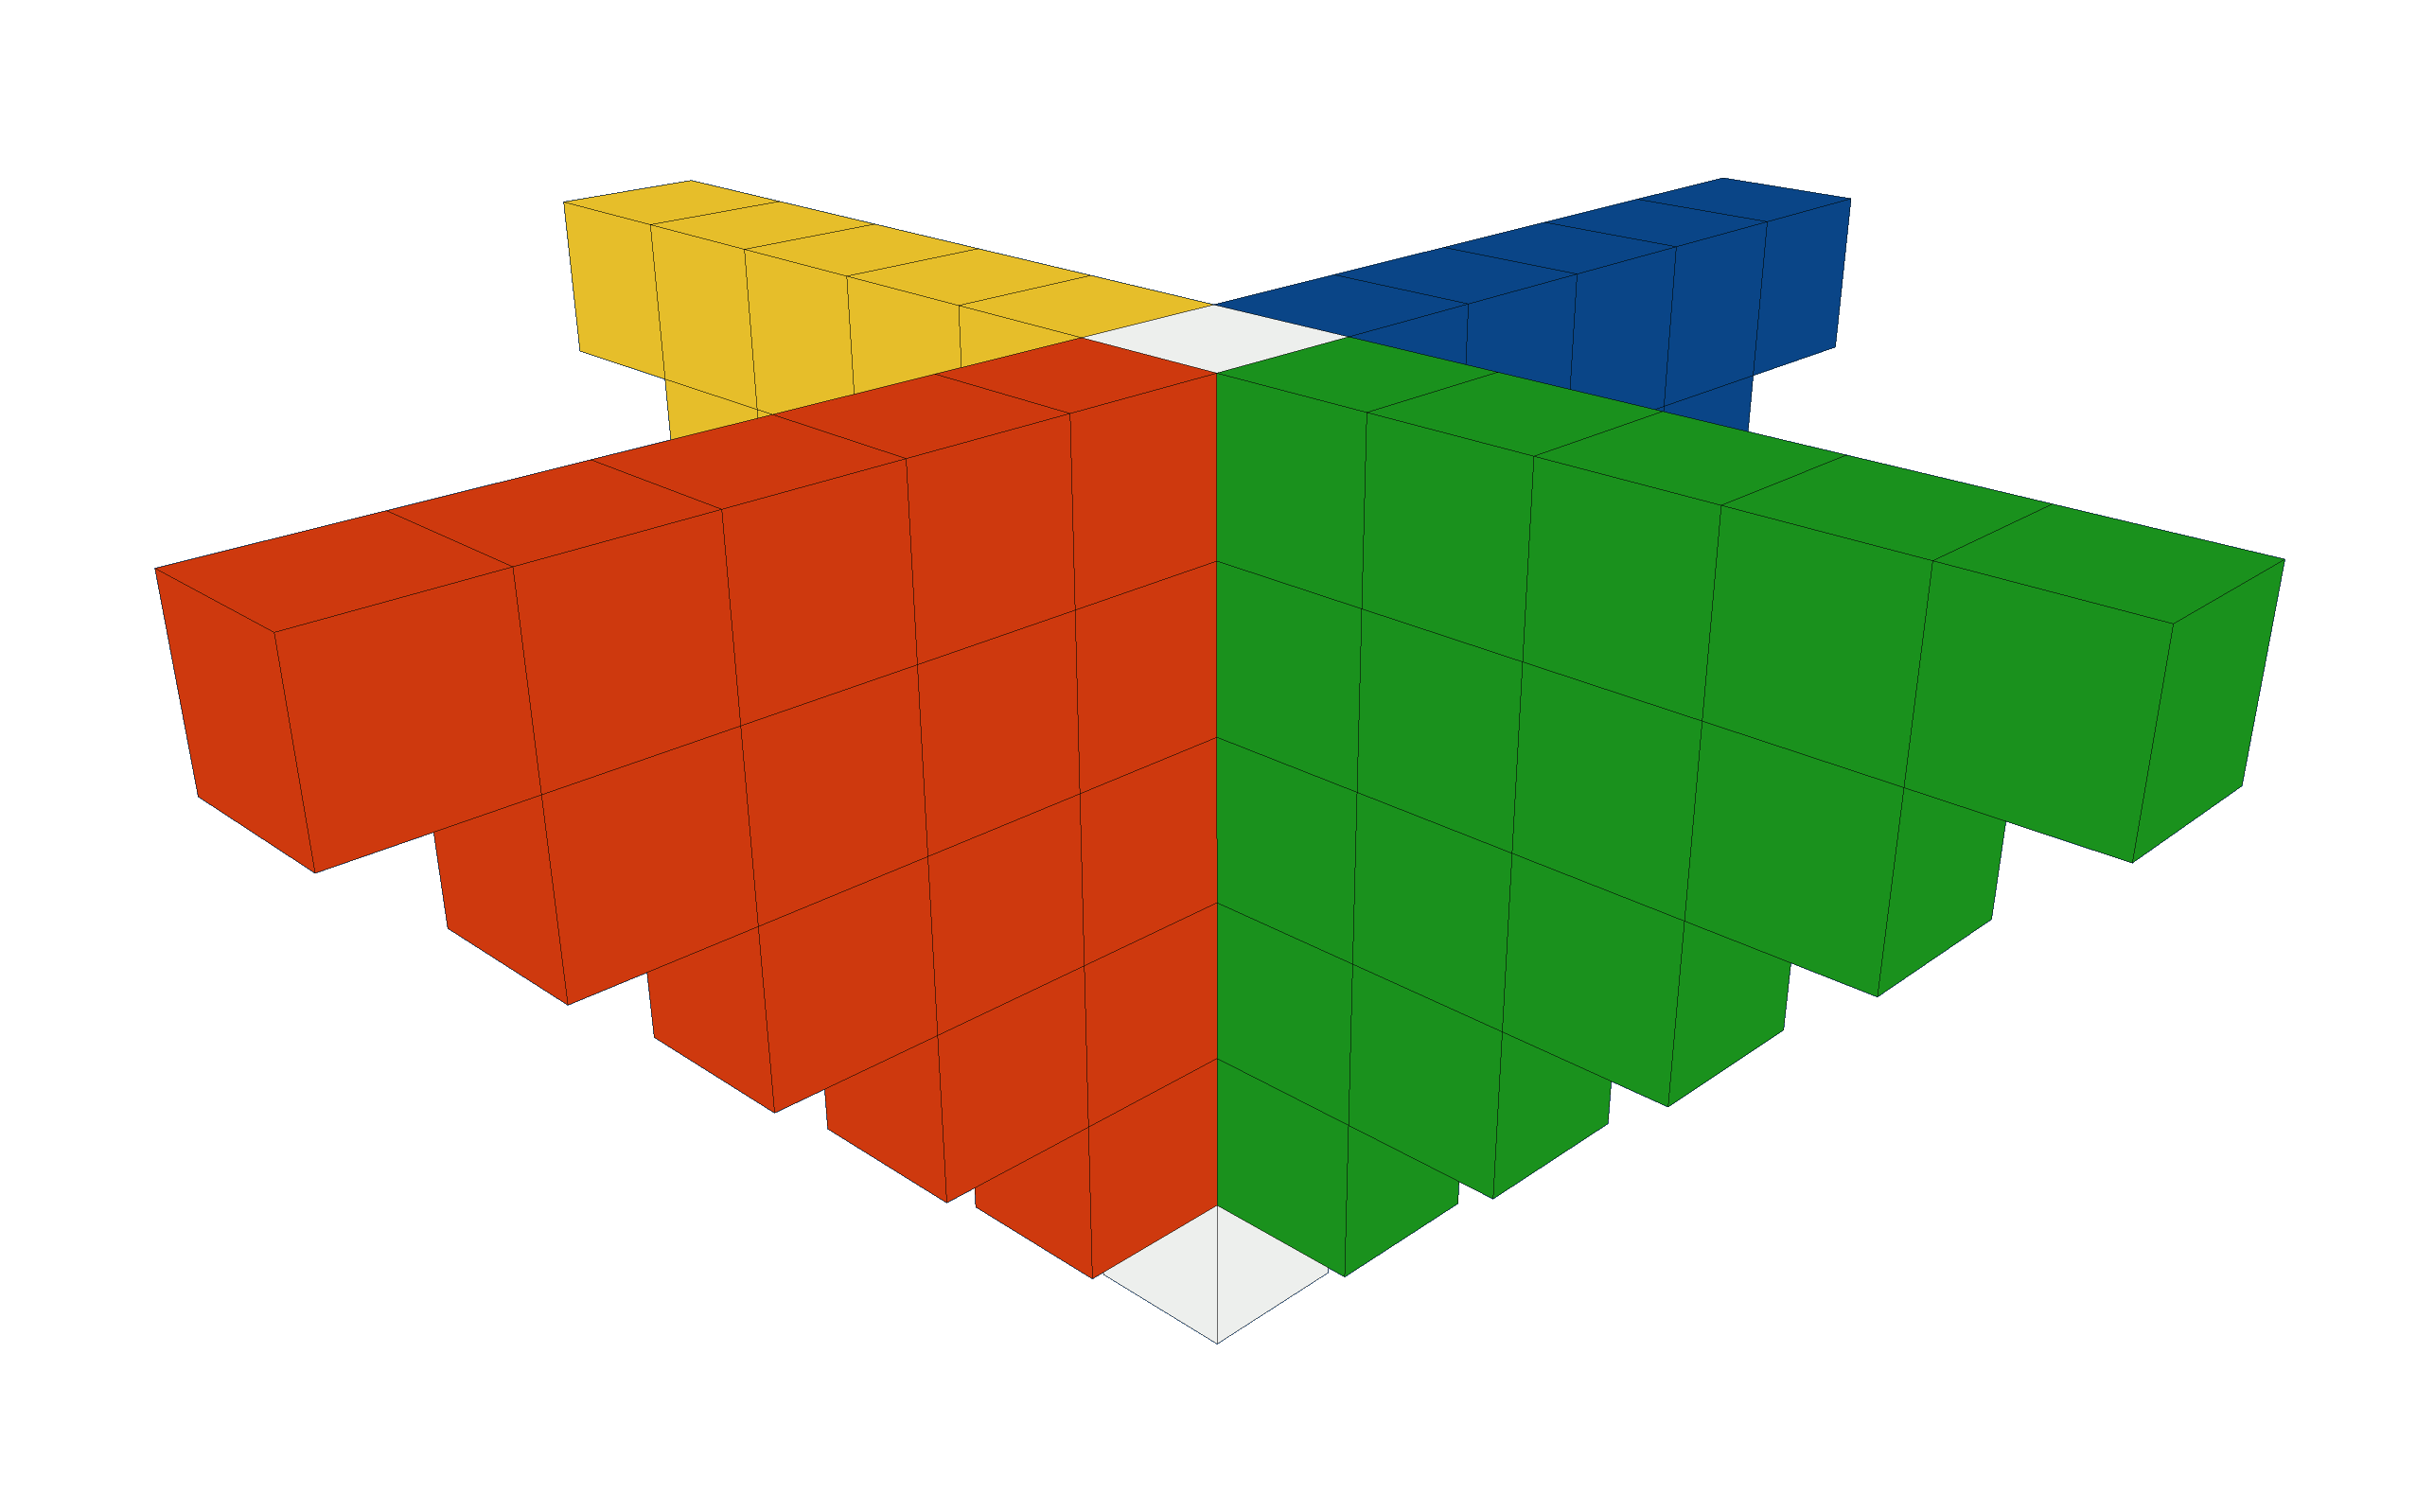
\includegraphics[height=0.093\textwidth]{../figures/angle1.png}\hspace{-5pt}
%    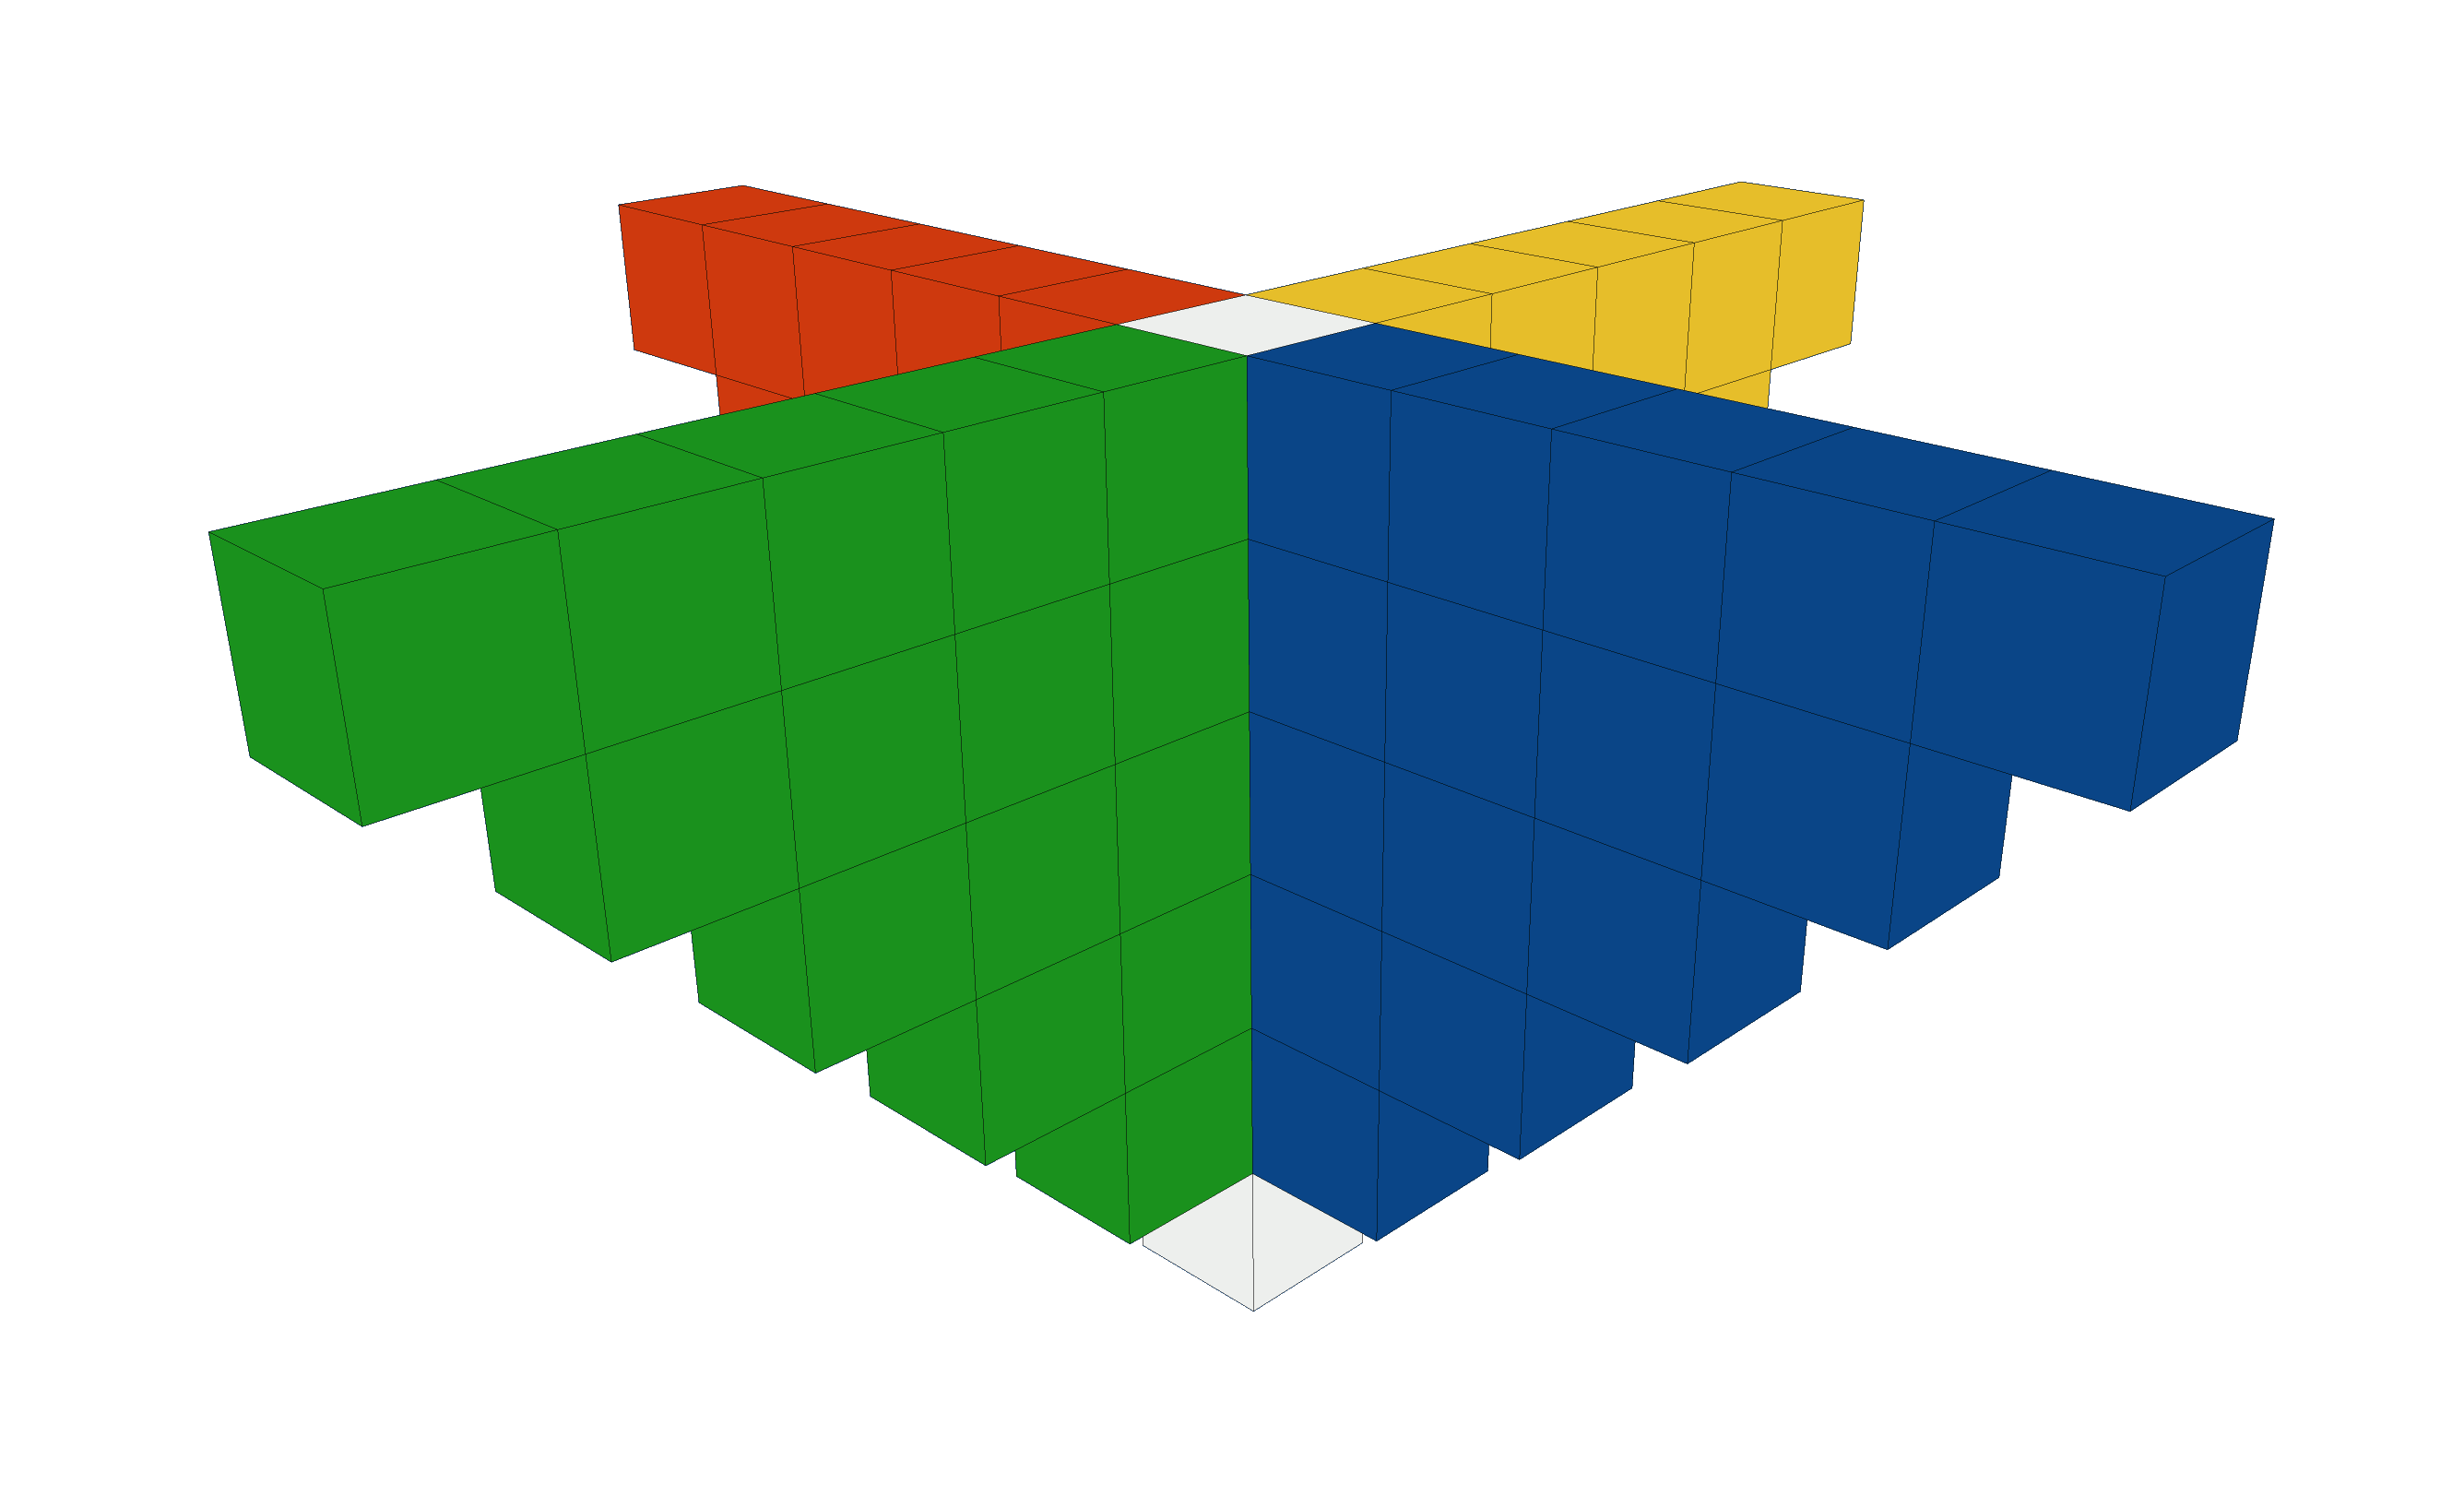
\includegraphics[height=0.093\textwidth]{../figures/angle2.png}\hspace{-5pt}
%    
\includegraphics[height=0.093\textwidth]{../figures/angle5.png}\hspace{-5pt}
%    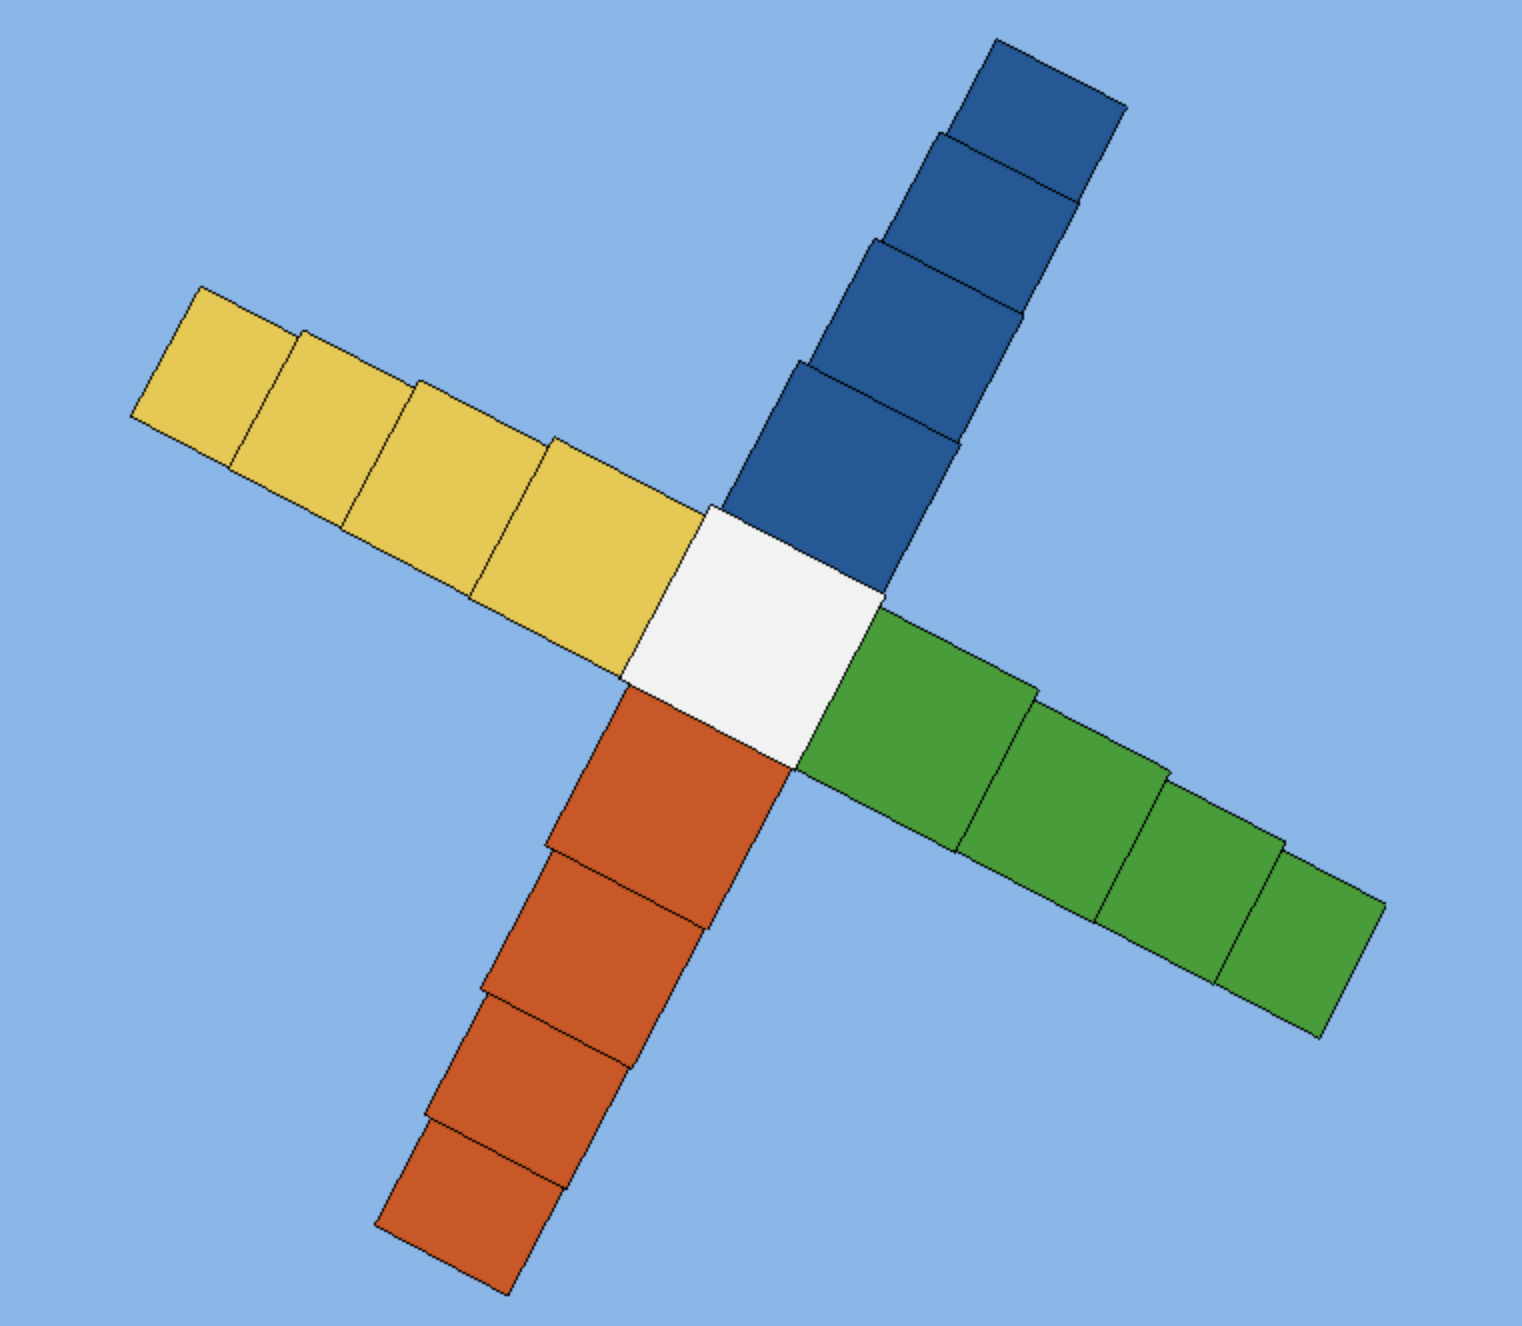
\includegraphics[height=0.093\textwidth]{../figures/angle3.png}\hspace{-3pt}
%    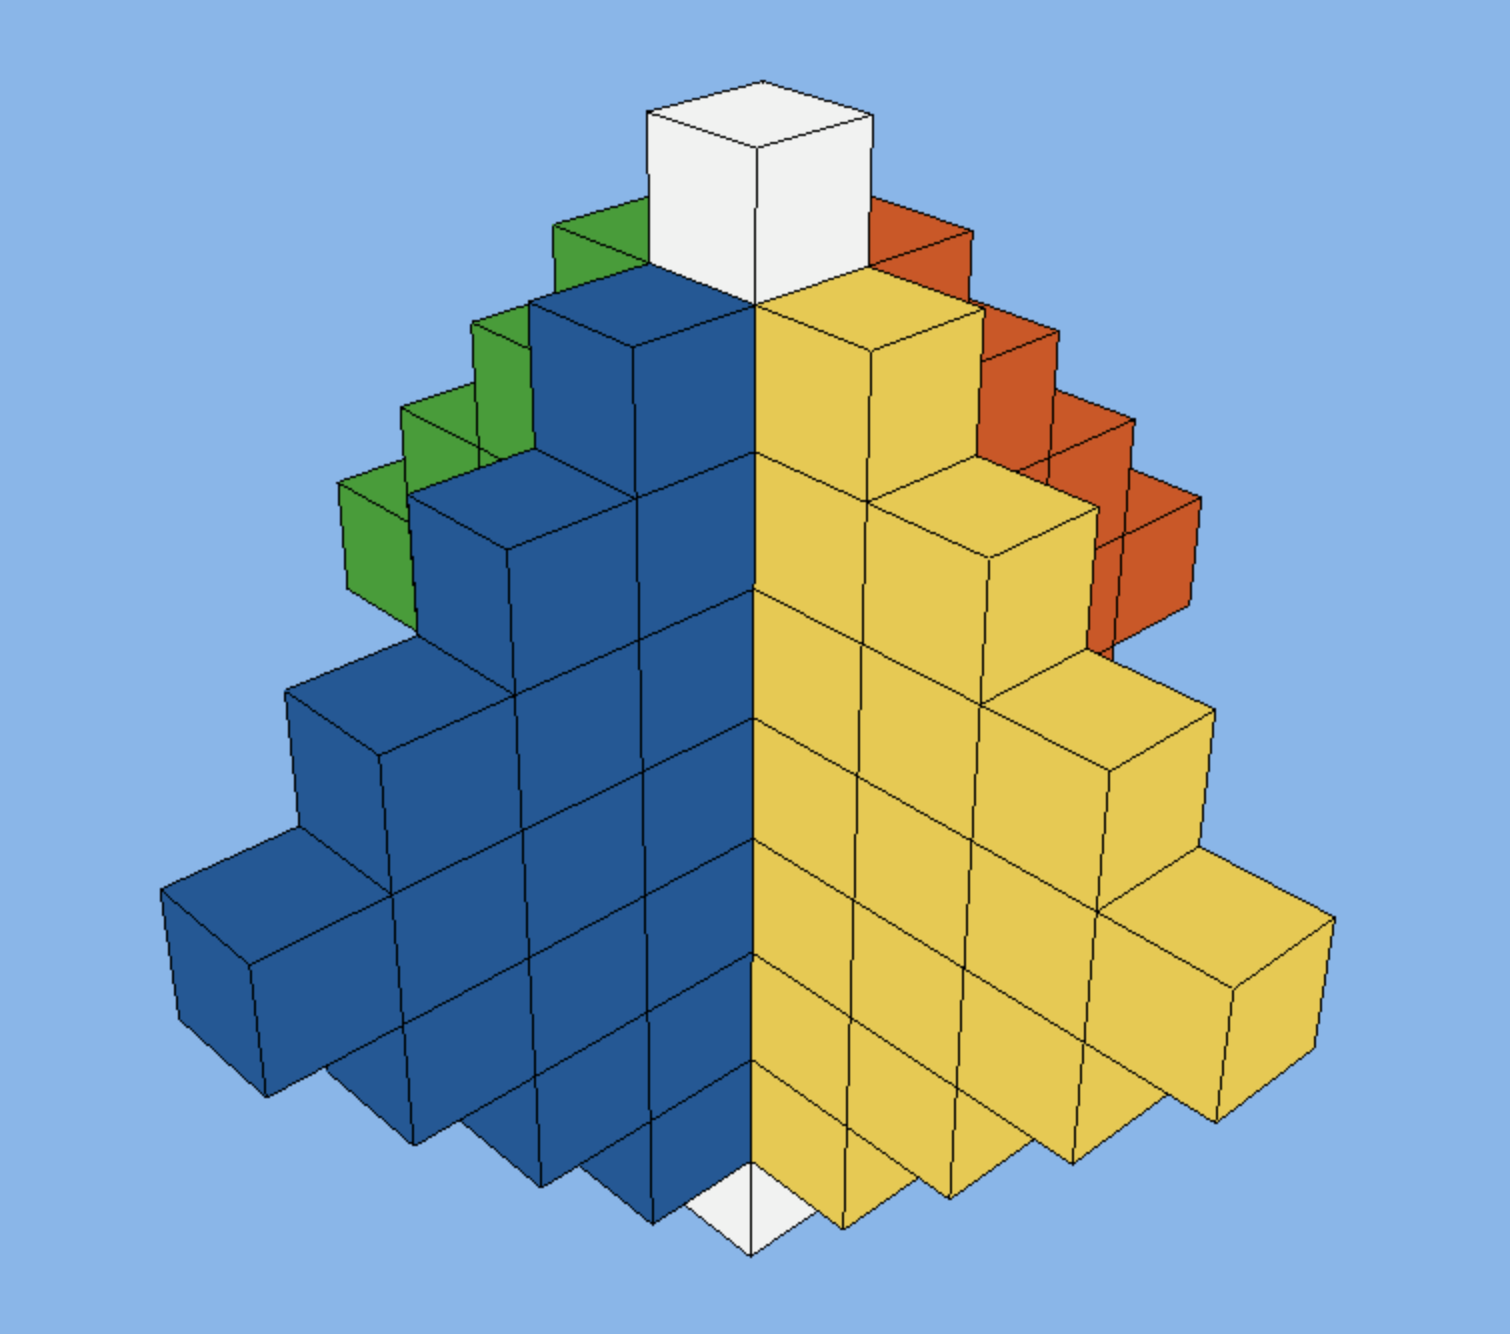
\includegraphics[height=0.093\textwidth]{../figures/angle4.png}
%  \end{figure}
%\end{frame}
%
%\begin{frame}[fragile]{An Simple Reachability Proof}
%  \begin{lemma}
%    For any nonempty language $\ell: \mathcal{L}(\mathcal{G})$ and invalid string $\err{\sigma}: \Sigma^n$, there exists an $(\tilde{\sigma}, m)$ such that $\tilde{\sigma} \in \ell\cap\Sigma^m$ and $0 < \Delta(\err{\sigma}, \ell) \leq \max(m, n) < \infty$, where $\Delta$ denotes the Levenshtein edit distance.\\
%  \end{lemma}
%
%  \begin{proof}
%    Since $\ell$ is nonempty, it must have at least one inhabitant $\sigma \in \ell$. Let $\tilde{\sigma}$ be the smallest such member. Since $\tilde{\sigma}$ is a valid sentence in $\ell$, by definition it must be that $|\tilde{\sigma}|<\infty$. Let $m:=|\tilde{\sigma}|$. Since we know $\err{\sigma} \notin \ell$, it follows that $0 < \Delta(\err{\sigma}, \ell)$. Let us consider two cases, either $\tilde{\sigma} = \varepsilon$, or $0 < |\tilde{\sigma}|$:
%
%    \begin{itemize}
%      \item If $\tilde{\sigma} = \varepsilon$, then $\Delta(\err{\sigma}, \tilde{\sigma}) = n$ by full erasure of $\err{\sigma}$, or
%      \item If $0 < m$, then $\Delta(\err{\sigma}, \tilde{\sigma}) \leq \max(m, n)$ by overwriting.
%    \end{itemize}
%
%    In either case, it follows $\Delta(\err{\sigma}, \ell) \leq \max(m, n)$ and $\ell$ is always reachable via a finite nonempty set of Levenshtein edits, i.e., $0 < \Delta(\err{\sigma}, \ell) < \infty$.
%  \end{proof}
%\end{frame}
%
%\begin{frame}[fragile]{Probabilistic repair generation}
%  \resizebox{\textwidth}{!}{
%    \begin{minipage}{1.4\textwidth}
%      \begin{algorithm}[H]
  \caption{Probabilistic reachability}
  \label{alg:adaptive}
  \begin{algorithmic}[1]
    \Require $\mathcal{G}$ grammar, $\err{\sigma}$ broken string, $p$ process ID, $c$ total CPU cores, $t_{\text{total}}$ timeout.
    \State $\mathcal{Q} \gets \varnothing, \mathcal{R} \gets \varnothing, \epsilon \gets 1, i \gets 0, Y \sim \mathbb{Z}_2^m, t_0 \gets t_{\text{now}}$ \Comment{Initialize replay buffer $\mathcal{Q}$ and reservoir $\mathcal{R}$.}
    \Repeat
      \If {$\mathcal{Q} = \varnothing$ or \textbf{Rand}(0, 1) $< \epsilon$}
        \State $\hat\sigma \gets \varphi^{-1}\left(\langle\kappa, \rho\rangle^{-1}(U^{ci+p}Y), \err{\sigma}\right), i \gets i + 1$ \Comment{Sample WoR using the leapfrog method.}
      \Else
        \State $\hat\sigma \sim \mathcal{Q} + \textbf{Noise}(\mathcal{Q})$ \Comment{Sample replay buffer with additive noise.}
      \EndIf
      \State $\mathcal{R} \gets \mathcal{R} \cup \{\hat\sigma\}$ \Comment{Insert repair candidate $\hat\sigma$ into reservoir $\mathcal{R}$.}
      \If{$\mathcal{R}$ is full}
        \State $\hat\sigma \gets \argmin_{\hat\sigma \in \mathcal{R}} PP(\hat\sigma)$ \Comment{Select lowest perplexity repair candidate.}
        \If{$\hat\sigma \in \mathcal{L}(\mathcal{G})$}
          \State $\mathcal{Q} \gets \mathcal{Q} \cup \{\hat\sigma\}$ \Comment{Insert successful repair into replay buffer.}
        \EndIf
        \State $\mathcal{R} \gets \mathcal{R} \setminus \{\hat\sigma\}$ \Comment{Remove checked sample from the reservoir.}
      \EndIf
      \State $\epsilon \leftarrow \textbf{Schedule}\big((t_{\text{now}} - t_0) / t_{\text{total}}\big)$ \Comment{Update exploration/exploitation rate.}
    \Until{$t_{\text{total}}$ elapses.}
    \State \Return $\tilde\sigma \in \mathcal{Q}$ ranked by $PP(\tilde\sigma)$.
  \end{algorithmic}
\end{algorithm}
%    \end{minipage}
%  }
%\end{frame}
%
%\begin{frame}[fragile]{Multicore Scaling Results (aarch64)}
%  \begin{tikzpicture}
%    \begin{axis}[
%      ybar,
%      enlargelimits=0.15,
%      legend style={at={(0.03,0.97)},anchor=north west},
%      title={\textbf{Relative Total Distinct Solutions Found vs. Single Core}},
%      x=1cm,
%      ylabel={Relative improvement},
%      xlabel={Number of assigned cores},
%      symbolic x coords={2,3,4,5,6,7,8,9,10},
%      xtick=data,
%      bar width=3pt,
%    ]
%      \addplot coordinates {
%        (2,0.1343) (3,0.1955) (4,0.2249) (5,0.2475)
%        (6,0.2760) (7,0.2994) (8,0.3073) (9,0.3151) (10,0.3229)
%      };
%      \addplot coordinates {
%        (2,0.2655) (3,0.4353) (4,0.5614) (5,0.6644)
%        (6,0.7462) (7,0.7783) (8,0.8347) (9,0.8005) (10,0.7798)
%      };
%      \addplot coordinates {
%        (2,0.3972) (3,0.6928) (4,0.9327) (5,1.1834)
%        (6,1.3138) (7,1.3988) (8,1.6039) (9,1.5500) (10,1.5691)
%      };
%      \addplot coordinates {
%        (2,0.4863) (3,0.8326) (4,1.1368) (5,1.3879)
%        (6,1.5873) (7,1.7494) (8,1.8802) (9,1.9059) (10,1.9625)
%      };
%      \addplot coordinates {
%        (2,0.4315) (3,0.7583) (4,1.0122) (5,1.2593)
%        (6,1.4586) (7,1.6349) (8,1.7813) (9,1.8324) (10,1.8695)
%      };
%      \legend{Holes=2,Holes=3,Holes=4,Holes=5,Holes=6}
%    \end{axis}
%  \end{tikzpicture}
%\end{frame}
\end{document}